%{{{-----------------------------------Basics----------------------------------%

%document class definition
\documentclass[
    11pt,
    a4paper,
    oneside,
    headinlcude, footinclude,
    twoside,
]{report}


%essential packages
\renewcommand*\rmdefault{ppl}
\usepackage[top=2.5cm,bottom=2.5cm,left=3cm,right=3cm]{geometry}
\usepackage[english]{babel}
\usepackage[T1]{fontenc}
\usepackage[utf8]{inputenc}
\usepackage{xcolor}
\usepackage{amssymb}


%additional packages
\usepackage{amssymb}
\usepackage{amsmath}
\usepackage[framemethod=Tikz]{mdframed} % for the "important" boxes
\usepackage{tikz} % to draw figures
\usepackage{enumerate} % to customize the type of enumerate you want
\usepackage{pgf,tikz,pgfplots} % for the transfer from geogebra to tikz
\usepackage{mathrsfs}% for the transfer from geogebra to tikz
\usepackage{graphicx} % to include pictures
\usepackage{stackrel}
\usepackage{fancyhdr}
\usepackage{tabularx}
\usepackage{makecell} % to make thick hlines in the front page
\usepackage[makeroom]{cancel}
%}}}

%{{{-----------------------------------Macros----------------------------------%

\newcommand{\myImplies}[0]{\rightarrow}

\newcommand{\powerset}[1]{\mathcal{P}(#1)}

\newcommand{\tvect}[3]{%
   \ensuremath{\Bigl(\begin{smallmatrix}#1\\#2\\#3\end{smallmatrix}\Bigr)}}

\newcommand{\myVector}[3]{\begin{pmatrix}#1\\#2\\#3\end{pmatrix}}

\newcommand{\tq}[0]{\textrm{t.q.}}

\newcommand{\markDate}[1]{\begin{flushright}#1\end{flushright}}

\newcommand{\cqfd}[0]{\begin{flushright}$\Box$\end{flushright}}

\renewcommand{\vec}[1]{\overrightarrow{#1}}

\def\getangle(#1)(#2)#3{
    \begingroup
        \pgftransformreset
        \pgfmathanglebetweenpoints{\pgfpointanchor{#1}{center}}{\pgfpointanchor{#2}{center}}
        \expandafter\xdef\csname angle#3\endcsname{\pgfmathresult}
    \endgroup
}

\newcommand\Warning{
    \makebox[1.4em][c]{
    \makebox[-5.5pt][c]{\raisebox{.2em}{!}}
    \makebox[0pt][c]{\color{red}\huge$\bigtriangleup$}}
}

%colored frame box
\newcommand{\cfbox}[2]{
    \colorlet{currentcolor}{.}
    {\color{#1}
    \fbox{\color{currentcolor}#2}}
}

\newcommand{\spring}[5]{
    \def\xo{#1};
    \def\yo{#2};
    \def\rayon{#3};
    \def\defasage{#4}; 
    \def\n{#5};
    \foreach \x in {1, ..., \n} 
    \draw ({\xo + \x*2*(\rayon -.5*\defasage)}, \yo) arc(0:180:\rayon); 

    \draw ({\xo + (\n+1)*2*(\rayon -.5*\defasage)}, \yo) arc(0:180:\rayon); 

    \foreach \x in {1, ..., \n} 
    \draw ({\xo +2*\rayon*\x -\defasage*\x -\defasage}, \yo) arc(180:360:.5*\defasage));
}

\makeatletter
\newcommand*{\inlineequation}[2][]{%
  \begingroup
    % Put \refstepcounter at the beginning, because
    % package `hyperref' sets the anchor here.
    \refstepcounter{equation}%
    \ifx\\#1\\%
    \else
      \label{#1}%
    \fi
    % prevent line breaks inside equation
    \relpenalty=10000 %
    \binoppenalty=10000 %
    \ensuremath{%
      % \displaystyle % larger fractions, ...
      #2%
    }%
    ~\@eqnnum
  \endgroup
}
\makeatother

%}}}

%{{{----------------------------------Settings---------------------------------%

\title{Physics}

\author{Arnò Fauconnet}

\setlength{\parindent}{0pt} %disable initial indent on first paragraph of sections in the whole doc

% the style of the boxes
\newmdenv[
        roundcorner=10pt,
        middlelinecolor=red,
        backgroundcolor=gray!15,
        linewidth=2pt,
        frametitlerule=true]{highlightBox}

% increases the space between paragraphs
\setlength{\parskip}{.3em}

\usetikzlibrary{calc}
\usetikzlibrary{arrows}%for the transfer from geogebra to tikz
\pgfplotsset{compat=1.15}


% Geogebras wierd colors xD
\definecolor{ffffff}{rgb}{1.,1.,1.}
\definecolor{qqqqff}{rgb}{0.,0.,1.}
\definecolor{qqffqq}{rgb}{0.,1.,0.}
\definecolor{ffqqtt}{rgb}{1.,0.,0.2}
\definecolor{ududff}{rgb}{0.30196078431372547,0.30196078431372547,1.} 
\definecolor{ffqqqq}{rgb}{1.,0.,0.} 
\definecolor{xdxdff}{rgb}{0.49019607843137253,0.49019607843137253,1.}
\definecolor{zzttqq}{rgb}{0.6,0.2,0.}
\definecolor{uuuuuu}{rgb}{0.26666666666666666,0.26666666666666666,0.26666666666666666}
\definecolor{wwccff}{rgb}{0.4,0.8,1.}
\definecolor{qqttcc}{rgb}{0.,0.2,0.8}
\definecolor{ffwwzz}{rgb}{1.,0.4,0.6}
\definecolor{ttqqqq}{rgb}{0.2,0.,0.}
\definecolor{qqccqq}{rgb}{0.,0.8,0.}
\definecolor{ffwwqq}{rgb}{1.,0.4,0.}
\definecolor{xfqqff}{rgb}{0.4980392156862745,0.,1.}
\definecolor{wwqqcc}{rgb}{0.4,0.,0.8}
\definecolor{qqzzqq}{rgb}{0.,0.6,0.}

\tikzstyle{every node}=[font=\large]

\graphicspath{ {./figures/} }


% header and footer settings
\pagestyle{fancy}
\fancyhf{}
\fancyhead[LE,LO]{Arnaud Fauconnet}
\fancyhead[CE,CO]{\textsc{Physique}}
\fancyhead[RE,RO]{MAN - Printemps 2019}
\fancyfoot[CE,CO]{\leftmark}
\fancyfoot[LE,RO]{\thepage}

\renewcommand{\headrulewidth}{2pt}
\renewcommand{\footrulewidth}{1pt}
%}}}

%%%%%%%%%%%%%%%%%%%%%%%%%%%%%%%%%%%%%%%%%%%%%%%%%%%%%%%%%%%%%%%%%%%%%%%%%%%%%%
%----------------------------------------------------------------------------%
%-------------------------------Text starts here-----------------------------%
%----------------------------------------------------------------------------%
%%%%%%%%%%%%%%%%%%%%%%%%%%%%%%%%%%%%%%%%%%%%%%%%%%%%%%%%%%%%%%%%%%%%%%%%%%%%%%


\begin{document}

\begin{titlepage}
   \begin{center}
       \vspace*{\fill}

       {\Huge EPFL}\\ 
%----------------------------------------------------------------------------%
       \vfill
       {\huge MAN}\\ [1em]
       {\Large Mise à niveau}\\
%----------------------------------------------------------------------------%
        \vfill
        \begin{tabularx}{\textwidth}{X}
            \Xhline{3\arrayrulewidth}\\
        \end{tabularx}\\ [2em]
        {\Huge Physique} \\ [1em]
        \textsc{\huge Prepa-033} \\ [2em]
        \begin{tabularx}{\textwidth}{X}
            \Xhline{3\arrayrulewidth}\\
        \end{tabularx}\\ [2em]
%----------------------------------------------------------------------------%
        \vspace{.7cm}
        {\large
        \begin{tabularx}{.9\textwidth}{Xr}
            \textit{Student:} & \textit{Professor:}\\
            Arnaud \textsc{Fauconnet} & Sylvain \textsc{Bréchet}
        \end{tabularx}}
%----------------------------------------------------------------------------%
        \vfill
        {\Large Printemps - 2019}

%----------------------------------------------------------------------------%
        \vfill
        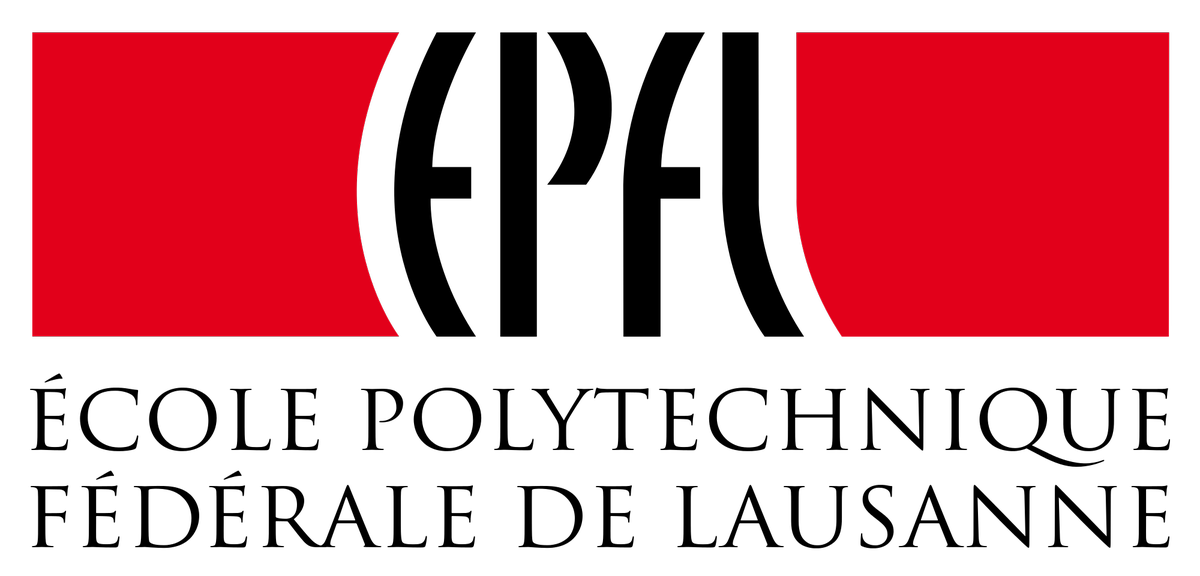
\includegraphics[width=7cm]{epfl-logo}

       \vfill
   \end{center} 
\end{titlepage}

%\chapter{Introduction (slides)}

%\chapter{Mouvement dans le plan}

%\section{Matière et espace}
%\label{sec:matiere_et_espace}

%\markDate{27/02/2019}

%La matière est faite d'atomes et de molécules. En mécanique classique, on peut
%considérer les molécules comme des petites billes en interaction.

%\begin{itemize}
    %\item 5 états:
        %\begin{enumerate}
            %\item Solide;
            %\item Liquide;
            %\item Gaz;
            %\item Plasma;
            %\item Condensat de Bose-Einstein;
        %\end{enumerate}
    %\item À l'échelle microscopique, on peut distinguer les atomes et les
        %molécules.
    %\item À l'échelle macroscopique, les atomes et les molécule forment un
        %continuum de matière.
    %\item Un object est un continuum
%\end{itemize}

%\subsection{Grandeurs extensives et intensives}
%\label{sub:grandeurs_extensives_et_intensives}

%\begin{itemize}
    %\item \textbf{Grandeurs extensives}: grandeur physique qui, pour un
        %ensemble d'objets, sont égalés à leur somme pour chaque objet.

        %\textbf{Exemple} quantité de matière, quantité de mouvement, force,
        %volume.

    %\item \textbf{Grandeur intensives}: grandeurs physique qui sont
        %indépendantes du nombre d'objets.

        %\textbf{Exemple} vitesse, accélération, temperature.
%\end{itemize}

%\subsection{Masse}
%\label{sub:masse}

%Masse ($M$ ou $m$): grandeur physique qui caractérise la quantité de matière
%d'un objet.
%\begin{itemize}
    %\item Grandeur extensive
    %\item Grandeur scalaire
    %\item Grandeur conservée (Lavoisier)
    %\item Masse constante $\implies$ système fermé (lingot d'or)
    %\item Masse variable $\implies$ système ouvert (fusée)
    %\item Unité physique (SI): kilogramme [ kg ]
%\end{itemize}

%\subsection{Volume}
%\label{sub:volume}

%Volume ($V$): grandeur physique scalaire et extensive qui caractérise la portion
%d'espace occupée par un objet.

%\begin{itemize}
    %\item Unité physique (SI): mètre cube [ m$^{3}$ ]
%\end{itemize}


%\subsection{Masse volumique}
%\label{sub:masse_volumique}

%Masse volumique ($\rho$): grandeur physique scalaire définie comme le rapport
%de la masse $m$ et du volume $V$.

%\begin{equation}
    %\rho = \frac{m}{V}
%\end{equation}

%\begin{itemize}
    %\item Unité physique (SI): [ $\frac{ \textrm{kg} }{ \textrm{m}^{3} }$ ]

    %\item Grandeur qui caractérise une matière
        %$\rho_{ \textrm{eau} } =  1 \ \frac{\textrm{kg} }{ \textrm{l}} =
        %10 ^{3} \ \frac{\textrm{kg}}{\textrm{m} ^{3}}; \rho_{ \textrm{glace} } =
        %0.9 \ \frac{\textrm{kg} }{ \textrm{l}} =
        %0.9 \cdot 10 ^{3} \ \frac{\textrm{kg}}{\textrm{m} ^{3}}$

    %\item \textbf{Homogène}: un objet est homogène si sa masse volumique est la
        %même partout (par ex. une planche de bois)

    %\item \textbf{Inhomogène}: un objet est inhomogène si sa masse volumique
        %varie d'un endroit à l'autre (par ex. un marteau avec manche en bois
        %et tête en fer)
%\end{itemize}

%\subsection{Densité}
%\label{sub:densite}

%Densité ($d$): nombre sans dimension physique définie comme le rapport entre
%la masse volumique de l'objet et la masse volumique de l'eau.

%\begin{equation}
    %d = \frac{\rho}{\rho_{ \textrm{eau} }}
%\end{equation}

%\subsection{Surface}
%\label{sub:surface}

%Surface ($s, \sigma$): grandeur physique scalaire et extensible qui
%caractérise une portion de l'espace en à deux dimensions.

%\begin{itemize}
    %\item Unité physique (SI): mètre carré [ m$^{2}$ ]
%\end{itemize}

%\subsection{Longueur}
%\label{sub:longueur}

%Longueur ($l, x, r, s, d, L$): grandeur physique scalaire et extensible de
%l'espace à une dimension.

%\begin{itemize}
    %\item Unité physique (SI): mètre [ m ]
%\end{itemize}


%\section{Référentiel}
%\label{sec:referentiel}

%\subsection{Point matériel}
%\label{sub:point_materiel}

%Représentation  d'un object par rapport à un point auquel on associe toute la
%matière (masse) de l'objet.

%\begin{itemize}
    %\item \textbf{Modèle}: idéalisation de la réalité
    %\item \textbf{Limites}: pas de mouvement de rotation propre
    %\item \textbf{Erreurs}: (i) quantitatif, (ii) qualitatif
%\end{itemize}

%\subsection{Référentiel}
%\label{sub:referentiel}

%\begin{itemize}
    %\item Object physique (indéformable) de référence par rapport auquel on
        %décrit le mouvement.

        %\textbf{Exemple}: terre, bateau, système solaire
    %\item Un ensemble de $N$ points matériels ($N \geq 4$) non-complanaires et fixes
        %les uns par rapport aux autres.
%\end{itemize}


%\markDate{28/02/2019}

%\subsection{Repère}
%\label{sub:repere}

%Un \textbf{repère} est une \textbf{entité géométrique}. Dans le plan, c'est à
%dire dans un espace à 2 dimensions, un repère est constitué de 2 vecteurs
%linéairement indépendants (i.e. non colinéaire) attachés à un point appelé
%l'\textbf{origine} $O$.

%\begin{itemize}
    %\item Repère quelconque:

        %\begin{center}
            %\begin{tikzpicture}[>= latex]
                %\draw [->] (0, 0) node[anchor= north east] {$0$} -- (1, 1)
                %node [anchor=east] {$\vec y$};

                %\draw [->] (0, 0) -- (2, 0) node [anchor=north] {$\vec x$};
            %\end{tikzpicture}
        %\end{center}

    %\item Un repère est orthonormé si et seulement si les vecteurs de base
        %$\vec{e_{x}}$ et $\vec{e_{y}}$ sont orthogonales ($\vec{e_{x}} \perp
        %\vec{e_{y}}$) et unitaires ($\| \vec{e_{x}} \| = \| \vec{e_{y}} \| = 1$)

    %\pagebreak

    %\item Repère horizontale-vertical ($0, \vec{e_{x}}, \vec{e_{y}}$)
        %\begin{center}
            %\begin{tikzpicture}[>= latex]
                %\draw [->] (0, 0) node[anchor= north east] {$0$} -- (0, 1)
                %node [anchor=east] {$\vec{e_{y}}$};
                %\draw [->] (0, 0) -- (1, 0) node [anchor=north] {$\vec{e_{x}}$};
            %\end{tikzpicture}
        %\end{center}

    %\item  Repère oblique ($0, \vec{e_{x}}, \vec{e_{y}}$)
        %\begin{center}
            %\begin{tikzpicture}[>= latex]
                %\draw [->] (0, 0) node[anchor= east] {$0$} -- (1, 1)
                %node [anchor=south] {$\vec{e_{y}}$};
                %\draw [->] (0, 0) -- (1, -1) node [anchor=north] {$\vec{e_{x}}$};
            %\end{tikzpicture}
        %\end{center}
%\end{itemize}

%\Warning référentiel (physique: \textbf{réel})  $\iff$ repère (géométrique:
%\textbf{virtuel}) \Warning

%\section{Vecteur position et déplacements}
%\label{sec:vecteur_position_et_deplacements}

%\subsection{Vecteur position}
%\label{sub:vecteur_position}

%\begin{itemize}
    %\item La position d'un objet (point materiel) dans le référentiel est
        %donné par le vecteur position $\vec r$:
        %\begin{center}
            %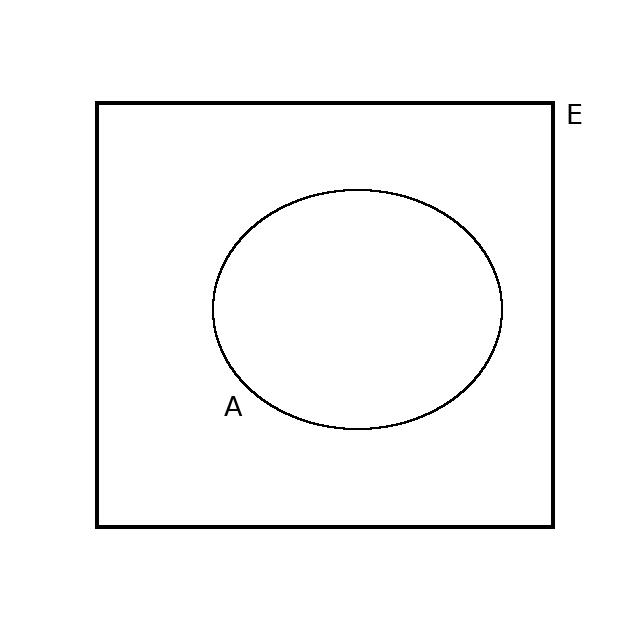
\includegraphics[width=5cm]{fig1}
        %\end{center}

    %\item Unité physique (SI): mètre [ m ]
%\end{itemize}

%\paragraph{Vecteur}
%\label{par:vecteur}

%Un vecteur possède 3 propriétés fondamentale:

%\begin{itemize}
    %\item Direction
    %\item Sens
    %\item Norme
%\end{itemize}

%On le note par un symbole surmonté d'une flèche (manuscrit) ou en gras
%(caractère d'imprimerie)

%Pour le vecteur position \textbf{r}, la \textbf{direction} est la droite
%passant pas $O$ et l'objet, le \textbf{sens} est donné par le regard vers
%l'objet depuis $O$ et la \textbf{norme} par la distance de $O$ à l'objet.

%\begin{itemize}
    %\item Le vecteur position $\vec r$ peut être décomposé dans le repère orthonormée
        %$(O, \vec{e_{x}}, \vec{e_{y}})$

        %\begin{center}
            %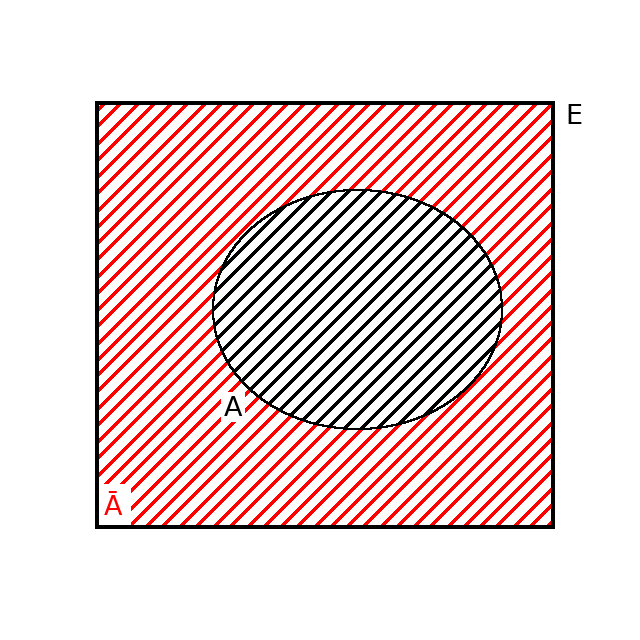
\includegraphics[width=5cm]{fig2.png}
        %\end{center}

    %\item Vecteur position $\vec r$:

        %\begin{equation}
            %\vec r = x \cdot \vec{e_{x}} + y \cdot \vec{e_{y}} = \myVector{x}{y}{}
            %= \myVector{\cos(\alpha)\cdot r}{\sin(\alpha)\cdot r}{}
         %\end{equation}

         %$$ \textrm{où}\ r = \| \vec r \| = \sqrt{x^{2} + y^{2}}$$
         
         %$x$ et $y$ sont les \textbf{composants} du vecteurs position $\vec r$
         %dans le repère orthonormée $(O, \vec{e_{x}}, \vec{e_{y}})$

    %\item Comme l'objet peut se déplacer au cours du temps, sa position peut
        %changer.
%\end{itemize}

%\subsection{Temps}
%\label{sub:temps}

%Temps ($t$ ou $T$): grandeurs scalaire qui décrit l'évolution d'un système
%physique.

%\begin{itemize}
    %\item Unité physique (SI): secondes [ s ]

    %\item Comme un objet se déplace au cours du temps, son vecteur position
        %est function du temps: $\vec r \equiv \vec r (t)$

    %\item Vecteur position à l'instant $t$:

        %\begin{equation}
            %\vec r (t) = x(t) \cdot \vec{e_{x}} + y(t) \cdot \vec{e_{y}} =
            %\myVector{x(t)}{y(t)}{} = \myVector{r(t) \cdot \cos(\alpha(t))}{r(t) \cdot \sin(\alpha(t))}{}
        %\end{equation}

    %\item \textbf{Exemples}: horaires de train (Où? Quand?), GPS
%\end{itemize}

%\subsection{Trajectoire}
%\label{sub:trajectoire}

%\begin{itemize}
    %\item Lieux géométrique des points de l'espace occupés par l'objet (point
        %matériel) au cours du temps.

    %\pagebreak

    %\item Ensemble des points qui sont atteints par l'objet (courbe ou droite)
        %représenté par $\Gamma$

        %\begin{center}
            %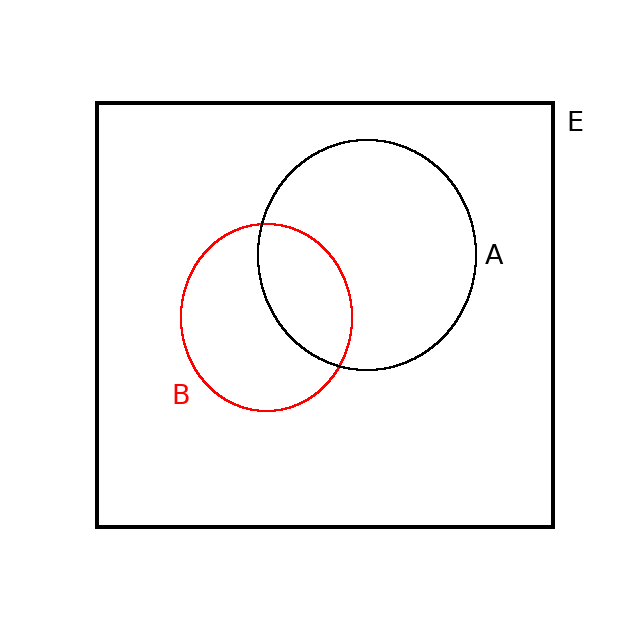
\includegraphics[width=8cm]{fig3}
        %\end{center}
%\end{itemize}


%$$\Gamma = \{ P | \exists t, \vec{OP} = \vec r (t)\}$$

%\paragraph{Exemples}
%\label{par:exemples}

%\begin{enumerate}
    %\item Droite (chute libre)
    %\item Cercle (electron dans un champ magnétique)
    %\item Parabole (projectile)
    %\item Ellipse (planète)
    %\item Hyperbole (astéroïde)
%\end{enumerate}

%La trajectoire répond à la question "où?" sans se préoccuper de la question
%"quand?".

%\pagebreak

%\subsection{Déplacement}
%\label{sub:deplacement}

%Le vecteur déplacement est la variation du vecteur position au cours du temps.
%On considère les position $P_{1}$ et $P_{2}$ d'un objet aux temps $t_{1}$ et $t_{2}$
%où $t_{1} < t_{2}$.

%\begin{center}
    %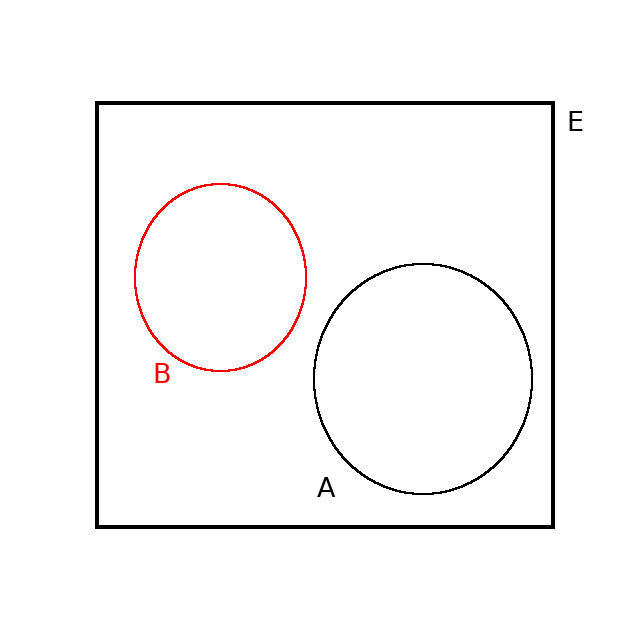
\includegraphics[width=8cm]{fig4}
%\end{center}

%$$\vec{r_{1}} + \Delta \vec r = \vec{r_{2}}$$

%\begin{itemize}
    %\item Déplacement le long de 
        %\begin{equation}
            %\Gamma: \Delta \vec r = \vec{r_{2}} - \vec{r_{1}} = \vec r (t_{1}) - \vec r (t_{1})
        %\end{equation}

    %\item \textbf{Exemple}: Le vecteur déplacement $\Delta \vec r$ entre
        %Genève (position $\vec{r_{1}}$) et Lausanne (position $\vec{r_{2}}$) le
        %long des voies le chemin de fer (trajectoire $\Gamma$)
%\end{itemize}

%\paragraph{Cas particuliers:}
%\label{par:cas_particuliers_}

%\begin{enumerate}
    %\item Objet immobile au point $A$

        %\begin{center}
            %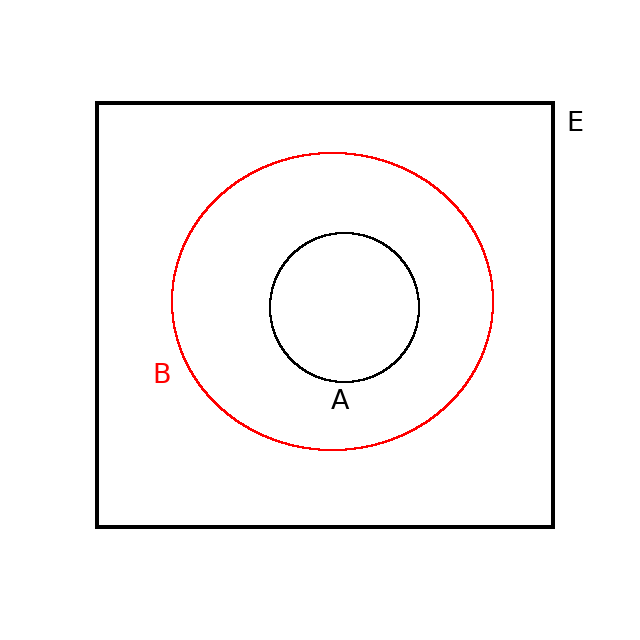
\includegraphics[width=5cm]{fig5}
        %\end{center}

        %Vecteur position indépendant du temps $t$: 

        %\begin{equation}
            %\label{eq:rt_cste}
            %\vec r (t) = \vec{OA} = \vec{r_{0}} = \vec{cste} \quad \forall t
        %\end{equation}

    %\item Objet qui avance régulièrement  sur une droite $\Gamma$ qui passe
        %par un point $A$ l'instant $t_{0}: \vec r (t_{0}) = \vec{OA} =
        %\vec{r_{0}}$

        %\begin{center}
            %\begin{tikzpicture}[line cap=round,line join=round,>=triangle 45,x=1.0cm,y=1.0cm]
                %\begin{axis}[
                %x=1.0cm,y=1.0cm,
                %axis lines=middle,
                %xmin=-0.7,
                %xmax=6.0,
                %ymin=-0.7,
                %ymax=6.0,
                %xtick={0.0,1.0,...,5.0},
                %ytick={0.0,1.0,...,5.0},]
                %\clip(-0.7,-0.7) rectangle (6.,6.);
                %\draw [->,line width=0.5pt] (0.,0.) -- (0.9912936274413515,4.066851325623913) node [anchor=south,color=ududff] {$A$};
                %\draw [->,line width=0.5pt] (0.,0.) -- (3.9237546376441306,1.8428441986199695) node [anchor=south,color=ududff] {$P$};
                %\draw [line width=0.5pt,color=qqqqff,domain=-0.7:6.] plot(\x,{(--14.13052703906677-2.2240071270039437*\x)/2.932461010202779}) node [anchor = east]{$\Gamma$};
                %\draw [->,line width=0.7pt,color=ffqqqq] (0.9912936274413515,4.066851325623913) -- (2.1358112820513946,3.1988379361948893) node [color=ffqqqq, midway,anchor=south] {$\vec{v_{0}}$};
                %\draw [->,line width=0.7pt,color=ffqqqq] (3.9237546376441306,1.8428441986199695) -- (5.068272292254173,0.9748308091909454) node [color=ffqqqq, midway,anchor=south] {$\vec{v_{0}}$};
                %\begin{scriptsize}
                %\draw [fill=ududff] (0.9912936274413515,4.066851325623913) circle (1.5pt);
                %\draw[color=black] (0.5025501257408889,2.2912327322901245) node [anchor=west] {$\vec{r_{0}}$};
                %\draw [fill=ududff] (3.9237546376441306,1.8428441986199695) circle (1.5pt);
                %\draw[color=black] (2.5696212659602815,0.7891311444951222) node {$\vec r(t)$};
                %\draw[color=qqqqff] (-0.11174216538721699,4.555594827324382) ;
                %\end{scriptsize}
                %\end{axis}
                %\end{tikzpicture}
        %\end{center}

        %\begin{itemize}
            %\item Le vecteur déplacement $\Delta \vec r = \vec r (t) -
                %\vec{r_{0}}$ est proportionnelle à sa durée $\Delta t = t -
                %t_{0}$

            %\item Il existe un vecteur directeur $\vec{v_{0}}$ de la droite
                %tel que $\Delta \vec r = \vec{v_{0}} \cdot \Delta t$, ou
                %encore 

                %\begin{equation}
                    %\vec r (t) = \vec{v_{0}} \cdot (t - t_{0}) + \vec{r_{0}} 
                    %\label{eq:2.7}
                %\end{equation}
        %\end{itemize}

        %\item L'objet est dit en mouvement rectiligne uniforme (MRU)

        %\item Dans le plan, on donne l'origine $O$ et un point $A$. Un objet
            %se déplace de $O$ à $A$ entre $t = 0$ et $t = t_{A}$

        %\item On cherche à déterminer l'équation horaire $\vec r (t)$ de
            %l'objet en considérant que celui-ci passe en $O$ à l'instant $t =
            %0$.

            %\begin{center}
                %\includegraphics[width=8cm]{fig7}
            %\end{center}

        %\item Conditions l'initiale et finale: $\vec r (0) = \vec 0$ et $\vec
            %r (t_{A}) = \vec{OA}$

        %\item Ainsi: 
            %\begin{equation}
                %\vec r (t_{A}) = \vec{v_{0}} \cdot t_{A} = \vec{OA} \implies
                %\vec{v_{0}} = \frac{\vec{OA}}{t_{A}}
            %\end{equation}

        %\item Finalement, \begin{equation}\vec r (t) = \vec{v_{0}} \cdot t = \frac{t}{t_{A}}
                %\cdot \vec{OA}\end{equation}

        %\item \textbf{Rencontre}: Lorsque deux objets se trouvent à la même
            %position au même temps $t_{r}$, il y a rencontre

            %\begin{equation}
                %\exists t_{r} \vec{r_{1}} (t_{1}) = \vec{r_{2}} (t_{r})
            %\end{equation}
%\end{enumerate}

%\section{Vecteur vitesse}
%\label{sec:vecteur_vitesse}

%\subsection{Vitesse moyenne}
%\label{sub:vitesse_moyenne}

%On considère un objet en position initiale $P_{1}$ au temps initiale $t_{1}$
%et en position finale $P_{2}$ au temps finale $t_{2}$

%\begin{center}
    %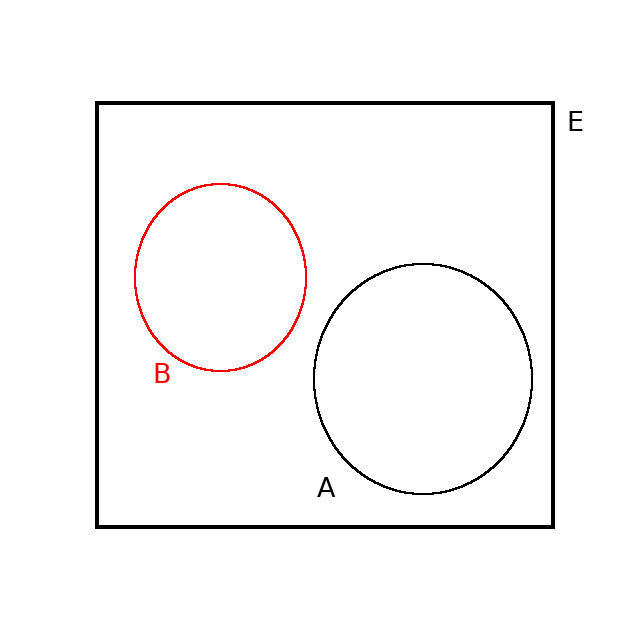
\includegraphics[width=8cm]{fig4}
%\end{center}

%\begin{itemize}
    %\item Position initiale: $\vec{r_{1}} = \vec r (t_{1})$
    %\item Position finale: $\vec{r_{2}} = \vec r (t_{2})$
    %\item Déplacement: $\Delta \vec r = \vec{r_{2}} - \vec{r_{1}}$
    %\item Intervalle de temps: $\Delta t = t_{2} - t_{1}$
%\end{itemize}


%\begin{itemize}
    %\item La \textbf{vitesse moyenne} ($\vec{v_{moy}}$) de l'objet est définie
        %comme le rapport entre le déplacement $\Delta \vec r$ et l'intervalle
        %de temps $\Delta t$

        %\begin{equation}
            %\vec{v_{moy}} = \frac{\Delta \vec r}{\Delta t} 
        %\end{equation}

    %\item Unité physique (SI): mètre par secondes 
        %[ $\frac{\textrm{m}}{\textrm{s}}$ ]

    %\item La vitesse moyenne ne donne que la position finale $\vec{r_{2}}$ par
        %rapport à la position initiale $\vec{r_{1}}$ et non les positions
        %intermédiaires 

        %\begin{equation}
            %\vec{r_{2}} = \vec{r_{1}} + \vec{v_{moy}} \cdot \Delta t
        %\end{equation}
        
    %\item C'est  la vitesse constante qu'il faudrait maintenir pour faire le
        %déplacement $\Delta \vec r$ durant l'intervalle du temps $\Delta t$.
%\end{itemize}

%\begin{center}
    %\begin{minipage}{.5\linewidth}
        %\resizebox{\textwidth}{!}{
            %\begin{tikzpicture}[line cap=round,line join=round, >= latex,x=1.0cm,y=1.0cm]
            %\tikzstyle{every node}=[font=\scriptsize]
            %\begin{axis}[
            %x=1.0cm,y=1.0cm,
            %axis lines=middle,
            %xmin=-0.5,
            %xmax=4.0,
            %ymin=-0.5,
            %ymax=4.5,
            %xtick={-0.0,1.0,...,3.0},
            %ytick={-0.0,1.0,...,4.0},]
            %\clip(-0.5,-0.5) rectangle (4.,5.);
            %\draw [samples=50,rotate around={-228.3882158815608:(1.63721103787723,2.780353297122578)},xshift=1.63721103787723cm,yshift=2.780353297122578cm,line width=1pt,color=qqqqff,domain=-6.184162744813402:6.184162744813402)] plot (\x,{(\x)^2/2/1.5460406862033504});
            %\draw [->,line width=.5pt] (0.,0.) -- (1.4054298862371315,2.993507684986792);
            %\draw [->,line width=.5pt] (0.,0.) -- (1.475367905161338,2.9378595326316175);
            %\draw [->,line width=.5pt] (1.4054298862371315,2.993507684986792) -- (1.475367905161338,2.9378595326316175);
            %\draw [dash pattern=on 1pt off 1pt,color=qqccqq,domain=-0.5:4.] plot(\x,{(--0.28756957355620383-0.055648152355174396*\x)/0.06993801892420648});
            %\draw [->,line width=0.5pt,color=qqccqq] (1.4054298862371315,2.993507684986792) -- (2.3295147609991482,2.2582335566818714);
            %\draw[color=black] (0.598112073142613,1.8097492393092884) node {$\vec{r_{1}}$};
            %\draw[color=black] (1.006788281285858,1.427564527508181) node {$\vec{r_{2}}$};
            %\draw[color=black] (1.5949506619244465,3.1712822751007335) node {$\Delta \vec r$};
            %\draw[color=qqccqq] (1.9760136127607153,2.7140255663386945) node {$\vec v$};
            %\end{axis}
            %\end{tikzpicture}
        %}
    %\end{minipage}
    %\begin{minipage}{.49\linewidth}
        %\begin{itemize}
            %\item Dans la limite où l'intervalle de $\Delta t$ est très petit,
                %le déplacement 
                %\begin{equation}\Delta \vec r = \vec{r_{2}} - \vec{r_{1}}\end{equation}
                %donne la direction et le sens de mouvement est juste après le
                %temps $t_{1}$.
            %\item Le déplacement $\Delta \vec r$ devient vecteur directeur de
                %la tangente à la trajectoire en $\vec{r_{0}}$ 
        %\end{itemize}
    %\end{minipage}
%\end{center}

%\begin{itemize}
    %\item La \textbf{vitesse instantanée} ou \textbf{vitesse} de l'objet est
        %définie comme la vitesse moyenne dans la limite d'un intervalle du
        %temps infinitésimale.

        %\begin{equation}
            %\label{eq:2.13}
            %\vec v (t) = \lim_{\Delta t \to 0} \frac{\Delta \vec r}{\Delta t}
            %= \lim_{\Delta t \to 0} \frac{\vec r (t + \Delta t) - \vec r (t)}{\Delta t}
            %= \frac{d\vec r}{dt} = \dot{\vec r} (t)
        %\end{equation}
%\end{itemize}

%\paragraph{Propriétés de la vitesse}
%\label{par:proprietes_de_la_vitesse}

%\markDate{6/03/2019}


%\begin{itemize}
    %\item Taux de variation de la position par rapport au temps (dérivée)
    %\item Vector (direction, sens, norme)
    %\item Tangente à la trajectoire dans le sens du mouvement
%\end{itemize}



%\paragraph{Cas particuliers}

%\begin{enumerate}
    %\item Objet immobile qui se trouve au point A

        %\begin{center}
            %\begin{minipage}{.5\linewidth}
                %\resizebox{\textwidth}{!}{
                    %\begin{tikzpicture}[line cap=round,line join=round,>=triangle 45,x=1.0cm,y=1.0cm]
                    %\begin{axis}[
                    %x=1.0cm,y=1.0cm,
                    %axis lines=middle,
                    %xmin=-0.5,
                    %xmax=5.9,
                    %ymin=-0.19595529090418443,
                    %ymax=5.656623567248618,
                    %xtick={-0.0,1.0,...,5.0},
                    %ytick={-0.0,1.0,...,5.0},]
                    %\clip(-0.5,-0.19595529090418443) rectangle (5.9,5.656623567248618);
                    %\draw [->,] (0.,0.) -- (5.213746581801192,4.798140383149461) node[midway,
                    %anchor= south east] {$\vec r_{0}$};
                    %\begin{scriptsize}
                        %\draw [fill=ududff] (5.213746581801192,4.798140383149461) circle (1.5pt) node[anchor=south] {$A$};
                    %\draw[color=ududff] (5.347619047619048,4.896413146171829);
                    %\draw[color=black] (2.3,2.601896761095316) ;
                    %\end{scriptsize}
                    %\end{axis}
                    %\end{tikzpicture}
                %}
            %\end{minipage}
            %\begin{minipage}{.4\linewidth}
                %Vecteur vitesse nulle (position constante):
                %\begin{equation}
                    %\vec v(t) = \vec 0, \quad \forall t
                %\end{equation}
                %$$ \text{ car } \vec r (t) = \vec{0A} = \vec{r_{0}} \quad (\ref{eq:rt_cste})$$
            %\end{minipage}
        %\end{center}

        %\paragraph{Vérification:}
        %\label{par:verification}

        %$$\vec v (t) = \lim_{\Delta t \to 0} \frac{\vec r ( t + \Delta t) - \vec r (t)}{\Delta t} 
        %= \lim_{\Delta t \to 0} \frac{\vec{r_{0}} - \vec{r_{0}}}{\Delta t} = \vec 0 $$

        %\cqfd
    %\item Objet qui avance  à vitesse constante 

        %\begin{center}
            %\begin{minipage}{.5\linewidth}
                %\resizebox{\textwidth}{!}{
                    %\begin{tikzpicture}[line cap=round,line join=round,>=triangle 45,x=1.0cm,y=1.0cm]
                        %\begin{axis}[
                        %x=1.0cm,y=1.0cm,
                        %axis lines=middle,
                        %xmin=-0.7,
                        %xmax=6.0,
                        %ymin=-0.7,
                        %ymax=6.0,
                        %xtick={0.0,1.0,...,5.0},
                        %ytick={0.0,1.0,...,5.0},]
                        %\clip(-0.7,-0.7) rectangle (6.,6.);
                        %\draw [->,line width=0.5pt] (0.,0.) -- (0.9912936274413515,4.066851325623913) node [anchor=south,color=ududff] {$A$};
                        %\draw [->,line width=0.5pt] (0.,0.) -- (3.9237546376441306,1.8428441986199695) node [anchor=south,color=ududff] {$P$};
                        %\draw [line width=0.5pt,color=qqqqff,domain=-0.7:6.] plot(\x,{(--14.13052703906677-2.2240071270039437*\x)/2.932461010202779}) node [anchor = east]{$\Gamma$};
                        %\draw [->,line width=0.7pt,color=ffqqqq] (0.9912936274413515,4.066851325623913) -- (2.1358112820513946,3.1988379361948893) node [color=ffqqqq, midway,anchor=south] {$\vec{v_{0}}$};
                        %\draw [->,line width=0.7pt,color=ffqqqq] (3.9237546376441306,1.8428441986199695) -- (5.068272292254173,0.9748308091909454) node [color=ffqqqq, midway,anchor=south] {$\vec{v_{0}}$};
                        %\begin{scriptsize}
                        %\draw [fill=ududff] (0.9912936274413515,4.066851325623913) circle (1.5pt);
                        %\draw[color=black] (0.5025501257408889,2.2912327322901245) node [anchor=west] {$\vec{r_{0}}$};
                        %\draw [fill=ududff] (3.9237546376441306,1.8428441986199695) circle (1.5pt);
                        %\draw[color=black] (2.5696212659602815,0.7891311444951222) node {$\vec r(t)$};
                        %\draw[color=qqqqff] (-0.11174216538721699,4.555594827324382) ;
                        %\end{scriptsize}
                        %\end{axis}
                        %\end{tikzpicture}
                %}
            %\end{minipage}
            %\begin{minipage}{.49\linewidth}
                %\begin{itemize}
                    %\item Vecteur de vitesse constant 
                        %\begin{equation}
                            %\vec v (t) = \vec{v_{0}} = \vec{cste}
                        %\end{equation}
                    %\item Vitesse et vitesse moyenne identiques
                        %$$ \vec r (t) = \vec{V_{0}} \cdot (t-t_{0}) +
                        %\vec{r_{0}} \quad \eqref{eq:2.7} $$
                %\end{itemize}
            %\end{minipage}
        %\end{center}

        %Mouvement rectiligne uniforme  à vitesse constante (MRU).

            
        %\paragraph{Vérification}
        %$\vec v (t) \stackbin[\eqref{eq:2.13}]{\eqref{eq:2.7}}{=} \lim_{\Delta
        %t \to 0} \frac{\vec v  (t + \Delta t - t_{0}) + \vec{r_{0}} -
        %\vec v (t - t_{0}) - \vec{r_{0}}}{\Delta t} = \vec{V_{0}}$

    %\item Objet qui passe par $A$ l'instant $t_{0}$, i.e. $\vec r (t) =
        %\vec{OA} = \vec{r_{0}}$, avec une vitesse $\vec{v_{0}}$, et dont la
        %vitesse change régulièrement.

        %\begin{center}
            %\begin{minipage}{.5\linewidth}
                %\resizebox{\textwidth}{!}{
                    %\begin{tikzpicture}[line cap=round,line join=round,>=triangle 45,x=1.0cm,y=1.0cm]
                    %\tikzstyle{every node}=[font=\tiny]
                    %\begin{axis}[
                    %x=1.0cm,y=1.0cm,
                    %axis lines=middle,
                    %xmin=-2.5,
                    %xmax=2.5,
                    %ymin=-0.5,
                    %ymax=4.0,
                    %xtick={-2.0,-1.0,...,2.0},
                    %ytick={-0.0,1.0,...,3.0},]
                    %\clip(-2.5,-0.5) rectangle (2.5,4.);
                    %\draw [samples=50,rotate around={-180.:(0.,3.5)},xshift=0.cm,yshift=3.5cm,line width=.5pt,color=qqqqff,domain=-5.999999999999998:5.999999999999998)] plot (\x,{(\x)^2/2/0.9999999999999998});
                    %\draw [->,line width=.5pt] (0.,0.) -- (-1.7133327095990474,2.032245513108993);
                    %\draw [->,line width=.5pt] (0.,0.) -- (1.6521556070681371,2.1351909250166576);
                    %\draw [->,line width=.5pt,color=ffqqqq] (-1.7133327095990474,2.032245513108993) -- (-1.7133327095990474,1.02491) node [midway, anchor=north west] {$\vec{a_{0}}$};
                    %\draw [->,line width=.5pt,color=ffqqqq] (1.6521556070681371,2.1351909250166576) -- (1.6521556070681371,1.1278554119076645) node [midway, anchor= north east] {$\vec{a_{0}}$};
                    %\draw [->,line width=.5pt,color=qqccqq] (-1.7133327095990474,2.032245513108993) -- (-1.1601772404679775,2.9799848718648616);
                    %\draw [->,line width=.5pt,color=qqccqq] (1.6521556070681371,2.1351909250166576) -- (2.182824625954755,1.2584431299657848);
                    %\draw [color=qqqqff] (2.3, .5) node {$\Gamma$};
                    %\draw [fill=xdxdff] (-1.7133327095990474,2.032245513108993) circle (.5pt);
                    %\draw[color=xdxdff] (-1.8853238772020617,2.2604914359383574) node {$A$};
                    %\draw [fill=xdxdff] (1.6521556070681371,2.1351909250166576) circle (.5pt);
                    %\draw[color=xdxdff] (1.6933542697820383,2.2604914359383574) node {$P$};
                    %\draw[color=black] (-0.7946002135765065,1.2879678389444655) node {$\vec{r_{0}}$};
                    %\draw[color=black] (0.942273671032289,1.2709060214533447) node [anchor=east] {$\vec r (t)$};
                    %\draw[color=qqccqq] (-1.6671791444769506,2.721160508198622) node {$\vec{v_{0}}$};
                    %\draw[color=qqccqq] (2.0440426375806346,1.7929976366816445) node {$\vec{v_{0}}$};
                    %\end{axis}
                    %\end{tikzpicture}
                %}
            %\end{minipage}
            %\begin{minipage}{.49\linewidth}
                %\begin{itemize}
                    %\item La variation de vitesse $$\Delta \vec v = \vec v (t) - \vec{v_{0}} $$
                        %est proportionnellement à la durée $$\Delta \vec t = t
                        %- t_{0}$$
                    %\item Il existe un vecteur $\vec{a_{0}}$ tel que $$\Delta
                        %\vec v = \vec{a_{0}} \cdot \Delta t$$
                %\end{itemize}
            %\end{minipage}
        %\end{center}
%\end{enumerate}

%Ainsi, 
%\begin{equation}
    %\label{eq:2.17}
    %\vec v (t) = \vec{a_{0}} \cdot (t - t_{0}) + \vec{v_{0}} 
%\end{equation}

%\begin{itemize}
    %\item Mouvement uniformément accéléré (MUA) \eqref{eq:2.17}
    %\item Le vecteur position $\vec r (t)$ s'écrit:
        %\begin{equation}
            %\vec r (t) = \frac{1}{2} \cdot (t - t_{0})^{2} + \vec{v_{0}} \cdot
            %(t - t_{0}) + \vec{r_{0}} 
        %\end{equation}
%\end{itemize}

%\section{Vecteur accélération}
%\label{sec:vecteur_acceleration}

%\subsection{Accélération moyenne}
%\label{sub:acceleration_moyenne}

%On considère un objet en position initiale $P_{1}$ au temps initiale $t_{1}$ et
%en position finale $P_{2}$ au temps finale $t_{2}$.

%\begin{center}
    %\begin{minipage}{.5\linewidth}
        %\resizebox{\textwidth}{!}{
            %\begin{tikzpicture}[line cap=round,line join=round,>=triangle 45,x=1.0cm,y=1.0cm]
                %\begin{axis}[
                %x=1.0cm,y=1.0cm,
                %axis lines=middle,
                %xmin=-1.5,
                %xmax=8.5,
                %ymin=-1.5,
                %ymax=9.5,
                %xtick={-1.0,0.0,...,8.0},
                %ytick={-1.0,0.0,...,9.0},]
                %\clip(-1.5,-1.5) rectangle (8.5,9.5);
                %\draw [samples=50,rotate around={-226.3239152314405:(5.440788291375457,6.394952040437883)},xshift=5.440788291375457cm,yshift=6.394952040437883cm,line width=1pt,color=qqqqff,domain=-9.992404550973422:9.992404550973422)] plot (\x,{(\x)^2/2/2.4981011377433555});
                %\draw [->,line width=1pt] (0.,0.) -- (4.272178987631289,7.110416256476802);
                %\draw [->,line width=1pt] (0.,0.) -- (6.23214433544671,4.505182789489529);
                %\draw [dash pattern=on 2pt off 2pt,color=ffqqqq,domain=-1.5:8.5] plot(\x,{(--234.21463243508686-9.128549587427678*\x)/27.45490948188976});
                %\draw [->,line width=0.6pt,color=ffqqqq] (4.272178987631289,7.110416256476802) -- (5.630428061706034,6.658808720383931)node [midway, anchor=south] {$\vec v_1$};
                %\draw [line width=0.4pt,dash pattern=on 2pt off 2pt,color=ffqqqq,domain=-1.5:8.5] plot(\x,{(--215.2147337277429-32.0080211935226*\x)/3.4928939607921663});
                %\draw [->,line width=0.6pt,color=ffqqqq] (6.23214433544671,4.505182789489529) -- (6.405724674727298,2.9145352517063223)node [midway, anchor=west] {$\vec v_2$};
                %\begin{scriptsize}
                %\draw [fill=xdxdff] (4.272178987631289,7.110416256476802) circle (1pt) node [anchor=south]{$P_1$};
                %\draw [fill=xdxdff] (6.23214433544671,4.505182789489529) circle (1pt)node [anchor=west]{$P_2$};
                %\end{scriptsize}
                %\end{axis}
            %\end{tikzpicture}
        %}
    %\end{minipage}
    %\begin{minipage}{.49\linewidth}
        %\begin{itemize}
            %\item Vitesse initiale: $\vec{v_{1}} = \vec v (t_{1})$ 
            %\item Vitesse finale: $\vec{v_{2}} = \vec v (t_{2})$ 
            %\item Variation de vitesse: $\Delta \vec v = \vec{v_{2}} - \vec{v_{1}}$ 
            %\item Intervalle de temps: $\Delta t = t_{2} - t_{1}$ 
        %\end{itemize}
    %\end{minipage}
%\end{center}

%\begin{itemize}
    %\item L'\textbf{accélération moyenne} $\vec{a_{moy}}$ est définie comme
        %le rapport entre la variation de la vitesse $\Delta \vec v$ et
        %l'intervalle $\Delta t$ 
        %\begin{equation}
            %\vec{a_{moy}} = \frac{\Delta \vec v}{\Delta t}
        %\end{equation}
    %\item Unité physique (SI): mètres par secondes \big[$\frac{m}{s^{2}}$\big]
    %\item L'accélération moyenne donne que la vitesse finale $\vec{v_{2}}$ par
        %rapport à la vitesse initiale $\vec{v_{1}}$ et non les vitesses
        %intermédiaire
        %\begin{equation}
            %\vec{v_{2}} = \vec{v_{1}} + \vec{a_{moy}} \cdot t
        %\end{equation}

    %\item C'est l'accélération constante qu'il faudrait maintenir pour
        %effectuer une variation de vitesse $\Delta \vec v$ en un intervalle de
        %temps $\Delta t$ 

        %\begin{center}
            %\begin{minipage}{.5\linewidth}
                %\resizebox{\textwidth}{!}{
                    %\begin{tikzpicture}[line cap=round,line join=round,>=triangle 45,x=1.0cm,y=1.0cm]
                    %\begin{axis}[
                    %x=1.0cm,y=1.0cm,
                    %axis lines=middle,
                    %xmin=-1.5,
                    %xmax=8.5,
                    %ymin=-1.5,
                    %ymax=9.5,
                    %xtick={-1.0,0.0,...,8.0},
                    %ytick={-1.0,0.0,...,9.0},]
                    %\clip(-1.5,-1.5) rectangle (8.5,9.5);
                    %\draw [samples=50,rotate around={-226.3239152314405:(5.440788291375457,6.394952040437883)},xshift=5.440788291375457cm,yshift=6.394952040437883cm,line width=2.pt,color=qqqqff,domain=-9.992404550973422:9.992404550973422)] plot (\x,{(\x)^2/2/2.4981011377433555});
                    %\draw [->,line width=1.pt] (0.,0.) -- (5.618304144219443,6.187494013986672);
                    %\draw [->,line width=1.pt] (0.,0.) -- (5.766158881810352,5.972757821180305);
                    %\draw [line width=0.4pt,dash pattern=on 2pt off 2pt,color=ffqqqq,domain=-1.5:8.5] plot(\x,{(--211.43612782220725-20.41448267396259*\x)/15.634981624920506});
                    %\draw [->,line width=0.4pt,color=ffqqqq] (5.618304144219443,6.187494013986672) -- (6.391797836822294,5.17754888166289) node [midway, anchor = south west]{$\vec v_1$};
                    %\draw [line width=0.4pt,dash pattern=on 2pt off 2pt,color=ffqqqq,domain=-1.5:8.5] plot(\x,{(--210.20725053878897-22.23348934383533*\x)/13.729908518037238});
                    %\draw [->,line width=0.4pt,color=ffqqqq] (5.766158881810352,5.972757821180305) -- (6.448470513827898,4.867858369031175) node [midway, anchor = north east]{$\vec v_2$};
                    %\begin{scriptsize}
                    %\draw [fill=xdxdff] (5.618304144219443,6.187494013986672) circle (1pt);
                    %\draw [fill=xdxdff] (5.766158881810352,5.972757821180305) circle (1pt);
                    %\draw[color=ffqqqq] (0.7359655472418168,12.755156905856063) node {$g$};
                    %\draw[color=ffqqqq] (1.7148041199644106,12.755156905856063) node {$h$};
                    %\end{scriptsize}
                    %\end{axis}
                    %\end{tikzpicture}
                %}
            %\end{minipage}
            %\begin{minipage}{.49\linewidth}
            %\setlength{\parskip}{.3em}
                    %Dans la limite où l'intervalle de temps $\Delta t$
                    %est très petit, la variation de vitesse $\Delta \vec v
                    %= \vec{v_{2}} - \vec{v_{1}}$ donne la direction et le
                    %sens de l'accélération juste après $t_{1}$.
                    %\vspace{1cm}

                    %Le vecteur variation de vitesse $\Delta \vec v$ devient le
                    %vecteur directeur de l'accélération.
            %\end{minipage}
        %\end{center}

    %\item L'\textbf{accélération instantanée} ou \textbf{accélération} de
        %l'objet est déterminé comme l'accélération moyenne dans la limite d'un
        %intervalle de temps infinitésimale.

        %\begin{equation}
            %\label{eq:2.21}
            %\vec a (t) = \lim_{\Delta t \to 0}  \frac{\Delta \vec v}{\Delta t}
        %\end{equation}

        %\begin{equation}
            %\implies \lim_{\Delta t \to 0} \frac{\vec v (t+\Delta t) - \vec v
            %(t)}{\Delta t} = \frac{d\vec v}{dt} = \vec v (t)
        %\end{equation}
%\end{itemize}

%\paragraph{Propriétés de l'accélération}

%\begin{itemize}
    %\item Taux de variation de la variation vitesse par rapport au temps (dérivée)
    %\item Vecteur (direction, sens, norme)
    %\item Toujours dirigée vers l'intérieur de la trajectoire (courbe)
    %\item Selon la tangente à la trajectoire le vecteur accélération va
        %décrire un changement de norme du vecteur vitesse
    %\item Selon la normale à la tangente: changement de direction du vecteur
        %vitesse
%\end{itemize}


%\paragraph{Cas particuliers}
%\label{par:cas_particuliers}

%\begin{enumerate}
    %\item Objet qui avance à vitesse constante $\vec{v_{0}}$ et qui passe par
        %le point $A$ à l'instant $t_{0} : \vec r (t_{0}) = \vec{OA}  = \vec{r_{0}}$.
        %La vitesse est constante (MRU) et donc l'accélération est nulle.

        %\begin{center}
            %\begin{minipage}{.5\linewidth}
                %\resizebox{\textwidth}{!}{
                    %\begin{tikzpicture}[line cap=round,line join=round,>=triangle 45,x=1.0cm,y=1.0cm]
                        %\begin{axis}[
                        %x=1.0cm,y=1.0cm,
                        %axis lines=middle,
                        %xmin=-0.7,
                        %xmax=6.0,
                        %ymin=-0.7,
                        %ymax=6.0,
                        %xtick={0.0,1.0,...,5.0},
                        %ytick={0.0,1.0,...,5.0},]
                        %\clip(-0.7,-0.7) rectangle (6.,6.);
                        %\draw [->,line width=0.5pt] (0.,0.) -- (0.9912936274413515,4.066851325623913) node [anchor=south,color=ududff] {$A$};
                        %\draw [->,line width=0.5pt] (0.,0.) -- (3.9237546376441306,1.8428441986199695) node [anchor=south,color=ududff] {$P$};
                        %\draw [line width=0.5pt,color=qqqqff,domain=-0.7:6.] plot(\x,{(--14.13052703906677-2.2240071270039437*\x)/2.932461010202779}) node [anchor = east]{$\Gamma$};
                        %\draw [->,line width=0.7pt,color=ffqqqq] (0.9912936274413515,4.066851325623913) -- (2.1358112820513946,3.1988379361948893) node [color=ffqqqq, midway,anchor=south] {$\vec{v_{0}}$};
                        %\draw [->,line width=0.7pt,color=ffqqqq] (3.9237546376441306,1.8428441986199695) -- (5.068272292254173,0.9748308091909454) node [color=ffqqqq, midway,anchor=south] {$\vec{v_{0}}$};
                        %\begin{scriptsize}
                        %\draw [fill=ududff] (0.9912936274413515,4.066851325623913) circle (1.5pt);
                        %\draw[color=black] (0.5025501257408889,2.2912327322901245) node [anchor=west] {$\vec{r_{0}}$};
                        %\draw [fill=ududff] (3.9237546376441306,1.8428441986199695) circle (1.5pt);
                        %\draw[color=black] (2.5696212659602815,0.7891311444951222) node {$\vec r(t)$};
                        %\draw[color=qqqqff] (-0.11174216538721699,4.555594827324382) ;
                        %\end{scriptsize}
                        %\end{axis}
                        %\end{tikzpicture}
                %}
            %\end{minipage}
            %\begin{minipage}{.49\linewidth}
                %\setlength{\parskip}{.3em}
                %\begin{itemize}
                    %\item $\vec a (t) = \vec 0$
                    %\item $\vec v (t) = \vec{v_{0}} \quad \quad~\refstepcounter{equation}(\theequation)
                        %\label{eq:2.23}$
                    %\item $\vec r (t) = \vec{v_{0}} (t \cdot t_{0}) + \vec{r_{0}}$ 
                %\end{itemize}
            %\end{minipage}
        %\end{center}

        %\paragraph{Vérification:}
        
        %$\vec a (t) = \lim\limits_{\Delta t \to 0} \frac{\vec v (\Delta t + t) - \vec v
        %(t)}{\Delta t} = \lim\limits_{\Delta t \to 0} \frac{\vec{v_{0}} - \vec{v_{0}}}{\Delta
        %t} = \vec 0$ 
        %\cqfd

    %\item Objet qui passe par le point $A$ l'instant $t_{0}: \vec r (t_{0}) =
        %\vec{OA} = \vec{r_{0}}$  avec vitesse $\vec{v_{0}} : \vec v (t_{0})$ et
        %dont l'accélération $\vec{a_{0}}$ est constante.

        %\begin{center}
            %\begin{minipage}{.5\linewidth}
                %\resizebox{\textwidth}{!}{
                    %\begin{tikzpicture}[line cap=round,line join=round,>=triangle 45,x=1.0cm,y=1.0cm]
                    %\tikzstyle{every node}=[font=\tiny]
                    %\begin{axis}[
                    %x=1.0cm,y=1.0cm,
                    %axis lines=middle,
                    %xmin=-2.5,
                    %xmax=2.5,
                    %ymin=-0.5,
                    %ymax=4.0,
                    %xtick={-2.0,-1.0,...,2.0},
                    %ytick={-0.0,1.0,...,3.0},]
                    %\clip(-2.5,-0.5) rectangle (2.5,4.);
                    %\draw [samples=50,rotate around={-180.:(0.,3.5)},xshift=0.cm,yshift=3.5cm,line width=.5pt,color=qqqqff,domain=-5.999999999999998:5.999999999999998)] plot (\x,{(\x)^2/2/0.9999999999999998});
                    %\draw [->,line width=.5pt] (0.,0.) -- (-1.7133327095990474,2.032245513108993);
                    %\draw [->,line width=.5pt] (0.,0.) -- (1.6521556070681371,2.1351909250166576);
                    %\draw [->,line width=.5pt,color=ffqqqq] (-1.7133327095990474,2.032245513108993) -- (-1.7133327095990474,1.02491) node [midway, anchor=north west] {$\vec{a_{0}}$};
                    %\draw [->,line width=.5pt,color=ffqqqq] (1.6521556070681371,2.1351909250166576) -- (1.6521556070681371,1.1278554119076645) node [midway, anchor= north east] {$\vec{a_{0}}$};
                    %\draw [->,line width=.5pt,color=qqccqq] (-1.7133327095990474,2.032245513108993) -- (-1.1601772404679775,2.9799848718648616);
                    %\draw [->,line width=.5pt,color=qqccqq] (1.6521556070681371,2.1351909250166576) -- (2.182824625954755,1.2584431299657848);
                    %\draw [color=qqqqff] (2.3, .5) node {$\Gamma$};
                    %\draw [fill=xdxdff] (-1.7133327095990474,2.032245513108993) circle (.5pt);
                    %\draw[color=xdxdff] (-1.8853238772020617,2.2604914359383574) node {$A$};
                    %\draw [fill=xdxdff] (1.6521556070681371,2.1351909250166576) circle (.5pt);
                    %\draw[color=xdxdff] (1.6933542697820383,2.2604914359383574) node {$P$};
                    %\draw[color=black] (-0.7946002135765065,1.2879678389444655) node {$\vec{r_{0}}$};
                    %\draw[color=black] (0.942273671032289,1.2709060214533447) node [anchor=east] {$\vec r (t)$};
                    %\draw[color=qqccqq] (-1.6671791444769506,2.721160508198622) node {$\vec{v_{0}}$};
                    %\draw[color=qqccqq] (2.0440426375806346,1.7929976366816445) node {$\vec{v_{0}}$};
                    %\end{axis}
                    %\end{tikzpicture}
                %}
            %\end{minipage}
            %\begin{minipage}{.49\linewidth}
            %\setlength{\parskip}{.3em}
                %\begin{itemize}
                    %\item $\vec a (t) =  \vec{a_{0}} = \vec{cste}$
                    %\item $\vec v (t) =  \vec{a_{0}} \cdot (t - t_{0}) +
                        %\vec{v_{0}}\quad \quad~\refstepcounter{equation}(\theequation)
                        %\label{eq:2.24}$
                    %\item $\vec r (t) = \frac{1}{2} \cdot \vec{a_{0}} \cdot (t
                        %- t_{0})^{2} + \vec{v_{0}} \cdot (t - t_{0}) + \vec{r_{0}}$ 
                %\end{itemize}
            %\end{minipage}
        %\end{center}

        %\paragraph{Vérification:}
        
        %$$\vec a (t) \stackbin[\eqref{eq:2.24}]{\eqref{eq:2.21}}{=}
        %\lim_{\Delta t \to 0} \frac{\vec{a_{0}} \cdot (t - \Delta t - t_{0}) +
        %\vec{v_{0}} - \vec{a_{0}} \cdot (t - t_{0}) - \vec{v_{0}}}{\Delta t} =
        %\vec{a_{0}}$$
        %\cqfd 
%\end{enumerate}

%On veut montrer que la trajectoire est une parabole d'axe verticale. On
%choisit l'origine $O$ sur la trajectoire $\Gamma$ et l'origine du temps $t =
%0$ lorsque l'objet passe en $O$. On prend prend $\vec{e_{x}}$ perpendiculaire
%à $\vec{a_{0}}$ et $\vec{e_{y}}$ parallèle à $\vec{a_{0}}$.

%\begin{center}
    %\begin{minipage}{.5\linewidth}
        %\resizebox{\textwidth}{!}{
            %\begin{tikzpicture}[line cap=round,line join=round,>=triangle 45,x=1.0cm,y=1.0cm]
            %\clip(-1.,-1.) rectangle (9.,4.5);
            %\draw [samples=50,rotate around={-180.:(4.,3.9992768628452935)},xshift=4.cm,yshift=3.9992768628452935cm,line width=0.4pt,color=qqqqff,domain=-7.994214902762348:7.994214902762348)] plot (\x,{(\x)^2/2/1.998553725690587});
            %\draw [->,line width=0.4pt,color=ffqqqq] (0,0) -- (1.1133634707356288,2.2237141711451285) node [midway, anchor=south east]{$\vec v_0$};
            %\draw [->,line width=0.4pt] (0,0.) -- (0.,1.)node [anchor=east]{$\vec e_y$};
            %\draw [->,line width=0.4pt] (0,0.) -- (1.,0.) node [anchor=north]{$\vec e_x$};
            %\draw [->,line width=0.4pt] (0,0.) -- (5.895537446451206,3.1003612708570922) node [midway, anchor= south] {$\vec r (t)$};
            %\draw [->,line width=0.4pt,color=qqccqq] (5.895537446451206,3.1003612708570922) -- (5.9,1.55854) node [anchor=north]{$\vec a_0$};
            %\draw [->,line width=0.4pt,color=ffqqqq] (5.895537446451206,3.1003612708570922) -- (7.393075087098776,1.6800148279128146);
            %\draw [fill=uuuuuu] (0.0018079900265860363,0.) circle (1.0pt);
            %\draw[color=uuuuuu] (-0.3436358197316432,-0.17536988066984197) node {$O$};
            %\draw [fill=xdxdff] (5.895537446451206,3.1003612708570922) circle (1.0pt);
            %\draw[color=xdxdff] (6.107800227758184,3.3709570338732475) node {$P$};
            %\draw[color=ffqqqq] (6.9387661283983535,2.5661632875839486) node {$\vec v_0$};
            %\end{tikzpicture}
        %}
    %\end{minipage}
    %\begin{minipage}{.49\linewidth}
        %\setlength{\parskip}{.3em}

        %\begin{itemize}
            %\item Équation horaire: $$\vec r (t) = \frac{1}{2}\vec{a_{0}}
                %\cdot t^{2} + \vec{v_{0}} \cdot t$$

                %\begin{equation}
                    %\label{eq:2.25}
                %\text{Selon }  \vec{e_{x}} : x (t) = v_{0_{x}} \cdot t
                %\end{equation}

                %\begin{equation}
                    %\label{eq:2.26}
                    %\text{Selon }  \vec{e_{y}} : y (t) = \frac{1}{2} a_{0} \cdot t^{2} + v_{0_{y}} \cdot t
                %\end{equation}

                %\begin{equation}
                    %\label{eq:2.27}
                    %\eqref{eq:2.25} \implies t (x) = \frac{x}{v_{0_{x}}}
                %\end{equation}

               
        %\end{itemize}
    %\end{minipage}
%\end{center}

%$\eqref{eq:2.27} \to \eqref{eq:2.26}$ : Équation de la trajectoire

%\begin{equation}
    %\label{eq:2.28}
    %y (x) = -\frac{1}{2} \cdot a_{0} \cdot \left(\frac{x}{v_{0_{x}}}\right)^{2} +
    %v_{0_{y}} \cdot \frac{x}{v_{0_{y}}} = -\frac{a_{0}}{2 \cdot v_{0_{x}}}
    %\cdot x^{2} + \frac{v_{0_{y}}}{v_{0_{x}}} \cdot x
%\end{equation}

%Cette expression du second degré en $x$ décrit une parabole.

%\subsection{Tir au canon}
%\label{sub:tir_au_canon}

%On tire un obus avec vitesse initiale $\vec{v_{0}}$ faisant un angle $\alpha$ avec
%le sol. On néglige les frottements de l'air. L'obus a une trajectoire
%balistique.

%\begin{center}
    %\begin{minipage}{.5\linewidth}
        %\resizebox{\textwidth}{!}{
            %\begin{tikzpicture}[line cap=round,line join=round,>=triangle 45,x=1.0cm,y=1.0cm]
            %\clip(-1.,-1.) rectangle (9.,4.5);
            %\draw [shift={(0.0018079900265860363,0.)},line width=2.pt,color=ffwwqq,fill=ffwwqq,fill opacity=0.10000000149011612] (0,0) -- (0.:0.3925823152630728) arc (0.:63.44116603320462:0.3925823152630728) -- cycle;
            %\draw [samples=50,rotate around={-180.:(4.,3.9992768628452935)},xshift=4.cm,yshift=3.9992768628452935cm,line width=0.4pt,color=qqqqff,domain=-7.994214902762348:7.994214902762348)] plot (\x,{(\x)^2/2/1.998553725690587});
            %\draw [->,line width=0.4pt,color=ffqqqq] (0,0) -- (1.1133634707356288,2.2237141711451285) node [midway, anchor=south east]{$\vec v_0$};
            %\draw [->,line width=0.4pt] (0,0.) -- (0.,1.)node [anchor=east]{$\vec e_y$};
            %\draw [->,line width=0.4pt] (0,0.) -- (1.,0.) node [anchor=north]{$\vec e_x$};
            %\draw [->,line width=0.4pt] (0,0.) -- (5.895537446451206,3.1003612708570922) node [midway, anchor= south] {$\vec r (t)$};
            %\draw [->,line width=0.4pt,color=qqccqq] (5.895537446451206,3.1003612708570922) -- (5.9,1.55854) node [anchor=north]{$\vec a_0$};
            %\draw [->,line width=0.4pt,color=ffqqqq] (5.895537446451206,3.1003612708570922) -- (7.393075087098776,1.6800148279128146);
            %\draw [fill=uuuuuu] (0.0018079900265860363,0.) circle (1.0pt);
            %\draw[color=uuuuuu] (-0.3436358197316432,-0.17536988066984197) node {$O$};
            %\draw [fill=xdxdff] (5.895537446451206,3.1003612708570922) circle (1.0pt);
            %\draw[color=xdxdff] (6.107800227758184,3.3709570338732475) node {$P$};
            %\draw[color=ffqqqq] (6.9387661283983535,2.5661632875839486) node {$\vec v_0$};
            %\draw[color=ffwwqq] (0.568680740180397,0.51721243459322928) node {$\alpha$};
            %\end{tikzpicture}
        %}
    %\end{minipage}
    %\begin{minipage}{.49\linewidth}
        %\setlength{\parskip}{.3em}
        %\begin{equation}
            %\label{eq:2.29}
            %\vec a (t) = \vec g + \vec{cste}
        %\end{equation}

        %\begin{equation}
            %\label{eq:2.30}
            %\vec v (t) = \vec g \cdot t + \vec{v_{0}}
        %\end{equation}

        %\begin{equation}
            %\label{eq:2.31}
            %\vec r (t) = \frac{1}{2}\vec g \cdot t^{2} + \vec{v_{0}} \cdot t
        %\end{equation}
        %où $$\vec g = -g \cdot \vec{e_{y}}$$ et $$\vec{v_{0}} =
        %\underbrace{V_{0} \cdot \cos(\alpha)}_{v_{0_{x}}} \cdot \vec{e_{x}} +
        %\underbrace{v_{0} \cdot \sin(\alpha)}_{v_{0_{y}}} \cdot \vec{e_{y}}$$ 
    %\end{minipage}
%\end{center}


%\begin{itemize}
    %\item Hauteur maximale $h: \vec{v_{y}} (t_{h}) = 0$ 

        %\begin{equation}
            %\label{eq:2.32} 
            %\vec{V_{y}} (t_{h}) \stackbin{\eqref{eq:2.30}}{=} - y \cdot t_{h}
            %+ \vec{v_{0_{y}}} = 0 \implies t_{h} = \frac{\vec{v_{0_{y}}}}{y} =
            %\frac{\vec{v_{0}} \cdot \sin(\alpha)}{y}
        %\end{equation}

        %\begin{equation}
            %\label{eq:2.33}
            %h = y (t_{h}) \stackbin{\eqref{eq:2.31}}{=} -\frac{1}{2} \cdot g
            %\cdot t_{h}^{2} + \vec{v_{0_{y}}} \cdot t_{h}
            %\stackbin{\eqref{eq:2.32}}{=} \frac{\vec{v_{0}}^{2} \cdot \sin^{2}(\alpha)}{2g}
        %\end{equation}

    %\pagebreak

    %\item Temps de vol: $y (t_{v}) = 0$ 

        %$$ y (t_{h}) \stackbin{\eqref{eq:2.31}}{=} -\frac{1}{2} \cdot g \cdot
        %t_{h}^{2} + \vec{v_{0_{y}}} \cdot t_{h} = 0 \implies t_{v} \cdot
        %\left(-\frac{1}{2} \cdot g \cdot t_{v} + \vec{v_{0_{y}}}\right) $$

        %\begin{equation}
            %\label{eq:2.34}
            %\implies t_{v} = 0 \quad \text{ ou }\quad  t_{v} = \frac{2 \cdot \vec{v_{0_{y}}}}{g}
            %= \frac{2 \cdot \vec{v_{0}} \cdot \sin(\alpha)}{g}
        %\end{equation}


        %\markDate{7/03/2019}

    %\item Distance horizontale (portée): 
        %\begin{equation}
            %\label{eq:2.35}
            %d = x (t_{v}) \stackbin{\eqref{eq:2.31}}{=} v_{0_{x}} \cdot
            %t_{v} = \frac{2 \cdot v_{0}^{2} \cdot \cos(x) \cdot \sin (x)}{g}
            %= \frac{v_{0}^{2} \cdot \sin (2\alpha)}{g}
        %\end{equation}

    %\item Équation de la trajectoire $\Gamma$:

        %\begin{equation}
            %\label{eq:2.36}
            %\eqref{eq:2.28}: g (x) = -\frac{a_{0}}{2 v_{0_{x}}^{2}} \cdot
            %x^{2} + \frac{v_{0_{y}}}{v_{0_{x}}} \cdot x = - \frac{g}{2 v_{0}
            %\cdot \cos^{2}(\alpha)}
        %\end{equation}

    %\item Point de la trajectoire $P (x_{p}, y_{p})$: (où $\frac{1}{\cos^{2}(\alpha)}
        %= 1 + \tan^{2}(\alpha)$)

        %$$ \eqref{eq:2.36}: y_{p} = -\frac{g}{2 v_{0}^{2}} \cdot (1 + \tan^{2}(\alpha))
        %\cdot x_{p}^{2} + \tan(\alpha) \cdot x_{p}$$

        %\begin{equation}
            %\label{eq:2.37}
            %\implies \frac{g \cdot x_{p}^{2}}{2 v_{0}^{2}} \cdot \tan^{2}(\alpha)
            %- x_{p} \cdot (1 + \tan(\alpha)) + \frac{g \cdot x_{p}^{2}}{2
            %v_{0}^{2}} + y_{p} = 0
        %\end{equation}

        %C'est une équation du $2^\circ$ degrés en $\tan(x)$ qui est fonction
        %de la vitesse initiale $\vec{v_{0}}$ et des coordonnées $x_{p}$ et $y_{p}$ du
        %point $P$.

    %\item Discriminent de l'équation du $2^{\circ}$ ordre en $\tan(\alpha) \eqref{eq:2.37}$ 

        %\begin{equation}
            %\Delta  = x_{p}^{2} - 4 \cdot \frac{g \cdot x_{p}^{2}}{2 v_{0}^{2}}
            %\cdot \left( \frac{g \cdot x_{p}^{2}}{2 v_{0}^{2}} + y_{p}\right)
            %= x_{p}^{2} \cdot \left( 1 - \frac{2g}{v_{0}^{2}} \cdot \left(
            %\frac{g x_{p}^{2}}{2 v_{0}^{2}} + y_{p}\right)\right)
        %\end{equation}

    %\item On doit distinguer 3 cas:

        %\begin{enumerate}
            %\item $\Delta > 0$: il y a deux angles $\alpha$ possibles (angles
                %complémentaire). Le point $P$ est à portée du canon avec deux
                %trajectoire possibles.

            %\item $\Delta = 0$  il y a un angle $\alpha$ possible. Tous les
                %points $(x, y)$ vérifiant $\Delta = 0$ se trouvent une
                %parabole, dite de sécurité, d'équation.

                %\begin{equation}
                    %\label{eq:2.39}
                    %y (x) = - \frac{g}{2v_{0}^{2}} \cdot x^{2} + \frac{v_{0}^{2}}{2g}
                %\end{equation}

            %\item $\Delta < 0:$ il n'y a donc pas d'angles de tir possible. $P$
                %est au delà de la parabole de sécurité.
        %\end{enumerate}
%\end{itemize}


%\chapter{Dynamique}
%\label{cha:dynamique}

%\section{Première loi de Newton}

%\begin{highlightBox}
    %Un objet a un mouvement rectiligne uniforme (MRU), ainsi $\vec v = \vec{cste}$ et
    %$\vec a = \vec 0$  si et seulement si il ne subir aucune action
    %extérieure. (force extérieure résultante est nulle)
%\end{highlightBox}

%\paragraph{Exemple:}

%Un pock qui glace à vitesse constante $\vec v = \vec{cste}$ sur la glace d'une
%patinoire.

%\paragraph{Référentiel d'inertie}

%Tout référentiel par rapport auquel le principe d'inertie est vérifié.

%\paragraph{Exemple:}

%La patinoire est un référentiel d'inertie pour le pock.

%\paragraph{Contre-exemple:}

%La patinoire qui est en rotation autour d'un axe vectoriel. Le pock bouge par
%rapport à la patinoire sans qu'on agisse sur lui.

%\section{Deuxième loi de Newton}

%\subsection{Force}

%\begin{description}
    %\item[Force] $(\vec F)$ grandeur physique qui modifie l'état de mouvement
        %rectiligne uniforme (MRU) d'un objet.
    %\item Grandeur extensive
    %\item Grandeur vectorielle
%\end{description}

%\pagebreak

%La force satisfait la règle d'addition vectorielle (règle du parallélogramme)

%\begin{center}
    %\begin{minipage}{.5\linewidth}
        %\resizebox{\textwidth}{!}{
            %\begin{tikzpicture}[line cap=round,line join=round,>=triangle 45,x=1.0cm,y=1.0cm]
            %\clip(-5.,-3.) rectangle (4.,3.);
            %\draw [->,line width=1.2pt] (-3.7384198614380675,-1.255971691979606) -- (-1.7924839175732676,1.3044703394214465);
            %\draw [->,line width=1.2pt] (-3.7384198614380675,-1.255971691979606) -- (0.9289,-1.26);
            %\draw [->,line width=1.2pt,dash pattern=on 2pt off 2pt] (0.9289,-1.26) -- (2.8748359438647997,1.3004420314010525);
            %\draw [->,line width=1.2pt,dash pattern=on 2pt off 2pt] (-1.7924839175732676,1.3044703394214463) -- (2.8748359438647997,1.3004420314010523);
            %\draw [->,line width=2.pt,color=ffqqqq] (-3.7384198614380675,-1.255971691979606) -- (2.8748359438647992,1.3004420314010525);
            %\begin{scriptsize}
            %\draw [fill=ududff] (-3.7384198614380675,-1.255971691979606) circle (2.5pt);
            %\draw[color=ududff] (-4.206614975751404,-1.5998024790534608) node {$P$};
            %\draw[color=black] (-3.058073835951503,0.4851288893731105) node {$\vec{F_A}$};
            %\draw[color=black] (-1.0975067947644108,-1.5193314437808565) node {$\vec{F_B}$};
            %\draw[color=ffqqqq] (-0.7024671670625339,0.514391084017694) node {$\vec{F_C}$};
            %\end{scriptsize}
            %\end{tikzpicture}
        %}
    %\end{minipage}
    %\begin{minipage}{.49\linewidth}
        %\setlength{\parskip}{.3em}
        %$$\vec{F_{A}} + \vec{F_{B}} = \vec{F_{C}}$$
    %\end{minipage}
%\end{center}


%Unité physique (SI): newton $[N] \quad [kg \cdot \frac{m}{s^{2}}]$ 


%\subsection{Deuxième loi de Newton}
%\label{sub:deuxieme_loi_de_newton}

%\begin{highlightBox}
    %\begin{center}
        %Un objet a un mouvement accéléré ($\vec v = \vec{cste}$ et $ \vec a = \vec 0$)
    %\end{center}
%\end{highlightBox}

%Mathématiquement, on l'écrit:

%\begin{equation}
    %\label{eq:3.1}
    %\cfbox{red}{ $\vec F = m \cdot \vec a$ }
%\end{equation}

%où ici $\vec F$ est la résultante des forces extérieure qui s'exercent sur
%l'objet.

%\paragraph{Remarques:}

%\begin{itemize}
    %\item La force est la cause, l'accélération est l'effet: l'objet de masse
        %$m$ subit une force $\vec F$ génère une accélération $\vec a$.
    %\item Les vecteurs $\vec{a}$ et $\vec F$ sont parallèles et de même sens (i.e.
        %$m > 0$)
    %\item Plus la masse $m$ de l'objet est grande, plus il est difficile de
        %l'accéléré, c'est à dire de modifier sa vitesse.
%\end{itemize}

%\paragraph{Remarques générales:}


%\begin{enumerate}
    %\item Une force qui est opposée à la vitesse (triangle) va provoquer un
        %ralentissement l'accélération $\vec a$ est opposé à la vitesse $\vec v$
    %\item Une force non-parallèle à la vitesse (force latéral) provoque un
        %virage. La force est orientée vers l'intérieur du virage.
    %\item Si un objet est au repos, la résultante des forces que cet objet
        %subit est nulle:
        %\begin{highlightBox}
            %$$ \text{ Objet statique } (\vec v = \vec 0) \implies \vec F = \vec 0, \quad \forall t $$
        %\end{highlightBox}

        %\Warning La réciproque est fausse: si l'objet ne subit aucune force
        %résultante, il n'est pas nécessairement au repos (MRU)
%\end{enumerate}


%\begin{highlightBox}[frametitle={Méthodologie}]
    %Pour appliquer la deuxième loi de Newton dans un problème spécifique, il
    %est recommandé de procéder de la manière suivante:
    %\begin{enumerate}
        %\item Faire une dessin
        %\item Choisir un référentiel d'inertie
        %\item Désigner l'objet considérée
        %\item Identifier toutes les forces extérieures exercées sur l'objet
        %\item Écrire la deuxième loi de Newton (vectoriellement)
        %\item Choisir un repère
        %\item Faire des projections
    %\end{enumerate}
%\end{highlightBox}

%\section{Forces particulières}
%\label{sec:forces_particulieres}

%\subsection{Forces à distances}
%\label{sub:forces_a_distances}

%Elles sont exercées sans contact avec l'objet considéré.

%\begin{enumerate}
    %\item \textbf{Force de la gravitation:}  les masses s'attirent 
        %\begin{center}
            %\begin{minipage}{.5\linewidth}
                %\resizebox{\textwidth}{!}{
                    %\begin{tikzpicture}[line cap=round,line join=round,>=triangle 45,x=1.0cm,y=1.0cm]
                        %\clip(-5.,-2.) rectangle (5.,7.);
                        %\draw [line width=1.pt,fill=black,fill opacity=0.3499999940395355] (-3.1385448712241075,0.5290221813399866) circle (1.0835905654656801cm);
                        %\draw [line width=1.pt,fill=black,fill opacity=0.3499999940395355] (2.304223332668417,4.318476387813545) circle (0.4273182239886096cm);
                        %\fill[line width=1pt,dash pattern=on 2pt off 2pt,color=zzttqq,fill=zzttqq,fill opacity=0.10000000149011612] (0.5731554866114585,6.073155486611459) -- (0.5731554866114585,2.5731554866114594) -- (4.0731554866114585,2.5731554866114594) -- (4.0731554866114585,6.073155486611459) -- cycle;
                        %\draw [line width=1.pt] (-4.045688865591133,1.831947146222355)-- (1.3970793383013915,5.621401352695914);
                        %\draw [line width=1.pt,dash pattern=on 2pt off 2pt,color=zzttqq] (0.5731554866114585,6.073155486611459)-- (0.5731554866114585,2.5731554866114594);
                        %\draw [line width=1.pt,dash pattern=on 2pt off 2pt,color=zzttqq] (0.5731554866114585,2.5731554866114594)-- (4.0731554866114585,2.5731554866114594);
                        %\draw [line width=1.pt,dash pattern=on 2pt off 2pt,color=zzttqq] (4.0731554866114585,2.5731554866114594)-- (4.0731554866114585,6.073155486611459);
                        %\draw [line width=1.pt,dash pattern=on 2pt off 2pt,color=zzttqq] (4.0731554866114585,6.073155486611459)-- (0.5731554866114585,6.073155486611459);
                        %\draw [->,line width=1.pt,color=ffqqqq] (2.304223332668417,4.318476387813545) -- (0.05564471291057593,2.7529337466380586);
                        %\begin{scriptsize}
                        %\draw [fill=uuuuuu] (-4.045688865591133,1.831947146222355) ++(-2.0pt,0 pt) -- ++(2.0pt,2.0pt)--++(2.0pt,-2.0pt)--++(-2.0pt,-2.0pt)--++(-2.0pt,2.0pt);
                        %\draw [fill=uuuuuu] (1.3970793383013915,5.621401352695914) ++(-2.0pt,0 pt) -- ++(2.0pt,2.0pt)--++(2.0pt,-2.0pt)--++(-2.0pt,-2.0pt)--++(-2.0pt,2.0pt);
                        %\draw[color=black] (-1.954635169715365,4.260979802881739) node {r};
                        %\draw[color=ffqqqq] (1.600721479601531,3.192909698354441) node {$\vec F$};
                        %\draw[color=black] (-1.7,0) node {$M$};
                        %\draw[color=black] (3,4) node {$m$};
                        %\end{scriptsize}
                    %\end{tikzpicture}
                %}
            %\end{minipage}
            %\begin{minipage}{.49\linewidth}
                %\setlength{\parskip}{.3em}

                %\begin{equation}
                    %\label{eq:3.2}
                    %|| \vec F || = G \cdot \frac{M \cdot m}{r^{2}} 
                %\end{equation}

                %\begin{itemize}
                    %\item Force proportionnelle au produit des masses
                    %\item Force inversement proportionnelle au carré de la
                        %distance qui les séparent.
                %\end{itemize}
            %\end{minipage}
        %\end{center}

        %$$G = 6.67 \cdot 10^{-11} \frac{N \cdot m^{2}}{kg^{2}}: \text{
        %constante universelle de la gravitation}$$

        %\paragraph{Exemples:}

        %\begin{itemize}
            %\item La terre est attirée par le soleil
            %\item La soleil est attirée par le terre 
        %\end{itemize}

        %Près de la surface de la terre, le champ gravitationnel a une norme $g =
        %\frac{G \cdot M}{r^{2}}$  qui est quasiment constant (car $r = cst$). Dans ce
        %cas, la force de gravitation est appelé le \textbf{poids}.


        %\begin{center}
            %\begin{minipage}{.5\linewidth}
                %\resizebox{\textwidth}{!}{
                        %\begin{tikzpicture}[line cap=round,line join=round,>=triangle 45,x=1.0cm,y=1.0cm]
                        %\clip(1.,1.) rectangle (4.5,4.);
                        %\draw[line width=1pt] (1.5488927444371998,3.245036582569775) -- (1.5809964263788354,3.2209588211135483) -- (1.5970482673496533,3.196881059657321) -- (1.6131001083204712,3.1728032982010945) -- (1.62112602880588,3.148725536744868) -- (1.6291519492912891,3.1246477752886412) -- (1.6371778697766979,3.100570013832414) -- (1.6371778697766979,3.0684663318907788) -- (1.6291519492912891,3.036362649949143) -- (1.62112602880588,3.0122848884929163) -- (1.6131001083204712,2.9882071270366892) -- (1.605074187835062,2.9641293655804626) -- (1.5970482673496533,2.940051604124236) -- (1.5890223468642446,2.9159738426680093) -- (1.5890223468642446,2.8838701607263735) -- (1.5970482673496533,2.859792399270147) -- (1.62112602880588,2.8517664787847377) -- (1.645203790262107,2.83571463781392) -- (1.6773074722037424,2.827688717328511) -- (1.701385233659969,2.8196627968431023) -- (1.733488915601605,2.8196627968431023) -- (1.7575666770578315,2.811636876357693) -- (1.7896703589994674,2.811636876357693) -- (1.8217740409411032,2.811636876357693) -- (1.8458518023973298,2.8196627968431023) -- (1.8699295638535565,2.827688717328511) -- (1.894007325309783,2.8517664787847377) -- (1.910059166280601,2.8758442402409647) -- (1.926111007251419,2.8999220016971914) -- (1.9421628482222368,2.923999763153418) -- (1.9501887687076456,2.9480775246096447) -- (1.9582146891930547,2.9721552860658718) -- (1.9662406096784635,2.9962330475220984) -- (1.9662406096784635,3.0283367294637342) -- (1.9742665301638724,3.052414490919961) -- (1.9742665301638724,3.0845181728615962) -- (1.9742665301638724,3.116621854803232) -- (1.9742665301638724,3.148725536744868) -- (1.9742665301638724,3.1808292186865037) -- (1.9742665301638724,3.212932900628139) -- (1.9662406096784635,3.2370106620843657) -- (1.9501887687076456,3.261088423540593) -- (1.9421628482222368,3.2851661849968194) -- (1.926111007251419,3.309243946453046) -- (1.9020332457951923,3.325295787423864) -- (1.8779554843389656,3.3493735488800906) -- (1.8538777228827386,3.3573994693655) -- (1.829799961426512,3.3654253898509086) -- (1.8057221999702853,3.3734513103363177) -- (1.7816444385140586,3.389503151307135) -- (1.7575666770578315,3.3975290717925444) -- (1.733488915601605,3.405554992277953) -- (1.7094111541453783,3.4135809127633623) -- (1.6853333926891516,3.421606833248771) -- (1.6612556312329245,3.4296327537341798) -- (1.6371778697766979,3.437658674219589) -- (1.6131001083204712,3.4456845947049977) -- (1.5890223468642446,3.453710515190407) -- (1.5569186649226088,3.453710515190407) -- (1.532840903466382,3.4617364356758156) -- (1.5007372215247463,3.4617364356758156) -- (1.4686335395831107,3.4617364356758156) -- (1.4445557781268838,3.4456845947049977) -- (1.436529857641475,3.421606833248771) -- (1.428503937156066,3.3975290717925444) -- (1.4204780166706572,3.3734513103363177) -- (1.4124520961852483,3.3493735488800906) -- (1.4124520961852483,3.3172698669384553) -- (1.4124520961852483,3.2851661849968194) -- (1.428503937156066,3.261088423540593) -- (1.4525816986122928,3.2530625030551836) -- (1.4766594600685194,3.245036582569775) -- (1.5007372215247463,3.2370106620843657) -- (1.524814982980973,3.228984741598957) -- (1.5488927444371998,3.2209588211135483) -- (1.5729705058934267,3.212932900628139);
                        %\draw [->,line width=1.pt,color=qqqqff] (1.77,3.11662) -- (1.7736185180286492,1.5676192011193106);
                        %\draw [->,line width=1.pt,color=ffqqqq] (3.659709832099745,3.301218025967637) -- (3.659709832099745,1.8886560205356673);
                        %\begin{scriptsize}
                        %\draw (4, 1) -- (1, 1) node [anchor=south west] {\tiny Sol} ;
                        %\draw[color=qqqqff] (2.1932962122013345,2.3655962678878475) node {\tiny$m \cdot \vec g$};
                        %\draw[color=ffqqqq] (3.980187281098314,2.656937203034094) node {\tiny$\vec g$};
                        %\end{scriptsize}
                        %\end{tikzpicture}
                %}
            %\end{minipage}
            %\begin{minipage}{.49\linewidth}
                %\setlength{\parskip}{.3em}

                %\begin{equation}
                    %\vec F = m \cdot \vec g
                %\end{equation}
                %où $\vec g$ est dirigé vers le centre de la terre et $|| \vec g || = g
                %\approx 9.81 \frac{m}{s^{2}}$ 
            %\end{minipage}
        %\end{center}

        %\paragraph{Exemple:}

        %Objet en chute libre, la seul force que subit cet objet, c'est son poids.
        %Alors $$\vec F = m \cdot \vec a \implies m \cdot \vec g = m \cdot \vec a
        %\implies \vec a (t) = \vec g = \vec{cste}, \quad \forall t$$

        %\paragraph{Remarques:}

        %\begin{itemize}
            %\item L'accélération est constant et égale à $\vec g$ (MUA)
            %\item L'accélération est indépendante de la masse.
        %\end{itemize}

    %\item \textbf{Forces électrique}: les charges électrique de signes opposé
        %s'attirent et les charges électriques de même signe se repoussent.

    %\item \textbf{Force magnétique}: Une charge électrique en mouvement est
        %dérivée par un courant électriques.
%\end{enumerate}

%\subsection{Forces de contact}
%\label{sub:forces_de_contact}

%Les forces de contact sont exercées par traction (tension dans un fil), par
%pression (soutien d'une table) ou par cisaillement (frottement). Elles sont
%transmission par contact avec l'objet considéré.

%\begin{description}
    %\item[Tension:] pendule simple constitué d'une boule suspendue à un fil
        %attaché au plafond.

        %\begin{center}
            %\begin{minipage}{.5\linewidth}
                %\resizebox{\textwidth}{!}{
                    %\begin{tikzpicture}[line cap=round,line join=round,>=triangle 45,x=1.0cm,y=1.0cm,
                        %scale=.5]
                    %\clip(-3.5,-2.) rectangle (3.,6.);
                    %\draw [line width=0.2pt,domain=-3.5:3.] plot(\x,{(--32.031402570926375-0.013086077175436195*\x)/5.692443571314553});
                    %\draw [line width=0.2pt] (-1.8290956691281008,1.7380232630513102)-- (2.129648603106053,5.622108225406441);
                    %\draw [->,line width=0.4pt,color=ffqqqq] (-1.2580511114031636,2.29829829648822) -- (0.7730616344349746,4.291105593562126) node [midway, anchor= south east, font=\tiny]{$\vec T$};
                    %\draw [->,line width=0.4pt,color=qqqqff] (-1.8309347447283832,0.9380253769285172) -- (-1.835797047338877,-1.1770762586362402);
                    %\draw [->,line width=0.4pt,color=qqffqq] (-1.8290956691281008,1.7380232630513102) -- (0.7681993318244811,2.1760039579973682) node [midway, anchor=south, font=\tiny]{$\vec a$};
                    %\draw [line width=0.2pt,fill=black,fill opacity=1.0] (-1.8290956691281008,1.7380232630513102) circle (0.8cm);
                    %\begin{scriptsize}
                    %\draw[color=black] (-8.211186266638506,5.53224218962704) node {$f$};
                    %\draw[color=ffqqqq] (-0.6700744954818247,3.5070091157137835);
                    %\draw[color=qqqqff] (-1.295756258154214,0.03282880192762708) node [font=\tiny]{$m \vec g$};
                    %\draw[color=qqffqq] (0.10379505308665465,2.222714971280986);
                    %\end{scriptsize}
                    %\end{tikzpicture}
                %}
            %\end{minipage}
            %\begin{minipage}{.49\linewidth}
                %\setlength{\parskip}{.3em}
                %\begin{itemize}
                    %\item \textbf{Loi du mouvement:} 
                        %\begin{equation}
                            %m\cdot \vec g + \vec T = m \cdot \vec a
                        %\end{equation}
                    %\item À chaque instant la somme des forces tend à ramener
                        %le pendule à la position verticale. Il s'en suit un
                        %mouvement d'oscillation.
                %\end{itemize}
            %\end{minipage}
        %\end{center}

    %\item [Soutien:] Une boite qui glisse sur une table est soumise à son poids
        %$m\vec g$, à la force de soutien $\vec S$ de la table et à une force
        %de frottement $\vec f$ qui s'oppose au mouvement.

        %\begin{center}
            %\begin{minipage}{.5\linewidth}
                %\resizebox{\textwidth}{!}{
                    %\begin{tikzpicture}[line cap=round,line join=round,>=triangle 45,x=1.0cm,y=1.0cm]
                    %%\clip(-0.5,-0.5) rectangle (5.5,4.);
                    %\fill[line width=0.4pt,color=zzttqq,fill=zzttqq,fill opacity=0.10000000149011612] (2.0739188156452064,2.675870036301062) -- (3.2610757732995923,2.675870036301062) -- (3.2610757732995923,1.4887130786466765) -- (2.0739188156452064,1.4887130786466765) -- cycle;
                    %\draw [->,line width=0.8pt] (0.,0.) -- (0.,1.) node [anchor=east, font=\scriptsize] {$\vec{e_y}$};
                    %\draw [->,line width=0.8pt] (0.,0.) -- (1.,0.) node [anchor=north, font=\scriptsize] {$\vec{e_x}$};
                    %\draw [line width=0.8pt] (0.8,1.48)-- (4.5,1.48);
                    
                    %\draw [line width=0.4pt,color=zzttqq] (2.0739188156452064,2.675870036301062)-- (3.2610757732995923,2.675870036301062);
                    %\draw [line width=0.4pt,color=zzttqq] (3.2610757732995923,2.675870036301062)-- (3.2610757732995923,1.4887130786466765);
                    %\draw [line width=0.4pt,color=zzttqq] (3.2610757732995923,1.4887130786466765)-- (2.0739188156452064,1.4887130786466765);
                    %\draw [line width=0.4pt,color=zzttqq] (2.0739188156452064,1.4887130786466765)-- (2.0739188156452064,2.675870036301062);

                    %\draw [->,line width=0.8pt,color=ffqqqq] (2.6674972944723994,2.0822915574738694) -- (2.6674972944723994,3.280766484243587) node [anchor=east, font=\footnotesize] {$\vec S$};
                    %\draw [->,line width=0.8pt,color=ffqqqq] (2.6674972944723994,2.0822915574738694) -- (2.6674972944723994,0.8838166307041522) node [anchor=east, font=\footnotesize] {$m \vec g$};
                    %\draw [->,line width=0.8pt,color=qqqqff] (2.6674972944723994,2.0822915574738694) -- (4.,2.0822915574738694) node [anchor=south, font=\footnotesize] {$\vec v$};
                    %\draw [->,line width=0.8pt,color=qqffqq] (2.6674972944723994,2.0822915574738694) -- (1.8620070751596762,2.0822915574738694) node [anchor=south, font=\footnotesize] {$\vec a$};
                    %\begin{scriptsize}
                    %\draw [fill=black] (0.,0.) circle (1.0pt);
                    %\end{scriptsize}
                    %\end{tikzpicture}
                %}
            %\end{minipage}
            %\begin{minipage}{.49\linewidth}
                %\setlength{\parskip}{.3em}
                %\textbf{Loi de mouvement:} $$m \cdot \vec g + \vec S + \vec f
                %= m \cdot \vec a$$
                %Projections sur les axes:
                %\begin{equation}
                    %\begin{split}
                        %\text{ selon } \vec{e_{x}}&: -f = m \cdot (-a)\\
                        %\text{ selon } \vec{e_{y}}&: -m \cdot g + S = 0
                    %\end{split}
                %\end{equation}
            %\end{minipage}
        %\end{center}

        %Comme la boite ne quitte pas la table, l'accélération est parallèles à
        %la table. Ainsi,
        %\begin{equation}
            %\left\{
                %\begin{array}{l}
                %f = m \cdot a\\
                %S = m \cdot g
                %\end{array}
            %\right.
        %\end{equation}

    %\item[Traction:] Une locomotive pousse un wagon avec une force de traction
        %$\vec T$. Le wagon a un masse $m$ et le frottement est négligeable.

        %\begin{center}
            %\begin{minipage}{.5\linewidth}
                %\resizebox{\textwidth}{!}{
                    %\begin{tikzpicture}[line join=round,>=triangle 45,x=1.0cm,y=1.0cm]
                    %\clip(-0.75,-0.75) rectangle (6.,3.75);
                    %\fill[line width=0.4pt,color=zzttqq,fill=zzttqq,fill opacity=0.10000000149011612] (3.3588228466203756,2.5390187721884008) -- (4.4091285401621,2.5390187721884003) -- (4.4091285401621,1.4887130786466765) -- (3.3588228466203756,1.4887130786466765) -- cycle;
                    %\fill[line width=0.4pt,color=zzttqq,fill=zzttqq,fill opacity=0.10000000149011612] (3.0056227018895303,2.5390187721884008) -- (1.955317008347806,2.5390187721884003) -- (1.955317008347806,1.4887130786466762) -- (3.0056227018895303,1.4887130786466765) -- cycle;
                    %\draw [->,line width=0.8pt] (0.,0.) -- (0.,1.) node [anchor = east]{$\vec{e_y}$};
                    %\draw [->,line width=0.8pt] (0.,0.) -- (1.,0.) node [anchor = north]{$\vec{e_x}$};
                    %\draw [line width=0.8pt] (0.6642059142479815,1.4887130786466765)-- (5.060839052761469,1.4887130786466765);
                    %\draw [line width=0.4pt,color=zzttqq] (3.3588228466203756,2.5390187721884008)-- (4.4091285401621,2.5390187721884003);
                    %\draw [line width=0.4pt,color=zzttqq] (4.4091285401621,2.5390187721884003)-- (4.4091285401621,1.4887130786466765);
                    %\draw [line width=0.4pt,color=zzttqq] (4.4091285401621,1.4887130786466765)-- (3.3588228466203756,1.4887130786466765);
                    %\draw [line width=0.4pt,color=zzttqq] (3.3588228466203756,1.4887130786466765)-- (3.3588228466203756,2.5390187721884008);

                    %\draw [->,line width=0.8pt,color=ffqqqq] (3.8839756933912377,2.013865925417538) -- (3.8839756933912377,3.2123408521872556) node [anchor= east] {$\vec S$};
                    %\draw [->,line width=0.8pt,color=ffqqqq] (3.8839756933912377,2.013865925417538) -- (3.8839756933912377,0.8153909986478212) node [anchor= east] {$m\vec g$};
                    %\draw [->,line width=0.8pt,color=qqqqff] (3.8839756933912377,2.013865925417538) -- (5.3200131239416475,2.013865925417538) node [anchor= south] {$\vec T$};
                    %\draw [->,line width=0.8pt,color=qqffqq] (3.8839756933912377,2.013865925417538) -- (4.799507647496192,2.013865925417538) node [anchor= north] {$\vec a$};

                    %\draw [line width=0.4pt,color=zzttqq] (3.0056227018895303,2.5390187721884008)-- (1.955317008347806,2.5390187721884003);
                    %\draw [line width=0.4pt,color=zzttqq] (1.955317008347806,2.5390187721884003)-- (1.955317008347806,1.4887130786466762);
                    %\draw [line width=0.4pt,color=zzttqq] (1.955317008347806,1.4887130786466762)-- (3.0056227018895303,1.4887130786466765);
                    %\draw [line width=0.4pt,color=zzttqq] (3.0056227018895303,1.4887130786466765)-- (3.0056227018895303,2.5390187721884008);

                    %\draw [line width=2.8pt] (3.0056227018895303,2.0138659254175377)-- (3.358822846620375,2.0138659254175377);
                    %\begin{scriptsize}
                    %\draw[color=uuuuuu] (0,0) node [anchor= north east] {$O$};
                    %\end{scriptsize}
                    %\end{tikzpicture}
                %}
            %\end{minipage}
            %\begin{minipage}{.49\linewidth}
                %\setlength{\parskip}{.3em}
                %\textbf{Loi du mouvement:} 
                %$$m \cdot \vec g + \vec S + \vec T = m \cdot \vec a$$
                %\begin{equation}
                    %\begin{split}
                        %\text{ selon } \vec{e_{x}}&: T = m \cdot a\\
                        %\text{ selon } \vec{e_{x}}&: -m \cdot g + S = 0
                    %\end{split}
                %\end{equation}
            %\end{minipage}
        %\end{center}

        %Ainsi,

        %$$
        %\left\{
            %\begin{array}{l}
            %T = m\cdot a\\
            %S = m\cdot g\\
            %\end{array}
        %\right.
        %$$

    %\item[Force élastique] Un ressort est formé d'un tige enroulée en spirale.
        %Il a une certaine longueur au repos et un rigidité (difficulté à
        %déforme). La force exercée par le ressort est proportionelle à son
        %allongement $\vec d$ (vecteur déplacement de l'extrémité).


        %\begin{center}
            %\begin{minipage}{.5\linewidth}
                %\resizebox{\textwidth}{!}{
                    %\begin{tikzpicture}[line cap=round,line join=round,>=triangle 45,x=1.0cm,y=1.0cm]
                    %\clip(1.,0.25) rectangle (6.5,3.);
                    %\draw [line width=1.2pt] (1.14,2.40226)-- (1.14,0.92895);
                    %\draw [shift={(1.7684916352518227,1.4806931399102026)},line width=0.4pt]  plot[domain=0.06500979957568542:3.12202957569739,variable=\t]({1.*0.32906412701674337*cos(\t r)+0.*0.32906412701674337*sin(\t r)},{0.*0.32906412701674337*cos(\t r)+1.*0.32906412701674337*sin(\t r)});
                    %\draw [shift={(1.9913452664056495,1.4762363178327993)},line width=0.4pt]  plot[domain=-3.150188430415746:0.24011421226757407,variable=\t]({1.*0.10863194455243587*cos(\t r)+0.*0.10863194455243587*sin(\t r)},{0.*0.10863194455243587*cos(\t r)+1.*0.10863194455243587*sin(\t r)});
                    %\draw [shift={(2.209228456851315,1.4732230242898718)},line width=0.4pt]  plot[domain=0.06500979957568677:3.122029575697389,variable=\t]({1.*0.32906412701674315*cos(\t r)+0.*0.32906412701674315*sin(\t r)},{0.*0.32906412701674315*cos(\t r)+1.*0.32906412701674315*sin(\t r)});
                    %\draw [shift={(2.4320820880051417,1.468766202212469)},line width=0.4pt]  plot[domain=-3.150188430415746:0.24011421226757407,variable=\t]({1.*0.10863194455243587*cos(\t r)+0.*0.10863194455243587*sin(\t r)},{0.*0.10863194455243587*cos(\t r)+1.*0.10863194455243587*sin(\t r)});
                    %\draw [shift={(2.652455316990918,1.463262870129432)},line width=0.4pt]  plot[domain=0.06500979957568542:3.12202957569739,variable=\t]({1.*0.32906412701674315*cos(\t r)+0.*0.32906412701674315*sin(\t r)},{0.*0.32906412701674315*cos(\t r)+1.*0.32906412701674315*sin(\t r)});
                    %\draw [shift={(2.8753089481447454,1.4588060480520286)},line width=0.4pt]  plot[domain=-3.150188430415746:0.24011421226757504,variable=\t]({1.*0.10863194455243544*cos(\t r)+0.*0.10863194455243544*sin(\t r)},{0.*0.10863194455243544*cos(\t r)+1.*0.10863194455243544*sin(\t r)});
                    %\draw [shift={(3.096503405676745,1.4538512299113484)},line width=0.4pt]  plot[domain=0.06500979957568609:3.1220295756973893,variable=\t]({1.*0.32906412701674315*cos(\t r)+0.*0.32906412701674315*sin(\t r)},{0.*0.32906412701674315*cos(\t r)+1.*0.32906412701674315*sin(\t r)});
                    %\draw [shift={(3.319357036830571,1.4493944078339451)},line width=0.4pt]  plot[domain=-3.1501884304157484:0.24011421226757507,variable=\t]({1.*0.10863194455243635*cos(\t r)+0.*0.10863194455243635*sin(\t r)},{0.*0.10863194455243635*cos(\t r)+1.*0.10863194455243635*sin(\t r)});
                    %\draw [shift={(3.540843765586731,1.4436754964782954)},line width=0.4pt]  plot[domain=0.065009799575686:3.1220295756973893,variable=\t]({1.*0.3290641270167427*cos(\t r)+0.*0.3290641270167427*sin(\t r)},{0.*0.3290641270167427*cos(\t r)+1.*0.3290641270167427*sin(\t r)});
                    %\draw [shift={(3.762950830970745,1.439799336666303)},line width=0.4pt]  plot[domain=-3.2509612181311947:0.2333247745745815,variable=\t]({1.*0.10922151995316001*cos(\t r)+0.*0.10922151995316001*sin(\t r)},{0.*0.10922151995316001*cos(\t r)+1.*0.10922151995316001*sin(\t r)});
                    %\draw [shift={(1.348413505143625,1.4760782186916994)},line width=0.4pt]  plot[domain=0.09356021159935966:2.23595340403429,variable=\t]({1.*0.33558225220181703*cos(\t r)+0.*0.33558225220181703*sin(\t r)},{0.*0.33558225220181703*cos(\t r)+1.*0.33558225220181703*sin(\t r)});
                    %\draw [shift={(1.5612872733958991,1.4982568261660898)},line width=0.4pt]  plot[domain=-3.047015749358122:0.07551345650922035,variable=\t]({1.*0.1215872910210262*cos(\t r)+0.*0.1215872910210262*sin(\t r)},{0.*0.1215872910210262*cos(\t r)+1.*0.1215872910210262*sin(\t r)});
                    %\draw [shift={(3.983383046118403,1.4452838411055555)},line width=0.4pt]  plot[domain=0.06500979957568667:3.122029575697389,variable=\t]({1.*0.3290641270167436*cos(\t r)+0.*0.3290641270167436*sin(\t r)},{0.*0.3290641270167436*cos(\t r)+1.*0.3290641270167436*sin(\t r)});
                    %\draw [shift={(4.20623667727223,1.440827019028152)},line width=0.4pt]  plot[domain=-3.1501884304157524:0.24011421226757906,variable=\t]({1.*0.10863194455243645*cos(\t r)+0.*0.10863194455243645*sin(\t r)},{0.*0.10863194455243645*cos(\t r)+1.*0.10863194455243645*sin(\t r)});
                    %\draw [shift={(4.424119867717896,1.4378137254852255)},line width=0.4pt]  plot[domain=0.06500979957568617:3.1220295756973893,variable=\t]({1.*0.3290641270167436*cos(\t r)+0.*0.3290641270167436*sin(\t r)},{0.*0.3290641270167436*cos(\t r)+1.*0.3290641270167436*sin(\t r)});
                    %\draw [shift={(4.646973498871722,1.4333569034078224)},line width=0.4pt]  plot[domain=-3.150188430415746:0.2401142122675731,variable=\t]({1.*0.10863194455243631*cos(\t r)+0.*0.10863194455243631*sin(\t r)},{0.*0.10863194455243631*cos(\t r)+1.*0.10863194455243631*sin(\t r)});
                    %\draw [shift={(4.867346727857499,1.4278535713247853)},line width=0.4pt]  plot[domain=0.06500979957568552:3.12202957569739,variable=\t]({1.*0.3290641270167436*cos(\t r)+0.*0.3290641270167436*sin(\t r)},{0.*0.3290641270167436*cos(\t r)+1.*0.3290641270167436*sin(\t r)});
                    %\draw [shift={(5.090200359011325,1.423396749247382)},line width=0.4pt]  plot[domain=-3.150188430415746:0.2401142122675731,variable=\t]({1.*0.10863194455243631*cos(\t r)+0.*0.10863194455243631*sin(\t r)},{0.*0.10863194455243631*cos(\t r)+1.*0.10863194455243631*sin(\t r)});
                    %\draw [shift={(5.311394816543325,1.4184419311067007)},line width=0.4pt]  plot[domain=0.06500979957568936:3.122029575697386,variable=\t]({1.*0.3290641270167437*cos(\t r)+0.*0.3290641270167437*sin(\t r)},{0.*0.3290641270167437*cos(\t r)+1.*0.3290641270167437*sin(\t r)});
                    %\draw [shift={(5.534248447697152,1.4139851090292985)},line width=0.4pt]  plot[domain=-3.1501884304157484:0.24011421226757507,variable=\t]({1.*0.10863194455243635*cos(\t r)+0.*0.10863194455243635*sin(\t r)},{0.*0.10863194455243635*cos(\t r)+1.*0.10863194455243635*sin(\t r)});
                    %\draw [shift={(5.755735176453312,1.4082661976736472)},line width=0.4pt]  plot[domain=0.06500979957569072:3.122029575697385,variable=\t]({1.*0.3290641270167437*cos(\t r)+0.*0.3290641270167437*sin(\t r)},{0.*0.3290641270167437*cos(\t r)+1.*0.3290641270167437*sin(\t r)});
                    %\draw [line width=0.4pt] (1.1427291806599529,0.804867114289505)-- (3.7799627469869472,0.7989387226784123)
                    %node [midway, anchor=north, font=\tiny] {longueur naturelle};
                    %\draw [->,line width=0.8pt,color=ffqqqq] (6.02903,1.5) -- (3.13075,1.5) node [anchor =south, midway]{$\vec F$};
                    %\draw [->,line width=0.8pt,color=qqqqff] (3.785759299783661,1.2220870768385126) -- (6.086990760079004,1.2220870768385126) node [anchor =north, midway]{$\vec d$};
                    %\begin{scriptsize}
                    %\draw [fill=ududff] (1.1427291806599529,0.804867114289505) circle (1.0pt);
                    %\draw [fill=ududff] (3.7799627469869472,0.7989387226784123) circle (1.0pt);
                    %\end{scriptsize}
                    %\end{tikzpicture}
                %}
            %\end{minipage}
            %\begin{minipage}{.49\linewidth}
                %\setlength{\parskip}{.3em}
                %\begin{itemize}
                    %\item Force élastique: 
                        %\begin{equation}
                            %\vec F = - k \cdot \vec d
                        %\end{equation}
                    %\item La constante de ressort $k$ mesure sa rigidité.
                    %\item Unité physique de $k$: $\left[\frac{N}{kg}\right]$
                %\end{itemize}
            %\end{minipage}
        %\end{center}

    %\item[Équilibre] Objet immobile suspendu à un ressort

        %\begin{center}
            %\begin{minipage}{.5\linewidth}
                %\resizebox{\textwidth}{!}{
                    %\begin{tikzpicture}[line cap=round,line join=round,>=triangle 45,x=1.0cm,y=1.0cm,rotate=-90, transform shape]
                    %\clip(3.25,0.5) rectangle (8.,3.15);
                    %\draw [line width=0.4pt,fill=black,fill opacity=1.0] (6.066407810594232,1.5000613949183315) circle (0.1620403061236559cm);
                    %\draw [line width=0.8pt] (3.6979177052261782,2.3852072152984922)-- (3.6979177052261782,0.9118972152984922);
                    %\draw [shift={(3.969435527566434,1.4153963013513353)},line width=0.4pt]  plot[domain=0.14865391642037343:2.4727127913295393,variable=\t]({1.*0.34613392682680344*cos(\t r)+0.*0.34613392682680344*sin(\t r)},{0.*0.34613392682680344*cos(\t r)+1.*0.34613392682680344*sin(\t r)});
                    %\draw [shift={(4.20623667727223,1.440827019028152)},line width=0.4pt]  plot[domain=-3.1501884304157524:0.24011421226757906,variable=\t]({1.*0.10863194455243645*cos(\t r)+0.*0.10863194455243645*sin(\t r)},{0.*0.10863194455243645*cos(\t r)+1.*0.10863194455243645*sin(\t r)});
                    %\draw [shift={(4.424119867717896,1.4378137254852255)},line width=0.4pt]  plot[domain=0.06500979957568617:3.1220295756973893,variable=\t]({1.*0.3290641270167436*cos(\t r)+0.*0.3290641270167436*sin(\t r)},{0.*0.3290641270167436*cos(\t r)+1.*0.3290641270167436*sin(\t r)});
                    %\draw [shift={(4.646973498871722,1.4333569034078224)},line width=0.4pt]  plot[domain=-3.150188430415746:0.2401142122675731,variable=\t]({1.*0.10863194455243631*cos(\t r)+0.*0.10863194455243631*sin(\t r)},{0.*0.10863194455243631*cos(\t r)+1.*0.10863194455243631*sin(\t r)});
                    %\draw [shift={(4.867346727857499,1.4278535713247853)},line width=0.4pt]  plot[domain=0.06500979957568552:3.12202957569739,variable=\t]({1.*0.3290641270167436*cos(\t r)+0.*0.3290641270167436*sin(\t r)},{0.*0.3290641270167436*cos(\t r)+1.*0.3290641270167436*sin(\t r)});
                    %\draw [shift={(5.090200359011325,1.423396749247382)},line width=0.4pt]  plot[domain=-3.150188430415746:0.2401142122675731,variable=\t]({1.*0.10863194455243631*cos(\t r)+0.*0.10863194455243631*sin(\t r)},{0.*0.10863194455243631*cos(\t r)+1.*0.10863194455243631*sin(\t r)});
                    %\draw [shift={(5.311394816543325,1.4184419311067007)},line width=0.4pt]  plot[domain=0.06500979957568936:3.122029575697386,variable=\t]({1.*0.3290641270167437*cos(\t r)+0.*0.3290641270167437*sin(\t r)},{0.*0.3290641270167437*cos(\t r)+1.*0.3290641270167437*sin(\t r)});
                    %\draw [shift={(5.534248447697152,1.4139851090292985)},line width=0.4pt]  plot[domain=-3.1501884304157484:0.24011421226757507,variable=\t]({1.*0.10863194455243635*cos(\t r)+0.*0.10863194455243635*sin(\t r)},{0.*0.10863194455243635*cos(\t r)+1.*0.10863194455243635*sin(\t r)});
                    %\draw [shift={(5.755735176453312,1.4082661976736472)},line width=0.4pt]  plot[domain=0.06500979957569072:3.122029575697385,variable=\t]({1.*0.3290641270167437*cos(\t r)+0.*0.3290641270167437*sin(\t r)},{0.*0.3290641270167437*cos(\t r)+1.*0.3290641270167437*sin(\t r)});
                    %\draw [->,line width=0.4pt,color=ffqqqq] (6.067108046292919,1.5) -- (7.208749199381812,1.5000613949183312) node [anchor=west, rotate=90, midway, font=\tiny] {$m \cdot \vec g$};
                    %\draw [->,line width=0.4pt,color=qqqqff] (6.066407810594232,1.5000613949183315) -- (4.925610348144964,1.4981529124621782)node [anchor = west, rotate=90, midway, font=\tiny] {$-k \cdot \vec{d}$};
                    %\draw [line width=0.4pt] (5.746292956158723,2.7425960935623146)-- (5.7407431784626395,2.3763107656207847);
                    %\draw [->,line width=0.4pt] (5.743518067310681,2.5594534295915494) -- (7.128187602483585,2.5483538741993823) node [anchor = west, rotate=90, font=\tiny] {$\vec{e_y}$};
                    %\draw [->,line width=0.4pt,color=qqffqq] (5.474353849050619,1.0776627847371796) -- (6.112578284100253,1.0721130070410958) node [anchor = east, rotate=90, midway, font=\tiny] {$\vec{d}$};
                    %\end{tikzpicture}
                %}
            %\end{minipage}
            %\begin{minipage}{.49\linewidth}
                %\setlength{\parskip}{.3em}

                %\textbf{Loi du mouvement:} 
                %\begin{equation}
                    %m \cdot \vec g - k \cdot \vec d = \vec 0
                %\end{equation}

                %$$\text{ selon } \vec{e_{y}}: m \cdot g - k \cdot d = 0
                %\implies d = \frac{m \cdot g}{k}$$
                
                %Si la période est faible, alors l'allongement sera faible
                %également. Si la constante élastique est grande, alors
                %l'allongement sera petit.
            %\end{minipage}
        %\end{center}
%\end{description}



%\section{Quantité de mouvement}
%\label{sec:quantite_de_mouvement}

%\begin{itemize}
    %\item On considère un objet de masse $m$ et de vitesse $\vec v$. La
        %quantité de mouvement $\vec P$ va s'exprimer comme, 
        %\begin{equation}
            %\vec P = m \cdot \vec v 
        %\end{equation}
    %\item C'est une grandeur extensive et vectorielle
    %\item Unité physique (SI): $[\frac{kg \cdot m}{s}]$
    %\item Pour un objet de masse $m$ constante, la $2^{\text{ème}}$ de Newton
        %s'écrit alors:
        %\begin{equation}
            %\vec F = m \cdot \vec a = m \cdot \dot{\vec v} = \frac{d}{dt} (m
            %\cdot \vec v) = \dot{\vec P} \implies \vec F = \dot{\vec P}
        %\end{equation}
%\end{itemize}


%\subsection{Quantité de mouvement}

%\begin{itemize}
    %\item Come la quantité de mouvement est une grandeur extensive. La
        %quantité de mouvement totale $\vec P$ d'un objet formé de $n$ parties
        %est la somme des quantité de mouvement de chaque parties.
        %\begin{equation}
            %\vec P = \vec{P_{1}} +\vec{P_{2}} + ... +\vec{P_{n}}= m_1
            %\vec{v_{1}} + m_2 \vec{v_{2}} + ... + m_n \vec{v_{n}} 
        %\end{equation}

    %\item Comme la force est une grandeur extensive, la force résultante
        %totale $\vec F$ exercée sur un objet $N$ parties est la somme des
        %forces exercées sur chaque parties.

        %\begin{center}
            %\begin{minipage}{.4\linewidth}
                %\resizebox{\textwidth}{!}{
                    %\begin{tikzpicture}[line cap=round,line join=round,>=triangle 45,x=1.0cm,y=1.0cm,scale=0.9]
                    %\draw [->,line width=0.2pt,color=qqqqff] (2.8119546964712767,1.3429964890087431) -- (2.977572707641808,2.318302554790762) node[midway, anchor=east, font=\tiny] {$\vec{v_{1}}$};
                    %\draw [->,line width=0.2pt,color=ffqqqq] (2.8119546964712767,1.3429964890087431) -- (3.7228537579091996,1.8306495218997525) node[midway, anchor=north, font=\tiny] {$\vec{F_{1}}$};
                    %\draw [->,line width=0.2pt,color=ffqqqq] (4.164501787697284,0.542509435017841) -- (4.6914808083375705,1.8456957862216403) node[midway, anchor=east, font=\tiny] {$\vec{v_{2}}$};
                    %\draw [->,line width=0.2pt,color=qqqqff] (4.164501787697284,0.542509435017841) -- (2.809011672014314,0.4114335871182065) node[midway, anchor=north, font=\tiny] {$\vec{F_{2}}$};
                    %\begin{scriptsize}
                    %\draw [fill=black] (2.8119546964712767,1.3429964890087431) circle (2.0pt);
                    %\draw [fill=black] (4.164501787697284,0.542509435017841) circle (2.0pt);
                    %\end{scriptsize}
                    %\end{tikzpicture}
                %}
            %\end{minipage}
            %\begin{minipage}{.59\linewidth}
                %\setlength{\parskip}{.3em}
                %\begin{equation}
                    %\vec F = \vec{F_{1}} + \vec{F_{2}} + ... + \vec{F_{n}}
                %\end{equation}

                %Objet formé de deux parties:
                %\[
                    %\begin{split}
                        %\text{ partie } 1&: \vec{F_{1}} = m_{1} \cdot \vec{a_{1}}\\
                        %\text{ partie } 2&: \vec{F_{2}} = m_{2} \cdot \vec{a_{2}}
                    %\end{split}
                %\]

                %\begin{equation}
                    %\vec F = \vec{F_{1}} + \vec{F_{2}} = \frac{d}{dt} (\vec{P_{1}}
                    %+ \vec{P_{2}}) = \frac{d}{dt} \vec P = \dot{\vec P}
                %\end{equation}
            %\end{minipage}
        %\end{center}
%\end{itemize}

%\section{Centre de masse}
%\label{sec:centre_de_masse}

%Dans la $2^e$ loi de Newton: $\vec F = m \cdot \vec a$, l'accélération $\vec a$
%est celle de l'objet.  On considère un objet qui est formé de $n$ parties dont
%les vecteurs position sont $\vec{r_{i}}$ où $i = 1, 2, ..., n$

%\paragraph{Remarque:}

%La quantité de mouvement totale s'écrit,

%\begin{equation}
    %\vec P = m_{1} \cdot \vec{v_{1}} + m_{2} \cdot \vec{v_{2}} + ... + m_{n} \cdot \vec{v_{n}}
    %= \frac{d}{dt} (m_{1} \cdot \vec{v_{1}} + m_{2} \cdot \vec{v_{2}} + ... + m_{n} \cdot \vec{v_{n}})
    %= \frac{d}{dt} (m \cdot \vec{r_{\text{CM}}}) 
%\end{equation}

%\paragraph{Centre de masse}
%\label{par:centre_de_masse}

%\begin{equation}
    %\vec{r_{\text{cm}}} = \frac{\vec{r_{1}} + m_{2} \cdot \vec{r_{2}} + ... + m_{n} \cdot \vec{r_{n}}}{m}
%\end{equation}
%où $m = m_{1} + m_{2} + ... + m_{n} = \text{cste}$ est la masse de l'objet.

%Le centre de masse est aussi appelé le centre de gravité. Il coïncide avec le
%barycentre (géométrique) si toutes les parties ont une masse identique.

%\subsection{Haltère symétrique}
%\label{sub:haltere_symetrique}

%Le centre de masse (CM) d'une haltère symétrique est à équidistance (milieu)
%des 2 masses.

%\begin{center}
    %\begin{minipage}{.5\linewidth}
        %\resizebox{\textwidth}{!}{
            %\begin{tikzpicture}[line cap=round,line join=round,>=triangle 45,x=1.0cm,y=1.0cm]
            %\clip(-0.5,-0.5) rectangle (13.5,11.5);
            %\draw [->,line width=0.8pt] (0.,0.) -- (0.,1.);
            %\draw [->,line width=0.8pt] (0.,0.) -- (1.,0.);
            %\draw [line width=0.4pt,dash pattern=on 3pt off 3pt] (4.8419352788696,9.899152859754045)-- (11.977766718633058,5.710730058153754);
            %\draw [->,line width=0.8pt,color=ffqqqq] (0.009453671837446989,0.) -- (4.8419352788696,9.899152859754045) node [anchor = south east, midway] {$\vec{r_{1}}$};
            %\draw [->,line width=0.8pt,color=ffqqqq] (0.009453671837446989,0.) -- (11.977766718633058,5.710730058153754) node [anchor = south east, midway] {$\vec{r_{2}}$};
            %\draw [->,line width=0.8pt,color=qqqqff] (0.009453671837446989,0.) -- (8.40985099875133,7.804941458953899) node [anchor = south east, midway] {$\vec{r_{\textsc{cm}}}$};
            %\draw [line width=0.4pt] (8.49328035175171,8.045855433347029)-- (4.968485421060643,10.114756805709154) node [midway, anchor=south west] {$\frac{1}{2}$};
            %\draw [line width=0.4pt] (8.579521930133051,7.995235376471026)-- (12.104316860824122,5.926334004108897) node [midway, anchor=south west] {$\frac{1}{2}$};
            %\begin{scriptsize}
            %\draw [fill=black] (4.8419352788696,9.899152859754045) circle (1.0pt) node [anchor= south east] {$m$};
            %\draw [fill=black] (11.977766718633058,5.710730058153754) circle (1.0pt) node [anchor= north west] {$m$};
            %\end{scriptsize}
            %\end{tikzpicture}
        %}
    %\end{minipage}
    %\begin{minipage}{.49\linewidth}
        %\setlength{\parskip}{.3em}
        %\textbf{Centre de masse} \begin{equation}
            %\vec{r_{\textsc{cm}}} = \frac{m \cdot \vec{r_{1}} + m \cdot \vec{r_{2}}}{2m}
            %= \frac{1}{2} \cdot (\vec{r_{1}} + \vec{r_{2}})
        %\end{equation}
    %\end{minipage}
%\end{center}
%\subsection{Haltère asymétrique}
%\label{sub:haltere_asymetrique}

%\begin{center}
    %\begin{minipage}{.4\linewidth}
        %\resizebox{\textwidth}{!}{
            %\begin{tikzpicture}[line cap=round,line join=round,>=triangle 45,x=1.0cm,y=1.0cm]
            %\clip(-0.5,-0.5) rectangle (14.,12.);
            %\draw [->,line width=0.8pt] (0.,0.) -- (0.,1.);
            %\draw [->,line width=0.8pt] (0.,0.) -- (1.,0.);
            %\draw [->,line width=0.8pt,color=ffqqqq] (0.009453671837446989,0.) -- (11.977766718633058,5.710730058153754) node [anchor = south east, midway] {$\vec{r_{2}}$};
            %\draw [->,line width=0.8pt,color=ffqqqq] (0.009453671837446989,0.) -- (4.8419352788696,9.899152859754045) node [anchor = south east, midway] {$\vec{r_{1}}$};
            %\draw [line width=0.4pt,dash pattern=on 3pt off 3pt] (4.8419352788696,9.899152859754045)-- (11.977766718633058,5.710730058153754) ;
            %\draw [->,line width=0.8pt,color=qqqqff] (0.009453671837446989,0.) -- (9.58970256687446,7.106870992020518) node [anchor = south east, midway] {$\vec{r_{\textsc{cm}}}$};
            %\draw [line width=0.4pt] (9.675752271942597,7.351795828017603)-- (4.968485421060643,10.114756805709154) node [midway, anchor=south west] {$\frac{2}{3}$};
            %\draw [line width=0.4pt] (9.761597945323404,7.3014081501636525)-- (12.104316860824122,5.926334004108897) node [midway, anchor=south west] {$\frac{1}{3}$};
            %\begin{scriptsize}
            %\draw [fill=black] (11.977766718633058,5.710730058153754) circle (1.0pt) node [anchor=north west]{$m$};
            %\draw[color=black] (12.510835774690445,5.701182054903356);
            %\draw [fill=black] (4.8419352788696,9.899152859754045) circle (1.0pt) node [anchor=south east]{$m$};
            %\end{scriptsize}
            %\end{tikzpicture}
        %}
    %\end{minipage}
    %\begin{minipage}{.59\linewidth}
        %\setlength{\parskip}{.3em}
        %Le centre de masse (CM) d'une haltère asymétrique n'est pas au milieu
        %des masses.

        %\begin{equation}
            %\vec{r_{\textsc{cm}}} = \frac{m \cdot \vec{r_{1}} + 2 \cdot m \cdot
        %\vec{r_{2}}}{3m} = \frac{1}{3} (\vec{r_{1}} + 2 \vec{r_{2}})
        %\end{equation}
    %\end{minipage}
%\end{center}

%\begin{itemize}
    %\item La quantité de mouvement $\vec P$ d'un objet c'est aussi celle d'une
        %masse égale à la masse totale de l'objet située au centre de masse.

        %\begin{equation}
            %\vec P = \frac{d}{dt} (m \cdot \vec{r_{\textsc{cm}}}) = m \cdot
            %\dot{\vec{r_{\textsc{cm}}}} = m \cdot \dot{\vec{v_{\textsc{cm}}}},
            %\quad \text{ où } m = \text{ cste } 
        %\end{equation}
%\end{itemize}

%\subsection{Haltère lancée}
%\label{sub:haltere_lancee}

%Lorsqu'on lance une haltère symétrique, les 2 masses peuvent avoir un
%mouvement de rotation propre autour du centre, mais le centre de masse a une
%trajectoire balistique.

%\begin{center}
    %\begin{minipage}{.4\linewidth}
        %\resizebox{\textwidth}{!}{
            %\begin{tikzpicture}[line cap=round,line join=round,>=triangle 45,x=1.0cm,y=1.0cm]
            %\clip(4.,3.) rectangle (11.25,8.);
            %\draw [samples=50,rotate around={-180.:(6.412013457916292,7.445030598759769)},xshift=6.412013457916292cm,yshift=7.445030598759769cm,line width=2.pt,color=qqqqff,domain=-10.097992667031122:10.097992667031122)] plot (\x,{(\x)^2/2/2.5244981667577804});
            %\draw [line width=1.6pt] (8.335809937241638,5.366672139473739)-- (9.783251984374319,6.7468574604332865);
            %\draw [->,line width=0.8pt,color=qqffqq] (9.05953096080798,6.0567647999535135) -- (11.010855854100237,4.010351426853534) node [midway, anchor = west]{$\vec v$};
            %\draw [->,line width=0.8pt,color=ffqqqq] (8.335809937241638,5.366672139473739) -- (8.335809937241638,4.012228332364821) node [midway, anchor = east]{$m \cdot \vec g$};
            %\draw [->,line width=0.8pt,color=ffqqqq] (9.783251984374319,6.7468574604332865) -- (9.783251984374319,5.392413653324369) node [midway, anchor = west]{$m \cdot \vec g$};
            %\begin{scriptsize}
            %\draw [fill=xdxdff] (9.05953096080798,6.0567647999535135) circle (1.5pt)node
            %[anchor = east] {\textsc{cm}};
            %\draw [fill=uuuuuu] (8.335809937241638,5.366672139473739) circle (4.5pt) node [anchor= north east] {$m$};
            %\draw [fill=uuuuuu] (9.783251984374319,6.7468574604332865) circle (4.5pt) node [anchor= south west] {$m$};
            %\end{scriptsize}
            %\end{tikzpicture}
        %}
    %\end{minipage}
    %\begin{minipage}{.59\linewidth}
        %\setlength{\parskip}{.3em}
        %\begin{description}
            %\item[Objet:] haltère (masse $2m$)
            %\item[Force:] poids: $2 m \cdot \vec g$
            %\item[Loi du mouvement:] 
                %\begin{equation}
                    %2 \cdot m \cdot \vec g = 2 \cdot m \cdot \vec{a_{\textsc{cm}}}
                    %\implies \vec{a_{\textsc{cm}}}(t) = \vec g, \quad \forall
                    %t 
                %\end{equation}
        %\end{description}
    %\end{minipage}
%\end{center}

%\paragraph{Remarque:}

%\begin{itemize}
    %\item Le mouvement du centre de masse est le mouvement global de l'objet (comme
        %$m$ de loin)
    %\item La $2^e$ loi de Newton ne dit rien sur les mouvements internes à
        %l'objet (rotations, vibrations, déformations, ...)
%\end{itemize}

%\section{Troisième loi de Newton}

%\begin{highlightBox}[frametitle={Loi d'action-réaction}]
    %La force $\vec{F}_{1\to2}$ exercée par la partie 1 sur la partie 2 d'un
    %objet est de même norme, du même support et opposée à la force $\vec{F}_{2\to1}$
    %exercée sur la partie 2 sur la partie 1
%\end{highlightBox}

%\begin{center}
    %\begin{minipage}{.5\linewidth}
        %\resizebox{\textwidth}{!}{
            %\begin{tikzpicture}[line cap=round,line join=round,>=triangle 45,x=1.0cm,y=1.0cm]
            %\clip(7.,3.) rectangle (17.,7.);
            %\draw [line width=0.2pt,dash pattern=on 3pt off 3pt,domain=7.:17.] plot(\x,{(--66.05802769251785-2.298524917518949*\x)/7.60360305098936});
            %\draw [->,line width=0.8pt,color=ffqqqq] (8.47570053419787,6.12557211481141) -- (10.52702173714528,5.505469662435749) node [midway, anchor = south] {$\vec{F}_{1\to2}$};
            %\draw [->,line width=0.8pt,color=ffqqqq] (16.07930358518723,3.8270471972924613) -- (14.031470297336853,4.446095273248555) node [midway, anchor = south] {$\vec{F}_{2\to1}$};

            %\begin{scriptsize}
            %\draw [fill=black] (8.47570053419787,6.12557211481141) circle (3.0pt) node [anchor=north east] {1};
            %\draw [fill=black] (16.07930358518723,3.8270471972924613) circle (3.0pt) node [anchor=north west] {2};

            %\end{scriptsize}
            %\end{tikzpicture}
        %}
    %\end{minipage}
    %\begin{minipage}{.49\linewidth}
        %\setlength{\parskip}{.3em}
        
        %Mathématiquement, la troisième loi de Newton s'écrit, \begin{equation}
            %\vec F_{1\to2} = - \vec F_{2\to1} \implies \vec F_{1\to2} + \vec F_{2\to1}
            %= \vec 0
        %\end{equation}
    %\end{minipage}
%\end{center}

%\subsection{Deuxième loi de Newton}
%\label{sub:deuxieme_loi_de_newton}

%\begin{itemize}
    %\item On considère un objet constitué de différentes parties qui sont
        %soit en contact, soit disjointes.

    %\item Compte tenu de la $3^e$ loi de Newton, les forces internes à l'objet
        %qui s'exercent entre les parties d'un objets s'annulent deux à deux
        %lorsqu'on somme toutes les forces.

    %\item Ainsi, seules les forces extérieurs, dont la résultante est notée $\vec F^{\text{est}}$,
        %contribuer à modifier la quantité de mouvement totale $\vec P$ de
        %l'objet (ou le mouvement du centre de masse).
    %\item La $2^e$ loi de Newton s'écrit finalement,
        %\begin{equation}
            %\vec F^{\text{est}} = \dot{\vec P} = m \cdot \vec{a_{\textsc{cm}}},
            %\text{ ou si } m = \text{ cste } 
        %\end{equation}

        %\paragraph{Remarque:}
        
        %En absence de force extérieure résultante, la quantité de mouvement
        %totale est constante.
%\end{itemize}


%\subsection{Choc de 2 chariots sur un rail horizontal}
%\label{sub:choc_de_2_chariots_sur_un_rail_horizontal}

%\begin{center}
    %\begin{minipage}{.5\linewidth}
        %\resizebox{\textwidth}{!}{
            %\begin{tikzpicture}[line cap=round,line join=round,>=triangle 45,x=1.0cm,y=1.0cm]
            %\clip(10.75,0.) rectangle (22.,7.25);
            %\draw [line width=2.pt] (11.914460420800564,5.500686650267401) circle (0.3cm);
            %\draw [line width=2.pt] (13.736583021541843,5.501046020207086) circle (0.3cm);
            %\draw [line width=2.pt] (16.876479659082925,5.50166528944001) circle (0.3cm);
            %\draw [line width=2.pt] (18.77993389770386,5.502040700092755) circle (0.3cm);
            %\draw [line width=1.6pt] (11.616863674601857,5.80062796228828)-- (14.036523847910388,5.801105182169186);
            %\draw [line width=1.6pt] (16.576420497120758,5.8016061158084735)-- (19.0798747240724,5.802099862054835);
            %\draw [line width=1.6pt] (11.616666448612486,6.800627942839233)-- (14.036523847910388,6.800627942839233);
            %\draw [line width=1.6pt] (14.036523847910388,6.800627942839233)-- (14.036523847910388,5.801105182169186);
            %\draw [line width=1.6pt] (11.616666448612486,6.800627942839233) node [anchor=south east] {$m_{1}$}-- (11.616863674601857,5.80062796228828);

            %\draw [line width=1.6pt] (16.576420497120758,6.800627942839233)-- (19.0798747240724,6.800627942839233) node [anchor=south west] {$m_{2}$};
            %\draw [line width=1.6pt] (19.0798747240724,6.800627942839233)-- (19.0798747240724,5.802099862054835);
            %\draw [line width=1.6pt] (16.576420497120758,6.800627942839233)-- (16.576420497120758,5.8016061158084735);
            %\draw [->,line width=0.8pt,color=qqqqff] (14.036523847910388,6.3008665625042095) -- (14.838631733044567,6.299292323898846) node [anchor=south] {$\vec{v_{1}}$};
            %\draw [->,line width=0.8pt,color=qqqqff] (16.576420497120758,6.301117029323853) -- (15.78,6.29929) node [anchor=south] {$\vec{v_{2}}$};

            %\draw [line width=2.pt] (13.25429912891791,0.6072699976199727) circle (0.3cm);
            %\draw [line width=2.pt] (15.076421729659174,0.6076293675596585) circle (0.3cm);
            %\draw [line width=2.pt] (18.21631836720026,0.6082486367925813) circle (0.3cm);
            %\draw [line width=2.pt] (20.11977260582119,0.6086240474453274) circle (0.3cm);
            %\draw [line width=1.6pt] (12.956702382719204,0.9072113096408255)-- (15.37636255602772,0.9076885295218073);
            %\draw [line width=1.6pt] (17.91625920523822,0.9081894631611725)-- (20.419713432189486,0.9086832094076118);
            %\draw [line width=1.6pt] (12.956505156729802,1.907211290191779)-- (15.37636255602772,1.907211290191779);
            %\draw [line width=1.6pt] (15.37636255602772,1.907211290191779)-- (15.37636255602772,0.9076885295218073);
            %\draw [line width=1.6pt] (12.956505156729802,1.907211290191779)-- (12.956702382719204,0.9072113096408255);
            %\draw [line width=1.6pt] (17.91625920523822,1.907211290191779)-- (20.419713432189486,1.907211290191779);
            %\draw [line width=1.6pt] (20.419713432189486,1.907211290191779)-- (20.419713432189486,0.9086832094076118);
            %\draw [line width=1.6pt] (17.91625920523822,1.907211290191779)-- (17.91625920523822,0.9081894631611725);
            %\draw [->,line width=0.8pt,color=qqqqff] (15.37636255602772,1.4074499098567932) -- (16.178470441161906,1.4058756712514175)node [anchor=south] {$\vec{v'_{1}}$};
            %\draw [->,line width=0.8pt,color=qqqqff] (20.419713432189486,1.4079472497996954) -- (21.426342779693748,1.4108900577633405)node [anchor=south] {$\vec{v'_{2}}$};
            %\draw [line width=2.pt] (12.503377114284843,3.124240111533519) circle (0.3cm);
            %\draw [line width=2.pt] (14.325499715026117,3.1245994814732048) circle (0.3cm);
            %\draw [line width=1.6pt] (12.240672006537267,3.4241883050924566)-- (14.625440541394532,3.424658643435275);
            %\draw [line width=1.6pt] (12.240474780547911,4.424188285643413)-- (14.625440541394532,4.424188285643413);
            %\draw [line width=1.6pt] (14.625440541394532,4.424188285643413)-- (14.625440541394532,3.424658643435275);
            %\draw [line width=1.6pt] (12.240474780547911,4.424188285643413)-- (12.240672006537267,3.4241883050924566);
            %\draw [line width=2.pt] (14.92486918179424,3.120696242293776) circle (0.3cm);
            %\draw [line width=2.pt] (16.828323420415174,3.121071652946522) circle (0.3cm);
            %\draw [line width=1.6pt] (14.624810019832069,3.420637068662295)-- (17.12826424678359,3.4211308149086728);
            %\draw [line width=1.6pt] (14.624810019832069,4.419665777231079)-- (17.12826424678359,4.419665777231079);
            %\draw [line width=1.6pt] (17.12826424678359,4.419665777231079)-- (17.12826424678359,3.4211308149086728);
            %\draw [line width=1.6pt] (14.624810019832069,4.419665777231079)-- (14.624810019832069,3.420637068662295);
            %\end{tikzpicture}
        %}
    %\end{minipage}
    %\begin{minipage}{.49\linewidth}
        %\setlength{\parskip}{.3em}

        %\begin{description}
            %\item[Objet:] deux chariots de masse $m_{1}$ et $m_{2}$
            %\item[Forces extérieures:] poids $m_{1} \cdot \vec g$ et $m_{2} \cdot \vec g$,
                %forces de soutiens $\vec{S_{1}}$ et $\vec{S_{2}}$ qui se
                %comprennent: $$m_{1} \cdot \vec g + \vec{S_{1}} + m_{2} \cdot
                %\vec{S_{2}} = \vec 0$$
            %\item[Remarque] le mécanisme compliqué du chox ne joue aucun rôle
                %(forces internes)
        %\end{description}
    %\end{minipage}
%\end{center}

%Comme la force externe résultante est nulle, $\vec{F^{\text{ext}}} = \vec 0$,
%la quantité de mouvement totale est constante: $$\vec P = \vec{\text{cste}}$$

%\begin{equation}
    %\underbrace{m_{1} \cdot \vec{v_{1}} + m_{2} \cdot \vec{v_{2}}}_{\text{avant
    %le choc}} = \underbrace{m_{1} \cdot \vec{v'_{1}} + m_{2} \cdot \vec{v'_{2}}}_{\text{après
    %le choc}}
%\end{equation}

%\subsection{Chariot propulsé par un boulet}
%\label{sub:chariot_propulse_par_un_boulet}

%On considère un chariot qui est propulsé par un boulet qui s'en échappe.


%\begin{center}
    %\begin{minipage}{.5\linewidth}
        %\resizebox{\textwidth}{!}{
            %\begin{tikzpicture}[line cap=round,line join=round,>=triangle 45,x=1.0cm,y=1.0cm]
                %\clip(1.,4.5) rectangle (7.,11.);
                %\draw [line width=2.pt,fill=black,fill opacity=1.0] (4.701721914219811,8.501030367692636) circle (0.2703145344054361cm)
                %node [anchor = south west] {$m$};
                %\draw [line width=0.4pt,domain=1.:7.] plot(\x,{(--6.-0.*\x)/1.});
                %\draw [line width=1.2pt] (2.65494,6.5) circle (0.5009231471595916cm);
                %\draw [line width=1.2pt] (5.3903,6.5) circle (0.5003325997627946cm);
                %\draw [line width=1.2pt] (2.154016852840405,7.001031293385523)node [anchor=south east] {$M$}-- (5.890632599762804,7.0002245810324295) ;
                %\draw [line width=1.2pt] (2.154016852840405,9.999497321884471)-- (2.154016852840405,7.001031293385523);
                %\draw [shift={(2.3120989773810603,7.773599272739968)},line width=1.2pt]  plot[domain=0.24353506308105616:1.641696766090215,variable=\t]({1.*2.231504443931177*cos(\t r)+0.*2.231504443931177*sin(\t r)},{0.*2.231504443931177*cos(\t r)+1.*2.231504443931177*sin(\t r)});
                %\draw [shift={(6.077380532100785,8.618210753728665)},line width=1.2pt]  plot[domain=3.330916335599396:4.597477474744073,variable=\t]({1.*1.6287277382265966*cos(\t r)+0.*1.6287277382265966*sin(\t r)},{0.*1.6287277382265966*cos(\t r)+1.*1.6287277382265966*sin(\t r)});
                %\draw [->,line width=1.2pt,color=ffqqqq] (3.75,7.8446) -- (3.75,5.36504)
                %node [anchor=east] {$(M + m) \cdot \vec g$};
                %\draw [->,line width=1.2pt,color=ffqqqq] (3.9,7.82794) -- (3.9,10.31)node [anchor=west] {$\vec S$};
            %\end{tikzpicture}
        %}
    %\end{minipage}
    %\begin{minipage}{.49\linewidth}
        %\setlength{\parskip}{.3em}

        %\begin{description}
            %\item[Objet:] chariot du masse $M$ et du boulet de masse $m$ 
            %\item[Forces] (externes): poids $(M+m) \vec g$ et soutien du sol $\vec S$
                %\[
                    %\begin{split}
                        %\text{ selon } \vec{e_{x}}: &F^{\text{est}}_{x} = 0 \\
                        %\implies &P_{x} = M \cdot V_{x} + m \cdot v_{x} = \text{ cste } (= 0)
                    %\end{split}
                %\]
                %\begin{equation}
                    %\implies V_{x} = - \frac{m}{M} \cdot v_{x}
                %\end{equation}
        %\end{description}
    %\end{minipage}
%\end{center}

%Le chariot et le boulet ont des vitesses de signe opposé.

%\paragraph{Remarques:}

%\begin{itemize}
    %\item Selon $\vec{e_{y}}, F^{\text{est}}_{y} \neq 0$, car le boulet descend alors
    %que le chariot reste à la même hauteur.

    %\item Le boulet et le chariot peuvent être pris séparément.

        %\begin{center}
            %\begin{minipage}{.5\linewidth}
                %\resizebox{\textwidth}{!}{
                    %\begin{tikzpicture}[line cap=round,line join=round,>=triangle 45,x=1.0cm,y=1.0cm]
                    %\clip(1.,6.5) rectangle (7.,10.5);
                    %\draw (1.5, 10) node [anchor = north west] {$(1)$};
                    %\draw [shift={(2.3120989773810603,7.773599272739968)},line width=1.2pt]  plot[domain=0.24353506308105616:1.641696766090215,variable=\t]({1.*2.231504443931177*cos(\t r)+0.*2.231504443931177*sin(\t r)},{0.*2.231504443931177*cos(\t r)+1.*2.231504443931177*sin(\t r)});
                    %\draw [shift={(6.077380532100785,8.618210753728665)},line width=1.2pt]  plot[domain=3.330916335599396:4.597477474744073,variable=\t]({1.*1.6287277382265966*cos(\t r)+0.*1.6287277382265966*sin(\t r)},{0.*1.6287277382265966*cos(\t r)+1.*1.6287277382265966*sin(\t r)});
                    %\draw [->,line width=0.8pt,color=ffqqqq] (4.701721914219811,8.501030367692636) -- (4.704317586874115,6.879720941616138);
                    %\draw [->,line width=0.8pt,color=ffqqqq] (4.701721914219811,8.501030367692636) -- (5.486298039165532,8.99512377302218);
                    %\draw [line width=0.4pt,fill=black,fill opacity=1.0] (4.701721914219811,8.501030367692636) circle (0.2703145344054361cm);
                    %\end{tikzpicture}
                %}
            %\end{minipage}
            %\begin{minipage}{.49\linewidth}
                %\resizebox{\textwidth}{!}{
                   %\begin{tikzpicture}[line cap=round,line join=round,>=triangle 45,x=1.0cm,y=1.0cm]
                    %\clip(1.,5.) rectangle (7.,11.);
                    %\draw [line width=0.4pt,domain=1.:7.] plot(\x,{(--6.-0.*\x)/1.});
                    %\draw (1, 10) node [anchor = north west] {$(2)$};
                    %\draw [line width=1.2pt] (2.65494,6.5) circle (0.5009231471595916cm);
                    %\draw [line width=1.2pt] (5.3903,6.5) circle (0.5003325997627946cm);
                    %\draw [line width=1.2pt] (2.154016852840405,7.001031293385523)-- (5.890632599762804,7.0002245810324295);
                    %\draw [line width=1.2pt] (2.154016852840405,9.999497321884471)-- (2.154016852840405,7.001031293385523);
                    %\draw [shift={(2.3120989773810603,7.773599272739968)},line width=1.2pt]  plot[domain=0.24353506308105616:1.641696766090215,variable=\t]({1.*2.231504443931177*cos(\t r)+0.*2.231504443931177*sin(\t r)},{0.*2.231504443931177*cos(\t r)+1.*2.231504443931177*sin(\t r)});
                    %\draw [shift={(6.077380532100785,8.618210753728665)},line width=1.2pt]  plot[domain=3.330916335599396:4.597477474744073,variable=\t]({1.*1.6287277382265966*cos(\t r)+0.*1.6287277382265966*sin(\t r)},{0.*1.6287277382265966*cos(\t r)+1.*1.6287277382265966*sin(\t r)});
                    %\draw [->,line width=1.2pt,color=ffqqqq] (3.75,7.8446) -- (3.75,5.36504);
                    %\draw [->,line width=1.2pt,color=ffqqqq] (3.9,7.82794) -- (3.9,10.31);
                    %\draw [->,line width=0.8pt,color=ffqqqq] (4.701721914219811,8.501030367692636) -- (4.052825744834581,8.105743152451883);
                    %\draw [line width=0.4pt,fill=black,fill opacity=0.1899999976158142] (4.701721914219811,8.501030367692636) circle (0.2703145344054361cm);
                    %\begin{scriptsize}
                    %\draw[color=black] (-4.88071244979948,6.295995357097354) node {$f$};
                    %\end{scriptsize}
                    %\end{tikzpicture} 
                %}
            %\end{minipage}
        %\end{center}
%\end{itemize}

%\begin{center}
    %\begin{minipage}{.45\linewidth}
        %\setlength{\parskip}{.3em}
        %\begin{description}
            %\item[Objet:] boulet (1)
            %\item[Forces:]  poids $m \cdot \vec g$, action du chariot $\vec N$, 
                %\begin{equation}
                    %m \cdot \vec g + \vec N = m \cdot \vec{a_{m}}
                %\end{equation}
        %\end{description}
        %L'accélération est dirigée le long du plan incliné vers la droite.
    %\end{minipage}
    %\hspace{1cm}
    %\begin{minipage}{.45\linewidth}
        %\setlength{\parskip}{.3em}
        %\begin{description}
            %\item[Objet:] chariot (2)
            %\item[Forces:]  poids $M \cdot \vec g$, soutien du sol $\vec S$, réaction du chariot $\vec N$, 
                %\begin{equation}
                    %M \cdot \vec g + \vec S - \vec N = M \cdot \vec{a_{M}}
                %\end{equation}
        %\end{description}
        %L'accélération est dirigée vers la gauche.\\
    %\end{minipage}
%\end{center}

%\subsection{Blocs superposés}

%On considère un objet constitué de deux blocs superposés. L'un est tracté et
%glisse sans frottements sur le sol. L'autre bloc est posé sur le premier. Les
%deux blocs sont immobiles l'un par rapport à l'autre; leur accélération $\vec a$
%est identique.

%\begin{center}
    %\begin{minipage}{.5\linewidth}
        %\resizebox{\textwidth}{!}{
            %\begin{tikzpicture}[line cap=round,line join=round,>=triangle 45,x=1.0cm,y=1.0cm]
            %\clip(0,0) rectangle (7.,5.);
            %\fill[line width=0.4pt,fill=black,fill opacity=0.25] (2.,3.) -- (2.,2.) -- (5.,2.) -- (5.,3.) -- cycle;
            %\fill[line width=0.4pt,fill=black,fill opacity=0.10000000149011612] (3.,4.) -- (3.,3.) -- (4.,3.) -- (4.,4.) -- cycle;
            %\draw [->,line width=0.4pt, shift={(1, 1)}] (0.,0.) -- (0.,1.) node [anchor = east]{$\vec{e_y}$};
            %\draw [->,line width=0.4pt, shift={(1, 1)}] (0.,0.) -- (1.,0.) node [anchor = north]{$\vec{e_x}$};
            %\draw [line width=0.4pt] (2.,3.)-- (2.,2.);
            %\draw [line width=0.4pt] (2.,2.)-- (5.,2.);
            %\draw [line width=0.4pt] (5.,2.)-- (5.,3.);
            %\draw [line width=0.4pt] (5.,3.)-- (2.,3.);
            %\draw [line width=0.4pt] (3.,4.)-- (3.,3.);
            %\draw [line width=0.4pt] (3.,3.)-- (4.,3.);
            %\draw [line width=0.4pt] (4.,3.)-- (4.,4.);
            %\draw [line width=0.4pt] (4.,4.)-- (3.,4.);
            %\draw [->,line width=0.4pt,color=ffqqqq] (3.5,2.5) -- (3.5,1.4476289196110619) node [anchor=west]{$(M+m) \cdot \vec g$};
            %\draw [->,line width=0.4pt,color=qqqqff] (3.5882171110761467,2.) -- (3.5882171110761467,4.755379216198521)
            %node [anchor = west] {$\vec S$};
            %\draw [->,line width=0.4pt,color=xfqqff] (5.,2.5) -- (6.32170520339495,2.5)
            %node [anchor = south] {$\vec T$};
            %\end{tikzpicture}
        %}
    %\end{minipage}
    %\begin{minipage}{.49\linewidth}
        %\setlength{\parskip}{.3em}

        %\begin{description}
            %\item[Objet:] les deux blocs
            %\item[Forces:] Poids $(M+m)\cdot \vec g$, soutien $\vec S$, traction $\vec T$
                %$$\vec T + (M+m)\cdot \vec g + \vec S = (M+m) \cdot \vec a$$
                %\begin{equation}
                    %\label{eq:3.28}
                    %\text{ selon } \vec{e_{x}}: \quad T = (M+m) \cdot a
                %\end{equation}
        %\end{description}
    %\end{minipage}
%\end{center}

%\begin{center}
    %\begin{minipage}{.5\linewidth}
        %\resizebox{\textwidth}{!}{
            %\begin{tikzpicture}[line cap=round,line join=round,>=triangle 45,x=1.0cm,y=1.0cm]
            %\clip(0.,0.) rectangle (6.,5.);
            %\fill[line width=0.4pt,fill=black,fill opacity=0.25] (2.,3.) -- (2.,2.) -- (5.,2.) -- (5.,3.) -- cycle;
            %\fill[line width=0.4pt,fill=black,fill opacity=0.10000000149011612] (3.,4.) -- (3.,3.) -- (4.,3.) -- (4.,4.) -- cycle;
            %\draw [->,line width=0.4pt, shift={(1, 1)}] (0.,0.) -- (0.,1.) node [anchor = east]{$\vec{e_y}$};
            %\draw [->,line width=0.4pt, shift={(1, 1)}] (0.,0.) -- (1.,0.) node [anchor = north]{$\vec{e_x}$};
            %\draw [line width=0.4pt] (2.,3.)-- (2.,2.);
            %\draw [line width=0.4pt] (2.,2.)-- (5.,2.);
            %\draw [line width=0.4pt] (5.,2.)-- (5.,3.);
            %\draw [line width=0.4pt] (5.,3.)-- (2.,3.);
            %\draw [line width=0.4pt] (3.,4.)-- (3.,3.);
            %\draw [line width=0.4pt] (3.,3.)-- (4.,3.);
            %\draw [line width=0.4pt] (4.,3.)-- (4.,4.);
            %\draw [line width=0.4pt] (4.,4.)-- (3.,4.);
            %\draw [->,line width=0.4pt,color=qqqqff] (3.5871549029320566,3.) -- (3.5882171110761467,4.755379216198521) node [anchor=west]{$\vec N$};
            %\draw [->,line width=0.4pt,color=ffqqqq] (3.5,3.5) -- (3.5,1.4476289196110619) node [anchor=west]{$m \cdot \vec g$};
            %\draw [->,line width=0.4pt,color=xfqqff] (3.501393236048519,3.) -- (5.484745350227967,3.) node [anchor=west]{$\vec F$};
            %\begin{scriptsize}
            %\end{scriptsize}
            %\end{tikzpicture}
        %}
    %\end{minipage}
    %\begin{minipage}{.49\linewidth}
        %\setlength{\parskip}{.3em}
        %\begin{description}
            %\item[Objet:] le bloc supérieur
            %\item[Forces:] Poids $m\cdot \vec g$, soutien du bloc inférieur $\vec N$, frottement $\vec F$
                %$$\vec F + m \cdot \vec g + \vec N = m \cdot \vec a$$
                %\begin{equation}
                    %\label{eq:3.29}
                    %\text{ selon } \vec{e_{x}}: \quad F = m \cdot a
                %\end{equation}
        %\end{description}
    %\end{minipage}
%\end{center}

%A l'aide des équations du mouvement $\eqref{eq:3.28}$ et $\eqref{eq:3.29}$
%$$
%\left\{
    %\begin{array}{lc}
        %T = (M+m) \cdot a & \eqref{eq:3.28}\\
        %F = m \cdot a& \eqref{eq:3.29}\\
    %\end{array}
%\right.
%$$
%On fixe l'expression de la norme $F$ de la force du frottement 

%\begin{equation}
    %\label{eq:3.30}
    %f=  \frac{m}{m+M} \cdot T
%\end{equation}

%\paragraph{Remarque:}

%En considérant comme objet le bloc inférieur, on aurait obtenu la loi du
%mouvement suivante:
%$$\vec T + M \vec g + \vec S- \vec F - \vec N = M\cdot \vec a$$
%où les signes négatifs sont le résultat de la $2^{e}$ loi de Newton 
%\begin{equation}
    %\label{eq:3.31}
    %\text{ selon } \vec{e_{x}}: T - F = m \cdot a 
%\end{equation}

%Les équations du mouvement $\eqref{eq:3.28}, \eqref{eq:3.29}$ et $\eqref{eq:3.31}$
%sont linéairement dépendantes


%\section{Pression}
%\label{sec:pression}

%On considère une force $\vec F$ exercée sur la surface $S$ d'un objet:

%\begin{center}
    %\begin{minipage}{.5\linewidth}
        %\resizebox{\textwidth}{!}{
            %\begin{tikzpicture}[line cap=round,line join=round,>=triangle 45,x=1.0cm,y=1.0cm]
                %\clip(0.,0.) rectangle (11.,7.);
                %\fill[line width=0.4pt,color=zzttqq,fill=zzttqq,fill opacity=0.10000000149011612] (3.0809148186930804,5.140286431107078) -- (1.0894074216255951,2.517806393384548) -- (8.021410465070378,2.271246852437896) -- (9.895906263100072,5.443470510641992) -- cycle;
                %\draw [line width=0.4pt,color=zzttqq] (3.0809148186930804,5.140286431107078)-- (1.0894074216255951,2.517806393384548);
                %\draw [line width=0.4pt,color=zzttqq] (1.0894074216255951,2.517806393384548)-- (8.021410465070378,2.271246852437896);
                %\draw [line width=0.4pt,color=zzttqq] (8.021410465070378,2.271246852437896)-- (9.895906263100072,5.443470510641992);
                %\draw [line width=0.4pt,color=zzttqq] (9.895906263100072,5.443470510641992)-- (3.0809148186930804,5.140286431107078);
                %\draw [->,line width=0.4pt,color=ffqqqq] (3.129182420762114,2.80681708044638) -- (7.496139664523596,3.6925678421527186) node [anchor= south, midway]{$\vec{F_t}$};
                %\draw [->,line width=0.4pt,color=ffqqqq] (3.129182420762114,2.445255071022226) -- (3.129182420762114,0.8293270077996704) node [anchor = east, midway]{$\vec{F_n}$};
                %\draw [line width=0.4pt,dash pattern=on 2pt off 2pt,color=ffqqqq] (3.129182420762114,2.80681708044638)-- (3.129182420762114,2.445255071022226);
                %\draw [line width=0.4pt,dotted,color=ffqqqq] (3.129182420762114,0.8293270077996704)-- (7.496139664523596,1.715077769506009);
                %\draw [line width=0.4pt,dotted,color=ffqqqq] (7.496139664523596,3.6925678421527186)-- (7.496139664523596,1.715077769506009);
                %\draw [line width=0.4pt,dash pattern=on 2pt off 2pt,color=ffqqqq] (3.129182420762114,2.80681708044638)-- (4.8317073063178,2.384699160760499);
                %\draw [->,line width=0.4pt,color=ffqqqq] (4.8317073063178,2.384699160760499) -- (7.496139664523596,1.715077769506009) node [anchor = west]{$\vec{F}$};
                %\begin{scriptsize}
                %\draw[color=zzttqq] (2,3) node {$S$};
                %\end{scriptsize}
            %\end{tikzpicture}
        %}
    %\end{minipage}
    %\begin{minipage}{.49\linewidth}
        %\setlength{\parskip}{.3em}
        %On décompose la force $\vec F$:
        %\begin{equation}
            %\vec F = \vec{F_{n}} + \vec{F_{t}}
        %\end{equation}
        %où \begin{itemize}
            %\item $\vec{F_{n}}=$ force normale, de compression
            %\item $\vec{F_{t}}=$ force tangente, de cisaillement
        %\end{itemize}
    %\end{minipage}
%\end{center}

%\subsection{Pression moyenne}
%\label{sub:pression_moyenne}

%\begin{itemize}
    %\item La pression moyenne est définie comme le rapport de la norme de la
        %force normale et de la surface.
        %\begin{equation}
            %p_{moy} = \frac{\| \vec{F_{n}}\|}{S}
        %\end{equation}
    %\item Elle nous donne la répartition moyenne de la force normale sur la
        %surface de l'objet.
    %\item Unité physique de la pression (SI): Pascale [$Pa$] = $\left[\frac{N}{m^{2}}\right]$
        %= $\left[\frac{kg}{m \cdot s^{2}}\right]$
%\end{itemize}

%\paragraph{Exemple:}

%Une personne de masse $m = 64 kg$ se tient sur un talon. On calcule la
%pression moyenne exercée sur le pieds du voisin.
%\begin{itemize}
    %\item À l'équilibre, la force exercée sur le sol est le poids de la
        %personne $m \cdot \vec g$. Ainis,
        %\begin{equation}
            %p_{moy} = \frac{m\cdot g}{S}
        %\end{equation}
    %\item Talon plat: $$S = 16 cm^{2} \implies p_{moy} = \frac{640 N }{16\cdot
        %10^{-4} m^{2}} = 4 \cdot 10^{5}Pa$$
    %\item Talon plat: $$S = 1 cm^{2} \implies p_{moy} = \frac{640 N }{1\cdot
        %10^{-4} m^{2}} = 64 \cdot 10^{5}Pa$$
%\end{itemize}

%Pour exercer la même pression sur le sol avec un talon plat qu'avec un talon
%aiguille, il faudrait que la personne porte  15 autre personnes de masse
%identiques.

%\subsection{Pression locale}
%\label{sub:pression_locale}

%La force normale $\vec{F_{n}}$ n'agit à priori pas de la même manière sur
%toute la surface d'air $S$. En divisant la surface en éléments d'air $\Delta S$, 
%on met en évidence la contribution de $\Delta \vec{F_{n}}$ sur chaque $\Delta
%S$.

%\begin{center}
    %\begin{minipage}{.5\linewidth}
        %\resizebox{\textwidth}{!}{
            %\begin{tikzpicture}[line cap=round,line join=round,>=triangle 45,x=1.0cm,y=1.0cm]
            %\clip(0.,0.) rectangle (13.,7.);
            %\fill[line width=0.4pt,color=zzttqq,fill=zzttqq,fill opacity=0.10000000149011612] (3.0809148186930804,5.140286431107078) -- (1.0894074216255951,2.517806393384548) -- (8.021410465070378,2.271246852437896) -- (9.895906263100072,5.443470510641992) -- cycle;
            %\fill[line width=0.4pt,color=wwqqcc,fill=wwqqcc,fill opacity=0.10000000149011612] (7.758728949426308,4.485220757715192) -- (7.498405592338266,4.14241871323292) -- (8.04097479148095,4.166556431463083) -- (8.301298148568993,4.509358475945356) -- cycle;
            %\fill[line width=0.4pt,color=wwqqcc,fill=wwqqcc,fill opacity=0.10000000149011612] (11.00690413258813,3.978457879714531) -- (10.746580775500089,3.6356558352322597) -- (11.289149974642774,3.659793553462423) -- (11.549473331730814,4.002595597944695) -- cycle;
            %\draw [line width=0.4pt,color=zzttqq] (3.0809148186930804,5.140286431107078)-- (1.0894074216255951,2.517806393384548);
            %\draw [line width=0.4pt,color=zzttqq] (1.0894074216255951,2.517806393384548)-- (8.021410465070378,2.271246852437896);
            %\draw [line width=0.4pt,color=zzttqq] (8.021410465070378,2.271246852437896)-- (9.895906263100072,5.443470510641992);
            %\draw [line width=0.4pt,color=zzttqq] (9.895906263100072,5.443470510641992)-- (3.0809148186930804,5.140286431107078);
            %\draw [->,line width=0.4pt,color=ffqqqq] (4.555388568975854,2.394527347592935) -- (4.555388568975854,0.9653816129997463) node [anchor = west, midway] {$\Delta \vec{F_n}$};
            %\draw [line width=0.4pt,dash pattern=on 2pt off 2pt,color=ffqqqq] (4.555388568975854,2.942871685646456)-- (4.555388568975854,2.394527347592935);
            %\draw [line width=0.4pt,color=wwqqcc] (7.758728949426308,4.485220757715192)-- (7.498405592338266,4.14241871323292);
            %\draw [line width=0.4pt,color=wwqqcc] (7.498405592338266,4.14241871323292)-- (8.04097479148095,4.166556431463083);
            %\draw [line width=0.4pt,color=wwqqcc] (8.04097479148095,4.166556431463083)-- (8.301298148568993,4.509358475945356);
            %\draw [line width=0.4pt,color=wwqqcc] (8.301298148568993,4.509358475945356)-- (7.758728949426308,4.485220757715192);
            %\draw [line width=0.4pt,color=wwqqcc] (11.00690413258813,3.978457879714531)-- (10.746580775500089,3.6356558352322597);
            %\draw [line width=0.4pt,color=wwqqcc] (10.746580775500089,3.6356558352322597)-- (11.289149974642774,3.659793553462423);
            %\draw [line width=0.4pt,color=wwqqcc] (11.289149974642774,3.659793553462423)-- (11.549473331730814,4.002595597944695);
            %\draw [line width=0.4pt,color=wwqqcc] (11.549473331730814,4.002595597944695)-- (11.00690413258813,3.978457879714531);
            %\draw [->,line width=0.4pt,color=ffqqqq] (11.14802705361545,3.819125716588477) -- (11.14802705361545,3.0140570274342426) node [anchor = west, midway] {$\Delta \vec{F_n}$};
            %\begin{scriptsize}
            %\draw[color=zzttqq] (5.588236305220915,4.081304952603675) node {$S$};
            %\draw[color=wwqqcc] (7.75,4.48) node [anchor = south east]{$\Delta S$};
            %\draw[color=wwqqcc] (11,3.978) node [anchor = south east]{$\Delta S$};
            %\end{scriptsize}
            %\end{tikzpicture}
        %}
    %\end{minipage}
    %\begin{minipage}{.49\linewidth}
        %\setlength{\parskip}{.3em}
        %\begin{description}
            %\item[Surface totale:] $S = \Delta S_{1} + \Delta S_{2} + ...$
            %\item[Force normale:] $F_{n} = \Delta F_{n,1} + \Delta F_{n,2} + ...$
            %\item[Pression locale:] $$p(\vec r) = \lim_{\Delta S \to 0} \frac{\|
                %\Delta \vec{F_{n}}}{\Delta S} = \frac{dF_{n}}{dS}$$
        %\end{description}
    %\end{minipage}
%\end{center}

%\paragraph{Remarque:}

%La pression est

%\begin{enumerate}
    %\item Un scalaire positif, $p \geq 0$
    %\item Définie en tout point $\vec r$ de la surface, à priori différente d'un
        %à un autre: c'est une fonction de l'espace (et du temps)
        %$$p \equiv p (\vec r, t)$$
%\end{enumerate}


%\paragraph{Cas particuliers}

%Si la force normale est uniforme sur la surface $S$, alors la pression est
%identique en tout point et est égale à la pression moyenne. Ainsi
%\begin{equation}
    %\| \vec{F_{n}} \| = p \cdot S 
%\end{equation}

%\paragraph{Exemple:}

%La pression de l'air due aux chocs des molécules d'aires sur les faces.

%\subsection{Gaz dans un cylindre}
%\label{sub:gaz_dans_un_cylindre}

%\begin{center}
    %\begin{minipage}{.5\linewidth}
        %\resizebox{\textwidth}{!}{
            %\begin{tikzpicture}[line cap=round,line join=round,>=triangle 45,x=1.0cm,y=1.0cm]
            %\clip(3.,1.) rectangle (14.5,11.);
            %\fill[line width=0.4pt,color=zzttqq,fill=zzttqq,fill opacity=0.10000000149011612] (3.7419043656825894,7.469321270984043) -- (3.7419043656825894,6.505089500197211) -- (12.453331165465356,6.505089500197211) -- (12.453331165465356,7.469321270984043) -- cycle;
            %\draw [line width=0.4pt] (3.6419043656825894,10.192062646125509)-- (3.6419043656825894,2.846532986517624);
            %\draw [line width=0.4pt] (12.553331165465355,2.846532986517624)-- (3.6419043656825894,2.846532986517624);
            %\draw [line width=0.4pt] (12.553331165465355,2.846532986517624)-- (12.553331165465355,10.192062646125509);
            %\draw [line width=0.4pt,color=zzttqq] (3.7419043656825894,7.469321270984043)-- (3.7419043656825894,6.505089500197211);
            %\draw [line width=0.4pt,color=zzttqq] (3.7419043656825894,6.505089500197211)-- (12.453331165465356,6.505089500197211);
            %\draw [line width=0.4pt,color=zzttqq] (12.453331165465356,6.505089500197211)-- (12.453331165465356,7.469321270984043);
            %\draw [line width=0.4pt,color=zzttqq] (12.453331165465356,7.469321270984043)-- (3.7419043656825894,7.469321270984043);
            %\draw [->,line width=0.4pt,color=ffqqqq] (8.097617765573972,6.987205385590629) -- (8.097617765573972,1.499548182887108);
            %\draw [->,line width=0.4pt,color=ffqqqq] (5.824247674766614,7.469321270984043) -- (5.824247674766614,5.947778715995135);
            %\draw [->,line width=0.4pt,color=ffqqqq] (10.315572261122268,6.505089500197211) -- (10.315572261122268,9.440805256149606);
            %\draw [line width=0.4pt] (12.995952568933559,2.2023789387431743)-- (14.002355615766017,2.2023789387431743);
            %\draw [->,line width=0.4pt] (13.502486552769764,1.83235066947432) -- (13.502486552769764,4.309699658398218);
            %\begin{scriptsize}
            %\draw[color=ffqqqq] (9.81631973210362,4.549656712550469) node {$m \cdot \vec g$};
            %\draw[color=ffqqqq] (7.187642591024057,7.0929871932053725) node {$\vec{F_{\text{air}}}$};
            %\draw[color=ffqqqq] (11.454975612257115,8.356117767490359) node {$\vec{F_{\text{gaz}}}$};
            %\draw[color=black] (14.066583421251748,3.474288791199739) node {$\vec{e_z}$};
            %\end{scriptsize}
            %\end{tikzpicture}
        %}
    %\end{minipage}
    %\begin{minipage}{.49\linewidth}
        %\setlength{\parskip}{.3em}
        %\begin{description}
            %\item[Objet:] piston
            %\item[Forces:] poids $m \cdot \vec g$ et forces de pression $\vec{F_{\text{air}}}$
                %et $\vec{F_{\text{gaz}}}$
                %$$m \cdot \vec g + \vec{F_{\text{air}}} + \vec{F_{\text{gaz}}}
                %= \vec 0 \quad \text{ (à l'équilibre) }$$
                %$$\text{ selon } \vec{e_{x}}: -m \cdot g - p_{\text{air}}\cdot S+ p_{\text{air}}\cdot S = 0
                %\implies$$
                %$$p_{\text{gaz}} = p_{\text{air}} + \frac{m\cdot g}{S}$$
        %\end{description}
    %\end{minipage}
%\end{center}

%%\paragraph{Remarque:}
%%La pression de l'air à la surface de la terre a, en général, une valeur
%%comprise entre 
%%$$0.95 \cdot 10^{5}Pa < p_{\text{air}} < 1.05 \cdot 10 ^{5}Pa$$

%%\paragraph{Autres unités de pression:}

%%\begin{description}
    %%\item[Bar:] $1 bar = 10^{5}Pa$
    %%\item[Atmosphère] $1 atm = 1.013 \cdot 10^{5}Pa$
    %%\item[Millimètre de mercure] $1 atm = 760 mmMg$
%%\end{description}


%\subsection{Loi des gaz parfaits}
%\label{sub:loi_des_gaz_parfaits}

%Un gaz parfait est un modèle de gaz idéalisé. Lorsque la pression d'un gaz est
%suffisamment basse, les gaz réels peuvent être modélisé par les modèles de gaz
%parfait.. Dans le cas contraire, ils sont décrit par le mode du gaze de Van
%der Waals.


%\begin{highlightBox}[frametitle={Équations d'était du gaz parfait}]
%\begin{equation}
    %p \cdot V = N \cdot k \cdot T = n \cdot R \cdot T
%\end{equation}
%\end{highlightBox}
%où 
%\begin{itemize}
    %\item $p$ est la pression du gaz [$Pa$]
    %\item $V$ est le volume occupé par le gaz [$m^{3}$]
    %\item $T$ la température du gaz [$K$]
    %\item $k$ est la constante de Boltzmann: $x = 1.38 \cdot 10^{-23}
        %\left[\frac{J}{K}\right]$
    %\item $N_{A}$ est le nombre d'Avogadro: $N_{A} = 6.02 \cdot 10 ^{23}
        %\text{ molécules } $
    %\item $n$ est le nombre de moles de gaz: $n = \frac{N}{N_{A}}$
    %\item $R$ est la constante de gaz parfait: $R = N_{A} \cdot k = 8.31
        %\left[\frac{J}{K\cdot mol}\right]$
%\end{itemize}

%\section{Hydrostatique}


%\subsection{Définition d'un fluide}
%\label{sub:definition_d_un_fluide}

%\begin{center}
    %\begin{minipage}{.5\linewidth}
        %\resizebox{\textwidth}{!}{
            %\begin{tikzpicture}[line cap=round,line join=round,>=triangle 45,x=1.0cm,y=1.0cm]
            %\clip(-10.,1.) rectangle (0.,7.);
            %\fill[line width=0.4pt,color=zzttqq,fill=zzttqq,fill opacity=0.10000000149011612] (-8.45,5.75) -- (-9.45,1.77) -- (-2.59,1.77) -- (-1.59,5.75) -- cycle;
            %\draw [line width=0.4pt,color=zzttqq] (-8.45,5.75)-- (-9.45,1.77);
            %\draw [line width=0.4pt,color=zzttqq] (-9.45,1.77)-- (-2.59,1.77);
            %\draw [line width=0.4pt,color=zzttqq] (-2.59,1.77)-- (-1.59,5.75);
            %\draw [line width=0.4pt,color=zzttqq] (-1.59,5.75)-- (-8.45,5.75);
            %\draw [line width=0.4pt,dash pattern=on 2pt off 2pt] (-9.45,5.75)-- (-9.45,1.77);
            %\draw [line width=0.4pt,dash pattern=on 2pt off 2pt] (-2.59,5.75)-- (-2.59,1.77);
            %\draw [line width=0.8pt,color=qqqqff] (-9.45,6.)-- (-8.45,6.);
            %\draw [->,line width=0.4pt,color=ffqqqq] (-3.058260119842952,5.75) -- (-0.5835200332905446,5.75);
            %\begin{scriptsize}
            %\draw [fill=uuuuuu] (-8.45,5.75) circle (1.0pt);
            %\draw[color=zzttqq] (-5.239963973646891,3.937930517545855) node {corps};
            %\draw [color=qqqqff] (-9.45,6.)-- ++(-1.5pt,0 pt) -- ++(3.0pt,0 pt) ++(-1.5pt,-1.5pt) -- ++(0 pt,3.0pt);
            %\draw [color=qqqqff] (-8.45,6.)-- ++(-1.5pt,0 pt) -- ++(3.0pt,0 pt) ++(-1.5pt,-1.5pt) -- ++(0 pt,3.0pt);
            %\draw[color=qqqqff] (-8.897152377339697,6.395718423253387) node {$d$};
            %\draw[color=ffqqqq] (-1.4353082956116312,6.0319658132086715) node {$\vec{F_t}$};
            %\end{scriptsize}
            %\end{tikzpicture}
        %}
    %\end{minipage}
    %\begin{minipage}{.49\linewidth}
        %\setlength{\parskip}{.3em}
        %Si on applique une force tangentielle de cisaillement $\vec{F_{t}}$
        %pour obtenir un petit déplacement tangentiel $d$, le corps s'oppose à
        %ce cisaillement.
    %\end{minipage}
%\end{center}
%\begin{itemize}
    %\item Le corps est \textbf{solide} s'il faut exercer une force de cisaillement en
        %continu pour maintenir un déplacement.

        %\paragraph{Exemple:}

        %Modèle linéaire $$F_{t} = k \cdot d \quad \text{(force élastique)}$$
        %En régime élastique, le solide reprend sa forme initiale si on supprime la
        %force de cisaillement.

    %\item Le corps est un \textbf{fluide}, si la force de cisaillement
        %nécessaire pour maintenir le déplacement diminue au cours du temps.
        %Après un temps suffisamment grand, plus aucun cisaillement n'est
        %nécessaire, le fluide s'est adapté à la contrainte.

        %\paragraph{Exemple:}
        
        %Modèle exponentiel $$F_{t} = k \cdot d \cdot e^{-\lambda \cdot t}$$
        %Si on maintient ce cisaillement (même très faible), le fluide se
        %transforme continuellement.
%\end{itemize}

%\subsection{Forces dans un fluide au repos}

%L'hydrostatique est l'étude des fluides au repos.

%\begin{center}
    %\begin{minipage}{.5\linewidth}
        %\resizebox{\textwidth}{!}{
            %\begin{tikzpicture}[line cap=round,line join=round,>=triangle 45,x=1.0cm,y=1.0cm]
            %\clip(2.,3.) rectangle (9.5,8.3);
            %\draw[line width=0.4pt] (2.5,7.31002) -- (2.5,3.5) -- (8.32703,3.5) -- cycle;
            %\draw [line width=0.4pt,dash pattern=on 2pt off 2pt] (3.2836444833468343,7.949040379660555)-- (3.2836444833468343,4.139020379660548);
            %\draw [line width=0.4pt,dash pattern=on 2pt off 2pt] (3.2836444833468343,4.139020379660548)-- (9.110674483346848,4.139020379660548);
            %\draw [line width=0.4pt] (9.110674483346848,4.139020379660548)-- (3.2836444833468343,7.949040379660555);
            %\draw [line width=0.4pt] (2.5,7.31002)-- (3.2836444833468343,7.949040379660555);
            %\draw [line width=0.4pt,dash pattern=on 2pt off 2pt] (3.2836444833468343,4.139020379660548)-- (2.5,3.5);
            %\draw [line width=0.4pt] (8.32703,3.5)-- (9.110674483346848,4.139020379660548);
            %\draw [->,line width=0.4pt,color=black] (7.894454594454163,7.506638556633193) -- (5.928224269888137,5.619057445049808) node [anchor = south east, midway] {$S$};
            %\begin{scriptsize}
            %\draw [fill=ududff] (3.8243578226024906,4.655604586012456) circle (1.0pt) node [anchor=north east]{$A$};
            %\end{scriptsize}
            %\end{tikzpicture}
        %}
    %\end{minipage}
    %\begin{minipage}{.49\linewidth}
        %\setlength{\parskip}{.3em}
        %Dans un fluide, on considère un petit volume autour du point $A$.
    %\end{minipage}
%\end{center}
%En coupe,

%\begin{center}
    %\begin{minipage}{.5\linewidth}
        %\resizebox{\textwidth}{!}{
            %\begin{tikzpicture}[line cap=round,line join=round,>=triangle 45,x=1.0cm,y=1.0cm]
            %\clip(2.,1.5) rectangle (9.25,8.);
            %\draw [line width=0.4pt] (2.5,7.31002) -- (2.5,3.5) -- (8.32703,3.5) -- cycle;
            %\draw [line width=0.4pt] (2.5,7.31002)-- (2.5,3.5);
            %\draw [line width=0.4pt] (2.5,3.5)-- (8.32703,3.5);
            %\draw [line width=0.4pt] (8.32703,3.5)-- (2.5,7.31002);
            %\draw [->,line width=0.4pt,color=black] (7.566436732507534,7.202050541968466) -- (5.600206407941508,5.314469430385082) node [anchor=south east, midway]{$S$};
            %\draw [->,line width=0.4pt,color=qqqqff] (4.609534536321321,5.9306948937151605) -- (8.734559262214802,3.2335358425092036) node [anchor=south west, midway]{$\vec{F_{t}}$};
            %\draw [->,line width=0.4pt,color=qqqqff] (4.609534536321321,5.9306948937151605) -- (3.7318935960140727,4.588434199965903) node [anchor=east, midway]{$\vec{F_{n}}$};
            %\draw [->,line width=0.4pt,color=qqqqff] (4.609534536321321,5.9306948937151605) -- (7.856918321907553,1.891275148759946) node [anchor=south, midway]{$\vec F$};
            %\begin{scriptsize}
            %\draw [fill=ududff] (3.1417953104454486,4.666525144135185) circle (1.0pt) node [anchor=north east]{$A$};
            %\end{scriptsize}
            %\end{tikzpicture} 
        %}
    %\end{minipage}
    %\begin{minipage}{.49\linewidth}
        %\setlength{\parskip}{.3em}
        %Le fluide environnant exercent une force $\vec F$ sur chaque face de
        %surface $S$: 
        %\begin{equation}
            %\vec F = \vec{F_{t}} + \vec{F_{n}}
        %\end{equation}
        %Comme le fluide est au repos il n'exerce pas réellement de
        %cisaillement ( sinon il se déforment ): $$\vec{F_{t}} = \vec 0$$. Ainsi
        %la force $\vec F$ est normale à la face $$\vec F = \vec{F_{n}}$$
    %\end{minipage}
%\end{center}


%\subsection{Loi de Pascal}

%L'intensité de la force exercée par le fluide sur la surface ne dépend pas de
%l'orientation de la surface. Elle dépend de la taille de la surface et de sa
%position $\vec r$ dans le fluide. Il suffit de conna\^itre la pression (force
%par unité de surface) de fluide $p(\vec r)$.

%\paragraph{Remarque:}

%Lors de chocs sur une surface, les molécules changent de quantité de mouvement
%et subissent une force de la part de la surface. La $3^{e}$ loi de Newton
%implique que les molécules exercent une force, nommée de pression.

%\subsection{Loi d'hydrostatique}
%\label{sub:loi_d_hydrostatique}

%On considère un fluide au repos, soummis à la force de la gravité. Par
%experience, la pression augmente avec la profondeur (oreilles).

%\begin{center}
    %\begin{minipage}{.5\linewidth}
        %\resizebox{\textwidth}{!}{
            %\begin{tikzpicture}[line cap=round,line join=round,>=triangle 45,x=1.0cm,y=1.0cm]
            %\clip(1.,1.) rectangle (10.,8.);
            %\fill[line width=0.4pt,color=zzttqq,fill=zzttqq,fill opacity=0.10000000149011612] (4.,5.) -- (4.,4.) -- (7.,4.) -- (7.,5.) -- cycle;
            %\draw [line width=0.4pt] (1.,2.)-- (3.,2.);
            %\draw (2, 2) node [anchor=north east] {$O$};
            %\draw [->,line width=0.4pt] (2.,1.) -- (2.,7.846827418527504)
            %node[anchor = north east] {$\vec{e_{z}}$};
            %\draw [line width=0.4pt] (1.50036389959032,5.) node [anchor = south east] {$h_{2}$}-- (2.4971588856213867,5.);
            %\draw [line width=0.4pt] (1.50036389959032,4.) node [anchor = south east] {$h_{1}$}-- (2.4971588856213867,4.);
            %\draw [line width=0.4pt,color=zzttqq] (4.,5.)-- (4.,4.);
            %\draw [line width=0.4pt,color=zzttqq] (4.,4.)-- (7.,4.);
            %\draw [line width=0.4pt,color=zzttqq] (7.,4.)-- (7.,5.);
            %\draw [line width=0.4pt,color=zzttqq] (7.,5.)-- (4.,5.);
            %\draw [->,line width=0.4pt,color=ffqqqq] (5.5,4.5) -- (5.5,1.9413074537483528) node [anchor=east, midway]{$m \cdot \vec g$};
            %\draw [->,line width=0.4pt,color=qqqqff] (5.,4.) -- (5.,7.293482478865902) node [anchor = west, midway]{$\vec{F_{\text{sous}}}$};
            %\draw [->,line width=0.4pt,color=qqqqff] (6.,5.) -- (6.,2.6553190973790546) node [anchor = north west, midway]{$\vec{F_{\text{sur}}}$};
            %\draw [->,line width=0.4pt,color=xfqqff] (4.,4.5) -- (4.72970767418272,4.5);
            %\draw [->,line width=0.4pt,color=xfqqff] (7.,4.5) node [anchor = west] {$\vec{F_{\text{lat}}}$} -- (6.245239377820354,4.5);
            %\end{tikzpicture}
        %}
    %\end{minipage}
    %\begin{minipage}{.49\linewidth}
        %\setlength{\parskip}{.3em}
        %\begin{description}
            %\item[Objet:] parallélépipède rectangle de fluide entre deux
                %niveaux $h_{1}$ et $h_{2}$
            %\item[Forces] poids $m\cdot \vec g$ et forces de pression
                %verticale $\vec{F_{\text{sur}}}$ et $\vec{F_{\text{sous}}}$
                %et latérales $\vec{F_{\text{lat}}}$
                %$$m \cdot \vec g + \vec{F_{\text{sous}}}+ \vec{F_{\text{sur}}}+ \vec{F_{\text{lat}}}- \vec{F_{\text{lat}}}$$
                %$$\text{ selon } \vec{e_{z}}: - m \cdot g - F_{\text{sur}} +
                %\vec{F_{\text{sous}}}= 0$$
        %\end{description}
    %\end{minipage}
%\end{center}

%\begin{itemize}
    %\item Fluide homogène: $- \rho_{fl} \cdot (h_{2} - h_{1})\cdot S \cdot g -
        %p(h_{2}) \cdot S + p(h_{1}) \cdot S = 0$
        %\begin{equation}
            %p(h_{1}) - p(h_{2}) = \rho_{fl} \cdot g ( h_{2} - h_{1} )
        %\end{equation}
    %\item La différence de pression entre deux niveaux est due au poids du
        %fluide par unité de surface entre les niveaux.
%\end{itemize}

%\subsection{Pression d'une colonne d'air et d'eau}
%\label{sub:pression_d_une_colonne_d_air_et_d_eau}

%Connaissant la pression de l'air $p(h_{0}) = p_{0} = 1 atm$ à une hauteur de $10
%m$ au dessus du niveau de l'eau, on chercher à déterminer la pression $p(h_{1})$
%à $1 m$ de profondeur dans l'eau

%\begin{center}
    %\begin{minipage}{.5\linewidth}
        %\resizebox{.8\textwidth}{!}{
            %\begin{tikzpicture}[line cap=round,line join=round,>=triangle 45,x=1.0cm,y=1.0cm]
            %\clip(0.,1.) rectangle (7.2,8.);
            %\fill[line width=0.4pt,color=qqqqff,fill=qqqqff,fill opacity=0.10000000149011612] (5.,3.) -- (5.,2.) -- (7.,2.) -- (7.,3.) -- cycle;
            %\draw [line width=0.4pt] (1.,3.)-- (3.,3.);
            %\draw [->,line width=0.4pt] (2.,1.) -- (2.,7.846827418527504) node[font=\scriptsize, anchor = north east] {$\vec{e_{z}}$};
            %\draw [line width=0.4pt] (1.50036389959032,6.991657966323216) node[font=\scriptsize, anchor = east] {$h_{0}
        %= 10m$}-- (2.4971588856213867,6.991657966323216);
            %\draw [line width=0.4pt] (1.50036389959032,2.) node[font=\scriptsize, anchor = east] {$h_{1} = -1 m$}-- (2.4971588856213867,2.);
            %\draw (2, 3) node[font=\scriptsize,anchor = south east] {$O$};
            %\draw [line width=0.4pt,color=qqqqff] (5.,3.)-- (5.,2.);
            %\draw [line width=0.4pt,color=qqqqff] (5.,2.)-- (7.,2.);
            %\draw [line width=0.4pt,color=qqqqff] (7.,2.)-- (7.,3.);
            %\draw [line width=0.4pt,color=qqqqff] (7.,3.)-- (5.,3.);
            %\begin{scriptsize}
            %\draw[color=qqqqff] (6,2.5) node {$eau$};
            %\draw[color=black] (6,6) node {$air$};
            %\end{scriptsize}
            %\end{tikzpicture}
        %}
    %\end{minipage}
    %\begin{minipage}{.49\linewidth}
        %\setlength{\parskip}{.3em}

        %\begin{description}
            %\item[Dans l'air:] $$p(0) - p(h_{0}) = \rho_{\text{air}} \cdot g \cdot (h_{0} - 0), \quad (h_{0} > 0)$$
            %\item[Dansl l'eau:] $$p(h_{1}) - p(0) = \rho_{\text{eau}} \cdot g
                %\cdot (0 - h_{1}), \quad (h_{1} < 0)$$
        %\end{description}
    %\end{minipage}
%\end{center}

%Ainsi, 

%\begin{itemize}
    %\item $p(0) = p(h_{0}) + \rho_{\text{air}} \cdot g \cdot h_{0} = (1.013
        %\cdot 10^{5} + 1.3 \cdot 9.81 \cdot 10)Pa = 1.014 \cdot 10 ^{5} Pa$
    %\item $p(h_{1}) = p(0) + \rho_{\text{eau}} g \cdot (-h_{1}) = (1.014 \cdot
        %10^{5} + 1.3 \cdot 9.81 \cdot 1)Pa = 1.112 \cdot 10^{5}Pa $
%\end{itemize}

%\paragraph{Remarques:}

%\begin{itemize}
    %\item La vibration de pression de l'air peu souvent être négligée
    %\item Pour $1m$ de profondeur dans l'eau, la pression augmente de $10\%$
%\end{itemize}

%\subsection{Surfaces connect\'e par un fluide}
%\label{sub:surfaces_connect'e_par_un_fluide}

%\begin{itemize}
    %\item  La pression est identique en tous points d'un m\^eme niveau. Dans
        %les vases communicants, les niveaux \`a l'air libre sont les m\^emes
        %(sinon le fluide ne serait pas au repos)
    %\item Soient deux colonnes de sections $S_{1}$ et $S_{2}$ reli\'ees par l'eau

        %\begin{center}
            %\begin{minipage}{.5\linewidth}
                %\resizebox{\textwidth}{!}{
                    %\begin{tikzpicture}[line cap=round,line join=round,>=triangle 45,x=1.0cm,y=1.0cm]
                    %\clip(0.,0.) rectangle (11.,9.);
                    %\fill[line width=0.4pt,color=qqqqff,fill=qqqqff,fill opacity=0.10000000149011612] (3.,5.) -- (5.,5.) -- (5.,3.) -- (9.,3.) -- (10.,3.) -- (10.,1.) -- (3.,1.) -- cycle;
                    %\fill[line width=0.4pt,color=zzttqq,fill=zzttqq,fill opacity=0.10000000149011612] (3.1922699687570946,5.) -- (3.188708360897178,5.995793256036514) -- (4.805228373164236,5.995793256036514) -- (4.805228373164236,5.) -- cycle;
                    %\draw [line width=0.4pt] (3.,7.)-- (3.,1.);
                    %\draw [line width=0.4pt] (3.,1.)-- (10.,1.);
                    %\draw [line width=0.4pt] (10.,1.)-- (10.,7.);
                    %\draw [line width=0.4pt] (9.,7.)-- (9.,3.);
                    %\draw [line width=0.4pt] (9.,3.)-- (5.,3.);
                    %\draw [line width=0.4pt] (5.,3.)-- (5.,7.);
                    %\draw [line width=0.4pt] (5.,5.)-- (5.,3.);
                    %\draw [line width=0.4pt] (5.,3.)-- (9.,3.);
                    %\draw [line width=0.4pt] (10.,3.)-- (10.,1.);
                    %\draw [line width=0.4pt] (10.,1.)-- (3.,1.);
                    %\draw [line width=0.4pt] (3.,1.)-- (3.,5.);
                    %\draw [line width=0.4pt,color=zzttqq] (3.1922699687570946,5.)-- (3.188708360897178,5.995793256036514);
                    %\draw [line width=0.4pt,color=zzttqq] (3.188708360897178,5.995793256036514)-- (4.805228373164236,5.995793256036514);
                    %\draw [line width=0.4pt,color=zzttqq] (4.805228373164236,5.995793256036514)-- (4.805228373164236,5.);
                    %\draw [line width=0.4pt,color=zzttqq] (4.805228373164236,5.)-- (3.1922699687570946,5.);
                    %\draw [line width=1.6pt] (9.,3.)-- (10.,3.);
                    %\draw [->,line width=0.4pt,color=ffqqqq] (9.503159681243112,3.) -- (9.503159681243112,1.745999483238105) node[midway, anchor=east] {$\vec{F_2}$};
                    %\draw [->,line width=0.4pt] (1.502480572474012,0.) -- (1.502480572474012,8.444747127408595) node [anchor = west]{$\vec{e_z}$};
                    %\draw [line width=0.4pt] (1.,3.)-- (2.,3.) node[anchor=south] {$h_2$};
                    %\draw [line width=0.4pt] (1.,5.)-- (2.,5.) node[anchor=south] {$h_1$};
                    %\begin{scriptsize}
                    %\draw[color=qqqqff] (6,2) node {eau};
                    %\draw[color=zzttqq] (4,5.5) node {$M$};
                    %\end{scriptsize}
                    %\end{tikzpicture}
                %}
            %\end{minipage}
            %\begin{minipage}{.49\linewidth}
                %\setlength{\parskip}{.3em}
                    %Quelle force $\vec{F_{2}}$ faut-il exercer \`a droite pour
                    %maintenir une diff\'erence de niveau $\Delta h = h_{1} -
                    %h_{2}$ entre les colonnes d'eau?
            %\end{minipage}
        %\end{center}

    %\item Au niveaux de $h_{2}$, la pression est la m\^eme dans les 2 colonnes
        %$$\cancel{p_{a}} + \frac{F_{2}}{S_{2}} = \cancel{p_{a}} +
        %\frac{M_{a}}{S_{1}}+\rho_{\text{eau}} g \cdot (h_{1} - h_{2}) \implies
        %F_{2} = M\cdot g \cdot \frac{S_{2}}{S_{1}} + \rho_{\text{eau}} \cdot g
        %\cdot (h_{2} - h_{1}) cdto S_{2} $$
    %\item En choisissant $S_{2}$ petite, $F_{2}$ peut \^etre petite. C'est le
        %principe de fonctionnement d'une propre hydraulique.
%\end{itemize}

%\subsection{Principe d'Archim\`ede}
%\label{sub:principe_d_archim`ede}

%La pression augmente avec la profondeur, donc un corps immerg\'e subit une
%r\'esultante des forces de pression dirig\'ee vers le haut appel\'ee pouss\'ee
%d'Archim\`ede $\vec{F_{A}}$.

%\begin{center}
    %\begin{minipage}{.5\linewidth}
        %\resizebox{\textwidth}{!}{
            %\begin{tikzpicture}[line cap=round,line join=round,>=triangle 45,x=1.0cm,y=1.0cm]
            %\clip(1.5,1.5) rectangle (7.5,7.5);
            %\fill[line width=0.4pt,color=qqqqff,fill=qqqqff,fill opacity=0.10000000149011612] (2.,7.) -- (2.,2.) -- (7.,2.) -- (7.,7.) -- cycle;
            %\draw [line width=0.4pt] (2.,7.)-- (2.,2.);
            %\draw [line width=0.4pt] (2.,2.)-- (7.,2.);
            %\draw [line width=0.4pt] (7.,2.)-- (7.,7.);
            %\draw [line width=0.4pt] (7.,7.)-- (2.,7.);
            %\draw [shift={(3.963018760890671,4.43067838288515)},line width=0.4pt]  plot[domain=2.9580056296295423:5.980981665524627,variable=\t]({1.*0.5857811171831989*cos(\t r)+0.*0.5857811171831989*sin(\t r)},{0.*0.5857811171831989*cos(\t r)+1.*0.5857811171831989*sin(\t r)});
            %\draw [shift={(4.931208316172749,4.7325964433869965)},line width=0.4pt]  plot[domain=-2.280306255770501:0.8908297033770961,variable=\t]({1.*0.6277484864822543*cos(\t r)+0.*0.6277484864822543*sin(\t r)},{0.*0.6277484864822543*cos(\t r)+1.*0.6277484864822543*sin(\t r)});
            %\draw [shift={(4.61333714844792,4.150205580417421)},line width=0.4pt]  plot[domain=0.9835080270863042:2.8355855508281977,variable=\t]({1.*1.2859978189325556*cos(\t r)+0.*1.2859978189325556*sin(\t r)},{0.*1.2859978189325556*cos(\t r)+1.*1.2859978189325556*sin(\t r)});
            %\draw [line width=0.4pt,dash pattern=on 2pt off 2pt,color=ffqqqq] (4.489768058575168,4.713436293381346)-- (4.489768058575168,4.174407638091118);
            %\draw [->,line width=0.4pt,color=ffqqqq] (4.489768058575168,4.174407638091118) -- (4.489768058575168,3.3791179248276677)node [anchor=west, midway, font=\small] {$m \cdot \vec g$};
            %\draw [->,line width=0.4pt,color=ffqqqq] (4.489768058575168,4.713436293381346) -- (4.489768058575168,6.665494647376541) node[anchor=east, midway, font=\small] {$\vec{F_A}$};
            %\begin{scriptsize}
                %\draw[color=qqqqff] (6,6) node[font=\small] {fluide};
            %\draw [fill=black] (4.489768058575168,4.713436293381346) circle (1.5pt) node [anchor = north east, font=\small]{$CM$};
            %\end{scriptsize}
            %\end{tikzpicture}
        %}
    %\end{minipage}
    %\begin{minipage}{.49\linewidth}
        %\setlength{\parskip}{.3em}
        %\begin{description}
            %\item[Objet:] \'el\'ement de fluide de masse $m$ et de volume $V_{\text{fl}}$
            %\item[Forces:] $m\cdot \vec g$ poids, forces de pression (pouss\'ee
                %d'Arhcim\`ede)
                %$$m \cdot \vec g + \vec{F_{A}}  = \vec 0 \implies \vec{F_{A}} =
                %- \rho_{\text{fl}} \cdot V_{\text{fl}} \cdot \vec g$$
        %\end{description}
    %\end{minipage}
%\end{center}

%Le point d'application de la pouss\'ee d'Archim\`ede est le centre de masse de
%l'\'el\'ement de fluide.

%Si on remplace l'\'el\'ement de fluide par un autre corps au repos de m\^eme
%forme et de m\^eme volume, les forces exerc\'ees par le fluide environnant ne
%changent pas.

%\paragraph{Pouss\'ee d'Archim\`ede:}
%\label{par:pouss'ee_d_archim`ede_}

%\begin{equation}
    %\label{eq:3.40} %TODO check, on latex this equation is .38, during the lesson was .40
    %\vec{F_{A}} = - \rho_{\text{fl}} \cdot V_{\text{im}} \cdot \vec g
%\end{equation}
%o\`u $V_{\text{im}}$ est le volume immerg\'e du corps.

%\paragraph{Remarque:}

%Comme la pouss\'ee d'Archim\`ede est une cons\'equence de la loi de l'hydrostatique 
%qui donne la diff\'erence de pression dans un m\^eme fluide, un corps flottant
%entre deux fluides subit deux pouss\'ees d'Archim\`ede, selon le volume
%immerg\'e dans chacun des fluides.


%\paragraph{Exemple:}

%Un ballon sur l'eau se trouve partiellement dans l'eau et partiellement dans
%l'air.

%\subsection{Applications de la force d'Archim\`ede}
%\label{sub:applications_de_la_force_d_archi}

%\begin{enumerate}
    %\item Ballon de foire retenu au sol par un fil.

        %\begin{center}
            %\begin{minipage}{.4\linewidth}
                %\resizebox{\textwidth}{!}{
                    %\begin{tikzpicture}[line cap=round,line join=round,>=triangle 45,x=1.0cm,y=1.0cm]
                    %\clip(1.,0.5) rectangle (10.,11.);
                    %\draw [line width=0.4pt] (1.,1.)-- (10.,1.) node [anchor=north east]{sol};
                    %\draw [line width=0.4pt] (5.495813996836564,1.)-- (5.495813996836564,4.284457250577428);
                    %\draw [line width=0.4pt] (5.495813996836564,5.555958270262453) circle (1.271501019685025cm);
                    %\draw [->,line width=0.8pt,color=ffqqqq] (5.495813996836564,4.284457250577428) -- (5.495813996836564,2.4493011396918245) node [anchor=east, midway]{$\vec T$};
                    %\draw [->,line width=0.4pt,color=ffqqqq] (5.495813996836564,5.555958270262453) -- (5.495813996836564,4.494189377535783) node [anchor=south east, midway]{$m \cdot \vec g$};
                    %\draw [->,line width=0.4pt,color=ffqqqq] (5.495813996836564,6.827459289947479) -- (5.495813996836564,10.156956805411358) node [anchor=east, midway]{$\vec{F_A}$};
                    %\end{tikzpicture}
                %}
            %\end{minipage}
            %\begin{minipage}{.59\linewidth}
                %\setlength{\parskip}{.3em}
                %\begin{description}
                    %\item[Objet:] ballon
                    %\item[Forces:] poids $m \cdot \vec g$, tension $\vec T$,
                        %pouss\'ee d'Archim\`ede $\vec{F_{A}}$
                        %$$m \cdot \vec g + \vec T+ \vec{F_{A}} = \vec O$$
                        %\begin{equation}
                            %\label{eq:3.41}
                            %\vec T = - m\cdot \vec g- \vec{F_{A}} = (\rho_{\text{air}}\cdot
                            %V - m) \cdot \vec g
                        %\end{equation}
                        %\item Le fil est vertical et tendu si $\rho_{\text{air}}
                        %\cdot V -m > 0$
                %\end{description}
            %\end{minipage}
        %\end{center}

    %\item Fluide qui se trouve dans un chariot acc\'el\'er\'e

        %\begin{center}
            %\begin{minipage}{.5\linewidth}
                %\resizebox{\textwidth}{!}{
                    %\begin{tikzpicture}[line cap=round,line join=round,>=triangle 45,x=1.0cm,y=1.0cm]
                    %\clip(1.5,1.5) rectangle (7.5,7.5);
                    %\fill[line width=0.4pt,color=qqqqff,fill=qqqqff,fill opacity=0.10000000149011612] (2.,7.) -- (2.,2.) -- (7.,2.) -- (7.,7.) -- cycle;
                    %\draw [line width=0.4pt] (2.,7.)-- (2.,2.);
                    %\draw [line width=0.4pt] (2.,2.)-- (7.,2.);
                    %\draw [line width=0.4pt] (7.,2.)-- (7.,7.);
                    %\draw [line width=0.4pt] (7.,7.)-- (2.,7.);
                    %\draw [shift={(3.963018760890671,4.43067838288515)},line width=0.4pt]  plot[domain=2.9580056296295423:5.980981665524627,variable=\t]({1.*0.5857811171831989*cos(\t r)+0.*0.5857811171831989*sin(\t r)},{0.*0.5857811171831989*cos(\t r)+1.*0.5857811171831989*sin(\t r)});
                    %\draw [shift={(4.931208316172749,4.7325964433869965)},line width=0.4pt]  plot[domain=-2.280306255770501:0.8908297033770961,variable=\t]({1.*0.6277484864822543*cos(\t r)+0.*0.6277484864822543*sin(\t r)},{0.*0.6277484864822543*cos(\t r)+1.*0.6277484864822543*sin(\t r)});
                    %\draw [shift={(4.61333714844792,4.150205580417421)},line width=0.4pt]  plot[domain=0.9835080270863042:2.8355855508281977,variable=\t]({1.*1.2859978189325556*cos(\t r)+0.*1.2859978189325556*sin(\t r)},{0.*1.2859978189325556*cos(\t r)+1.*1.2859978189325556*sin(\t r)});
                    %\draw [line width=0.4pt,dash pattern=on 2pt off 2pt,color=ffqqqq] (4.489768058575168,4.713436293381346)-- (4.489768058575168,4.174407638091118);
                    %\draw [->,line width=0.4pt,color=ffqqqq] (4.489768058575168,4.174407638091118) -- (4.489768058575168,3.3791179248276677) node[anchor= east] {$m \cdot \vec g$};
                    %\draw [->,line width=0.4pt,color=ffqqqq] (4.489768058575168,4.713436293381346) -- (6.0481774174494065,6.048472792700723) node[anchor= south east, midway] {$\vec{F_A}$};
                    %\draw [->,line width=0.4pt] (4.489768058575168,4.713436293381346) -- (6.0481774174494065,4.714154424147045) node [anchor=south]{$\vec a$};
                    %\draw [line width=0.4pt,dash pattern=on 2pt off 2pt,color=qqqqff] (4.489768058575168,4.046277109104507)-- (5.2689727380122875,4.713795358764195);
                    %\draw [line width=0.4pt,dash pattern=on 2pt off 2pt,color=qqqqff] (5.2689727380122875,4.713795358764195)-- (5.2689727380122875,5.380954543041034);
                    %\draw [line width=0.4pt] (2.5,1.7983553301156576) circle (0.20355866366616068cm);
                    %\draw [line width=0.4pt] (6.5,1.7983553301156576) circle (0.2021248674902775cm);
                    %\begin{scriptsize}
                    %\draw[color=qqqqff] (3.5,6) node {fluide};
                    %\draw [fill=black] (4.489768058575168,4.713436293381346) circle (1.5pt) node [anchor = north east]{CM};
                    %\end{scriptsize}
                    %\end{tikzpicture}
                %}
            %\end{minipage}
            %\begin{minipage}{.49\linewidth}
                %\setlength{\parskip}{.3em}
                %\begin{description}
                    %\item[Objet:] \'el\'ement de fluide 
                    %\item[Forces:] poids $m\cdot \vec g$, forces de pression (pouss\'ee
                        %d'Archim\`ede $\vec{F_{A}}$)
                        %\begin{equation}
                            %m \cdot \vec g + \vec{F_{A}} = m\cdot \vec a 
                        %\end{equation}
                        %$$\implies \vec{F_{A}} = - \underbrace{\rho_{\text{fl}} \cdot V_{\text{im}}}_{=m}
                        %\cdot (\vec g - \vec a)$$

                    %\Warning $\vec{F_{A}}$ n'est pas verticale (hydrodynamique
                    %si $\vec a \neq \vec 0$)

                %\end{description}
            %\end{minipage}
        %\end{center}

    %\item Ballon de foire au plancher d'un chariot acc\'el\'er\'e

        %\begin{center}
            %\begin{minipage}{.5\linewidth}
                %\resizebox{\textwidth}{!}{
                    %\begin{tikzpicture}[line cap=round,line join=round,>=triangle 45,x=1.0cm,y=1.0cm]
                    %\clip(-0.2,1.) rectangle (8.,8.);
                    %\fill[line width=0.4pt,color=qqqqff,fill=qqqqff,fill opacity=0.10000000149011612] (2.,7.) -- (2.,2.) -- (7.,2.) -- (7.,7.) -- cycle;
                    %\draw [line width=0.4pt] (2.,7.)-- (2.,2.);
                    %\draw [line width=0.4pt] (2.,2.)-- (7.,2.);
                    %\draw [line width=0.4pt] (7.,2.)-- (7.,7.);
                    %\draw [line width=0.4pt] (7.,7.)-- (2.,7.);
                    %\draw [->,line width=0.4pt,color=ffqqqq] (5.127977546804126,3.692074950197354) -- (6.339401127297564,5.014893802460303) node [anchor=east]{$\vec{F_A}$};
                    %\draw [->,line width=0.4pt] (5.127977546804126,3.692074950197354) -- (6.339401127297564,3.6805754339066254);
                    %\draw [line width=0.4pt,dash pattern=on 2pt off 2pt,color=qqqqff] (5.127977546804126,3.024915765920515)-- (5.733689337050845,3.6863251920519895);
                    %\draw [line width=0.4pt,dash pattern=on 2pt off 2pt,color=qqqqff] (5.733689337050845,3.6863251920519895)-- (5.733689337050845,4.3534843763288285);
                    %\draw [line width=0.4pt] (2.496264251249415,1.7983553301156576) circle (0.20355866366616068cm);
                    %\draw [line width=0.4pt] (6.422947581124697,1.7983553301156576) circle (0.20212486749027772cm);
                    %\draw [line width=0.4pt] (5.127977546804126,3.692074950197354) circle (0.5876364549751212cm);
                    %\draw [->,line width=0.4pt,color=ffqqqq] (5.127977546804126,3.692074950197354) -- (5.127977546804126,2.357756581643676) node [anchor=west]{$ m \cdot \vec g$};
                    %\draw [line width=0.4pt] (4.73110373733518,3.2587069973289657)-- (3.5783931187286524,2.);
                    %\draw [->,line width=0.4pt,color=ffqqqq] (4.73110373733518,3.2587069973289657) -- (3.866009959206951,2.314064366039521) node [anchor=east, midway]{$\vec T$};
                    %\draw [->,line width=0.4pt] (0.49779105821373554,1.4904273577004457) -- (0.49779105821373554,3.2788051757722787) node [anchor=east]{$\vec{e_y}$};
                    %\draw [->,line width=0.4pt] (0.,2.009633821011623) -- (1.778404979658935,2.009633821011623) node [anchor=north]{$\vec{e_x}$};
                    %\begin{scriptsize}
                    %\draw[color=qqqqff] (3.5,5.5) node {fluide};
                    %\draw [fill=black] (5.127977546804126,3.692074950197354) circle (1.5pt) node[font=\footnotesize,anchor=south east] {$CM$};
                    %\draw[color=black] (6.700062559957714,3.8505805723736253) node {$\vec a$};
                    %\draw [fill=uuuuuu] (0.49779105821373554,2.009633821011623) circle (1.5pt) node [anchor = north east]{$O$};
                    %\end{scriptsize}
                    %\end{tikzpicture}
                %}
            %\end{minipage}
            %\begin{minipage}{.49\linewidth}
                %\setlength{\parskip}{.3em}

                %\begin{description}
                    %\item[Objet:] ballon
                    %\item[Forces:] poids $m \cdot \vec g$, tension du fil $\vec T$,
                        %pouss\'ee d'Archim\`ede
                        %\begin{equation}
                            %m\cdot \vec g + \vec{F_{A}}+ \vec T= m \cdot \vec a
                        %\end{equation}
                        %$$\implies \vec T = - m \cdot (\vec g - \vec a) - \vec{F_{A}}
                        %= (\rho_{\text{air}}\cdot V - m) \cdot (\vec g - \vec a)$$
                %\end{description}
            %\end{minipage}
        %\end{center}
        %Le fil est tendu si et seulement si $\rho_{\text{air}} \cdot V - \underbrace{m}_{\rho_{\text{gaz}} \cdot V} > 0$
        %et l'angle est donn\'e par:
        %$$\tan(\alpha) = \frac{T_{x}}{T_{y}} = \frac{- (\rho_{\text{air}} \cdot V - m) \cdot a}{-
        %(\rho_{\text{air}} \cdot V - m) \cdot g} = \frac{a}{g}$$
        %\begin{equation}
            %\alpha = \arctan\left(\frac{a}{g}\right)
        %\end{equation}
%\end{enumerate}

%\subsection{Unit\'e de pression: le $mmHg$ }
%\label{sub:unit'e_de_pression_le_mmhg_}

%La pression atmosph\'erique peut \^etre donn\'ee par la hauteur d'une colonne de
%liquide dans un tube.

%\begin{center}
    %\begin{minipage}{.5\linewidth}
        %\resizebox{\textwidth}{!}{
            %\begin{tikzpicture}[line cap=round,line join=round,>=triangle 45,x=1.0cm,y=1.0cm]
            %\clip(0.26688961199965117,0.48275177981279027) rectangle (10.693037873981067,7.226441359170474);
            %\fill[line width=0.4pt,fill=black,fill opacity=0.10000000149011612] (1.,3.) -- (1.,1.) -- (10.,1.) -- (10.,3.) -- cycle;
            %\fill[line width=0.4pt,fill=black,fill opacity=0.10000000149011612] (5.,6.) -- (5.,3.) -- (6.,3.) -- (6.,6.) -- cycle;
            %\draw [line width=0.4pt] (1.,6.)-- (1.,1.);
            %\draw [line width=0.4pt] (1.,1.)-- (10.,1.);
            %\draw [line width=0.4pt] (10.,1.)-- (10.,6.);
            %\draw [line width=0.4pt] (5.,7.)-- (5.,2.);
            %\draw [line width=0.4pt] (5.,7.)-- (6.,7.);
            %\draw [line width=0.4pt] (6.,7.)-- (6.,2.);
            %\draw [line width=0.4pt] (5.5, 6.5) -- (6.5, 6.7);
            %\draw [line width=0.4pt,color=qqqqff] (6.2393009386226375,6.)-- (6.2393009386226375,3.) node [anchor=west, midway]{$h$};
            %\draw (6.516590831493176,7.0542939004299345) node[anchor=north west] {$p \simeq 0\ Pa$};
            %\draw (2.317689772647826,6.066317180701616) node[anchor=north west] {$\text{air a } p_a$};
            %\begin{scriptsize}
            %\draw[color=black] (1,1) node [anchor=south west] {$Hg$};
            %\end{scriptsize}
            %\end{tikzpicture}
        %}
    %\end{minipage}
    %\begin{minipage}{.49\linewidth}
        %\setlength{\parskip}{.3em}
        %\begin{itemize}
            %\item Un tube vide, ferm\'e sup\'erieurement, plong dans du mercure
                %($Hg$). Sans l'effet de la pression ambiante $p_{a}$, le mercure
                %monte dans le tube.
            %\item La pression $p_{a}$ est partout la m\^eme au niveau de
                %l'interface air-mercure.
        %\end{itemize}
    %\end{minipage}
%\end{center}

%Sous la colonne de mercure,
%\begin{equation}
    %p_{Hg} = p_{a} = \rho_{Hg} \cdot g \cdot h \iff h = \frac{p_{a}}{\rho_{Hg} \cdot g}
%\end{equation}

%A une atmosph\`ere, la hauteur de la colonne est de $760 mm$, on a la relation, 
%\begin{equation}
    %\frac{h}{760mm} = \frac{p_{a}}{1 atm}
%\end{equation}


%%% 28/03/2019

%\section{Deux intermèdes}
%\label{sec:deux_intermedes}

%\subsection{Produit scalaire}
%\label{sub:produit_scalaire}

%Soient deux vecteurs $\vec a$ et $\vec b$. Leur produit scalaire s'écrit:

%\begin{center}
    %\begin{minipage}{.5\linewidth}
        %\resizebox{\textwidth}{!}{
            %\begin{tikzpicture}[line cap=round,line join=round,>=triangle 45,x=1.0cm,y=1.0cm]
            %\clip(0.,0.) rectangle (12.,8.);
            %\draw [shift={(1.7154450624839914,1.9698109568057578)},line width=2.pt,color=ffqqqq,fill=ffqqqq,fill opacity=0.10000000149011612] (0,0) -- (-0.843902988259293:0.5624640952896428) arc (-0.843902988259293:48.37703086523094:0.5624640952896428) -- cycle;
            %\draw [->,line width=0.4pt] (1.7154450624839914,1.9698109568057578) -- (6.2900488441141436,7.1181526709146095) node [anchor=south east, midway]{$\vec a$};
            %\draw [->,line width=0.4pt] (1.7154450624839914,1.9698109568057578) -- (11.063548442336911,1.8321138530108703) node [anchor=north, midway]{$\vec b$};
            %\begin{scriptsize}
            %\draw[color=ffqqqq] (2.7,2.4) node {$\varphi$};
            %\end{scriptsize}
            %\end{tikzpicture}
        %}
    %\end{minipage}
    %\begin{minipage}{.49\linewidth}
        %\setlength{\parskip}{.3em}
        %\begin{equation}
            %\label{eq:3.46}
            %\vec a \cdot \vec b = \| \vec a \| \cdot \|\vec b\| \cdot \cos(\phi)
        %\end{equation}
        %où $\phi$ est l'angle formé par $\vec a$ et $\vec b$.
    %\end{minipage}
%\end{center}

%Le produit scalaire est une mesure du parallélisme de deux vecteurs.

%\paragraph{Propriétés:}

%\begin{itemize}
    %\item $\vec a \cdot \vec b = \vec b \cdot \vec a$
    %\item Si l'angle est aigu: $\phi \in \left[-\frac{\pi}{2};\frac{\pi}{2} \right]
        %\iff \vec a \cdot \vec b > 0$
    %\item si l'angle est obtus: $\phi \in \left]\frac{\pi}{2};\frac{3\pi}{2} \right]
        %\iff \vec a \cdot \vec b < 0$
    %\item Si $\vec a$ et $\vec b$ sont orthogonaux: $\phi \in \left\{-\frac{\pi }{2}; \frac{\pi }{2}\right\} \iff
        %\vec a \cdot \vec b = 0$
    %\item Si $\vec a \equiv \vec b \implies \| \vec b \| = \| \vec a \|$
        %et $\cos(\phi) = \cos(0) = 1 \implies \vec a \cdot \vec a = \|\vec{a} \|
        %^{2}$
%\end{itemize}

%\paragraph{Cas particuliers}
%\label{par:cas_particuliers}

%$$\| \vec b \| = 1 \implies \vec a \cdot \vec b = \| \vec a\| \cdot \cos(\phi)$$
%est la projection (avec signe) du vecteur $\vec a$ le long du vecteur unitaire $\vec b$.
%On peut ainsi obtenir les composantes d'un vecteur $\vec a$ dans un repère
%orthonormée $(O, \vec{e_{x}}, \vec{e_{y}})$ par produit scalaire: 
%$$a_{x} = \vec a \cdot \vec{e_{x}} $$
%$$a_{y} = \vec a \cdot \vec{e_{y}} $$

%\subsection{Dérivée temporelle d'un produit}

%La dérivé temporelle d'un produit (algébrique, scalaire, vectoriel) se calcule
%come suit:

%\[
    %\begin{split}
        %\frac{d}{dt} (AB) &= \lim_{\Delta t \to 0} \frac{\Delta (AB)}{\Delta t}
        %= \lim_{\Delta t \to 0} \frac{1}{\Delta t} \left[A(t + \Delta t) \cdot
            %B(t + \Delta t) - A(t) \cdot B(t)\right]\\
        %\Delta (AB) &= A(t + \Delta t) \cdot B(t + \Delta t) - A(t) \cdot B(t +
        %\Delta t) + A(t) \cdot B(t + \Delta t) - A(t) \cdot B(t) \\
        %&=(A(t + \Delta t) - A(t)) \cdot B(t+\Delta t) + A(t) \cdot (B(t + \Delta t) - B(t))\\
        %&= \Delta A \cdot B(t + \Delta t) + A(t) \cdot \Delta B\\
        %\frac{d}{dt}(AB) &= \lim_{\Delta t \to 0} \frac{\Delta (AB)}{\Delta t} =
        %\lim_{\Delta t \to 0} \frac{\Delta A}{\Delta t} \cdot \overbrace{B(t + \Delta t)}^{\to
        %B(t)} + \lim_{\Delta t \to 0} A(t) \cdot \frac{\Delta B}{\Delta t} t) - B(t))\\
    %\end{split}
%\]

%\begin{equation}
    %\label{eq:3.47}
    %\frac{d}{dt} (AB) = \dot A B + A \dot B 
%\end{equation}

%Pour un vecteur $\vec v = v \cdot \vec{e_{t}}$

%\begin{equation}
    %\label{eq:3.48}
    %\frac{d}{dt} \vec v = \frac{d}{dt}(v \cdot \vec{e_{t}}) = \dot v \cdot \vec{e_{t}}
    %+ v\cdot \dot{\vec{e_{t}}}
%\end{equation}

%\paragraph{Remarque:}

%Le premier terme $\dot v \cdot \vec{e_{t}}$ correspond à la dérivée du vecteur $\vec v$
%lorsque sa norme varie et son orientation reste constante. Le deuxième $v \cdot
%\dot{\vec{e_{t}}}$ correspond à la dérivée du vecteur $\vec v$ lorsque son
%orientation varie mais sa norme $v$ reste constante.

%Pour le carré de la norme du vecteur $\vec v$ :

%\begin{equation}
    %\label{eq:3.49}
    %\frac{d}{dt} v^{2}  = \frac{d}{dt} (\vec v \cdot \vec v) = \dot{\vec v} \cdot
    %\vec v + \vec v \cdot \dot{\vec v} = 2 \cdot \vec v \cdot \dot{\vec v}
%\end{equation}

%\paragraph{Remarque:}
%Lorsque le norme du vecteur $\vec v$ est constante et $\dot{\vec v} \neq 0$, le
%vecteur $\vec v$ est orthohonale à sa dérivée temporelle $\dot{\vec v}$,
%c'est-à-dire que $\vec v \cdot \dot{\vec v}=0$ 


%\section{Repère lié au mouvement}

%\subsection{Abscisse curviligne, repère}

%\paragraph{Rappel:}
%\label{par:rappel_}

%Dans le plan muni d'un repère orthonormé $(O, \vec{e_{x}}, \vec{e_{y}})$

%\begin{center}
    %\begin{minipage}{.5\linewidth}
        %\resizebox{\textwidth}{!}{
            %\begin{tikzpicture}[line cap=round,line join=round,>=triangle 45,x=1.0cm,y=1.0cm]
            %\begin{axis}[
            %x=1.0cm,y=1.0cm,
            %axis lines=middle,
            %xmin=-5.0,
            %xmax=5.0,
            %ymin=-2.0,
            %ymax=6.0,
            %xtick={-4.0,...,4.0},
            %ytick={-1.0,...,5.0},
            %xticklabels={},
            %yticklabels={},
            %xlabel={$x$},
            %ylabel={$y$}, ]
            %\clip(-5.,-2.) rectangle (5.,6.);
            %\draw [line width=0.4pt,color=ffqqqq,domain=-5.0:0.0] plot(\x,{(--0.49113112397807035-0.*\x)/-0.9733151256648364}) node [anchor=west]{$x< 0$};
            %\draw [line width=0.4pt,color=qqqqff,domain=0.0:5.0] plot(\x,{(-2.2313884016791667-0.*\x)/2.2313884016791667});
            %\draw [line width=0.4pt,dash pattern=on 2pt off 2pt,color=ffqqqq] (-2.4279323295656585,4.305020208899276)-- (-2.4279323295656585,0.);
            %\draw [line width=0.4pt,dash pattern=on 2pt off 2pt,color=qqqqff] (3.004153791251483,2.7367610359437)-- (3.004153791251483,0.);
            %\begin{scriptsize}
            %\draw [fill=qqqqff] (3.004153791251483,2.7367610359437) circle (1.5pt) node [anchor=south]{$P(x, y)$};
            %\draw [fill=ffqqqq] (-2.4279323295656585,4.305020208899276) circle (1.5pt) node [anchor=south]{$Q(x, y)$};
            %\draw [color=qqqqff] (0, -1) node [anchor=east]{$x> 0$};
            %\end{scriptsize}
            %\end{axis}
            %\end{tikzpicture}
        %}
    %\end{minipage}
    %\begin{minipage}{.49\linewidth}
        %\setlength{\parskip}{.3em}
        %\begin{itemize}
            %\item $x$ est la coordonnée d'abscisse et $\vec{e_{x}}$ donne le
                %sens positif:
            %\item $x > 0 : P$ est devant $O$ selon $\vec{e_{x}}$
            %\item $x < 0: Q$ est derrière $O$ selon $\vec{e_{x}}$
        %\end{itemize}
    %\end{minipage}
%\end{center}


%\paragraph{Généralisation à une courbe $\Gamma$ du plan:}
%\label{par:generalisation_a_une_courbe_gamma_du_plan}


%On prend un point $O$ sur $\Gamma$ comme origine et on choisit un sens positif
%de parcours. La position d'un objet sur $\Gamma$ est donné par la longueur $s$
%(avec signe) mesurée le long de $\Gamma$.


%\paragraph{Abscisse curviligne}
%\label{par:abscisse_curviligne}


%\begin{center}
    %\begin{minipage}{.5\linewidth}
        %\resizebox{\textwidth}{!}{
            %\begin{tikzpicture}[line cap=round,line join=round,>=triangle 45,x=1.0cm,y=1.0cm]
            %\clip(0.,0.) rectangle (10.,10.);
            %\draw [shift={(3.572336904319806,2.1119243915609913)},line width=0.4pt]  plot[domain=-0.15347224102590662:2.069124355226693,variable=\t]({1.*4.654192378215741*cos(\t r)+0.*4.654192378215741*sin(\t r)},{0.*4.654192378215741*cos(\t r)+1.*4.654192378215741*sin(\t r)});
            %\draw [shift={(3.572336904319796,2.11192439156098)},line width=0.8pt,color=qqqqff]  plot[domain=0.6368785626175124:1.283661369626484,variable=\t]({1.*4.654192378215756*cos(\t r)+0.*4.654192378215756*sin(\t r)},{0.*4.654192378215756*cos(\t r)+1.*4.654192378215756*sin(\t r)});
            %\draw [shift={(3.572336904319739,2.111924391560951)},line width=0.8pt,color=ffqqqq]  plot[domain=0.3658419128267161:0.6368785626175102,variable=\t]({1.*4.654192378215818*cos(\t r)+0.*4.654192378215818*sin(\t r)},{0.*4.654192378215818*cos(\t r)+1.*4.654192378215818*sin(\t r)});
            %\draw [->,line width=0.4pt] (4.8904304610732465,6.575570442614611) -- (3.6922797651504333,6.929378673431374) node [anchor=south east] {$\vec{e_t}$};
            %\draw [->,line width=0.4pt] (4.8904304610732465,6.575570442614611) -- (4.54185975631297,5.395156319622865) node [anchor=east] {$\vec{e_n}$};
            %\draw [shift={(4.481993518186905,3.0506023454005087)},line width=0.8pt]  plot[domain=0.6368785626175097:1.2836613696264845,variable=\t]({1.*4.654192378215751*cos(\t r)+0.*4.654192378215751*sin(\t r)},{0.*4.654192378215751*cos(\t r)+1.*4.654192378215751*sin(\t r)});
            %\draw [->,line width=0.4pt] (5.8671934778954276,7.493881288373266) -- (5.800087074940352,7.514248396454136);
            %\begin{scriptsize}
            %\draw [fill=black] (4.8904304610732465,6.575570442614611) circle (1.0pt) node [anchor =south west] {$P$};
            %\draw[color=black] (8,1) node {$\Gamma$};
            %\draw [fill=black] (7.314102584723241,4.879720678572829) circle (1.0pt) node [anchor =south west] {$O$};
            %\draw[color=qqqqff] (6.707464224115332,6.183722974131699) node {$s > 0$};
            %\draw [fill=black] (7.918528374408574,3.77689478131846) circle (1.0pt) node [anchor =south west] {$Q$};
            %\draw[color=xdxdff] (8.046347783229074,3.9928226046728508);
            %\draw[color=ffqqqq] (8.3,4.601406040633642) node {$s<0$};
            %\draw[color=black] (8.5,7) node {sens positif};
            %\end{scriptsize}
            %\end{tikzpicture}
        %}
    %\end{minipage}
    %\begin{minipage}{.49\linewidth}
        %\setlength{\parskip}{.3em}
        %\begin{itemize}
            %\item $s$ est l'abscisse curviligne 
            %\item $s > 0: P$ est devant $O$ selon $\vec{e_{t}}$
            %\item $s < 0: Q$ est derrière $O$ selon $\vec{e_{t}}$
        %\end{itemize}
    %\end{minipage}
%\end{center}

%On définit un repère orthonormé mobile lié au point matériel $P (P, \vec{e_{t}},
%\vec{e_{n}})$ qui se déplace avec $P$ le long de $\Gamma$.

%\begin{enumerate}
    %\item $\vec{e_{t}}$ est un vecteur normé, tangent à la trajectoire $\Gamma$
        %et donnant le sens positif du parcours
    %\item $\vec{e_{n}}$ un vecteur normé, normal à $\Gamma$ et formant en $P$ un
        %angle $\frac{\pi}{2}$ avec $\vec{e_{t}}$ (orienté vers l'intérieur)
%\end{enumerate}

%\paragraph{Exemple:}

%\begin{center}
    %\begin{minipage}{.44\linewidth}
        %\resizebox{\textwidth}{!}{
            %\begin{tikzpicture}[line cap=round,line join=round,>=triangle 45,x=1.0cm,y=1.0cm]
            %\clip(3.,1.) rectangle (14.,11.);
            %\draw [shift={(8.548108027281586,10.)},line width=2.pt,color=ffqqqq,fill=ffqqqq,fill opacity=0.10000000149011612] (0,0) -- (-113.21780226060876:2.2025885530489937) arc (-113.21780226060876:-90.:2.2025885530489937) -- cycle;
            %\draw [line width=0.4pt,domain=3.:14.] plot(\x,{(-10.-0.*\x)/-1.});
            %\draw [shift={(8.548108027281586,10.)},line width=0.4pt]  plot[domain=3.956222448542941:5.4058071999311625,variable=\t]({1.*6.8544044343174635*cos(\t r)+0.*6.8544044343174635*sin(\t r)},{0.*6.8544044343174635*cos(\t r)+1.*6.8544044343174635*sin(\t r)});
            %\draw [line width=0.4pt] (8.548108027281586,10.)-- (5.8459134859533055,3.7007139444214348);
            %\draw [line width=0.4pt,dash pattern=on 3pt off 3pt] (8.548108027281586,10.)-- (8.548108027281586,3.145595565682537);
            %\draw [shift={(8.54810802728159,10.)},line width=0.4pt,color=qqqqff]  plot[domain=4.3071618858600855:4.712388980384689,variable=\t]({1.*6.854404434317491*cos(\t r)+0.*6.854404434317491*sin(\t r)},{0.*6.854404434317491*cos(\t r)+1.*6.854404434317491*sin(\t r)});
            %\draw [->,line width=0.4pt] (5.8459134859533055,3.7007139444214348) -- (6.552195781490281,5.347180972436049) node [anchor=east]{$\vec{e_n}$};
            %\draw [->,line width=0.4pt] (5.8459134859533055,3.7007139444214348) -- (4.096495748476878,4.451158839129029) node [anchor=east]{$\vec{e_t}$};
            %\begin{scriptsize}
            %\draw[color=black] (11.148031418754474,3.2140414627820686) node {$\Gamma$};
            %\draw [fill=black] (5.8459134859533055,3.7007139444214348) circle (1.5pt) node[anchor=north] {$P$};
            %\draw [fill=uuuuuu] (8.54,3.14) circle (1.5pt) node[anchor=north] {$O$};
            %\draw[color=ffqqqq] (8,7.37) node {$\alpha$};
            %\draw[color=qqqqff] (7.0181778817876115,2.7184590383460456) node {$s$};
            %\end{scriptsize}
            %\end{tikzpicture}
        %}
    %\end{minipage}
    %\begin{minipage}{.55\linewidth}
        %\setlength{\parskip}{.3em}
        %\begin{description}
            %\item[Abscisse curviligne:] $s = L \cdot \alpha$ où $\alpha \in
                %\left[- \frac{\pi }{2}; \frac{\pi }{2}\right]$
            %\item  $\alpha > 0:$ gauche
            %\item  $\alpha < 0:$ droite
        %\end{description}
    %\end{minipage}
%\end{center}

%\subsection{Vitesse scalaire}
%\label{sub:vitesse_scalaire}

%En tout point de la trajectoire $\Gamma$ d'un objet, la vitesse est toujours
%tangente  à la trajectoire s'écrit,
%$$\vec v = v \cdot \vec{e_{t}}$$

%où $v$ est la composante scalaire de la vitesse le long de la trajectoire $\Gamma$
%et $\vec{e_{t}}$ est le vecteur unitaire tangent.

%\begin{itemize}
    %\item La vitesse scalaire est définie comme la dérivée temporelle de
        %l'abscisse curviligne:
        %\begin{equation}
            %\label{eq:3.50}
            %v = \lim_{\Delta t \to 0} \frac{\Delta s}{\Delta t} = \dot s
        %\end{equation}
    %\item Unité physique (SI): $\left[\frac{m}{s}\right]$
%\end{itemize}

%\paragraph{Remarque:}

%$\| \vec v \| = v$  (vitesse instantanée)
%\paragraph{Exemple:}

%Trajet Lausanne-Evian:

%\begin{itemize}
    %\item Vitesse moyenne:
        %$$\|\vec{V_{\text{moy}}}\| = \|\frac{\Delta \vec v}{\Delta t}\| - \frac{15
        %km}{1.5 h} = 10 \frac{km}{h}$$

    %\item Vitesse scalaire moyenne:
        %$$V_{\text{moy}} = \frac{\Delta s}{\Delta t} = \frac{120 km}{1.5h} = 80
        %\frac{km}{h}$$
        %$$\implies \| \vec{v_{\text{moy}}}\| \neq V_{\text{moy}} \Warning$$
%\end{itemize}


%\subsection{Accélération tangentielle et normale}

%En tout point $P$ de la trajectoire $\Gamma$ d'un objet, l'accélération se
%décompose dans un repère $(P, \vec{e_{t}}, \vec{e_{n}})$ comme suit:

%\begin{center}
    %\begin{minipage}{.5\linewidth}
        %\resizebox{\textwidth}{!}{
            %\begin{tikzpicture}[line cap=round,line join=round,>=triangle 45,x=1.0cm,y=1.0cm]
            %\clip(0.,0.) rectangle (10.,10.);
            %\draw [shift={(3.572336904319806,2.1119243915609913)},line width=0.4pt]  plot[domain=-0.15347224102590662:2.069124355226693,variable=\t]({1.*4.654192378215741*cos(\t r)+0.*4.654192378215741*sin(\t r)},{0.*4.654192378215741*cos(\t r)+1.*4.654192378215741*sin(\t r)});
            %\draw [line width=0.4pt,dash pattern= on 3pt off 3pt, domain=0.:10.] plot(\x,{(--35.797063920092995-1.3180935567534404*\x)/4.463646051053619});
            %\draw [line width=0.4pt,dash pattern= on 3pt off 3pt,domain=0.:10.] plot(\x,{(-13.161933583133239--4.463646051053619*\x)/1.3180935567534404});
            %\draw [->,line width=0.4pt,color=qqqqff] (4.8904304610732465,6.575570442614611) -- (6.078541191553574,6.224726966083561) node [anchor = south]{$\vec{e_t}$};
            %\draw [->,line width=0.4pt,color=qqqqff] (4.8904304610732465,6.575570442614611) -- (4.54185975631297,5.395156319622865) node [anchor = east]{$\vec{e_n}$};
            %\draw [->,line width=0.4pt,color=ffqqqq] (4.8904304610732465,6.575570442614611) -- (5.729970486793298,5.044312843091816) node [anchor = west, midway]{$\vec a$};
            %\begin{scriptsize}
            %\draw [fill=ududff] (4.8904304610732465,6.575570442614611) circle (1.0pt) node [anchor=south east]{$P$};
            %\draw[color=black]  (8,1) node {$\Gamma$};
            %\end{scriptsize}
            %\end{tikzpicture}
        %}
    %\end{minipage}
    %\begin{minipage}{.49\linewidth}
        %\setlength{\parskip}{.3em}
        %\begin{description}
            %\item[Accélération:]  
                %\begin{equation}
                    %\label{eq:3.51}
                    %\vec a = \vec{a_{t}} + \vec{a_{n}}
                %\end{equation}
            %\item[Accélération tangentielle:] 
                %$$\vec{a_{t}} = a_{t} \cdot \vec{e_{t}} = (\vec a \cdot \vec{e_{t}})
                %\cdot \vec{e_{t}} \text{ où } \|\vec{e_{t}}\| = 1$$

            %\item[Accélération normale:] 
                %$$\vec{a_{n}} = a_{n} \cdot \vec{e_{n}} = (\vec a \cdot \vec{e_{n}})
                %\cdot \vec{e_{n}} \text{ où } \|\vec{e_{n}}\| = 1$$
        %\end{description}
    %\end{minipage}
%\end{center}

%\begin{enumerate}
    %\item L'accélération tangentielle scalaire est l'accélération le long de la
        %trajectoire et donc la dérivée temporelle de la vitesse scalaire.
        %\begin{equation}
            %\label{eq:3.52}
            %a_{t} = \lim_{\Delta t \to 0} \frac{\Delta v}{\Delta t} = 
            %\dot v = \ddot s 
        %\end{equation}

        %Unité physique (SI): $\left[\frac{m}{s^{2}}\right]$
        %\begin{itemize}
            %\item $a_{t} > 0: v$ augmente (l'objet va plus vite dans le sens $\vec{e_{t}}$)
            %\item $a_{t} < 0: v$ diminue (l'objet va plus lentement dans le sens $\vec{e_{t}}$)
        %\end{itemize}

    %\item L'accélération normale scalaire est la dérivée temporelle de la
        %direction de la vitesse $\vec v$

        %\begin{equation}
            %\label{eq:3.53}
            %a_{n} = \frac{v^{2}}{R}
        %\end{equation}
        %où $R$ est le rayon de courbure de la trajectoire à un instant donné
        %(rayon du cercle osculateur passant par trois points infiniment proches
        %de la trajectoire).

        %Unité physique (SI): $\left[\frac{m}{s^{2}}\right]$

        %L'accélération normale est toujours orientée vers l'intérieur de la
        %trajectoire.

        %\paragraph{Remarque:}
        
        %Les relations $\eqref{eq:3.52}$ et $\eqref{eq:3.53}$ sont une
        %conséquence des intermèdes 3.9, comme on va le montrer.

        %En effet, l'accélération s'écrit comme,
        %$$\vec a = \dot{\vec v} = \frac{d}{dt} (v \cdot \vec{e_{t}}) = \dot v
        %\cdot \vec{e_{t}} + v \cdot \dot{\vec{e_{t}}}$$

        %Comme  $\| \vec{e_{t}}\|^{2} = 1; \frac{d}{dt} \|\vec{e_{t}}\|^{2} =
        %\frac{d}{dt} (\vec{e_{t}} \cdot \vec{e_{t}}) = \dot{\vec{e_{t}}} \cdot
        %\vec{e_{t}} + \vec{e_{t}}\cdot \dot{\vec{e_{t}}} = 2 \cdot \vec{e_{t}}
        %\cdot \dot{\vec{e_{t}}} = 0$
        %La dérivée temporelle $\dot{\vec{e_{t}}}$ est donc soit nulle, soit
        %normale à $\vec{e_{t}}$. Ainsi $\vec{a_{t}} = \dot v \cdot \vec{e_{t}}$
        %et $\vec{a_{n}} = v \cdot \dot{\vec{e_{t}}}$
%\end{enumerate}

%%%3/04/2019 

%On considère maintenant un objet sur une trajectoire à deux instant proche $t$ et
%$t' = t + \Delta t$


%\begin{center}
    %\begin{minipage}{.5\linewidth}
        %\resizebox{\textwidth}{!}{
            %\begin{tikzpicture}[line cap=round,line join=round,>=triangle 45,x=1.0cm,y=1.0cm]
            %\clip(0.,0.) rectangle (10.,8.5);
            %\draw [line width=0.4pt,dash pattern=on 3pt off 3pt] (4.319744758594517,3.709790337506553) circle (3.146761202705198cm);
            %\draw [line width=0.4pt,color=qqzzqq,domain=0.:10.] plot(\x,{(-7.2102687381431885--2.8374840475690086*\x)/1.3604375570536344});
            %\draw [line width=0.4pt,dash pattern=on 3pt off 3pt,color=qqzzqq,domain=0.:10.] plot(\x,{(--26.305319975828727-1.3604375570536344*\x)/2.8374840475690086});
            %\draw [shift={(3.4127483738524447,1.5965235901288324)},line width=0.8pt,color=qqqqff]  plot[domain=0.35105226060122696:1.9802731444907116,variable=\t]({1.*5.445290636327218*cos(\t r)+0.*5.445290636327218*sin(\t r)},{0.*5.445290636327218*cos(\t r)+1.*5.445290636327218*sin(\t r)});
            %\draw [line width=0.4pt,dash pattern=on 3pt off 3pt,color=qqzzqq,domain=0.:10.] plot(\x,{(--49.87963930797098-4.477862408023648*\x)/3.0983767312709958});
            %\draw [line width=0.4pt,color=qqzzqq,domain=0.:10.] plot(\x,{(-3.4249671834664923--3.0983767312709958*\x)/4.477862408023648});
            %\draw (4.334684998452766,5.798012941670158) node[anchor=north west] {$R$};
            %\draw [->,line width=0.4pt,color=ffqqqq] (5.6801823156481515,6.5472743850755615) -- (4.94986351941119,5.02403803863847) node [midway, anchor = west]{$\vec{e_n}$};
            %\begin{scriptsize}
            %\draw [fill=black] (4.319744758594517,3.709790337506553) circle (1.5pt) node [anchor=east]{$C$};
            %\draw [fill=black] (5.6801823156481515,6.5472743850755615) circle (1.5pt) node [anchor=south]{$P$};
            %\draw[color=qqzzqq] (7,8.4) node {$n$};
            %\draw[color=qqzzqq] (2.75, 8.4) node {$d$};
            %\draw [fill=black] (7.890610781876092,4.694900321399828) circle (1.5pt) node [anchor=west]{$P_1$};
            %\draw[color=qqzzqq] (9.5, 3) node {$d'$};
            %\draw[color=qqzzqq] (9.5, 6.1) node {$n'$};
            %\draw [fill=uuuuuu] (3.2538057265660383,1.4865460707042975) circle (1.5pt) node [anchor = south east]{$O$};
            %\end{scriptsize}
            %\end{tikzpicture}
        %}
    %\end{minipage}
    %\begin{minipage}{.49\linewidth}
        %\setlength{\parskip}{.3em}
        %\begin{itemize}
            %\item A l'instant $t$: position $\vec r = \vec{OP}$, tangente $d$,
                %normale $n$, vitesse $\vec v$
            %\item Le cercle osulateur est un cercle de centre $C$ et de rayon $R$
            %\item A l'instant $t' = t + \Delta t:$ position $\vec v ' = \vec{OP}'$,
                %tangente $d'$, normale $n'$, vitesse $\vec v'$
        %\end{itemize}
    %\end{minipage}
%\end{center}

%\begin{itemize}
    %\item L'intersection des normales $n$ et $n'$ définit l'origine $O$. Ainsi $$\vec v
        %\cdot \vec r = \vec v' \cdot \vec r =0 $$

    %\item Alors, avec $$\Delta \vec r = \vec r' - \vec r$$ et $$\Delta \vec v = \vec v' - \vec v$$
        %$$\vec v \cdot \Delta \vec r = \vec v \cdot \vec r' - \underbrace{\vec v \cdot \vec r}_{=0}
        %= \vec v \cdot \vec r' - \underbrace{\vec v' \cdot \vec r'}_{=0}a = -
        %\Delta \vec v \cdot \vec r'  $$

    %\item En divisant par $\Delta t$, on obtient: $$\vec v \cdot \frac{\Delta \vec r}{\Delta
        %t} = - \frac{\Delta \vec v}{\Delta t} \cdot \vec r'$$

    %\item Dans la limite d'un déplacement infinitésimal,
        %\begin{equation}
            %\label{eq:3.53b}
            %\lim_{\Delta t \to 0} \vec v \cdot \frac{\Delta \vec r}{\Delta t} =
            %- \lim_{\Delta t \to 0} \frac{\Delta \vec v}{\Delta t} \cdot \vec r'
        %\end{equation}

        %$$\lim_{\Delta t \to 0} \frac{\Delta \vec r}{\Delta t} = \vec v; \lim_{\Delta
        %t\to 0} \frac{\Delta \vec v}{\Delta t} = \vec a; \lim_{\Delta t \to 0}
        %\vec r' \cdot (t + \Delta t) = \vec r (t)$$

        %De plus, dans la limite d'un déplacement infinitésimal, le point $P'$ se
        %trouve sur le cercle osulateur passant par $P$. Ainsi, l'origine
        %coïncide avec le centre du cercle osulateur, i.e. $$O \equiv C$$

        %$$\lim_{\Delta t \to 0} \vec r' = \vec r= \vec{CP} = - R \cdot \vec{e_{n}}$$

        %Donc $\eqref{eq:3.53b}$ devient

        %$$\vec v \cdot \vec v = v^{2} = -\vec a \cdot \vec r = -(\cancel{a_{t} \cdot \vec{e_{t}}}
        %+ a_{n} \cdot \vec{e_{n}}) \cdot (-R \cdot \vec{e_{n}}) = R \cdot a_{n}
        %\cdot \underbrace{\vec{e_{n}} \cdot \vec{e_{t}}}_{=1} = R \cdot a_{n}$$


        %Ainsi, $$a_{n} = \frac{V^{2}}{R}$$
%\end{itemize}

%\subsection{Trajectoire balistique}
%\label{sub:trajectoire_balistique}

%On cherche à déterminer, l'accélération au point $P$ de $\Gamma$

%\begin{center}
    %\begin{minipage}{.5\linewidth}
        %\resizebox{\textwidth}{!}{
            %\begin{tikzpicture}[line cap=round,line join=round,>=triangle 45,x=1.0cm,y=1.0cm]
            %\clip(-1.,-1.) rectangle (12.,6.);
            %\draw [->,line width=0.4pt] (0.,0.) -- (0.,1.) node [anchor=east,midway]{$\vec{e_y}$};
            %\draw [->,line width=0.4pt] (0.,0.) -- (1.,0.) node [anchor=north,midway]{$\vec{e_x}$};
            %\draw [samples=50,rotate around={-180.:(6.037468717846837,5.1000691432046645)},xshift=6.037468717846837cm,yshift=5.1000691432046645cm,line width=0.4pt,color=qqqqff,domain=-14.27944685436269:7)] plot (\x,{(\x)^2/2/3.5698617135906723});
            %\draw [->,line width=0.4pt] (0.,0.) -- (8.085435724546626,4.512627780341301) node [anchor=south,midway]{$\vec{r}$};
            %\draw [->,line width=0.4pt,color=qqzzqq] (0.,0.) -- (3.0561048599745186,5.001824367860569) node [anchor=south east,midway]{$\vec{v_0}$};
            %\draw [->,line width=0.4pt,color=ffqqqq] (8.085435724546626,4.512627780341301) -- (9.268367559337603,3.834000549599066) node [anchor=south,midway]{$\vec{a_t}$};
            %\draw [->,line width=0.4pt,color=ffqqqq] (8.085435724546626,4.512627780341301) -- (6.913738908696149,2.4702142115889822) node [anchor=east,midway]{$\vec{a_n}$};
            %\draw [->,line width=0.4pt,color=ffqqqq] (8.085435724546626,4.512627780341301) -- (8.096670743487127,1.791586980846747) node [anchor=east,midway]{$\vec{a_0}$};
            %\begin{scriptsize}
            %\draw [fill=uuuuuu] (0.,0.) circle (1.5pt);
            %\draw[color=uuuuuu] (-0.3278144587401817,-0.14274580664713038) node {$O$};
            %\draw[color=qqqqff] (11,1) node {$\Gamma$};
            %\draw [fill=black] (8.085435724546626,4.512627780341301) circle (1.5pt) node [anchor=south]{$P$};
            %\end{scriptsize}
            %\end{tikzpicture}
        %}
    %\end{minipage}
    %\begin{minipage}{.49\linewidth}
        %\setlength{\parskip}{.3em}
        %\begin{itemize}
            %\item Équation de la parabole:
                %$$y(x) = - \frac{a_{0}}{2 V_{0x}^{2}} \cdot x^{2} + \frac{V_{0y}}{V_{0x}}
                %\cdot x$$
                %où $a_{0} > 0 \quad V_{0x}, V_{0y} > 0$

            %\item Pente de la tangente $P(x,y)$:
                %$$m = \frac{dy}{dx} = - \frac{a_{0}}{V_{0x}^{2}} \cdot x + \frac{V_{0y}}{V_{0x}}$$
        %\end{itemize}
    %\end{minipage}
%\end{center}

%Vecteurs $\vec{e_{t}}, \vec{e_{n}}$ et $\vec{a_{0}}$
        %$$\vec{e_{t}} = \frac{1}{\sqrt{1 + m^{2}}} \left( 
                %\begin{array}{c} 
                    %1\\
                    %m\\ 
                %\end{array};
            %\right) \quad 
            %%
            %\vec{e_{n}} \frac{1}{\sqrt{1 + m^{2}}} \left( 
                %\begin{array}{c} 
                    %m\\
                    %-1\\ 
                %\end{array} 
            %\right); \quad 
            %\vec{a_{0}}  = \left( 
                %\begin{array}{c} 
                    %0\\
                    %-a_{0}\\ 
                %\end{array} 
            %\right) $$

%Alors
%$$a_{t} = \vec{a_{0}} \cdot \vec{e_{t}} = \frac{-a_{0} m}{\sqrt{1+m^{2}}}; \quad
%a_{n} = \vec{a_{0}} \cdot \vec{e_{n}} = \frac{a_{0}}{\sqrt{1+m^{2}}}$$

%\subsection{Condition de décrochement}
%\label{sub:condition_de_decrochement}

%Un objet se déplaçant sur un support subit une force de soutien  $\vec S$ normale
%au support.

%\begin{center}
    %\begin{minipage}{.5\linewidth}
        %\resizebox{\textwidth}{!}{
            %\begin{tikzpicture}[line cap=round,line join=round,>=triangle 45,x=1.0cm,y=1.0cm]
            %\clip(0.,-6.) rectangle (16.,7.);
            %\draw [samples=50,domain=-0.49:0.49,rotate around={-120.24895032075652:(13.319658220529634,9.896787424342794)},xshift=13.319658220529634cm,yshift=9.896787424342794cm,line width=0.4pt] plot ({8.408985501676595*(1+(\x)^2)/(1-(\x)^2)},{6.731771059310642*2*(\x)/(1-(\x)^2)});
            %\draw [rotate around={-107.07224083921385:(-39.10042564399974,-143.05771525992688)},line width=0.4pt,color=qqqqff] (-39.10042564399974,-143.05771525992688) ellipse (154.55157417842466cm and 32.64972097295128cm);
            %\draw [->,line width=0.4pt,color=ffqqqq] (13.077515256574966,-3.5678799754624135) -- (15.035181637691128,-2.872891547201615) node [anchor=south]{$\vec{S} \neq \vec 0$};
            %\draw [color=ffqqqq](11.070285241512012,2.313139559856548) node[anchor=north west] {$\vec{S} = \vec 0$};
            %\draw [->,line width=0.4pt,color=qqzzqq] (10.677354321361243,1.252611314588639) -- (9.109315433611048,3.4540273055552775) node [anchor=south west]{$\vec{v_D}$};
            %\draw [->,line width=0.4pt] (10.677354321361243,1.252611314588639) -- (9.269724838259636,0.2499758390110136) node [anchor=north]{$\vec{e_n}$};
            %\begin{scriptsize}
            %\draw [fill=black] (13.077515256574966,-3.5678799754624135) circle (1.5pt) node [anchor = north east] {$P$};
            %\draw [fill=black] (10.677354321361243,1.252611314588639) circle
            %(1.5pt) node [anchor = south
            %west] {$D$};
            %\draw[color=ffqqqq] (15.380614474239637,-2.132829403970868);
            %\draw[color=qqzzqq] (11.175782810145206,3.307830921255224);
            %\draw[color=black] (10.814076860545685,1.0170265737916062);
            %\end{scriptsize}
            %\end{tikzpicture}
        %}
    %\end{minipage}
    %\begin{minipage}{.49\linewidth}
        %\setlength{\parskip}{.3em}
        %\begin{itemize}
            %\item Si l'objet quitte le support, le soutien $\vec S$ devient nul
                %au point de décrochement $D$:
                %\begin{equation}
                    %\label{eq:3.54}
                    %\vec S = \vec 0
                %\end{equation}

            %\item La condition de décrochement est le le mieux décrite en
                %projection selon $\vec{e_{n}}$.
        %\end{itemize}
    %\end{minipage}
%\end{center}

%\subsection{Mouvement circulaire}
%\label{sub:mouvement_circulaire}

%On considère un objet sur une trajectoire circulaire $\Gamma$ de rayon $R$. Une
%force tangentielle $\vec{F_{t}}$ peut accélérer ou freiner l'objet. Une force
%normale $\vec{F_{n}}$ permet la rotation de l'objet

%\begin{center}
    %\begin{minipage}{.5\linewidth}
        %\resizebox{\textwidth}{!}{
            %\includegraphics{fig8}
        %}
    %\end{minipage}
    %\begin{minipage}{.49\linewidth}
        %\setlength{\parskip}{.3em}
        %\begin{description}
            %\item[Objet:] Point matériel de masse $m$
            %\item[Forces:] tangentielle $\vec{F_{t}}$ et normale $\vec{F_{n}}$
            %\item[Newton:] $\vec{F_{t}} + \vec{F_{n}} =m \cdot \vec a$ 
                %$$\text{ selon } \vec{e_{t}} : F_{t} = m \cdot a_{t} = m \cdot
                %\dot v$$
                %\begin{equation}
                    %\label{eq:3.55}
                    %\text{ selon } \vec{e_{n}}: F_{n} = m \cdot a_{n}= m \cdot
                    %\frac{V^{2}}{R} 
                %\end{equation}
                %où $R$ est le rayon de courbure de la trajectoire circulaire
                %$\Gamma$
        %\end{description}
    %\end{minipage}
%\end{center}

%\paragraph{Description angulaire:}
%\label{par:description_angulaire_}

%\begin{itemize}
    %\item Pour un choix de l'origine $O$ sur $\Gamma$, l'abscisse curviligne $s$
        %est liée à l'angle $\varphi$,
        %\begin{equation}
            %\label{eq:3.56}
            %S = R \cdot \varphi 
        %\end{equation}

    %\item En dérivant la relation $\eqref{eq:3.56}$ par rapport au temps, on
        %obtient la vitesse scalaire, $$v = \dot s = R \dot \varphi$$
        %où \begin{equation}
            %\label{eq:3.57} R = \text{ cste } 
        %\end{equation}

        %où $\dot \varphi$ est la dérivée temporelle de l'angle $\varphi$. Cette
        %\textbf{vitesse angulaire} est souvent notée 
        %\begin{equation}
            %\label{eq:3.58} \omega = \dot \varphi
        %\end{equation}

    %\item L'unité physique de la vitesse angulaire (SI): $[s^{-1}]$

    %\item La vitesse scalaire s'écrit alors 
        %\begin{equation}
            %\label{eq:3.59}
            %v = R \cdot \dot \varphi = R \cdot \omega \implies \omega = \frac{V}{R}
        %\end{equation}

    %\item L'accélération tangentielle devient, 
        %\begin{equation}
            %\label{eq:3.60}
            %a_{t} = \dot v = R \cdot \ddot \varphi = R \cdot \dot \omega = R
            %\cdot \alpha
        %\end{equation}
        %où $\alpha = \dot \omega = \ddot \varphi$ est \textbf{l'accélération
        %angulaire} 
    %\item Unité physique de l'accélération angulaire (SI) : $[s^{-2}]$

    %\item L'accélération normale s'écrit,
        %\begin{equation}
            %\label{eq:3.61}
            %a_{n} = \frac{V^{2}}{R} = R \cdot \omega ^{2}
        %\end{equation}

    %\item La force tangentielle $F_{t}$ s'écrit, 
        %\begin{equation}
            %\label{eq:3.62}
            %F_{t} = m \cdot a_{t} = m \cdot R \cdot \dot \omega = m \cdot R \cdot
            %\alpha
        %\end{equation}

    %\item La force normale $F_{n}$ peut être exprimée comme,
        %\begin{equation}
            %\label{eq:3.63}
            %F_{n} = m \cdot a_{n} = m \cdot R \cdot \omega ^{2}
        %\end{equation}
%\end{itemize}

%\subsection{Orbite gravitationnelle circulaire}
%\label{sub:orbite_gravitationnelle_circulaire}

%Un satellite est en orbite circulaire de rayon $R$ autour de la terre de masse
%$M$. Le mouvement est uniforme, i.e. $\omega = \text{ cste}$. La force tangentielle
%doit être nulle, i.e. $F_{t} = 0$. La force normale est la force de la
%gravitation:
%\begin{equation}
    %\label{eq:3.64} F_{n} = \frac{GMm}{R^{2}} = m R \omega ^{2} \implies G M =
    %R^{3} \omega^{2} \implies \omega = \sqrt{\frac{GM}{R^{3}}}
%\end{equation}

%La période de révolution est donnée par
%\begin{equation}
    %\label{eq:3.65} T = \frac{2\pi}{\omega} = 2 \pi \sqrt{\frac{R^{3}}{Gm}}
%\end{equation}

%En élevant au carré $\eqref{eq:3.65}$, on obtient 

%\begin{center}
    %\begin{minipage}{.5\linewidth}
        %\resizebox{\textwidth}{!}{
            %\begin{tikzpicture}[line cap=round,line join=round,>=triangle 45,x=1.0cm,y=1.0cm]
            %\clip(1.,1.5) rectangle (10.,10.);
            %\draw [line width=0.4pt] (4.941659070390463,5.769881495330628) circle (3.830200117058292cm);
            %\draw [->,line width=0.4pt,color=qqqqff] (7.,9.) -- (5.472078789806283,6.602259905670838);
            %\draw [->,line width=0.4pt,color=qqqqff] (7.,9.) -- (8.688499701934989,7.924030792956299);
            %\draw [line width=0.4pt] (7.,9.)-- (4.941659070390463,5.769881495330628);
            %\begin{scriptsize}
            %\draw [fill=black] (4.941659070390463,5.769881495330628) circle (3.0pt);
            %\draw[color=black] (4.18,4.96) node {$M$};
            %\draw [fill=black] (7.,9.) circle (1.5pt);
            %\draw[color=black] (7.26,9.3) node {$m$};
            %\draw[color=qqqqff] (6.69,7.99) node {$\vec{e_n}$};
            %\draw[color=qqqqff] (8.27,8.75) node {$\vec{e_t}$};
            %\draw[color=black] (5.76,7.74) node {$R$};
            %\end{scriptsize}
            %\end{tikzpicture}
        %}
    %\end{minipage}
    %\begin{minipage}{.49\linewidth}
        %\setlength{\parskip}{.3em}
        %\begin{equation}
            %\label{eq:3.66}
            %\frac{T^{3}}{R^{3}} = \frac{4 \pi^{2}}{GM} = \text{ cste } 
        %\end{equation}
        %\begin{center}
            %qui est la $3^{\text{e}}$ loi de Kepler.
        %\end{center}
    %\end{minipage}
%\end{center}

%\subsection{Bille dans un demi anneau en relation}
%\label{sub:bille_dans_un_demi_anneau_en_relation}

%Une bille glisse dans un demi anneau de rayon $R$ en rotation autour de son axe
%vertical de symétrie à vitesse angulaire constante $\omega$

%\begin{center}
    %\begin{minipage}{.4\linewidth}
        %\resizebox{\textwidth}{!}{
            %\includegraphics{fig9}
        %}
    %\end{minipage}
    %\begin{minipage}{.59\linewidth}
        %\setlength{\parskip}{.3em}
        %\begin{description}
            %\item[Objet:] bille de masse $m$
            %\item[Forces:] poids $m \cdot \vec g$, soutien $\vec S$ (plan
                %vertical)
            %\item[Newton:] $m \cdot \vec g + \vec S = m \cdot \vec a$
                %À l'équilibre, l'angle $\alpha = \text{ cste }$

                %\[
                    %\begin{split}
                        %\text{ selon } \vec{e_{z}}&: - m \cdot g + S \cos(\alpha) = 0\\
                        %\text{ selon } \vec{e_{n}}&: S \sin(\alpha) = m \cdot
                        %a_{n} = m \cdot r \cdot \omega^{2} = m \cdot R \cdot \sin(\alpha)
                        %\cdot \omega ^{2}\\
                        %%% 04/04/2019
                        %\implies & \frac{\cancel{S} \cdot \sin(\alpha)}{\cancel{S} \cos(\alpha)}
                        %= \frac{\cancel m R \sin(\alpha) \omega^{2}}{\cancel m g}
                    %\end{split}
                %\]
                %\begin{equation}
                    %\label{eq:3.67}
                    %\implies \sin(\alpha)\left(\frac{1}{\cos(\alpha)} -
                    %\frac{R\omega^{2}}{g}\right) = 0
                %\end{equation}
        %\end{description}
    %\end{minipage}
%\end{center}

%À l'équilibre, l'angle $\alpha$ doit satisfaire la relation:
%$$ \sin(\alpha)\left(\frac{1}{\cos(\alpha)} - \frac{R\omega^{2}}{g}\right) = 0 \quad \eqref{eq:3.67} $$

%Il existe deux solutions possibles :

%\begin{enumerate}
    %\item $\sin(\alpha) = 0 \implies \alpha = 0$ est toujours solution
    %\item $\cos(\alpha) = \frac{g}{R\omega^{2}}$ est solution si et seulement si
        %$\frac{g}{R\omega^{2}} \leq 1 \implies \omega^{2} \geq \frac{g}{R}
        %\implies \omega \geq \sqrt{\frac{g}{R}}$
%\end{enumerate}

%Ainsi,

%\begin{itemize}
    %\item Si $\omega^{2} < \frac{g}{R}, \alpha = 0$ est la seule solution: à
        %faible vitesse angulaire $\omega$ la bille reste au bas de l'anneau.

    %\item Si $\omega^{2} \geq \frac{g}{R}, \alpha = \arccos\left(\frac{g}{R\omega^{2}}\right)$
        %est la solution stable: à partir d'une vitesse angulaire seuil $\omega =
        %\sqrt{\frac{g}{R}}$, la bille remonte le long du demi anneau.
%\end{itemize}

%\subsection{Pendule conique}
%\label{sub:pendule_conique}


%Une masse $m$ suspendue à un fil décrit un cercle horizontal à vitesse angulaire
%$\omega$ et l'angle d'inclinaison $\alpha$ constant.

%\begin{center}
    %\begin{minipage}{.5\linewidth}
        %\resizebox{\textwidth}{!}{
            %\includegraphics{fig10}
        %}
    %\end{minipage}
    %\begin{minipage}{.49\linewidth}
        %\setlength{\parskip}{.3em}
        %\begin{description}
            %\item[Objet:] boule de masse $m$
            %\item[Forces:] poids $m\vec g$, tension $\vec T$

            %\item[Newton:] $m\cdot \vec g + \vec T = m \cdot \vec a$
                %À l'équilibre, l'angle $\alpha$ est constant:

                %\[
                    %\begin{split}
                        %\text{ selon } \vec{e_{z}}&: - m \cdot g + T \cdot \cos(\alpha)
                        %= 0\\
                        %\text{ selon } \vec{e_{n}}&: T \cdot \sin(\alpha) = m
                        %\cdot a_{n} = m \cdot r \cdot \omega^{2} = m \cdot L
                        %\cdot \sin(\alpha) \cdot \omega^{2}\\
                        %\implies& \frac{\cancel T \sin(\alpha)}{\cancel T \cos(\alpha)}
                        %= \frac{\cancel m L \sin(\alpha) \omega^{2}}{\cancel m g}
                    %\end{split}
                %\]

                %\begin{equation}
                    %\label{eq:3.68}
                    %\implies \sin(\alpha) \cdot \left(\frac{1}{\cos(\alpha)} -
                    %\frac{L\omega^{2}}{g}\right) = 0
                %\end{equation}
        %\end{description}
    %\end{minipage}
%\end{center}

%L'angle $\alpha$ doit satisfaire la relation: 
%$$ \implies \sin(\alpha) \cdot \left(\frac{1}{\cos(\alpha)} -
%\frac{L\omega^{2}}{g}\right) = 0 \quad \eqref{eq:3.68}$$

%Il existe deux solutions possibles:

%\begin{enumerate}
    %\item $\sin(\alpha) = 0 \implies \alpha = 0$ est toujours solution
    %\item $\cos(\alpha) = \frac{g}{L\omega^{2}}$ est solution si et seulement si
        %$\frac{g}{L\omega^{2}} \leq 1 \implies \omega^{2} \geq \frac{g}{L}
        %\implies \omega \geq \sqrt{\frac{g}{L}}$
%\end{enumerate}

%Ainsi,

%\begin{itemize}
    %\item Si $\omega^{2} < \frac{g}{L}, \alpha = 0$ est la seule solution
        %stable: à faible vitesse angulaire $\omega$ le pendule est vertical
    %\item Si $\omega^{2} \geq \frac{g}{L}, \alpha = \arccos\left(\frac{g}{L\omega^{2}}\right)$
        %est la solution stable: à partir d'une vitesse angulaire seuil $\omega =
        %\sqrt{\frac{g}{L}},$le pendule commence à s'incliner et la masse
        %remonte. Si $\omega \to \infty,$ alors $\alpha \to \frac{\pi}{2}$
%\end{itemize}


%\chapter{Énergie}
%\label{cha:energie}

%\section{Conservation de l'énergie}
%\label{sec:conservation_de_l_energie}

%L'énergie $E$ est une grandeur physique scalaire et extensive qui est définie à
%une constante près.

%\begin{enumerate}
    %\item Si l'objet est \textbf{isolé} l'énergie est conservée et ainsi la
        %variation  d'énergie $\Delta E$ ou cours du temps est nulle:
        %\begin{equation}
            %\label{eq:4.1}
            %\Delta E = E(t_{2}) - E(t_{1}) = 0, \quad \forall t_{2} > t_{1} 
        %\end{equation}

    %\item Si l'objet n'est \textbf{pas isolé}, il peut y avoir un échange
        %d'énergie entre l'objet et l'environnement. Ainsi, l'énergie n'est pas
        %conservée:
        %\begin{equation}
            %\Delta E = E(t_{2}) - E(t_{1}) \neq 0
        %\end{equation}

        %\begin{itemize}
            %\item $\Delta E > 0:$ l'objet gagne de l'énergie
            %\item $\Delta E < 0:$ l'objet perd de l'énergie
        %\end{itemize}
%\end{enumerate}

%\paragraph{Formes d'énergie:}
%\label{par:formes_d_energie_}
%cinétique, potentielle de gravitation, potentielle élastique, nucléaire,
%électromagnétique (lumineuse), thermique, chimique, ...

%L'énergie d'un objet peut changer de forme de forme au cours d'une évolution.

%\subsection{Pendule simple}
%\label{sub:pendule_simple}

%Pour un pendule simple, l'énergie potentielle de gravitation se transforme en
%énergie cinétique et vice-versa.

%\begin{itemize}
    %\item Lorsque la masse se trouve à un extrémité, l'énergie potentielle est
        %maximale et l'énergie cinétique est nulle
    
    %\item Lorsque la masse passe par la verticale, l'énergie potentielle est
        %minimale et l'énergie cinétique minimale.
%\end{itemize}


%\subsection{Choc élastique et choc cinétique}

%\begin{itemize}
    %\item Une balle l\^achée à vitesse nulle rebondit sur le sol

    %\item Lors de la chute, l'énergie potentielle gravitationnelle est
        %transformé en énergie cinétique.
%\end{itemize}

%\begin{highlightBox}[frametitle={Types de chocs}]
    %\begin{enumerate}
        %\item Le choc est \textbf{élastique}  si l'énergie cinétique est
            %conservée lors du choc.

        %\item Le choc est \textbf{inélastique}  si une partie ou toute l'énergie
            %cinétique est convertie est convertie en énergie thermique (chaleur)
            %ou en énergie mécanique de déformation.
    %\end{enumerate}
%\end{highlightBox}

%\section{Énergie cinétique et travail}


%On considère un objet en mouvement. L'évolution du CM de cet objet est régie par
%la $2^{\text{e}}$ de Newton:
%\begin{equation}
    %\label{eq:4.3} m \cdot \vec{a_{\text{CM}}} = \vec F^{\text{ext}}
%\end{equation}

%Le produit scalaire du $\eqref{eq:4.3}$ avec $\vec{V_{CM}}$ s'écrit:

%\begin{equation}
    %\label{eq:4.4}
    %m \cdot \vec{V_{CM}} \cdot \vec{a_{CM}} = \vec F^{\text{ext}} \cdot \vec{V_{CM}} 
%\end{equation}
%%%$$ = \frac{d\vec{V_{CM}}}{dt} \cdot \vec{V_{CM}}  + \vec{V_{CM}} \cdot \frac{d\vec{V_{CM}}}{dt}
%%%= 2 \vec{V_{CM}} \cdot \frac{d\vec{V_{CM}}}{dt}$$
%où 
%\begin{equation}
    %\label{eq:4.5} \vec{V_{CM}} \cdot \vec{a_{cm}} = \vec{V_{CM}} \cdot \frac{d\vec{V_{CM}}}{dt}
    %= \frac{1}{2} \frac{d}{dt} \cdot \left(\vec{V_{CM}} \cdot \vec{V_{CM}}\right)
    %= \frac{1}{2} \frac{d}{dt} V^{2}_{CM}
%\end{equation}


%Ainsi, sila masse $m$ est constante $\left(\text{i.e. } \frac{dm}{dt} = 0\right)$:
%\begin{equation}
    %\label{eq:4.6} \frac{d}{dt} \left(\frac{1}{2} \cdot m \cdot V^{2}_{CM}\right)
    %= \vec F^{\text{ext}}  \cdot \vec{V_{CM}}
%\end{equation}

%La grandeur $\frac{1}{2} m \cdot V_{CM}^{2}$ est l'intégrale du mouvement appelée
%l'énergie cinétique et notée $E_{cin, CM}$ (définie à un constante près)

%\subsection{Énergie cinétique}

%L'énergie cinétique $E_{cin, CM}$ du centre de masse est définie comme, 

%\begin{equation}
    %\label{eq:4.7} E_{cin, CM} = \frac{1}{2} \cdot m \cdot V^{2}_{CM}
%\end{equation}
%C'est l'énergie liée au mouvement du CM.

%Unité physique de l'énergie (SI): Joule $[J] = \left[\frac{kg \cdot m^{2}}{s^{2}} \right]
%= [N \cdot m]$

%Ainsi, la relation $\eqref{eq:4.6}$ devient: 
%\begin{equation}
    %\label{eq:4.8} \frac{d E_{cin, CM}}{dt}  = \vec F^{\text{ext}} \cdot \frac{d\vec{V_{CM}}}{dt}
%\end{equation}
%où $$\vec{V_{CM}} = \frac{d\vec{r_{CM}}}{dt}$$

%On multiplie la relation $\eqref{eq:4.8}$ pas l'intervalle de temps infinitésimal
%$dt$:


%\begin{equation}
    %\label{eq:4.9}
    %d E_{cin, CM} = \vec F^{\text{ext}} \cdot d \vec{r_{CM}}
%\end{equation}

%La variation de l'énergie cinétique est due aux forces extérieures.

%\subsection{Travail}
%\label{sub:travail}

%Le \textbf{travail infinitésimal}  des forces extérieures sur le CM pour un
%déplacement infinitésimal $d\vec{V_{CM}}$ est défini comme:

%\begin{center}
    %\begin{minipage}{.4\linewidth}
        %\resizebox{\textwidth}{!}{
            %\begin{tikzpicture}[line cap=round,line join=round,>=triangle 45,x=1.0cm,y=1.0cm]
            %\clip(-6.,-1.) rectangle (5.,4.);
            %\draw [shift={(-2.276789187858053,0.5466958208726567)},line width=2.pt,color=qqqqff,fill=qqqqff,fill opacity=0.20999999344348907] (0,0) -- (1.5888491372927593:1.) arc (1.5888491372927593:32.4304120577021:1.) -- cycle;
            %\draw [shift={(0.6645935975246937,-50.88764726883256)},line width=0.4pt]  plot[domain=1.4312594889499055:1.704635174358364,variable=\t]({1.*51.518379067665286*cos(\t r)+0.*51.518379067665286*sin(\t r)},{0.*51.518379067665286*cos(\t r)+1.*51.518379067665286*sin(\t r)});
            %\draw [->,line width=0.4pt,color=ffqqqq] (-2.276789187858053,0.5466958208726567) -- (0.750300550663825,2.47)
            %node [anchor=west] {$\vec F^{\text{ext}}$};
            %\draw [->,line width=0.4pt,color=ffqqqq] (-2.276789187858053,0.5466958208726567) -- (0.750300550663825,0.6306605069264961) node [anchor=north
            %west]{$\vec{F}^{\text{ext}} \cos(\theta)$};
            %\draw [line width=0.4pt,dash pattern=on 3pt off 3pt] (0.7503005506638248,2.47)-- (0.7503005506638248,0.6306605069264961);
            %\draw [->,line width=0.4pt] (-2.276789187858053,0.5466958208726567) -- (-0.8288133742939376,0.609081922215843) node [anchor=north, midway]{$d\vec{r_{CM}}$};
            %\begin{scriptsize}
            %\draw[color=qqqqff] (-0.6,1.) node {$\theta$};
            %\end{scriptsize}
            %\end{tikzpicture}
        %}
    %\end{minipage}
    %\begin{minipage}{.59\linewidth}
        %\setlength{\parskip}{.3em}
        %\begin{equation}
            %\label{eq:4.10}
            %\delta \omega^{\text{ext}} = \vec F^{\text{ext}} \cdot d\vec{r_{CM}} =
            %\| \vec F^{\text{ext}} \| \cdot  \| d \vec{r_{CM}}\| \cdot \cos(\theta)
        %\end{equation}
    %\end{minipage}
%\end{center}

%Le \textbf{travail} des forces extérieures sur le CM pour le déplacement d'une
%position initiale $\vec{r_{1}} = \vec r(t_{1})$ à une position finale $\vec{r_{2}}
%= \vec r ( t_{2} )$ est la somme des travaux infinitésimaux:
%\begin{equation}
    %\label{eq:4.11}
    %\omega ^{\text{ext}} _{ 1\to 2 } = \int_{1}^{2} \vec F^{\text{ext}} \cdot d
    %\vec{r_{CM}}
%\end{equation}

%\paragraph{Remarque:}

%Une somme continue est une intégrale. Cette intégrale est calculée par rapport à
%la position qui est fonction du temps


%%% 10/04/2019


%\subsection{Théorème de l'énergie cinétique}
%\label{sub:theoreme_de_l_energie_cinetique}

%\begin{center}
    %\begin{minipage}{.5\linewidth}
        %\resizebox{\textwidth}{!}{
            %\begin{tikzpicture}[line cap=round,line join=round,>=triangle 45,x=1.0cm,y=1.0cm]
            %\clip(-3.,-1.) rectangle (10.,6.);
            %\draw [color=qqqqff,shift={(5.17929788533586,-2.2001453380721303)},line width=0.4pt]  plot[domain=0.9718197829780097:2.9127893558665114,variable=\t]({1.*7.628097401050186*cos(\t r)+0.*7.628097401050186*sin(\t r)},{0.*7.628097401050186*cos(\t r)+1.*7.628097401050186*sin(\t r)});
            %\draw [->,line width=0.4pt] (7.290032209543865,5.130111858815219) -- (9.401935471708985,4.521993127762831) node[anchor=south] {$d\vec{r_{CM}}$};
            %\draw [->,line width=0.4pt,color=ffqqqq] (7.290032209543865,5.130111858815219) -- (-0.69,0.89)
            %node [anchor = south, midway] {$\vec F^{\text{ext}}$};
            %\begin{scriptsize}
            %\draw [fill=ududff] (-2.25,-0.47) circle (0.5pt) node [anchor=north]{$t_1$};
            %\draw [fill=ududff] (9.48,4.1) circle (0.5pt) node [anchor=north]{$t_2$};
            %\draw [fill=xdxdff] (7.290032209543865,5.130111858815219) circle (0.5pt) node [anchor=south west ]{$CM$};
            %\end{scriptsize}
            %\end{tikzpicture}
        %}
    %\end{minipage}
    %\begin{minipage}{.49\linewidth}
        %\setlength{\parskip}{.3em}
        %Le travail effectué par les forces extérieures entre $t_{1}$ et $t_{2}$
        %s'écrit 
        %\[
            %\begin{split}
                %\omega_{1\to 2}^{\text{ext}} \stackrel{\eqref{eq:4.11}}{=}& \int^{2}_{1} \vec F^{\text{ext}}
                %\cdot d \vec{r_{CM}}\\
                %\stackrel{\eqref{eq:4.9}}{=}& \int^{2}_{1}d E_{cin, CM}\\
                %=& E_{cin, CM} (2) - E_{cin, CM}(1)
            %\end{split}
        %\]
    %\end{minipage}
%\end{center}

%Le théorème de l'énergie cinétique affirme que la variation d'énergie cinétique
%du CM est due au travail des forces extérieures:

%\begin{equation}
    %\label{eq:4.12} E_{cin, CM}(2) - E_{cin, CM} (1) = \omega^{\text{ext}}_{1\to 2} 
%\end{equation}


%\subsection{Application du théorème de l'énergie cinétique}
%\label{sub:applicatoin_du_theoreme_de_l_energie_cinetique}

%Un objet de masse $m$ glisse le long d'un plan horizontal. Il est soumis
%à une force de frottement $\vec f$ constante opposée à la vitesse. Sa
%vitesse initiale $\vec{v_{1}} = \vec{v}(t_{1})$ et on cherche sa vitesse
%finale $\vec{v_{2}} = \vec v(t_{2})$ après avoir parcouru une distance $l
%= x_{2} - x_{1}$

%\begin{center}
    %\begin{minipage}{.44\linewidth}
        %\resizebox{\textwidth}{!}{
            %\begin{tikzpicture}[line cap=round,line join=round,>=triangle 45,x=1.0cm,y=1.0cm]
            %\clip(-10.,-3.) rectangle (2.,2.);
            %\fill[line width=0.pt,color=qqqqff,fill=qqqqff,fill opacity=0.10000000149011612] (-7.376907108363032,-1.9161527927301205) -- (-7.376907108363032,0.7821345408011638) -- (-2.627921401347972,0.7821345408011638) -- (-2.627921401347972,-1.9161527927301205) -- cycle;
            %\draw [->,line width=0.4pt] (0.,0.) -- (0.,1.) node [anchor=east] {$\vec{e_y}$};
            %\draw [->,line width=0.4pt] (0.,0.) -- (1.,0.) node [anchor=north] {$\vec{e_x}$};
            %\draw [line width=0.4pt,domain=-10.:2.] plot(\x,{(-1.9161527927301205-0.*\x)/1.});
            %\draw [->,line width=0.4pt,color=ffqqqq] (-5.,-1.9161527927301205) -- (-5.002414254855502,1.453708277146728) node [midway, anchor=west]{$\vec{S}$};
            %\draw [->,line width=0.4pt,color=ffqqqq] (-5.102414254855502,-0.5670091259644783) -- (-5.102414254855502,-2.574446830024317) node [midway, anchor=east]{$m\vec{g}$};
            %\draw [->,line width=0.4pt,color=xfqqff] (-7.376251408112099,-0.5670091259644783) -- (-8.984785468047694,-0.5670091259644783) node [midway, anchor=south]{$\vec{a}$};
            %\draw [->,line width=0.4pt,color=ffqqqq] (-7.376435234302551,-1.9161527927301205) -- (-8.984785468047694,-1.9161527927301205) node [midway, anchor=south]{$\vec{f}$};
            %\draw [->,line width=0.4pt] (-2.6357090257860136,-0.5670091259644783) -- (-1.559688306071712,-0.5670091259644783) node [midway, anchor=south]{$\vec{v}$};
            %\end{tikzpicture}
        %}
    %\end{minipage}
    %\begin{minipage}{.55\linewidth}
        %\setlength{\parskip}{.3em}
        %\begin{description}
            %\item[Objet] masse $m$
            %\item[Forces] poids $m \cdot \vec g$, soutient $\vec S$, frottement
                %$\vec f$
            %\item[Newton] $m\cdot \vec g + \vec S + \vec f = m\cdot \vec a$
        %\end{description}
    %\end{minipage}
%\end{center}
%\begin{enumerate}
    %\item \textbf{Netwon} 
        %selon $\vec{e_{x}}: -f = - m\cdot a$
        %\begin{itemize}
            %\item $a = \frac{f}{m} = a_{0} = \text{cste}$
            %\item $v(t) = -a_{0}(t-t_{1}) + v_{1}$
            %\item $x(t) = -\frac{1}{2} a_{0}(t-t_{1})^{2} + v_{1}(t-t_{1}) +
                %x_{1}$

            %Ainsi ,
            %$$l = x_{2}-x_{1} = -\frac{1}{2}a_{0}\cdot(t_{2}-t_{1})^{2} + v_{1}\cdot
            %(t_{2}-t_{1})$$
            %et $$v_{2} = -a_{0}\cdot (t_{2}-t_{1}) + v_{1}$$
            %Donc, 
            %$$ l = - \frac{(v_{2} - v_{1})^{2}}{2a_{0}} - \frac{v_{1}\cdot
        %(v_{2}-v_{1})}{a_{0}} $$
        %et
            %\begin{equation}
                %\label{eq:4.13}
                %v_{2}^{2} -v_{1}^{2} = -2 a_{0}l = -2 \frac{f}{m} \cdot l
            %\end{equation}
        %\end{itemize}


    %\item 
        %\begin{itemize}
            %\item $\Delta E_{cin, CM} = E_{cin, CM}(2) - E_{cin, CM}(1)
                %= \frac{1}{2}m\cdot v_{2}^{2} - \frac{1}{2}m\cdot v_{1}^{2}$

            %\item Travaux:
                %\begin{enumerate}
                    %\item $m \cdot \vec g \perp d\vec{r_{CM}}$:
                        %$$\delta \omega (m\vec g) = m\vec g \cdot d\vec{r_{CM}}
                        %= 0 \implies \omega_{1 \to 2} (m\vec g) = 0$$

                    %\item $\vec S \perp d\vec{r_{CM}}$:

                        %$$\delta \omega (\vec S) = \vec S \cdot d\vec{r_{CM}} =
                        %0 \implies \omega_{1\to 2} (\vec S) = 0$$

                    %\item $\vec f \parallel d\vec{r_{CM}}$ 
                        %$$\delta \omega(\vec f) = \vec f\cdot d\vec{r_{CM}} = (-
                        %f \vec{e_{x}}) \cdot (dx \vec{e_{x}}) = - f dx$$
                        %$$\implies \omega_{1\to 2} (\vec f) = -\int^{2}_{1} f dx
                        %= -f \int^{2}_{1} dx = - f(x_{2}-x_{1}) = -fl (\text{car }
                        %f = \text{ cste})$$
                %\end{enumerate}

                %Ainsi,
                %$$\Delta E_{cin, CM} = \omega^{\text{ext}}_{1\to 2} = \omega_{1\to
                %2} (\vec f) \implies v_{2}^{2} - v_{1}^{2} = - \frac{2fl}{m}
                %\implies v_{2}<v_{1} \eqref{eq:4.13}$$
        %\end{itemize}
%\end{enumerate}

%\paragraph{Remarque:}

%La deuxième méthode est plus efficace.

%On cherche la distance de freinage $d_{f}$. A l'arrêt, $v_{2} = 0$

%\begin{equation}
    %\label{eq:4.14} \underbrace{v^{2}_{2}}_{=0}  - v_{1}^{2} = - 2 \frac{f}{m}
    %d_{f} = \frac{mv_{1}^{2}}{2f} >0
%\end{equation}

%\paragraph{Remarques:}

%\begin{enumerate}
    %\item Le travail d'une force est sa contribution à la variation d'énergie
        %cinétique du CM. L'énergie cinétique augmente si la force est
        %(partiellement) dans le sens du mouvement et elle diminue si la force
        %est (partiellement) opposée.

    %\item Une force normal au déplacement ne travaille pas.

    %\item En général, le travail d'une force dépend du chemin suivi par l'objet
        %de la position initiale $\vec{r_{1}}$ à la position finale $\vec{r_{2}}$
%\end{enumerate}

%\subsection{Forces conservatives}
%\label{sub:forces_conservatives}

%Une force est dite \textbf{conservative} si son travail sur l'objet considéré ne
%dépend que des extrémités du chemin que l'objet parcourt, et non du chemin
%lui-même

%\subsection{Énergie potentielle de gravitation}
%\label{sub:energie_potentielle_de_gravitation}

%\begin{center}
    %\begin{minipage}{.6\linewidth}
        %\setlength{\parskip}{.3em}
        %En tout point, le poids de l'objet est identique (champ gravitationnel
        %uniforme). A la montée, le travail du poids est négatif et à la descente
        %, il est positif.

        %Entre les points $\vec{r_{1}}  = \vec r(t_{1})$ et $\vec{r_{2}}  = \vec r(t_{2})$,
        %le travail du poids est 
        %$$\omega_{1\to 2} (m\vec g) = \int^{2}_{1} m\vec g \cdot d\vec{r_{CM}}
        %\stackrel{m\vec g= \vec{\text{cste}}}{=} m\vec g\cdot \int_{1}^{2}
        %d\vec{r_{CM}}$$
        %\begin{equation}
            %\label{eq:4.15} = m\vec g \cdot (\vec{r_{2}}-\vec{r_{1}}) = (-m \vec g
            %\cdot \vec{r_{1}}) -(-m\vec g\cdot \vec{r_{2}})
        %\end{equation}
    %\end{minipage}
    %\begin{minipage}{.39\linewidth}
        %\resizebox{.8\textwidth}{!}{
            %\begin{tikzpicture}[line cap=round,line join=round,>=triangle 45,x=1.0cm,y=1.0cm]
            %\clip(-3.,-2.) rectangle (3.,9.);
            %\fill[line width=2.pt,color=black,fill=black,fill opacity=0.5] (-2.,0.) -- (2.,0.) -- (2.,-1.) -- (-2.,-1.) -- cycle;
            %\draw [line width=0.4pt,fill=qqqqff,fill opacity=0.6600000262260437] (-0.6084919726528214,7.248091556087435) circle (0.6571239616577735cm);
            %\draw [->,line width=0.4pt] (0.,0.) -- (0.,7.)
            %node [anchor=west, midway] {$\vec r$};

            %\draw [->,line width=0.4pt,color=ffqqqq] (-0.6084919726528214,7.248091556087435) -- (-0.6084919726528214,3.159982466204103)
            %node [anchor=east, midway] {$m\vec g$};
            %\begin{scriptsize}
            %\draw[color=uuuuuu] (0,0) node [anchor=south east]{$O$};
            %\draw[color=qqqqff] (-0.9622706438927263,8.279946013870486) node {$P$};
            %\end{scriptsize}
            %\end{tikzpicture}
        %}
    %\end{minipage}
%\end{center}

%\begin{center}
    %\begin{minipage}{.6\linewidth}
        %\setlength{\parskip}{.3em}
        %Le travail du poids $m \vec g$ s'exprime comme une différence de termes au
        %extrémités du chemin.

        %L'énergie potentielle de gravitation est définie comme, 
        %\begin{equation}
            %\label{eq:4.16} E_{pot}(\vec r) = -m\vec g\cdot \vec r + \text{cste}
        %\end{equation}
        %à une constante près (choix de référence).

        %Selon l'axe verticale, avec $\vec g\cdot \vec r = (-g \vec{e_{y}}) \cdot
        %(h\vec{e_{y}}) = -gh$

        %\begin{equation}
            %\label{eq:4.17}
            %E_{pot}(h) = mgh + \text{cste}
        %\end{equation}
    %\end{minipage}
    %\begin{minipage}{.39\linewidth}
        %\resizebox{.8\textwidth}{!}{
            %\begin{tikzpicture}[line cap=round,line join=round,>=triangle 45,x=1.0cm,y=1.0cm]
            %\clip(-3.,-2.) rectangle (3.,10.);
            %\fill[line width=2.pt,color=black,fill=black,fill opacity=0.5] (-2.,0.) -- (2.,0.) -- (2.,-1.) -- (-2.,-1.) -- cycle;
            %\draw [line width=0.4pt,fill=qqqqff,fill opacity=0.6600000262260437] (-0.6084919726528214,7.248091556087435) circle (0.6571239616577735cm);
            %\draw [->,line width=0.4pt] (0.,0.) -- (0.,7.) node [anchor=west, midway] {$\vec r$};

            %\draw [line width=0.4pt,dash pattern=on 3pt off 3pt] (-0.6084919726528214,7.248091556087435)-- (1.,7.248091556087435);
            %\draw [->,line width=0.4pt,color=ffqqqq] (-0.6084919726528214,7.248091556087435) -- (-0.6084919726528214,3.159982466204103) node [anchor=east, midway] {$m\vec g$};
            %\draw [->,line width=0.4pt] (1.,0.) -- (1.,9.685233513517883)node
            %[anchor=west] {$\vec{e_{z}}$};
            %\begin{scriptsize}
            %\draw[color=uuuuuu] (0,0) node [anchor=south east]{$O$};
            %\draw[color=qqqqff] (-0.9622706438927254,8.27994601387049) node {$P$};
            %\draw[color=black] (1,4.250800035860475) node [anchor=west]{$h$};
            %\end{scriptsize}
            %\end{tikzpicture}
        %}
    %\end{minipage}
%\end{center}

%\paragraph{Remarque:}
%en prenant la référence de potentiel au niveau du sol (passant par $O$), la
%constante s'annule.

%Le travail effectué par le poids par le poids $\omega_{1 \to 2} (m\vec g)$
%devient:

%\begin{equation}
    %\omega_{1 \to 2} (m\vec g) \stackrel{\eqref{eq:4.15}}{=} (-m\vec g\cdot \vec{r_{1}})
    %- (-m\vec g\cdot \vec{r_{2}}) = mgh_{1} - mgh_{2} = E_{pot}(1) - E_{pot}(2) \label{eq:4.18}
%\end{equation}


%\paragraph{Remarque:}
%Le travail $\omega_{1\to 2}(m\vec g)$ est indépendant du choix de la constante.

%Dans le cas général, pour la force de gravitation $\vec F= - \frac{GMm}{r^{2}}\vec{e_{r}}$
%l'énergie potentielle correspondante est:

%\begin{equation}
    %\label{eq:4.19} E_{pot} (r) = - \frac{GMm}{r} + \text{cste}
%\end{equation}

%%% ggb with photo 4 part 1 with text above
%\subsection{Énergie potentielle élastique}
%\label{sub:energie_potentielle_elastique}

%L'énergie potentielle élastique associée à la force élastique $\vec F = -k \vec d$
%est :

%\begin{equation}
    %\label{eq:4.20} E_{pot}(d) = \frac{1}{2} k d^{2} + \text{cste}
%\end{equation}

%%% ggb with photo 4 part 2 with text above


%\subsection{Énergie potentielle électrique}
%\label{sub:energie_potentielle_electrique}

%L'énergie potentielle électrique associée à la force électrique $\vec F = \frac{1}{4\pi
%\epsilon_{0}} \frac{Qq}{r^{2}} \vec{e_{r}}$ est:

%\begin{equation}
    %\label{eq:4.21} E_{pot}(r) = \frac{1}{4\pi \epsilon_{0}} \frac{Qq}{r} + \text{cste}
%\end{equation}

%%% ggb with photo 4 part 3 with text above

%Le travail d'une force conservative $\vec{F_{cons}}$ (poids, force de
%gravitation, forces élastique, force élastique), s'écrit comme une différence
%d'énergie potentielle:

%\begin{equation}
    %\label{eq:4.22} \omega_{1\to 2} (\vec{F_{cons}}) = E_{pot}(1) - E_{pot}(2)
%\end{equation}

%Si toutes les forces sont conservatives, le théorème de l'énergie cinétique
%devient:
%$$E_{cin}(2) - E_{cin}(1) = \omega_{1 \to 2} = E_{pot}(1) - E_{pot}(2)$$
%ou encore 
%\begin{equation}
    %\label{eq:4.23} E_{cin}(1) + E_{pot}(1) = E_{cin}(2) + E_{pot}(2)
%\end{equation}

%\paragraph{Remarque:}

%Si les forces sont conservative, la somme de l'énergie cinétique et de
%l'énergie potentielle est une constante.

%%% 11/04/2019

%\subsection{Énergie mécanique}
%\label{sub:energie_mecanique}

%L'énergie mécanique est la somme de l'énergie cinétique et de l'énergie
%potentielle.

%\begin{highlightBox}
    %\begin{equation}
        %\label{eq:4.24} E_{mec} = E_{cin} + E_{pot}
    %\end{equation}
%\end{highlightBox}

%Un force est \textbf{conservative} si elle conserve l'énergie mécanique, et
%elle est \textbf{dissipative} dans le cas contraire.


%\begin{highlightBox}
    %Si toutes les forces sont conservatives, l'énergie mécanique est conservé:

    %$$E_{mec} = \text{cste}$$
%\end{highlightBox}

%\paragraph{Équivalence}
%\label{par:equivalence}

%\begin{enumerate}
    %\item $\vec F$ est conservative

    %\item  $\omega_{1\to 2} (\vec F)$ ne dépend que des positions initiale
        %$\vec{r_{1}}$ et finale $\vec{r_{2}}$

    %\item $\omega_{1\to 2} (\vec F) = E_{pot}(\vec{r_{1}}) - E_{pot}(\vec{r_{2}})$

    %\item Le travail de $\vec F$ sur un chemin fermé (i.e. $\vec{r_{1}} = \vec{r_{2}}$)
        %est nul.
%\end{enumerate}


%\subsection{Vitesse de libération}

%La vitesse de libération est la vitesse minimale qu'il faut donner à un objet
%pour qu'il s'échappe définitivement du champs d'attraction de la terre et qu'il
%s'en éloigne indéfiniment.

%L'énergie mécanique de l'objet est constante car la force de la gravitation est
%conservative:

%\begin{equation}
    %\label{eq:4.25}
    %E_{mec} = E_{cin} + E_{pot} = \frac{1}{2}m v^{2} - \frac{GMm}{r} = \text{cste}
%\end{equation}

%A l'infini, i.e. $r \to \infty$ et $v\to 0$. Ainsi,

%\begin{equation}
    %\label{eq:4.26}
    %\frac{1}{2}mv^{2} - \frac{GMm}{r} = 0 \implies V = \sqrt{\frac{2GM}{r}}
%\end{equation}

%Terre: $$r = 6371 km; M = 5, 97 \cdot 10^{20} kg; G = 6.67 \cdot 10^{-11} \frac{m^{2}}{kg \cdot s^{2}}$$
%$$v = 1,12 \cdot 10 ^{4} \frac{m}{s} = 11.2 \frac{km}{s} = 40,32\cdot 10^{3}
%\frac{km}{h}$$

%\subsection{Tir d'une balle de fusil}
%\label{sub:tir_d_une_balle_de_fusil}

%Une balle de fusil de masse $m$ est tirée horizontalement dans un bloc de bois
%de masse $M$ suspendu à un fil de longueur $L$. La balle se loge dans le bloc
%et le fil s'incline d'un angle $\alpha$. On cherche à déterminer la vitesse
%initiale $v$ de la balle.

%\begin{center}
    %\begin{minipage}{.5\linewidth}
        %\resizebox{\textwidth}{!}{
           %%% photo 1 of %% 11/04/2019 
        %}
    %\end{minipage}
    %\begin{minipage}{.49\linewidth}
        %\setlength{\parskip}{.3em}

        %Il y a conservation de la quantité de mouvement de l'objet (balle +
        %bloc) lors du choc:

        %\begin{equation}
            %\label{eq:4.27} 
            %\text{ selon } \vec{e_{x}}: mv = (M+m) \cdot V
        %\end{equation}
    %\end{minipage}
%\end{center}

%Comme la tension dans le fil ne $\vec T$ ne travaille pas. Ainsi, il y a
%conservation de l'énergie mécanique après le choc.

%\begin{equation}
    %\label{eq:4.28}
    %\frac{1}{2} (M+m) V^{2} = (M+m) \cdot g L (1- \cos(\alpha))
%\end{equation}

%Ainsi $\eqref{eq:4.27}$ et $\eqref{eq:4.28} \implies$ 

%\begin{equation}
    %\label{eq:4.29}
    %v=  \frac{M+m}{m} V = \frac{M+m}{m} \sqrt{2 g L (1 - \cos(\alpha))}
%\end{equation}


%\subsection{Décrochement d'un rail circulaire vertical}
%\label{sub:decrochement_d_un_rail_circulaire_vertical}

%\begin{center}
    %\begin{minipage}{.5\linewidth}
        %\resizebox{\textwidth}{!}{
            %%% photo 2
        %}
    %\end{minipage}
    %\begin{minipage}{.49\linewidth}
        %\setlength{\parskip}{.3em}
        %\begin{description}
            %\item[Objet] masse $m$

            %\item[Forces] poids $m \cdot \vec g$, soutien $\vec S$

            %\item[Newton] \begin{equation}
                %m\vec g+ \vec S = m\vec a \label{eq:4.30}
            %\end{equation}

            %\[
                %\begin{split}
                    %\text{ selon } \vec{e_{x}}:&  -mg \cos(\varphi) + S = m a_{n}
                    %= m \frac{v^{2}}{R}\\
                    %\text{ selon } \vec{e_{y}}:& -mg \sin(\varphi) = m a_{t} =
                    %m \dot v\\
                %\end{split}
            %\]
        %\end{description}
    %\end{minipage}
%\end{center}

%\paragraph{Théorème de l'énergie cinétique}
%\label{par:theoreme_de_l_energie_cinetique}

%\begin{equation}
    %\label{eq:4.31}
    %\frac{1}{2}m v_{2}^{2} - \frac{1}{2}mv_{1}^{2} = - mg(h_{2}-h_{1}) = - mg
    %R(\underbrace{1 - \cos(\varphi)}_{= \cos(\alpha)})
%\end{equation}

%Au point de décrochement $D$ (où $\frac{\pi}{2} \leq \varphi_{D} \leq \pi$): 
%\begin{equation}
    %\label{eq:4.32} S = 0
%\end{equation}

%\[
    %\begin{split}
        %\eqref{eq:4.30}: & m v_{D}^{2} = - mg R \cos(\varphi_{D})\\
        %\eqref{eq:4.31}: & m v_{D}^{2} - mv_{1}^{2} = - 2 m g R ( 1 - \cos(\varphi_{D}) )\\
    %\end{split}
%\]
%\begin{equation}
    %\label{eq:4.33} \implies \cancel m v_{1}^{2} = -3 \cancel m g R \cos(\varphi_{D})
    %+ 2 \cancel m g R \implies \cos(\varphi_{D}) = \frac{2gR-v_{1}^{2}}{3 g R}
%\end{equation}

%Condition (vitesse initiale $v_{1}$): $\frac{\pi}{2} \leq \varphi_{D}\leq \pi
%\implies -1 \leq \cos(\varphi_{D}) \leq 0 \implies -3gR \leq 2gR -v_{1}^{2}
%\leq 0$ 

%\begin{equation}
    %\label{eq:4.34} \implies 2gR \leq v_{1}^{2} \leq 5 g R
%\end{equation}

%\subsection{Théorème de l'énergie mécanique}
%\label{sub:theoreme_de_l_energie_mecanique}

%Soit une force extérieure résultante: $\vec F^{\text{ext}} = \vec F^{\text{cons}}
%+ \vec F^{\text{dis}}$ où $\vec F^{\text{cons}}$ est une force conservative et
%$\vec F^{\text{dis}}$ une force dissipative.

%\[
    %\begin{split}
        %\Delta E_{cin} &= E_{cin}(2) - E_{cin}(1) = \int_{1}^{2} \delta \omega
        %^{\text{ext}} = \int_{1}^{2} \vec F^{\text{ext}} \cdot d\vec{r_{CM}}\\
         %&= \int_{1}^{2} \vec F^{\text{cons}} \cdot \vec{r_{CM}} + \int_{1}^{2}
         %\vec F^{\text{dis}} \cdot d \vec{r_{CM}}\\
         %&= \omega_{1\to 2} (\vec F^{\text{cons}}) + \omega_{1 \to 2} (\vec F^{\text{dis}})\\
         %&= E_{pot}(1) - E_{pot}(2) + \omega_{1\to 2} (\vec F^{\text{dis}})\\
         %&= -\Delta E_{pot} + \omega_{1\to 2} (\vec F^{\text{dis}})\\
    %\end{split}
%\]
%Ainsi,
%$$\Delta E_{mec} = \Delta E_{cin} + \Delta E_{pot} = \omega_{1\to 2} (\vec F^{\text{dis}})$$

%\begin{highlightBox}
    %$$\Delta E_{mec} = \omega_{1\to 2} ( \vec F^{\text{dist}} )$$
%\end{highlightBox}


%\section{Puissance}
%\label{sec:puissance}

%Pour un objet donné, l'énergie sans une forme donnée E (mécanique, électrique,
%thermique, ...) peut changer au cours du temps. La puissance $P$ mesure
%l'énergie échangée avec l'extérieure par unité de temps

%\begin{equation}
    %\label{eq:4.35} P = \lim_{\Delta t \to 0} \frac{\Delta E}{\Delta t} = \frac{dE}{dt}
    %= \dot E
%\end{equation}

%\begin{itemize}
    %\item Unité physique (SI): Watt $[w] = \frac{kg \cdot m^{2}}{s^{2}}$

    %\item La puissance due au travail infinitésimal $\delta w$ d'une force
        %extérieure s'écrit,

        %\begin{equation}
            %\label{eq:4.36} P = \frac{dE}{dt}= \frac{\delta w}{dt} = \vec F^{\text{ext}}
            %\cdot \frac{d\vec{r_{CM}}}{dt} = \vec F^{\text{ext}} \cdot \vec v
        %\end{equation}
%\end{itemize}


%\begin{enumerate}
    %\item %%photo 3 (pt 1) 
        %$$\vec F^{\text{ext}} \cdot \vec{v_{CM}} > 0 \implies P > 0 \text{
        %(accélération) }$$
    %\item %%photo 3 (pt 2) 
        %$$\vec F^{\text{ext}} \cdot \vec{v_{CM}} < 0 \implies P < 0 \text{
        %(freinage) }$$
%\end{enumerate}

%\subsection{Puissance d'un moteur électrique}
%\label{sub:puissance_d_un_moteur_electrique}

%On considère un moteur électrique qui soulève une masse $m$ à vitesse
%$\vec{v_{0}} = \vec{\text{cste}}$. L'énergie potentielle gravitationnelle de la
%masse $m$ augment d\^u au travail effectué par le moteur pour s'opposer au
%poids: 
%\begin{center}
    %\begin{minipage}{.5\linewidth}
        %\resizebox{\textwidth}{!}{
            %%% photo 4 
        %}
    %\end{minipage}
    %\begin{minipage}{.49\linewidth}
        %\setlength{\parskip}{.3em}
        %$$\vec T  = - m\vec g \quad (\text{si } \vec{v_{0}} = \vec{ \text{cste} })$$
        %$$P =  \frac{dE}{dt} = \frac{\delta w (\vec T)}{dt} = \frac{\delta
        %w (-m\vec g)}{dt} = (-m\vec g) \cdot \frac{d\vec{r_{CM}}}{dt}$$
        %\begin{equation}
            %\label{eq:4.37} = -mg \cdot \vec{v_{0}} = mg v_{0} > 0
        %\end{equation}
    %\end{minipage}
%\end{center}

%\paragraph{Remarque:}

%Comme le moteur fournit de l'énergie potentielle gravitationnelle à la masse,
%sa puissance est positive.

%\subsection{Puissance d'une force de frottement}
%\label{sub:puissance_d_une_force_de_frottement}

%On considère l'action d'une force de frottement visqueux $$\vec f = -\lambda \vec{v_{CM}}$$
%où $\lambda > 0$ sur un projectile dont le mouvement est rectiligne. On néglige
%son poids.

%%% photo 5

%La puissance due à l'action de la force de frottement est $$P = \frac{dE}{dt} =
%\frac{\delta w(\vec f)}{dt} = \vec f \cdot \frac{\vec{d\vec{r_{CM}}}}{dt} =
%-\lambda \vec{v_{CM}} \cdot \vec{v_{CM}} = -\lambda v_{CM}^{2} < 0$$

%\paragraph{Remarque:}

%Comme la force de frottement dissipe l'énergie cinétique du projectile, sa
%puissant est négative.

%\subsection{Rendement}
%\label{sub:rendement}

%Le rendement  $\eta$ est une grandeur sans unité physique définie comme le
%rapport entre la puissance utile (puissance que la machine délivre) et la
%puissance fournie (puissance que la machine reçoit initialement).

%$$ \eta = \frac{P_{\text{utile}}}{P_{\text{fournie}}} $$ 

%\paragraph{Exemple:}

%Moteur électrique

%Le moteur reçoit une puissance électrique $P_{\text{el}}$ de la prise murale et
%il convertit cette puissance en puissance mécanique (mouvement de rotation de
%l'axe).

%$$ \eta = \frac{P_{\text{méc}}}{P_{\text{el}}} $$

%Le second principe de la thermodynamique  requiert que $$ 0 \leq \eta <1 $$


%\chapter{Oscillateur harmonique}
%\label{cha:oscillateur_harmonique} 
%%% 17/04/2019

%\section{Évolution}

%Lorsque la force extérieure résultante $\vec F^{\text{ext}}$ exercée sur un
%objet est une force élastique $-k \vec d$, le mouvement de l'objet est un
%mouvement oscillatoire harmonique.

%Afin de déterminer l'évolution d'un oscillateur harmonique on considère le
%mouvement d'un objet de masse $m$ fixé à un ressort de constante $k$ que glisse
%sous frottement d'une table.

%On prend comme origine du repère $O$ l'extrémité du ressort au repos.

%Au repos, la force élastique est nulle, en compression est répulsante et en
%élongation elle est attractive.



%%%\begin{center}
    %%%\begin{minipage}{.3\linewidth}
        %%%Au repos (force nulle)\\

        %%%\resizebox{\textwidth}{!}{
            %%%\begin{center}
                %%%\begin{tikzpicture}[line cap=round,line join=round,>=triangle 45,x=1.0cm,y=1.0cm]
                    %%%\draw[->] (0, 0) -- (0, 1) node[anchor=north west] {$\vec{e_{y}}$};
                    %%%\draw[->] (0, 0) -- (1, 0) node[anchor=north west] {$\vec{e_{x}}$};

                    %%%\draw (1, 1) -- (1, 4);
                    %%%\draw (1, 1) -- (10, 1);


                    %%%\draw (7.5, 2) -- (8, 2);
                    %%%\draw (8, 1) rectangle (10, 3);

                    %%%\draw [line width = 1.2pt](8, 1.25) --  (8, .75) node [anchor = north] {$O$};

                    %%%\draw[->, color=red] (9, 2.1) -- (9, 4) node [anchor = north west] {$\vec S$};
                    %%%\draw[->, color=red] (9, 1.9) -- (9, 0) node [anchor = south west] {$m\vec g$};

                    %%%\spring{1.5}{2}{1}{0.5}{3};
                %%%\end{tikzpicture}
            %%%\end{center}
        %%%}
    %%%\end{minipage}
    %%%\hspace{.03\linewidth}
    %%%\begin{minipage}{.3\linewidth}
        %%%En compression (force répulsive)

        %%%\resizebox{\textwidth}{!}{
            %%%\begin{center}
                %%%\begin{tikzpicture}[line cap=round,line join=round,>=triangle 45,x=1.0cm,y=1.0cm]
                    %%%\draw[->] (0, 0) -- (0, 1) node[anchor=north west] {$\vec{e_{y}}$};
                    %%%\draw[->] (0, 0) -- (1, 0) node[anchor=north west] {$\vec{e_{x}}$};

                    %%%\def\ni{2}
                    %%%\def\rayoni{1}
                    %%%\def\defasagei{.9}
                    %%%\def\xoi{\rayoni+\defasagei}
                    %%%\def\start{\xoi+2*\ni*\rayoni+\rayoni-\ni*\defasagei+\defasagei-.25}

                    %%%\draw (1, 1) -- (1, 4);
                    %%%\draw (1, 1) -- (13, 1);
                    %%%\spring{\xoi}{2}{\rayoni}{\defasagei}{\ni};

                    %%%\draw [line width=1pt] (\start, 2) -- (\start-.5, 2);
                    %%%\draw (\start, 1) rectangle (\start+2, 3);

                    %%%\draw (9, 1.25) --  (9, .75) node [anchor = north] {$O$};
                    
                    %%%\draw [->, color=blue](9, 1.25) -- (\start+2, 1.25) node [midway, anchor = south] {$-\vec d$};

                    %%%\draw[->, color=red] (\start+1, 2.1) -- (\start+1, 4) node [anchor = north west] {$\vec S$};
                    %%%\draw[->, color=red] (\start+1, 1.9) -- (\start+1, 0) node [anchor = south west] {$m\vec g$};
                    %%%\draw[->, color=red] (\start+1.1, 2) -- (11, 2) node [anchor = south west] {$k\vec d$};
                    %%%\draw[->, color=violet] (\start+2, 2.75) -- (\start+3, 2.75) node [midway, anchor = south] {$\vec a$};
                %%%\end{tikzpicture}
            %%%\end{center}
        %%%}
    %%%\end{minipage}
    %%%\hspace{.03\linewidth}
    %%%\begin{minipage}{.3\linewidth}
        %%%En élongation (force attractive)

        %%%\resizebox{\textwidth}{!}{
            %%%\begin{center}
                %%%\begin{tikzpicture}[line cap=round,line join=round,>=triangle 45,x=1.0cm,y=1.0cm]
                    %%%\draw[->] (0, 0) -- (0, 1) node[anchor=north west] {$\vec{e_{y}}$};
                    %%%\draw[->] (0, 0) -- (1, 0) node[anchor=north west] {$\vec{e_{x}}$};

                    %%%\def\ni{4}
                    %%%\def\rayoni{1}
                    %%%\def\defasagei{.25}
                    %%%\def\xoi{\rayoni+\defasagei}
                    %%%\def\start{\xoi+2*\ni*\rayoni+\rayoni-\defasagei+.5}

                    %%%\draw (1, 1) -- (1, 4);
                    %%%\draw (1, 1) -- (13, 1);
                    %%%\spring{\xoi}{2}{\rayoni}{\defasagei}{\ni};

                    %%%\draw [line width=1pt] (\start, 2) -- (\start-.5, 2);
                    %%%\draw (\start, 1) rectangle (\start+2, 3);

                    %%%\draw (5, 1.25) --  (5, .75) node [anchor = north] {$O$};
                    
                    %%%\draw [->, color=blue](5, 1.25) -- (\start, 1.25) node [midway, anchor = south] {$\vec d$};

                    %%%\draw[->, color=red] (\start+1, 2.1) -- (\start+1, 4) node [anchor = north west] {$\vec S$};
                    %%%\draw[->, color=red] (\start+1, 1.9) -- (\start+1, 0) node [anchor = south west] {$m\vec g$};
                    %%%\draw[->, color=red] (\start+1-.1, 2) -- (3, 2) node [anchor = south west] {$-k\vec d$};
                    %%%\draw[->, color=violet] (\start, 2.75) -- (\start-2, 2.75) node [midway, anchor = south] {$-\vec a$};
                %%%\end{tikzpicture}
            %%%\end{center}
        %%%}
    %%%\end{minipage}
%%%\end{center}

%\begin{description}
    %\item[Forces] poids $m\vec g$, soutien de la table $\vec S$, force
        %élastique $-k\vec d$

    %\item[Loi du mouvement] \begin{equation}
            %\label{eq:5.1}
        %m\vec g+\vec S-k\vec d=m\vec a
    %\end{equation}

    %\item[Projectoins] $\vec g = -g \cdot \vec{e_{y}}; \vec S = S \cdot \vec{e_{y}};
        %\vec d = x \cdot \vec{e_{x}}; \vec a = \ddot x \cdot \vec{e_{x}}$

        %\begin{equation}
            %\label{eq:5.2}
            %\text{selon} \vec{e_{x}} : k-x = m\ddot x
        %\end{equation}

        %\begin{equation}
            %\label{eq:5.3}
            %\text{selon} \vec{e_{y}} : -mg + S = 0 \implies S = mg
        %\end{equation}

        %Comme $m>0$ et $k>0$, on définit $$\omega_{0}^{2} = \frac{k}{m}$$

        %Ainsi, 
        %\begin{equation}
            %\label{eq:5.4}
            %\ddot x = - \omega_{0}^{2} x 
        %\end{equation}
        %où $$\ddot x = \frac{d}{dt}\left(\frac{dx}{dt}\right) = \frac{d^{2}x}{dt^{2}}$$
%\end{description}

%L'évolution d'un mouvement oscillatoire harmonique est une équation du type:

%\begin{equation}
    %\label{eq:5.5} \ddot x(t) = -\omega_{0}^{2}x(t)
%\end{equation}

%Pour résoudre une telle équation, il faut spécifier la valeur initiale de la
%position et la vitesse de l'objet:

%$$x(t_{0}) = x_{0} \quad \text{ et } \quad v(t_{0}) = \dot x (t) = v_{0}$$

%La solution générale de cette équation s'écrit, \begin{equation}
    %\label{eq:5.6} x(t) = x_{0} \cos(\omega_{0}(t-t_{0})) + \frac{v_{0}}{\omega_{0}}
    %\sin(\omega_{0}(t-t_{0}))
%\end{equation}

%On va à présent démontrer que la solution $\eqref{eq:5.6}$ satisfait l'équation
%du mouvement oscillatoire harmonique $\eqref{eq:5.5}$, compte tenu des
%conditions initiales (position, vitesse) en dérivant deux fois par rapport au
%temps.

%Les dérivées des fonctions sinus et cosinus s'écrivent:
%$$\frac{d}{dt} \sin(at+b) = a \cos(at+b) \quad \text{ et } \quad \frac{d}{dt}
%\cos(at+b) = -a \sin(at+b)$$

%\begin{description}
    %\item[Position]  (ici $a = \omega_{0}$ et $b = -\omega_{0}t_{0}$)
        %$$x(t) = x_{0} \cos(\omega_{0}(t-t_{0})) + \frac{v_{0}}{\omega_{0}} \sin(\omega_{0}(t-t_{0}))
        %\implies x(t_{0}) = x_{0}$$

    %\item[Vitesse] $$\dot x(t) = -\omega_{0}x_{0} \sin(\omega_{0}(t-t_{0})) +
        %v_{0} \cos(\omega_{0}(t-t_{0})) \implies v(t_{0}) = \dot x (t_{0}) =
        %v_{0}$$

    %\item[Accélération] $$\ddot x(t) = -\omega_{0}^{2} \cos(\omega_{0}(t-t_{0}))
        %- \omega_{0}v_{0} \sin(\omega_{0}(t-t_{0}))$$

        %Ainsi

        %$$\ddot x(t) = -\omega_{0}^{2}\Big(x_{0} \cos(\omega_{0}(t-t_{0})) + \frac{v_{0}}{\omega_{0}}
        %\sin(\omega_{0}(t-t_{0}))\Big) = -\omega_{0}^{2} \cdot x(t)$$
        %$$\implies \ddot x (t) = - \omega_{0}^{2} x(t)$$
        %\cqfd
%\end{description}

%En utilisant le changement de variables:
%\begin{equation}
    %\label{eq:5.7}
    %x_{0} = A \cos(\varphi) \quad \text{ et } \quad \frac{v_{0}}{\omega_{0}} = -A
%\sin(\varphi)
%\end{equation}

%La solution générale du mouvement oscillatoire harmonique devient 
%\begin{equation}
    %\label{eq:5.8} x(t) = A( \cos(\omega(t-t_{0})) \cos(\varphi) -
        %\sin(\omega_{0}(t-t_{0})) \sin(\varphi)) 
%\end{equation}

%Compte tenu de l'identité trigonométrique suivante: 
%$$\cos(a+b) = \cos(a) \cos(b) - \sin(a) \sin(b)$$
%l'équation horaire de l'oscillateur harmonique $\eqref{eq:5.8}$ se réduit:

%\begin{equation}
    %\label{eq:5.9}
    %x(t) = A \cos(\omega_{0}(t-t_{0}) + \varphi)
%\end{equation}

%où en inversant $\eqref{eq:5.7}$, on obtient

%\begin{equation}
    %-\frac{A \sin(\varphi)}{ A \cos(\varphi) } = - \tan(\varphi) = \frac{V_{0}}{\omega_{0}x_{0}}
    %\implies \varphi = \arctan \left(- \frac{v_{0}}{\omega x_{0}}\right)
%\end{equation}

%$$x_{0} = A \cos(\varphi) = \frac{A}{\sqrt{1 + \tan^{2}(\varphi)}} = \frac{A}{\sqrt{1+\frac{v_{0}^{2}}{\omega_{0}^{2}x_{0}^{2}}}}
%\implies A = x_{0} \cdot \sqrt{1+ \frac{v_{0}^{2}}{\omega_{0}^{2}x_{0}^{2}}}$$

%\section{Caractéristique}

%La solution générale de l'oscillateur harmonique $$x(t) = A \cos(\omega_{0}(t-t_{0})
%+ \varphi) \quad \quad \eqref{eq:5.9}$$

%\begin{enumerate}
    %\item $A$: l'amplitude, unité $[m]$ (élongation ou compression max.)
    %\item $T$: période, unité $[s]$ (durée d'un cycle d'oscillation)
        %$$x(t+ \pi) = x(t) \forall t \implies \omega_{0}T = 2 \pi$$
        %$$\implies T = \frac{2 \pi}{\omega_{0}}$$

    %\item $\nu$: fréquence, unité $[s^{-1}] =[Hz]$ (nombre de cycle par
        %seconde)

        %$$ \nu = \frac{1}{T} = \frac{\omega_{0}}{2 \pi}$$

    %\item $\omega_{0}$ pulsation, unité $[s^{-1}]$

    %\item $\varphi$: angle de déphasage
%\end{enumerate}

%\begin{center}
    %\begin{tikzpicture}[line cap=round,line join=round,>=triangle 45,x=1.0cm,y=1.0cm]
    %\begin{axis}[
    %x=1.0cm,y=1.0cm,
    %axis lines=middle,
    %xmin=-1,
    %xmax=10.5,
    %ymin=-3.5,
    %ymax=3.5,
    %xtick={-0.0,1.0,...,10.0},
    %ytick={-3.0,-2.0,...,3.0},
    %xticklabels={},
    %yticklabels={},
    %xlabel={$t$},
    %ylabel={$x$}, ]
    %\clip(-1,-3.5) rectangle (10.5,3.5);
    %\draw[line width=0.4pt,color=qqqqff,smooth,samples=100,domain=0:9.5] plot(\x,{2.0*cos((2.0*(\x))*180/pi)});
    %\draw [<->,line width=0.4pt,color=red] (9.424777960829424,2.) -- (9.424777960829424,0.)
    %node [midway, anchor = west] {$A$};
    %\draw [<->,line width=0.4pt,color=red] (1.5707963267434926,-2.5452896101867175) -- (4.712388973020719,-2.5452896101867175)
    %node [midway, anchor = south] {$T$};
    %\draw (0.04246734064945276,-1.9376482683376834) node[anchor=north west] {$t_0=0$};
    %\draw (9.19108347240945,-1.2629130221775102) node[anchor=north west] {$\varphi =0$};
    %\draw (4.209949743403464,3.3610079294495594) node[anchor=north west] {$x (t)=x_0\cos(\omega_0t)$};
    %\begin{scriptsize}
    %\draw[color=qqqqff] (-3.886873210518615,-0.4790294273737796);
    %\draw[color=uuuuuu] (0,2) node [anchor = east]{$x_0$};
    %\end{scriptsize}
    %\end{axis}
    %\end{tikzpicture}
%\end{center}

%\subsection{Illustration}
%\label{sub:illustrastation}

%(déphasage $\varphi = 0$ et $t_{0} = 0$)

%Conditions initiales: $x(0) = x_{0}$ et $v(0) = v_{0}$

%\begin{description}
    %\item[Équation horaire]  $x(t) = x_{0} \cos(\omega_{0}t)$

    %\item[Équation de la vitesse] $v(t) = \dot x(t) - \omega_{0}x_{0} \sin(\omega_{0}t)$

    %\item[Équation du mouvement] $a(t) = \ddot x (t) - \omega_{0}^{2} x_{0} \cos(\omega_{0}t)$

        %%% photo 4
        %\begin{center}
            %\begin{tikzpicture}[line cap=round,line join=round,>=triangle 45,x=1.0cm,y=1.0cm]
            %\draw [color=red](5,10) node {$x (t)=-\omega_0^2A\cos(\omega_0t)$};
            %\draw [color=qqqqff](5,9) node {$x (t)=-\omega_0A\sin(\omega_0t)$};
            %\draw (5,8) node {$x (t)=A\cos(\omega_0t)$};

            %\begin{axis}[
            %x=1.0cm,y=1.0cm,
            %axis lines=middle,
            %xmin=-0.5,
            %xmax=10.5,
            %ymin=-3.5,
            %ymax=3.5,
            %xtick={-0.0,1.0,...,10.0},
            %ytick={-3.0,-2.0,...,3.0},
            %xticklabels={},
            %yticklabels={},
            %xlabel={$t$},
            %ylabel={}, ]
            %\clip(-0.5,-3.5) rectangle (10.5,6.5);
            %\draw[line width=0.4pt,smooth,samples=100,domain=0:8.5] plot(\x,{1.5*cos((1.5*(\x))*180/pi)});
            %\draw (9.1910834724051,-1.2629130221775104) node[anchor=north west] {$\varphi =0$};
            %\draw[line width=0.4pt,color=qqqqff,smooth,samples=100,domain=0:8.5] plot(\x,{0-9.0/4.0*sin((3.0/2.0*(\x))*180/pi)});
            %\draw[line width=0.4pt,color=red,smooth,samples=100,domain=0:8.5] plot(\x,{0-27.0/8.0*cos((3.0/2.0*(\x))*180/pi)});
            %\end{axis}
            %\end{tikzpicture}
        %\end{center}
%\end{description}


%%% 18/04/2019

%\paragraph{Exemple:}

%Objet de masse $m$ fixé à un ressort du constante élastique $k$ laché sans
%vitesse initiale, i.e. $v_{0} = 0$, d'une position initiale $x_0$


%\begin{description}
    %\item[Conditions initiales] $A = x_{0}; \varphi = 0 \quad \text{ et } t_0 =
        %0$
    %\item[Équation horaire] $x(t) = x_{0} \cos(\omega_{0} t)$ où $\omega_{0} =
        %\sqrt{\frac{k}{m}}$

    %\item[Période] \begin{equation}
            %\label{eq:5.11}
        %T = \frac{2 \pi}{\omega_{0}} = 2 \pi \cdot \sqrt{\frac{m}{x}}
    %\end{equation}
%\end{description}

%Ainsi, plus la masse $m$ est grande, plus la pédiode d'oscillation est longe.
%Plus la rigidité du ressort $k$ est grande, plus la période d'oscillation est
%courte.


%\subsection{Pendule simple}
%\label{sub:pendule_simple}

%\begin{center}
    %\begin{minipage}{.5\linewidth}
        %\resizebox{\textwidth}{!}{
            %%% photo 1
        %}
    %\end{minipage}
    %\begin{minipage}{.49\linewidth}
        %\setlength{\parskip}{.3em}
        %\begin{description}
            %\item[Objet] masse $m$
            %\item[Loi du mouvement] $m \cdot \vec g + \vec T = m\cdot \vec a$o
                %\begin{equation}
                    %\label{eq:5.12} 
                    %\text{ selon } \vec{e_{t}}: -mg \sin(\alpha) = m \ddot s =
                    %m L \ddot \alpha 
                %\end{equation}
                %où $$s = L \alpha \quad \nu = \dot s = L \dot \alpha$$

                %\begin{equation}
                    %\label{eq:5.13} 
                    %-mg \cos(\alpha) + T = m \frac{v^{2}}{L} = m L \dot \alpha^{2}
                %\end{equation}
                %$$ \stackrel{\eqref{eq:5.12}}{\implies} \ddot \alpha = - \omega^{2}
                %\sin(\alpha)$$
                %où
                %\begin{equation}
                    %\label{eq:5.14} \omega^{2} \equiv \frac{g}{L}
                %\end{equation}
        %\end{description}
    %\end{minipage}
%\end{center}

%Il n'y a pas de solution analytique pour l'équation $\eqref{eq:5.14}$. Dans la
%limite des petits angles (i.e. $\alpha << 1$) alors $\sin(\alpha) \simeq \alpha$

%\begin{equation}
    %\label{eq:5.15} \eqref{eq:5.14} \implies \ddot \alpha  = - \omega^{2}\alpha
%\end{equation}

%$\implies$ Oscillateur harmonique $$L \ddot \alpha = - \omega^{2} L \alpha
%\implies \ddot s = - \omega s$$

%Période d'oscillation:

%\begin{equation}
    %\label{eq:5.16}
    %T = \frac{2 \pi}{\omega} = 2 \pi \sqrt{\frac{L}{g}} \implies
%\end{equation}


%\section{Énergie mécanique}

%\begin{center}
    %\begin{minipage}{.5\linewidth}
        %\resizebox{\textwidth}{!}{
            %% photo 2 
        %}
    %\end{minipage}
    %\begin{minipage}{.49\linewidth}
        %\setlength{\parskip}{1em}
        %$$E_{\text{mec}} = \frac{1}{2} m \dot x ^{2} + \frac{1}{2}k x^{2}$$

        %\paragraph{Conservation d'énergie par unité de masse}
        %\label{par:conservation_d_energie_par_unite_de_masse}
        
        %\begin{equation}
            %\label{eq:5.17} \frac{1}{2}\dot x ^{2} + \underbrace{\frac{1}{2}\omega_{0}^{2}x^{2}}_{U(x)}
            %= \epsilon _{0} \quad \quad \forall t
        %\end{equation}
        %où $U(x)$ est l'énergie potentielle élastique et $\epsilon_{0}$
        %l'énergie mécanique par unité de masse.

        %Pour $\epsilon_{0}$ fixé, l'oscillateur a lieu autour de $x_{\text{éq}}
        %= 0$ l'amplitude est $\frac{\sqrt{2\epsilon_{0}}}{\omega_{0}}$

        %Dans le plan $(x, \dot x)$ (espace de phase) la conservation de
        %l'énergie décrit une ellipse dont l'orbite passe par les points $(0,
        %\pm \sqrt{2 \epsilon_{0}})$ et $\left(\pm \frac{\sqrt{2\epsilon_{0}}}{\omega_{0}},
        %0\right)$
    %\end{minipage}
%\end{center}

%\chapter{Rotation en deux dimensions}

%\section{Produit vectoriel}

%\begin{center}
    %\begin{minipage}{.5\linewidth}
        %\resizebox{\textwidth}{!}{
            %\includegraphics{fig12}
        %}
    %\end{minipage}
    %\begin{minipage}{.49\linewidth}
        %\setlength{\parskip}{.3em}
        %\begin{itemize}
            %\item $\vec a \times \vec b$ est un produito

            %\item $\vec a \times \vec b$ est orthogonal aux vecterus au plan $\pi
                %(\vec a, \vec b)$

            %\item  Le sens de $\vec a \times \vec b $

                %%% TODO copy from the drive
        %\end{itemize}
        
    %\end{minipage}
%\end{center}


%\section{Moment de force}
%\label{sec:moment_de_force}

%%% TODO maybe last lesson started this section

%%% 01/05/2019

%Si on veut mettre un objet en mouvement autour d'un axe fixe $A$, on doit
%appliquer une force $\vec F$ en un point $P$.

%\begin{center}
    %\resizebox{\textwidth}{!}{
    %\includegraphics{fig13}}
%\end{center}

%On constate que la mise en rotation dépend 

%\begin{enumerate}
    %\item de la force exercée $\vec F$
    %\item du point d'application $P$, plus précisément du bras de levier.
%\end{enumerate}

%\paragraph{Bras de levier de } $\vec F$ \textbf{par rapport à l'axe} $A$:
%distance de l'axe $A$ à la droite par $P$ et $\vec F$ (support de $\vec F$).

%\begin{center}
    %\begin{minipage}{.5\linewidth}
        %\resizebox{\textwidth}{!}{
            %\includegraphics{fig14}
        %}
    %\end{minipage}
    %\begin{minipage}{.49\linewidth}
        %\setlength{\parskip}{.3em}
        %\begin{equation}
            %\label{eq:6.4} 
            %b = \| \vec r \| \sin(\alpha) 
        %\end{equation}
        %où $\alpha$ est l'angle entre les vecteurs $\vec r$ et $\vec F$.
    %\end{minipage}
%\end{center}

%La grandeur physique qui génère un mouvement de rotation est le moment de force
%définit comme le produit de levier fois la norme de la force:

%\begin{equation}
    %\label{eq:6.5} 
    %M_{A} = b \| \vec F\| = \| \vec r\| \|\vec F\| \sin(\alpha) = \|\vec r
    %\times \vec F\|
%\end{equation}

%Le vecteur \textbf{moment de force} de $\vec F$ par rapport au point $A$
%lorsque la force est appliquée en $P$ s'écrit:
%\begin{equation}
    %\label{eq:6.6} \vec{M_{A}} = \vec r \times \vec F
%\end{equation}
%où $\vec r = \vec{AP}$ et $M_{A} = \| \vec{M_{A}}\| = \| \vec r \| \| \vec F \|
%\sin(\alpha)$ 

%%% photo 3

%Unité physique (SI): $[Nm]$

%\paragraph{Remarques importantes}
%\label{par:remarques_importantes}

%\begin{enumerate}
    %\item  Le moment de force $\vec{M_{A}}$ du choix de $A$ à préciser

        %\begin{center}
            %\begin{minipage}{.5\linewidth}
                %\resizebox{\textwidth}{!}{
                    %%% photo 4
                %}
            %\end{minipage}
            %\begin{minipage}{.49\linewidth}
                %\setlength{\parskip}{.3em}
                %$$
                %\begin{array}{l}
                    %\vec{M_{A}} = \vec r \times \vec F \neq \vec 0\\
                    %\vec{M_{A'}} = \vec r' \times \vec F = \vec 0\\
                %\end{array}
                %\quad \text{ où } \quad 
                %\begin{array}{l}
                     %\vec r = \vec{AP}\\
                     %\vec r' = \vec{A'P}\\
                     %\| \vec r \| = \| \vec{r'}\|
                %\end{array}
                %$$

                %Donc $\vec{M_{A}} \neq \vec{M_{A'}}$
            %\end{minipage}
        %\end{center}


    %\item Le moment de force $\vec{M_{A}}$ induuit une rotation 
        %\begin{itemize}
            %\item autour de $A$
            %\item  d'axe normal à $\vec r = \vec{AP}$ et à $\vec F$
            %\item  de sens donné par la règle de la main droite ou du
                %tire-bouchon
        %\end{itemize}
        
        %\begin{enumerate}
            %\item Le pousse ou le tire-bouchon sort du plan : $\odot \vec{M_{A}}$
                %est sortant

                %\begin{center}
                    %\begin{minipage}{.5\linewidth}
                        %\resizebox{\textwidth}{!}{
                            %%% photo 5 part 1
                        %}
                    %\end{minipage}
                    %\begin{minipage}{.49\linewidth}
                        %\setlength{\parskip}{.3em}
                        
                        %Avec un choix de repère orthonormé $(O, \vec{e_{x}},
                        %\vec{e_{y}}, \vec{e_{z}})$ où $\vec{e_{z}}$ sort du
                        %plan, i.e $\vec{e_{z}} = \vec{e_{x}} \times \vec{e_{y}}$
                        %\begin{equation}
                            %\label{eq:6.7} \vec{M_{A}} = M_{A} \vec{e_{z}} \quad
                            %\text{ où } M_{A} = b F > 0
                        %\end{equation}
                    %\end{minipage}
                %\end{center}

            %\item Le pousse ou le tire-bouchon entre dans le plan $\otimes \vec{M_{A}}$
                %est entrant

                %\begin{center}
                    %\begin{minipage}{.5\linewidth}
                        %\resizebox{\textwidth}{!}{
                            %%% photo 5 part 2
                        %}
                    %\end{minipage}
                    %\begin{minipage}{.49\linewidth}
                        %\setlength{\parskip}{.3em}
                        %Avec un choix de repère orthonormé $(O, \vec{e_{x}},
                        %\vec{e_{y}}, \vec{e_{z}})$ où $\vec{e_{z}}$ sort du
                        %plan:

                        %\begin{equation}
                            %\label{eq:6.8} \vec{M_{A}} = M_{A} \vec{e_{z}} \quad
                            %\text{ où } M_{A} = - b F < 0 
                        %\end{equation}
                    %\end{minipage}
                %\end{center}
        %\end{enumerate}

    %\item Si plusieurs forces $\vec{F_{i}}$ sont appliquées sur l'objet
        %considéré aux points $P_i$, on calcule la somme des moments de force
        %par rapport au même point $A$:
        %\begin{equation}
            %\label{eq:6.9}
            %\vec{M_{A}} = \sum_{i} \vec{M_{A,i}} = \sum_{i} \vec{r_{i}} \times
            %\vec{F_{i}} \quad \text{ avec } \vec{r_{i}} = \vec{AP_{i}}
        %\end{equation}

        %\paragraph{Cas particulier:}

        %Si les forces $\vec{F_{i}}$ sont appliquées en des points $P_i$
        %différents, i.e. $\vec{r_{i}} \neq \vec{r_{j}}$, si $i \neq j$, la
        %résultante des moments de forces peut re non-nulle, i.e. $\vec{M_{A}}
        %\neq \vec 0$, même si la résultante des forces est nulle, i.e. $\sum_{i}
        %\vec{F_{i}} = \vec 0$. C'est le cas pour un couple de forces: 
        %$$\vec{F_{1}} + \vec{F_{2}} = \vec 0 \implies \vec{F_{2}} = - \vec{F_{1}}
        %\quad \text{ et si } \quad \vec{r_{2}} = - \vec{r_{1}}$$

        %$$\vec{M_{A}} = \vec{r_{1}} \times \vec{F_{1}} + \vec{r_{2}} \times \vec{F_{2}}
        %= \vec{r_{1}} \times \vec{F_{1}} + (-\vec{r_{1}}) \times (-\vec{F_{1}})
        %= 2 \vec{r_{1}} \times \vec{F_{1}} \neq \vec 0$$
%\end{enumerate}

%\section{Statique}

%Si un objet au repos, c'est-à-dire qu'il n'y a pas de mouvement de déplacement
%du centre de masse ou de mouvement de rotation autour du centre de masse, la
%résultante des forces $\vec F$ et la résultantes des forces $\vec{M_{A}}$ par
%rapport à tout point fixe $A$ du référentiel sont nulles.

%\begin{equation}
    %\label{eq:6.10}
    %\vec F = \sum_{i} \vec{F_{i}} = \vec 0
%\end{equation}

%\begin{equation}
    %\label{eq:6.11}
    %\vec{M_{A}} = \sum_{i} \vec{M_{A,i}} = \vec 0 \quad \forall A
%\end{equation}

%\subsection{Disque, masse et contrepoids}
%\label{sub:disque_masse_et_contrpieds}

%Un disque de masse $m_d$ et de rayon $R$ tourne autour du son centre de masse
%$A$. Une barre de longueur $l$ et de masse négligeable est fixée sur le disque.
%Une masse $m$ se trouve à l'extrémité de la barre. Un contrepoids de masse $M$
%est attaché à un fil de masse négligeable enroulé autour du disque. L'objet est
%à l'équilibre.

%\begin{center}
    %\begin{minipage}{.5\linewidth}
        %\resizebox{\textwidth}{!}{
            %%% photo 6
        %}
    %\end{minipage}
    %\begin{minipage}{.49\linewidth}
        %\setlength{\parskip}{.3em}
        %\begin{description}
            %\item[Objet]  disque + masse + contrepoids

            %\item[Forces extérieures] poids $(m+M+m_{d}) \vec g$, soutien (en
                %$A$) $\vec S$

            %\item[Newton] (équilibre) $$\vec F^{ext} = (m+M+m_{d})\vec g + \vec S
                %= \vec 0$$

            %\item[Rotation autour de $A$] (équilibre) $$\vec{M^{ext}_{A}} = \vec{M_{A}}
                %( m \vec g ) + \vec{M_{A}} (M\vec g) + \vec{M_{A}}(m_{d}\vec g)
                %+ \vec{M_{A}} (\vec S) = \vec 0$$
        %\end{description}
    %\end{minipage}
%\end{center}


%Choix de repère: $\otimes \vec{e_{z}}$ entrant

%\begin{itemize}
    %\item $\vec{M_{A}} (m\vec g)  = \vec{r_{m}} \times m \vec g  = (- l \cos(\alpha)\vec{e_{x}}
        %+ \cancel{l \sin(\alpha) \vec{e_{y}}}) \times mg \vec{e_{y}} = - l \cos(\alpha)
        %m g \vec{e_{z}} $

    %\item $\vec{M_{A}} (M\vec g) = \vec{r_{M}} \times M \vec g = (R\vec{e_{x}}
        %+ L\vec{e_{y}}) \times Mg \vec{e_{y}} = RMg\vec{e_{z}}$

    %\item $\vec{M_{A}} (m_{d}\vec g) = \vec{r_{A}} \times m_{d}\vec g = \vec{AA}
        %\times m_{d}\vec g=\vec 0 \quad \text{ où } \quad \vec{AA}=\vec 0$

    %\item $\vec{M_{A}}(\vec S) = \vec{r_{A}} \times \vec S = \vec{AA} \times \vec S
        %= \vec 0$

%\end{itemize}

%Rotation autour de $A$:

%$$\text{ selon } \vec{e_{z}} : - l \cos(\alpha) m g + RMg =  0$$

%Ainsi, \begin{equation}
    %\label{eq:6.12} \cos(\alpha) = \frac{RM}{lm}> 0
%\end{equation}

%\paragraph{Remarques:}

%\begin{enumerate}
    %\item Pour que l'équilibre existe ($\cos(\alpha) \leq 1$), il faut que $$\frac{RM}{lm}
        %\leq 1 \iff l \geq \frac{Rm}{m}$$

    %\item Il y a deux types de solutions pour $\alpha$:
        %l'équilibre est stable pour $\alpha \geq 0$ et instable pour $\alpha <0$

    %\item Pour $m \to \infty$, on a $\cos(\alpha) \to 0$ [...] %% TODO check the drive
%\end{enumerate}


%\section{Théorème du moment cinétique}
%\label{sec:theoreme_du_moment_cinetique}

%%% 02/05/2019

%\paragraph{Observation}
%\label{par:observation}

%Lorsqu'on  n'agit pas sur un objet considéré comme un point matériel, il suit
%un MRU: vitesse et quantité de mouvement sont constantes (principe d'inertie de
%Galilée).

%\subsection{Point matériel}
%\label{sub:point_materiel}

%\paragraph{2ème loi de Newton}
%\label{par:2_e_loi_de_newton}
%(translation)

%La force résultante $\vec F$ modifie la quantité de mouvement $\vec P$
%\begin{equation}
    %\label{eq:6.15} 
    %\vec F = \dot{ \vec P } = \frac{d}{dt} (m \vec v) \quad \text{ où } \quad
    %\vec P  = m \vec v
%\end{equation}

%\paragraph{2ème loi de Newton}
%(rotation)

%Par analogie avec la translation, le moment de force $\vec{M_{A}}$ par rapport
%à un point fixe $A$ modifie la "quantité de rotation" autour de $A$ appelée le
%moment de rotation cinétique $\vec{L_{A}}$.


%\subsection{Théorème du moment cinétique}
%\label{sub:theoreme_du_moment_cinetique}

%Le moment de force $\vec{M_{A}}$ évalué par rapport au point $A$ est la cause
%de la dérivée temporelle du moment cinétique $\vec{L_{A}}$:

%\begin{highlightBox}
    %\begin{equation}
        %\label{eq:6.16}
        %\vec{M_{A}} = \frac{d \vec{L_{A}}}{dt} = \dot{ \vec{L_{A}} }
    %\end{equation}
%\end{highlightBox}

%En prenant le produit vectoriel du vecteur position $\vec r = \vec{AP}$ et de
%la deuxième loi de Newton (translation du point matériel $P$):

%\[\begin{split}
    %\vec r \times \vec F &= \vec r \times \dot{\vec P} = \vec r \times \frac{d \vec P}{dt}
    %= \frac{d}{dt} (\vec r \times \vec P) - \frac{d\vec r}{dt} \times \vec P\\
    %&= \frac{d}{dt} (\vec r \times \vec P) - \underbrace{\vec v \times m \vec v}_{=
    %\vec 0} = \frac{d}{dt} (\vec r \times \vec P)
%\end{split}\]

%Ainsi, 

%$$\vec{M_{A}} = \vec{AP} \times \vec F = \vec r \times \vec F = \frac{d}{dt}
%(\vec r \times \vec P) = \frac{d}{dt} (\vec{AP} \times \vec P) = \frac{d \vec{L_{A}}}{dt}$$

%Le moment cinétique $\vec{L_{A}} = \vec{AP} \times \vec P \equiv \vec r \times
%\vec P$ est défini pour une rotation autour du point $A$.

%\subsection{Moment cinétique}
%\label{sub:moment_cinetique}

%Le moment cinétique pour un mouvement de rotation autour d'un point fixe $A$
%d'un point matériel $P$ est: 
%\begin{equation}
    %\vec{L_{A}}  = \vec{AP} \times \vec P \equiv \vec r \times \vec P
    %\label{eq:6.17}
%\end{equation}

%Unité physique (SI): $[\frac{kg \cdot m^{2}}{s}]$

%\paragraph{Remarque:}

%Le moment cinétique peut être calculé la même manière que le moment de force:
%il est normal à $\vec r$ et à $\vec P$, donc sortant ou entrant.

%\begin{center}
    %\begin{minipage}{.5\linewidth}
        %\resizebox{\textwidth}{!}{
            %\includegraphics{fig11}
        %}
    %\end{minipage}
    %\begin{minipage}{.49\linewidth}
        %\setlength{\parskip}{.3em}
        %\begin{itemize}
            %\item $\| \vec{L_{A}} \| = b \| \vec P \|$: bras de levier fois la
                %quantité de mouvement 

            %\item $b = \| \vec r \| \sin(\beta)$ où $\beta$ est l'angle formé
                %par $\vec r$ et $\vec P$ (ou $\vec v$)

            %\item $\vec{L_{A}} = L_{A} \vec{e_{z}}$ où $L_{A} = - b m v < 0$
        %\end{itemize}
    %\end{minipage}
%\end{center}


%\subsection{Mouvement circulaire uniforme}
%\label{sub:mouvement_circulaire_uniforme}

%Un objet de masse $m$ a un mouvement circulaire uniforme si sa distance $R$ au
%point fixe $A$ est constante et que sa vitesse scalaire $v_{0} = \text{cste.}$
%\begin{center}
    %\begin{minipage}{.5\linewidth}
        %\resizebox{\textwidth}{!}{
            %%% photo 2
        %}
    %\end{minipage}
    %\begin{minipage}{.49\linewidth}
        %\setlength{\parskip}{.3em}
        %\begin{itemize}
            %\item $\| \vec P \| = m \|\vec v\| = m v_{0} = \text{cste}$

            %\item $b = \| \vec r \| = R = \text{cste}$

            %\item  $\vec{L_{A}} = m R v_{0} \vec{e_{z}} = \vec{ \text{cste} }
                %\implies \vec{M_{A}} = \vec 0$
        %\end{itemize}
    %\end{minipage}
%\end{center}

%Un mouvement circulaire uniforme est caractérisé par um moment cinétique $\vec{L_{A}}$
%est constant où $A$ est le centre de la trajectoire circulaire.

%La force $\vec F$ qui agit sur l'objet est une force radiale:
%\begin{equation}
    %\label{eq:6.18} \vec{M_{A}} = \vec r \times \vec F = \dot{ \vec{L_{A}} } =
    %\vec 0 \quad \implies \quad \vec F \parallel \vec r
%\end{equation}

%\subsection{Mouvement rectiligne uniforme}
%\label{sub:mouvement_rectiligne_uniforme}

%Un point matériel a un mouvement rectiligne uniforme (MRU). Soit $d$ la
%distance qui sépare le point $A$ de la trajectoire du point matériel $P$ de
%masse $m$ et de vitesse $\vec{v_{0}} = \vec{ \text{cste} }$.

%\begin{center}
    %\begin{minipage}{.5\linewidth}
        %\resizebox{\textwidth}{!}{
            %%% photo 3
        %}
    %\end{minipage}
    %\begin{minipage}{.49\linewidth}
        %\setlength{\parskip}{.3em}
        %\begin{itemize}
            %\item $\| \vec P \| = m \| \vec v \| = m v_0 = \text{cste}$
            %\item  $b = d = \text{cste}$ (bras de levier)
            %\item \begin{equation}
                %\vec{L_{A}} = m d v_0 \vec{e_{z}} = \vec{ \text{cste} } \label{eq:6.19}
            %\end{equation}
        %\end{itemize}
    %\end{minipage}
%\end{center}


%Un mouvement rectiligne uniforme est caractérisé par un moment cinétique $\vec{L_{A}}$
%constant par rapport à un point $A$ quelconque. Si $A$ sur la trajectoire $\vec{L_{A}}
%= \vec 0 \quad (d = 0)$

%\subsection{ Section retirée par le prof }
%\label{sub:}


%\subsection{Système de points matériels (objet)} %% this section should be 6.4.7...
%\label{sub:systeme_de_points_materiels_objet_}

%\begin{center}
    %\begin{minipage}{.5\linewidth}
        %\resizebox{\textwidth}{!}{
            %%% photo 4
        %}
    %\end{minipage}
    %\begin{minipage}{.49\linewidth}
        %\setlength{\parskip}{.3em}
        %\begin{description}
            %\item[2e de Newton (translation)] 
                %\begin{equation}
                    %\label{eq:6.22}
                    %\vec{F_{i}} = \dot{ \vec{P_{i}} } = m_i \vec{a_{i}}
                %\end{equation}
            %\item[2e de Newton (rotation)] 
                %\begin{equation}
                    %\label{eq:6.23}
                    %\vec{M_{A, i}} = \dot{\vec{L_{A, i}}}
                %\end{equation}
        %\end{description}
    %\end{minipage}
%\end{center}

%La quantité de mouvement $\vec P$ et le moment cinétique $\vec{L_{A}}$ par
%rapport au point $A$ sont des grandeurs extensives.

%La quantité de mouvement totale de l'objet est :

%%\cfbox{red}{
    %\begin{equation}
        %\label{eq:6.24} \vec P = \sum_i \vec{P_{i}} \quad \quad 
    %\end{equation}
%%}

%Le moment cinétique total l'objet par rapport au point $A$ est:

%%\cfbox{red}{
    %\begin{equation}
        %\label{eq:6.25}
        %\vec{L_{A}} = \sum_{i} \vec{L_{A,i}} \quad \quad 
    %\end{equation}
%%}

%On applique la $3^e$ loi de Newton (action-réaction).

%\begin{center}
    %\begin{minipage}{.5\linewidth}
        %\resizebox{\textwidth}{!}{
            %%% photo 5
        %}
    %\end{minipage}
    %\begin{minipage}{.49\linewidth}
        %\setlength{\parskip}{.3em}
        %\begin{itemize}
            %\item Les forces intérieures s'annulent deux à deu : $$\vec{F_{1
                %\to 2}} = - \vec{F_{2 \to 1}} \quad \text{ ou } \quad \vec{F_{1
                %\to 2}} + \vec{F_{2 \to 1}} = \vec 0$$

            %\item Les moments de forces intérieures s'annulent aussi deux à
                %deux:

                %$$\vec{M_{A}} (\vec{F_{1 \to 2}}) + \vec{M_{A}} (\vec{F_{2 \to 1}})
                %= \vec 0$$

                %En effet, 

                %$$
                %\begin{array}{l}
                    %\vec{M_{A}} (\vec{F_{2 \to 1}}) = b \| \vec{F_{2 \to 1}} \| \vec{e_{z}}\\
                    %\vec{M_{A}} (\vec{F_{1 \to 2}}) = -b \| \vec{F_{1 \to 2}} \| \vec{e_{z}}\\
                %\end{array}
                %\quad \text{ où } \quad \| \vec{F_{1 \to 2}} \|  =  \| \vec{F_{2 \to 1}} \| 
                %$$
        %\end{itemize}
    %\end{minipage}
%\end{center}

%Ainsi, seules les forces extérieures et les moments de forces extérieures
%déterminent le mouvement d'un objet:

%%\cfbox{red}{
    %\begin{equation}
        %\label{eq:6.26}
        %\vec F^{ext} = \dot{ \vec P } = m \vec{a_{CM}} \quad \text{ et } \vec{M_{A}}^{ext}
        %= \dot{ \vec{L_{A}} } \quad \quad 
    %\end{equation}
%%}

%\subsection{Solide indéformable}
%\label{sub:solide_indeformable}

%On considère un objet solide indéformable en rotation autour d'un axe passant
%par un point $A$. Les positions relatives des parties de masse $m_i$ ne
%changent pas ("tout bouge ensemble").


%\begin{center}
    %\begin{minipage}{.5\linewidth}
        %\resizebox{\textwidth}{!}{
            %%% photo 6
        %}
    %\end{minipage}
    %\begin{minipage}{.49\linewidth}
        %\setlength{\parskip}{.3em}
        %La dérivée temporelle de l'angle $\theta_{i}$ repérant la masse $m_i$
        %est identique pour les $m_i$. C'est la vitesse angulaire de rotation $\omega_A$
        %du solide autour de $A$:

        %\begin{equation}
            %\label{eq:6.27}
            %\theta = \omega_A
        %\end{equation}

        %La vitesse scalaire de $m_i$ (d'abscisse curviligne $s_i = r_i \theta_i$)
        %est $$v_i = \dot{s_i} = r_i \dot{\theta_i} = r_i \omega_A$$
    %\end{minipage}
%\end{center}

%Le moment cinétique de la masse $m_i$ par rapport au point $A$ s'écrit:

%$$\vec{L_{A, i}} = L_{A, i} \cdot \vec{e_{z}}  \quad \text{ où } \quad L_{A, i}
%= m_i r_i^2  \omega_A $$

%Le moment cinétique du solide par rapport à $A$ s'écrit:

%\begin{equation}
    %\label{eq:6.28} \vec{L_{A}} = \sum_i \vec{L_{A, i}} = \left(\sum_{i} m_i
    %r_i^2 \right) \omega_A \vec{e_{z}} \equiv I_A \omega_A \vec{e_{z}}
%\end{equation}

%Le \textbf{moment d'inertie} du solide par rapport à un axe de symétrie passant
%par $A$ est défini comme,

%%\cfbox{red}{ 
    %\begin{equation}
    %\label{eq:6.29}
    %I_A = \sum_i m_i r_i^2
%\end{equation} 
%%}

%Unité phyisque (SI): $[kg \cdot m^{2}]$

%C'est une caractéristique du solide dépendant de sa masse et de la répartition
%de celle-ci: plus la masse est loin de l'axe de rotation, plus le moment
%d'inertie est grand.

%%% 08/05/2019

%Vitesse angulaires vectorielle $\vec{\omega_{A}}$: on associe à la rotations le
%vecteur  $\vec{\omega_{A}}$ parallèle à l'axe de rotation, de sens donné par la
%règle du tir-bouchon et de norme $\omega_{A}$ (unité (SI): $\left[s^{-1}\right]$)

%\paragraph{Remarque:}

%La vitesse de la partie $m_i$ en mouvement circulaire autour de $A$ s'écrit:

%\begin{equation}
    %\label{eq:6.30}
    %\vec{v_{i}} = \vec{\omega_A} \times \vec{r_{i}}
%\end{equation}

%Pour une rotation autour d'un axe de symétrie de l'objet:

%\begin{equation}
    %\label{eq:6.31}
    %\vec{L_{A}} = I_{A} \cdot \vec{\omega_A}
%\end{equation}

%\begin{equation}
    %\label{eq:6.32}
    %\vec{M_A} = I_A \cdot \dot{\vec{\omega_A}}
%\end{equation}

%où $\dot{ \vec{\omega_A} }$ est le vecteur accélération angulaire du solide
%autour de l'axe 

%$$
%\begin{array}{ccc}
    %\text{ \textbf{Transaltion}  } & & \text{ \textbf{Rotation}  }\\
    %\vec{F}^{ext} = m \cdot \dot{\vec{v_{CM}}} & \iff & \vec{M_A} = I_A \cdot \dot{\vec{\omega_A}}\\
    %m = \text{ masse d'inertie} && I_A = \text{ moment d'inertie} 
%\end{array}
%$$

%\subsection{Moments d'inertie}
%\label{sub:moments_d_inertie}

%\begin{enumerate}
    %\item Anneau (cercle) ou cylindre creux, par rapport à l'axe de symétrie
        %passant par le centre de masse:
        %\begin{center}
            %\begin{minipage}{.5\linewidth}
                %\resizebox{\textwidth}{!}{
                   %%% photo 1 (pt 1)
                %}
            %\end{minipage}
            %\begin{minipage}{.49\linewidth}
                %\setlength{\parskip}{.3em}
                %$$\| \vec{r_i}  \|= R \quad \forall i $$
                %\begin{equation}
                    %\label{eq:6.33}
                    %I_{CM} = \sum_{i} m_i r_i^2 = \sum_i m_i R^2 = m R^2
                %\end{equation}
            %\end{minipage}
        %\end{center}

    %\item Disque ou cylindre plein, par rapport à l'axe de symétrie passant par
        %le centre de masse:

        %\begin{center}
            %\begin{minipage}{.5\linewidth}
                %\resizebox{\textwidth}{!}{
                   %%% photo 1 (pt 2)
                %}
            %\end{minipage}
            %\begin{minipage}{.49\linewidth}
                %\setlength{\parskip}{.3em}
                %\begin{equation}
                    %\label{eq:6.34}
                    %I_{CM} = \frac{1}{2} m R^2
                %\end{equation}
            %\end{minipage}
        %\end{center}

    %\item Sphère par rapport à un axe de symétrie passant par le centre de
        %masse:
        %\begin{center}
            %\begin{minipage}{.5\linewidth}
                %\resizebox{\textwidth}{!}{
                    %%% photo 2   (pt 1)
                %}
            %\end{minipage}
            %\begin{minipage}{.49\linewidth}
                %\setlength{\parskip}{.3em}
                %\begin{equation}
                    %\label{eq:6.35}
                    %I_{CM} = \frac{2}{3} m R^2 \text{ (intérieur vide) }
                %\end{equation}
            %\end{minipage}
        %\end{center}
    %\item Boule par rapport à un axe de symétrie passant par le centre de
        %masse:
        %\begin{center}
            %\begin{minipage}{.5\linewidth}
                %\resizebox{\textwidth}{!}{
                    %%% photo 2   (pt 2)
                %}
            %\end{minipage}
            %\begin{minipage}{.49\linewidth}
                %\setlength{\parskip}{.3em}
                %\begin{equation}
                    %\label{eq:6.35}
                    %I_{CM} = \frac{2}{5} m R^2 \text{ (intérieur plein) }
                %\end{equation}
            %\end{minipage}
        %\end{center}
    %\item Tige mince par rapport à un axe de symétrie passant par le centre de
        %masse:
        %\begin{center}
            %\begin{minipage}{.5\linewidth}
                %\resizebox{\textwidth}{!}{
                    %%% photo 2   (pt 3)
                %}
            %\end{minipage}
            %\begin{minipage}{.49\linewidth}
                %\setlength{\parskip}{.3em}
                %\begin{equation}
                    %\label{eq:6.35}
                    %I_{CM} = \frac{1}{12} m L^2 
                %\end{equation}
            %\end{minipage}
        %\end{center}

    %\item \textbf{Règle de Steiner}: connaissant  $I_{CM}$ par rapport à un axe
        %passant par le centre de masse, on cherche à déterminer $I_A$ par
        %rapport à un axe parallèle passant par $A$.

        %\begin{center}
            %\begin{minipage}{.4\linewidth}
                %\resizebox{\textwidth}{!}{
                   %%% photo 3 
                %}
            %\end{minipage}
            %\begin{minipage}{.59\linewidth}
                %\setlength{\parskip}{.3em}
                %$$\vec{r_i} = \vec{r_{CM}} + \vec{r_i'} \quad \text{ où } \vec{r_{CM}}
                %= \vec{d}$$
                %$$r^2_i  = (\vec{d} + \vec{r_i'}) \cdot (\vec{d} + \vec{r_i'}) = d^2 + 2 \cdot \vec{d}\cdot
                %\vec{r_i'} r_i'^2$$
                %$$I_A = \sum_i m_ir_i^2 = \sum_im_id^2 + 2 \vec{d} \cdot
                %\left(\sum_im_i\vec{r_i'}\right) + \sum_im_ir_i'^{2}$$
                %$$= m d^2 + 2 \vec{d} \cdot m \underbrace{\vec{r_{CM}'}}_{=\vec 0}
                %= I_{CM}$$

                %\begin{equation}
                    %\label{eq:6.38}
                    %I_A = I_{CM} + m d^2 \vec{r_{i}} \vec{r_{CM}} 
                %\end{equation}
            %\end{minipage}
        %\end{center}
%\end{enumerate}

%\subsection{Fil enroulé sur une roue d'axe vertical}
%\label{sub:fil_enroule_sur_une_roue_d_axe_vertical}

%On considère un fil de masse négligeable enroulé sur une roue de rayon $R$ et
%d'axe vertical fixe. On tire sur le fil avec une force $\vec F$ constante.

%\begin{center}
    %\begin{minipage}{.5\linewidth}
        %\resizebox{\textwidth}{!}{
           %%% photo 4 
        %}
    %\end{minipage}
    %\begin{minipage}{.49\linewidth}
        %\setlength{\parskip}{.3em}
        %\begin{description}
            %\item[Objet]  Roue de masse $m$ et rayon $R$

            %\item[Forces horizontales] $\vec F$ et soutien $\vec S$

            %\item[Translation] (CM immobile): $\vec F + \vec S = \vec 0$

        %\end{description}
    %\end{minipage}
%\end{center}

%\begin{description}
    %\item[Rotation] (par rapport à $A \equiv CM$): $\vec{M_{a}}(\vec F) = \dot{\vec{L_{A}}}
        %= I_A \dot{\vec{\omega_{A}}}$ 

        %selon $\vec{e_{z}}$: $RF = I_A \dot \omega_A \implies \dot \omega_A =
        %\frac{RF}{I_A}$
%\end{description}

%\begin{enumerate}
    %\item \textbf{Anneau}: $\dot \omega_A = \frac{RF}{mR^2} = \frac{F}{mR}$
    %\item \textbf{Disque}: $\dot \omega_A = \frac{RF}{\frac{1}{2}mR^2} = \frac{2F}{mR}$
%\end{enumerate}
%(même masse $m$ et rayon $R$)

%\subsection{Glisseur entrainé par un contre poids}
%\label{sub:glisseur_entraine_par_un_contre_poids}

%On considère un glisseur de masse $M$ sur un rail à air horizontal. Il est
%attaché à un fil qui coulisse sur une poulie de moment d'inertie $I_A$ et il
%est entrainé par un contre poids de masse $m$.

%\begin{center}
    %\begin{minipage}{.5\linewidth}
        %\resizebox{\textwidth}{!}{
           %%% photo 5 
        %}
    %\end{minipage}
    %\begin{minipage}{.49\linewidth}
        %\setlength{\parskip}{.3em}
        %\begin{description}
            %\item[Méthode]: On considère un glisseur, le contrepoids et ensuite
                %les lines entre les objets.
        %\end{description}
    %\end{minipage}
%\end{center}

%\begin{enumerate}
    %\item \begin{description}
            %\item[Objet]: glisseur de masse $M$ (translation horizontale)

            %\item[Forces]: poids $M \vec g$, soutien $\vec S$, tension du fil $\vec T$

            %\item[Newton]: $M\vec g + \vec S + \vec T = M \vec{a_{M}}$
                %$$\text{ selon } \vec{e_{x}}: T = Ma_M$$
        %\end{description}

    %\item \begin{description}
            %\item[Objet]: contrepoids (translation verticale)

            %\item[Forces]: poids $m \vec g$, tension $\vec T'$

            %\item[Newton]: $m\vec g + \vec T' = m \vec{a_{m}}$
                %$$\text{ selon } \vec{e_{y}}: mg- T' = ma_m$$
        %\end{description}

    %\item 
        %\begin{description}
            %\item[Objet]: poulie (rotation)

            %\item[Forces]: poids $m'\vec g$, soutien $\vec N$, tensions $-\vec T$
                %et $- \vec T'$

            %\item[Rotation par rapport à $A$]: 
                %$$\underbrace{\vec{M_{A}} (m' \vec g)}_{=\vec 0} + \underbrace{\vec{M_{A}}}_{=
                    %\vec 0} + \vec{M_{A}}(-\vec T) + \vec{M_{A}}(-\vec T') = I_A
                    %\dot{\vec{\omega_{A}}}$$

                %$$\text{ selon } \vec{e_{z}}: - RT + RT' = I_A \dot \omega_A$$
        %\end{description}

    %Si le moment d'inertie est non-nul, i.e. $I_A \neq 0$, alors les normes de normes
    %de tension sont différentes, i.e. $T \neq T'$

    %\item \textbf{Liaison glisseur - poulie}: La vitesse scalaire $v_M$ du
        %glisseur est la même que celle d'un point sur le bord de la poulie
        %(frottement statique) dont la vitesse angulaire est $\omega_A$.
        %$$v_M = R \omega_A \implies a_M = R \dot \omega_A$$

    %\item \textbf{Liaison poulie - contrepoids}: La vitesse $v_m$ du
        %contrepoids  est la même que celle d'un point du bord de la poulie.
        %$$v_m = R \omega_A \implies a_m = R \dot \omega_A \implies a_M = a_m =
        %a$$

    %\item \textbf{Résolution}: $\omega \equiv \omega_A$ et $I_{CM} \equiv I_A$

        %$$
        %\left.\begin{array}{l}
            %T = Ma = MR \dot \omega\\
            %mg - T' = ma = m R \dot \omega\\
            %-RT + RT' = I_{CM} \dot \omega
        %\end{array}\right\} \implies mg R =  (MR^2 + m R^2 + I_{CM}) \dot \omega
        %$$

        %\begin{equation}
            %\label{eq:6.39}
            %\implies \dot \omega = \frac{mgR}{mR^2 + mR^2 + I_{CM}}
        %\end{equation}
        
        %$$\implies a= \frac{m}{M+m+\frac{I_{CM}}{R^2}} g = R \dot \omega$$
%\end{enumerate}

%\subsection{Pendule physique}
%\label{sub:pendule_physique}

%Un pendule physique est un solide suspendu à un point 

%\begin{center}
    %\begin{minipage}{.5\linewidth}
        %\resizebox{\textwidth}{!}{
           %%% photo 6 
        %}
    %\end{minipage}
    %\begin{minipage}{.49\linewidth}
        %\setlength{\parskip}{.3em}
        %\begin{description}
            %\item[Objet:] solide

            %\item[Forces:] $m\vec g$ poids, $\vec S$ soutien

            %\item[Rotation par rapport à $A$:] $$\vec{M_{A}^{ext}} = \vec{M_{A}}
                %(m\vec g) = I_A \dot{\vec{\omega_{A}}}$$
        %\end{description}
    %\end{minipage}
%\end{center}

%$$\text{ selon } \vec{e_{z}}: -d \sin(\alpha) mg = I_A \dot \omega_A = I_A
%\ddot \alpha$$
%Soit 
%\begin{equation}
    %\label{eq:6.40}
    %\Omega^2 = \frac{mgd}{I_A} > 0 \implies \ddot \alpha = - \Omega^2 \sin(\alpha)
%\end{equation}

%Dans l'approximation des petits angles: $\alpha << 1 \implies \sin(\alpha)
%\simeq \alpha$

%\begin{equation}
    %\ddot \alpha = - \Omega^2 \alpha \quad \text{(oscillateur harmonique)}\label{eq:6.41}
%\end{equation}


%Plus $I_A$ est grand, plus la période d'oscillation est longue.

%[missing lesson 9/05/2019]

%\section{missing}

%\section{Théorème de l'énergie cinétique d'un solide}
%\label{sec:theoreme_de_l_energie_cinetique_d_un_solide}

%\subsection{Théorème de l'énergie cinétique du centre de masse}
%\label{sub:theoreme_de_l_energie_cinetique_du_centre_de_masse}

%Le théorème de l'énergie cinétique associée au mouvement du centre de masse
%d'une position initiale $\vec{r_{1}}$ à une position finale $\vec{r_{2}}$
%s'écrit

%\begin{equation}
    %\label{eq:6.69}
    %E_{cin, CM} (2) - E_{cin, CM}(1) = \omega_{1 \to 2}^{ext}
%\end{equation}
%où $ E_{cin, CM} = \frac{1}{2} m V_{CM}^2$  et $\omega_{1 \to 2}^{ext} =
%\int_1^2\vec F \cdot \vec{r_{CM}}$ avec $\vec F^{ext}$ est la résulatnte des
%forces extérieures.

%La dérivée temporelle de l'énergie cinétique du centre de masse s'écrit 

%\begin{equation}
    %\label{eq:6.70}
    %\dot E_{cin, CM} = \vec F^{ext} \cdot \vec{v_{CM}} 
%\end{equation}

%\subsection{Théorème de l'énergie cinétique d'un corps}
%\label{sub:theoreme_de_l_energie_cinetique_d_un_corps}

%%% 15/05/2019

%Un corps est un ensemble de points matériels

%L'énergie cinétique du corps s'écrit:

%\begin{equation}
    %\label{eq:6.71}
    %E_{cin} = \sum_i \frac{1}{2} m_i v_i^2
%\end{equation}
%La variation de l'énergie cinétique est due au travail des forces qui
%s'exercent sur chaque point matériel.

%\begin{equation}
    %\label{eq:6.72}
    %\dot E _{cin} = \sum_i \vec{F_{i}} \cdot \vec{v_{i}} = \sum_i \vec{F_{i}}^{ext}
    %\vec{v_{i}} +\sum \vec{F_{i}}^{int} \cdot\vec{v_{i}}
%\end{equation}

%Ainsi 
%\begin{equation}
    %\label{eq:6.73}
    %d E_{cin} =  \sum_i \vec{F_{i}} \cdot d\vec{r_{i}} = \sum_i \vec{F_{i}}^{ext}
    %d\vec{r_{i}} +\sum \vec{F_{i}}^{int} \cdot d\vec{r_{i}} = \delta \omega^{ext}+
    %\delta \omega^{int}
%\end{equation}

%La variation d'énergie cinétique (totale) est donnée par le travail des forces
%extérieures et intérieures 
%\begin{equation}
    %\label{eq:6.74}
    %E_{cin}(2) - E_{cin}(1) = \omega_{1\to 2}^{ext} + \omega_{1\to 2}^{int}
%\end{equation}

%\subsection{Énergie cinétique d'un solide indéformable}
%\label{sub:energie_cinetique_d_un_solide_indeformable}

%\begin{center}
    %\begin{minipage}{.5\linewidth}
        %\setlength{\parskip}{.3em}
        %Le mouvement d'un solide indéformable est caractérisé par la vitesse
        %$\vec{v_{CM}}$ du centre de masse et la vitesse angulaire de rotation
        %autour du centre de masse $\vec{\omega_{CM}}$
    %\end{minipage}
    %\begin{minipage}{.49\linewidth}
        %\resizebox{\textwidth}{!}{
            %\includegraphics{fig101}
        %}
    %\end{minipage}
%\end{center}

%La vitesse d'un point matériel du solide s'écrit:

%$$\vec{v_{i}} = \vec{v_{CM}}  +\vec{v_{i}}'  = \vec{v_{CM}} + \vec{\omega_{CM}}
%\times \vec{r_{i}}'$$
%où $\vec{v_{i}}' = \vec{\omega_{CM}} \times \vec{r_{i}}'$

%car le point matériel de masse $m_i$ a un mouvement circulaire autour du centre
%de masse 

%Son énergie cinétique s'écrit,

%$$E_{cin} = \frac{1}{2} \sum_i m_i v_i^2 = \frac{1}{2} \sum_i m_i \left(\vec{v_{CM}}
%+ \vec{\omega_{CM}} \times \vec{r_{i}'}\right)^{2}$$

%Ainsi,
%\[\begin{split}
    %E_{cin} &= \frac{1}{2} \sum_i m_i \left(v_{CM}^2 + 2 \vec{v_{CM}} \cdot \left(\vec{\omega_{CM}} \times \vec{r_{i}}'\right) + \omega_{CM}^2 r_i^2\right)\\
    %&= \frac{1}{2} m V_{CM}^2 + \vec{v_{CM}} \cdot \left(\vec{\omega_{CM}}
    %\times m \underbrace{\vec{r_{CM}}'}_{= \vec 0}\right) + \frac{1}{2} \left(\underbrace{\sum_i
    %m_i r_i'^{2}}_{= I_{CM}}\right)\omega_{CM}^2\\
    %&= \frac{1}{2}m v_{CM}^2 + \frac{1}{2}I_{CM}\omega^2_{CM}
%\end{split}\]

%L'énergie cinétique est la somme de l'énergie cinétique du centre de masse $E_{cim,
%CM}$ et de l'énergie cinétique de rotation propre $E_{cin, rot}$ du solide
%autour du centre de masse 

%\begin{equation}
    %\label{eq:6.75}
    %E_{cin} = E_{cin, CM} + E_{cin, rot}
%\end{equation}
%où \begin{equation}
    %\label{eq:6.76}
    %E_{cin, CM} = \frac{1}{2} m V_{Cm}^2
%\end{equation}
%et \begin{equation}
    %\label{eq:6.77}
    %E_{rot, CM} = \frac{1}{2} I_{CM} \omega^2
%\end{equation}


%\subsection{Théorème de l'énergie cinétique pour un solide}
%\label{sub:theoreme_de_l_energie_cinetique_pour_un_solide}

%La dérivée temporelle de l'énergie cinétique d'un solide indéformable s'écrit,

%\[\begin{split}
    %\dot E _{cin} &= \sum_i \vec{F_{i}}^{ext} \cdot \vec{v_{i}} + \sum_i \vec{F_{i}}^{int}\cdot
    %\vec{v_{i}}\\
    %&= \sum_i \vec{F_{i}}^{ext} \cdot \vec{v_{i}} + \sum_i \vec{F_{i}}^{int}
    %\cdot (\vec{v_{CM}} + \vec{\omega_{CM}} \times \vec{r_{i}}')\\
    %&= \sum_i \vec{F_{i}}^{ext} \cdot \vec{v_{i}} + \sum_i \vec{F_{i}}^{int}
    %\cdot \vec{v_{CM}} + \sum_i \vec{F_{i}}^{int} \cdot (\vec{\omega_{CM}}
    %\times \vec{r_{i}}')\\
%\end{split}\]
%Ainsi, comme $\vec a \cdot ( \vec b \times \vec c ) = \vec b \cdot (\vec c
%\times \vec a)$
%\[\begin{split}
    %\dot E _{cin} &= \sum_i \vec{F_{i}}^{ext} \cdot \vec{v_{i}} + \left(\sum_i \vec{F_{i}}^{int}\right) \cdot \vec{v_{CM}} +  \vec{\omega_{CM}}\cdot \left( \sum_i  \vec{r_{i}}'\times\vec{F_{i}}^{int}\right)\\
    %&= \sum_i \vec{F_{i}}^{ext} \cdot \vec{v_{i}} + \underbrace{\vec{F}^{int}}_{=
    %\vec 0} \cdot \vec{v_{CM}} +  \underbrace{\vec{M_{CM}}^{int}}_{= \vec 0} \vec{\omega_{CM}} \\
    %&= \sum_i \vec{F_{i}}^{ext} \cdot \vec{v_{i}}\\
%\end{split}\]

%La variation de l'énergie cinétique est due au travail des forces extérieures
%$\vec{F_{i}}^{ext}$ qui s'exercent sur chaque point matériel $i$.
%$$\dot E_{cin} = \sum_i \vec{F_{i}}^{ext} \cdot \vec{v_{i}}$$
%On multiplie cette relation par l'intervalle de temps infinitésimal $dt$. Ainsi

%\begin{equation}
    %\label{eq:6.79}
    %d E_{cin} = \sum_i \vec{F_{i}}^{ext} \cdot d \vec{r_{i}} = \delta \omega^{ext}
%\end{equation}

%Par  intégration de $(1)$ et $(2)$, on obtient le théorème de l'énergie
%cinétique,

%\begin{equation}
    %\label{eq:6.80}
    %\Delta E_{cin} = E_{cin}(2) - E_{cin}(1) = \omega^{ext}_{1\to 2} = \sum_i
    %\int_1^2 \vec{F_{i}}^{ext} \cdot d \vec{r_{i}}
%\end{equation}

%\paragraph{Remarque:}

%Pour un solide indéformable, les forces intérieures ne travaillent pas

%(\Warning pas vrai pour les liquides)


%La dérivée temporelle de l'énergie cinétique s'écrit, 
%\[\begin{split}
    %\dot E_{cin} &= \sum_i \vec{F_{i}}^{ext} \cdot \vec{v_{i}} = \sum_i \vec{F_{i}}^{ext}
    %(\vec{v_{CM}} + \vec{\omega_{CM}} \times \vec{r_{i}}')\\
    %&= \sum_i \vec{F_{i}}^{ext} \cdot \vec{v_{CM}} + \vec{\omega_{CM}} \cdot
    %\left(\sum_i \vec{r_{i}}' \times \vec{F_{i}}^{ext}\right)\\
    %&= \left(\sum_i \vec{F_{i}}^{ext}\right) \cdot \vec{v_{CM}} + \left(\vec{M_{CM}}^{ext}
    %\right)\cdot \vec{\omega_{CM}}\\
    %&= \vec F^{ext} \cdot \vec{v_{CM}} + \vec{M_{CM}}^{ext}\cdot \vec{\omega_{CM}}
%\end{split}\]
%et
%\begin{equation}
    %\label{eq:6.81}
    %\dot E_{cin} = \dot E_{cin, CM} + \dot E_{cin, CM}
%\end{equation}
%ainsi,
%\begin{equation}
    %\label{eq:6.82}
    %\dot E_{cin, CM} = \vec F^{ext} \cdot \vec{v_{CM}}
%\end{equation}
%\begin{equation}
    %\label{eq:6.83}
    %\dot E_{cin, rot} = \vec{M_{CM}}^{ext} \cdot \vec{\omega_{CM}}
%\end{equation}






%\section{Poulie entra\^inée par une masse}
%\label{sec:poulie_entra^inee_par_une_masse}

%\begin{center}
    %\begin{minipage}{.5\linewidth}
        %\includegraphics[scale=.3]{fig102}
    %\end{minipage}
    %\begin{minipage}{.49\linewidth}
        %\setlength{\parskip}{.3em}
        %Une poulie est entra\^inée par une masse initialement au repos. Quelle
        %est la vitesse $v$ de la masse après une chute d'une hauteur $h$?

        %\begin{description}
            %\item[Objet 1]: poulie de masse $m_1$

            %\item[Forces] poids $m_1 \vec g$, soutien $\vec S$, tension $\vec T$

            %\item[Théorème de l'énergie cinétique] \begin{equation}
                %\label{eq:6.84}
                %\frac{1}{2} I_{CM} \omega_{CM}^2 -0 = \omega_{1\to 2}^{ext} =
                %\omega_{1 \to 2}(\vec T)
            %\end{equation}
        %\end{description}
    %\end{minipage}
%\end{center}

%\begin{description}
    %\item[Objet] masse d'entra\^inement $m_2$

    %\item[Forces] poids $m_1 \vec g$, tension $- \vec T$

    %\item[Théorème de l'énergie cinétique] 
        %\begin{equation}
            %\label{eq:6.85}
            %\frac{1}{2}m_2 v^2 - 0 = \omega_{1\to 2}^{ext} = \omega_{1\to 2}(m_2
            %\vec g) + \omega_{1\to 2}(-\vec T) = mgh + \omega_{1\to 2} (-\vec T)
        %\end{equation}
        
%\end{description}



%On somme les équations $\eqref{eq:6.84} $ et $\eqref{eq:6.85}$,

%$$\frac{1}{2} I_{CM}\omega_{CM}^{2} + \frac{1}{2} m_2 v^2 = m_2gh + \omega_{1\to
%2} (\vec T) + \omega_{1 \to 2} (-\vec T)$$ où $\omega_{1 \to 2} (\vec T) +
%\omega_{1\to 2}(-\vec T) = 0$

%ainsi
%\begin{equation}
    %\label{eq:6.86}
    %\frac{1}{2} I_{CM} \omega_{CM}^2 + \frac{1}{2}m_2 v^2 = m_2 gh
%\end{equation}

%Compte tenu de la liaison,

%$$V = R \omega_{CM} \implies \frac{1}{2} I_{CM} \omega_{CM}^2 = \frac{1}{2}
%\frac{I_{CM}}{R^2} v^2 $$
%on a une relation entre $v$ et $h$:

%\begin{equation}
    %\label{eq:6.87}
    %\frac{1}{2} \left(m_2 + \frac{I_{CM}}{R^2}\right) \cdot v^2 =m_2 gh \implies
    %v^2 = \frac{2gh}{1+ \frac{I_{CM}}{R^2}} < 2gh
%\end{equation}
%\paragraph{Remarque:}

%En chute libre: $v^2 = 2gh$

%\subsection{Roue qui roule sans glisser sur un plan incliné}
%\label{sub:roue_qui_roule_sans_glisser_sur_un_plan_incline}

%\begin{center}
    %\begin{minipage}{.5\linewidth}
        %\resizebox{\textwidth}{!}{
            %\includegraphics{fig103}
        %}
    %\end{minipage}
    %\begin{minipage}{.49\linewidth}
        %\setlength{\parskip}{.3em}
        %Une roue initialement au repos roule sans glisser sur un plan incliné.
        %Que vaut la vitesse de la roue après une descente d'une hauteur $h$?
    %\end{minipage}
%\end{center}
 

%\begin{description}
    %\item[Objet] roue

    %\item[Forces] poids $m \cdot \vec g$, soutien $\vec S$, frottement statique
        %$\vec f$

    %\item[Théorème de l'énergie cinétique] 

        %\begin{equation}
            %\label{eq:6.88}
            %\frac{1}{2}m v_{CM}^2 + \frac{1}{2} I_{CM}\omega_{CM}^2 - 0 = \omega_{1\to
            %2}^{ext} = \omega_{1\to 2}(m \vec g) + \omega_{1 \to 2}(\vec f) 
        %\end{equation}

        %Comme pour un roulement sans glissement la vitesse du point de contact
        %$C$ est nulle. Ainsi,

        %$$\vec{v_{C}} = \vec 0 \implies d \vec{r_{C}} = \vec 0 \implies \omega_{1\to
        %2} (\vec f) = \int_1^2 \vec f codt d \vec{r_{c}} = \vec 0$$

        %Ainsi la force de frottement \textbf{statique}  $\vec f$ ne travaille
        %pas!
%\end{description}

%Ainsi \begin{equation}
    %\label{eq:6.90}
    %\omega_{1\to 2} (\vec f) = 0
%\end{equation}
%de plus \begin{equation}
    %\label{eq:6.91}
    %\omega_{1\to 2} (m \vec g) = mgh
%\end{equation}

%Donc la relation $\eqref{eq:6.88}$ devient \begin{equation}
    %\label{eq:6.92}
    %\frac{1}{2} m v_{CM}^2 + \frac{1}{2} I_{CM}\omega_{CM}^2 = mgh
%\end{equation}

%Avec la liaison,

%$$V= V_{CM} = R \omega_{CM}$$
%on obtient une relation entre $v$ et $h$:

%\begin{equation}
    %\label{eq:6.93}
    %\frac{1}{2} \left(m + \frac{I_{CM}}{R^2}\right)r^2 = mgh \implies v^2 =
    %\frac{2gh}{1+\frac{I_{CM}}{m R^2}} < 2gh
%\end{equation}

%\paragraph{Remarque:}

%Cette vitesse est la même que celle du contrepoids de contrepoids de l'exemple
%précédent.

\chapter{Électrostatique}
\label{cha:electrostatique}

\begin{description}
    \item[Electrostatique:] branche de la physique qui étudie les phénomènes électriques
        relatifs à des charges électriques immobiles.

    \item[Magnétostatique:] branche de la physique qui étudie les phénomènes magnétiques
        relatifs à des courants électriques stationnaires (indépendants du
        temps)

    \item[Electrodynamique] (électromagnétisme): branche de la physique qui étudie les phénomènes
        électromagnétiques (cas général).
\end{description}

\section{Charge électrique, force de Coulomb et champ électrique}
\label{sec:charge_electrique_force_de_coulomb_et_champ_electrique}

\subsection{Charge électrique}
\label{sub:charge_electrique}

\paragraph{Charge électrique}
\label{par:charge_electrique}

($Q$ ou $q$): grandeur physique qui caractérise la quantité d'électricité d'un
objet.



\begin{enumerate}
    \item Grandeur extensive

    \item Grandeur scalaire (positive (+), négative (-), ou nulle (0))

    \item Grandeur conservée (même en relativité)

    \item Unité physique (SI): Coulomb $[C] = [A \cdot s]$ où $A$ = Ampère

    \item Les particules élémentaires électriquement chargées ont une charge
        électrique élémentaire $|e| = 1.602 \cdot 10^{-19} [C]$

    \item Les objets électriquement chargés ont une charge électrique qui est
        un multiple de "$e$".
\end{enumerate}

\subsection{Force de Coulomb}
\label{sub:force_de_coulomb}

\paragraph{Force de Coulomb}
($\vec F$): deux point matériels électriquement chargés sont soumis à des
forces égales et opposées, proportionnelles au produit des charges électriques
et inversement proportionnelles au carré de la distance qui les sépare.


\begin{equation}
    \label{eq:7.1}
    F = \frac{1}{4 \pi \epsilon_0} \frac{Qq}{r^2} \widehat{\vec r}
\end{equation}
où $\widehat{\vec r} = \frac{\vec r}{r} $ (loi de Coulomb)

Permittivité du vide (SI): $\epsilon_0 = 8.85 \cdot 10^{-12} \left[ \frac{C^2}{m^2N}
\right] = \left[\frac{A^2 s^4}{kg \cdot m^3}\right]$

\begin{center}
    \begin{minipage}{.5\linewidth}
        \resizebox{\textwidth}{!}{
            \includegraphics{fig104}
        }
    \end{minipage}
    \begin{minipage}{.49\linewidth}
        \setlength{\parskip}{.3em}
        \begin{enumerate}
            \item si $Qq <0$ (signe opposée)
                \vspace{1cm}
            \item si $Qq >0$ (même signe)
        \end{enumerate}
    \end{minipage}
\end{center}

Structure analogue à la force de la gravitation: $\vec F = - \frac{GMm}{r^2}
\cdot \widehat{\vec r}$

\subsection{Champ électrique}
\label{sub:champ_electrique}

\paragraph{Champ électrique} ($\vec E$): grandeur vectorielle intensive définie
en tout point de l'espace. La force électrique $\vec F$ sur une charge $q$
s'exprime comme le produit de la charge électrique et du champ électrique 

\begin{equation}
    \label{eq:7.2}
    \vec F = q \vec E
\end{equation}
Si le champ électrique est d\^u à une autre charge électrique $Q$, compte tenu
de $\eqref{eq:7.1}$ et $\eqref{eq:7.2}$, ce champ s'écrit:

\begin{equation}
    \label{eq:7.3}
    \vec E  = \frac{1}{4 \pi \epsilon_0} \frac{Q}{r^2} \widehat{\vec r}
\end{equation}

Unité physique (SI): $\left[\frac{N}{C}\right] = \left[\frac{kg \cdot m}{A \cdot
s^2}\right]$

\subsection{Principe de superposition}
\label{sub:principe_de_superposition}

Comme la force électrique $\vec F$ est une grandeur extensive, la force
électrique $\vec F$ exercée sur une charge $q$ en position $\vec r$ par un
ensemble de $n$ charges électriques $Q_1, Q_2, ..., Q_n$ s'écrit,

\begin{equation}
    \label{eq:7.4}
    \vec F(\vec r) = \sum_{i=1}^n q \vec{E_{i}} (\vec r) = q (\vec{E_{1}}(\vec r)
    + ... + \vec{E_{n}}(\vec r)) = q \vec E(\vec r)
\end{equation}
Ainsi
\begin{equation}
    \label{eq:7.5}
    \vec E(\vec r) = \sum_{i=1}^n \vec{E_{i}}(\vec r) = \vec{E_{1}}(\vec r)
    + ... + \vec{E_{n}}(\vec r)
\end{equation}

\subsection{Lignes de champ électrique}
\label{sub:lignes_de_champ_electrique}

Le champ électrique $\vec E$ est défini en tout point de l'espace. On peut
associer un vecteur avec une norme et une orientation donnée à chaque point de
l'espace

%% photo 1 part 1


Les vecteurs champ électrique sont tangents à des lignes (ou courbes) appelées
lignes de champ électrique.

%% photo 1 part 2

Pour une charge électrique positive, les lignes de champ sont orientées vers
l'extérieur.
Pour une charge électrique négative, les lignes de champ sont orientées vers
l'intérieur.

Lignes de champ électrique pour un système constitué de deux charges électrique
de  signe opposée (dip\^ole).

%% photo 2 pt 1
Les lignes de champ cont de la charge positive vers la charge négative.

\vspace{.5cm}


Lignes de champ électriques pour un système constitué d'une charge électrique
positive et d'une plaque conductrice chargée négativement.

%% photo 2 pt 2

\section{Potentiel électrique}

Le potentiel électrique $\Phi(\vec r)$ est un champ scalaire et intensif défini
comme l'énergie potentielle électrique par unité de charge $q$

\begin{equation}
    \label{eq:7.6}
    E_{pot}(\vec r) = q \Phi(\vec r)
\end{equation}
Travail de la force électrique sur une charge $q$ de $\vec{r_{1}}$ à $\vec{r_{2}}$:
\begin{equation}
    \label{eq:7.7}
    W_{1\to 2}(\vec F) = E_{pot}(\vec{r_{1}}) - E_{pot}(\vec{r_{2}}) = q
    (\Phi(\vec{r_{1}}) - \Phi(\vec{r_{2}})) \equiv q (\Phi_1 - \Phi_2) 
\end{equation}

\begin{center}
    \begin{minipage}{.5\linewidth}
        \setlength{\parskip}{.3em}
        \paragraph{Equipotentielle:}
        courbe dont les points ont la même valeur du potentiel $\Phi(\vec r)$

        Les équipotentielles (bleu) sont orthogonales aux lignes électrique
        (rouge).
    \end{minipage}
    \begin{minipage}{.49\linewidth}
        \resizebox{\textwidth}{!}{
           %% photo 3 
        }
    \end{minipage}
\end{center}

\subsection{Tension électrique} % this should be 7.2.3, but it's 7.2.1, idk why...

La tension électiruqe $U_{12}$ entre les positions $\vec{r_{1}}$ et $\vec{r_{2}}$
est une grandeur scalaire définie comme le travail de la force électrique.
$\vec F = q \vec E$ par unité de charge $q$:

\begin{equation}
    \label{eq:7.8}
    U_{12} = \frac{w_{1\to 2 (\vec F)}}{q}  = \int_{\vec{r_{1}}}^{\vec{r_{2}}}
    \underbrace{\vec E(\vec r)}_{= \frac{\vec F(\vec r)}{q}} \cdot d \vec r =
    \underbrace{\Phi_1 - \Phi_2}_{\frac{E_{pot}(1)- E_{pot}(2)}{q}}
\end{equation}

\paragraph{Propriétés:}

\begin{enumerate}
    \item $U_{12}$ ne dépend que des positions $1$ et $2$ (indépendamment du
        chemin)
    \item $U_{12} = - U_{21}$ (chemin inverse)
    \item $U_{11} = 0$ (chemin fermé)
    \item $U_{12} + U_{23} = U_{13}$ (chemin fermé)
    \item Le champ électrique $\vec E$ va du potentiel électrique positif vers
        le potentiel électrique négatif.
\end{enumerate}

Unité électrique: électron-volt: $1 [eV] = 1.602\cdot 10^{-19}[J]$.

C'est l'énergie reçue par une charge élémentaire sous tension de $1 [V]$.

\paragraph{Exemples de tension:}
\label{par:exemples_de_tension_}

\begin{enumerate}
    \item Charge ponctuelle $Q>0$ (champ électrique radial) $\vec{e_{r}} =
        \widehat{\vec r}$

        \begin{center}
            \begin{minipage}{.5\linewidth}
                \setlength{\parskip}{.3em}
                $$ \vec E(\vec r) = \frac{1}{4 \pi \epsilon_0}\frac{Q}{r^2} \vec{e_{r}}
                \eqref{eq:7.3} \quad \vec{e_{r}} \cdot d\vec r' = dr'$$
                   $$ \Phi (\vec r) = - \int_{\vec{r_{\infty}}}^{\vec r} \vec E
                   (\vec r') \cdot d\vec r' = -\frac{Q}{4 \pi \epsilon_0}
                   \int^{r}_{\vec{r_{\infty}}} \frac{dr'}{r'^2}$$
                \begin{equation}
                    \label{eq:7.9}
                    = \frac{1}{4 \pi \epsilon_0} \cdot \frac{Q}{r}
                \end{equation}
                $$U_{12} = \Phi_1 - \Phi_2 = \Phi(\vec{r_{1}}) - \Phi(\vec{r_{2}})$$
                \begin{equation}
                    \label{eq:7.10}
                    = \frac{Q}{4 \pi \epsilon_0} \left(\frac{1}{r_1} - \frac{1}{r_2}\right)
                \end{equation}

                Les lignes de champ électrique sont radiales et les
                équipotientielles sont des cercles centrés sur la charge $Q$.
                
            \end{minipage}
            \begin{minipage}{.49\linewidth}
                \resizebox{\textwidth}{!}{
                    \includegraphics{fig106}
                }
            \end{minipage}
        \end{center}

    \item Plaque infinie (champ électrique uniforme)

        \begin{center}
            \begin{minipage}{.55\linewidth}
                \setlength{\parskip}{.3em}
                \begin{equation}
                    \label{eq:7.11}
                    \vec E(\vec r) = \vec{E_{0}} = \vec{E_{0}} \cdot \vec{e_{x}}
                \end{equation}
                $d\vec r' = dx' \cdot \vec{e_{x}}$
                $$\Phi(\vec r) = - \int_{\vec{r_{\infty}}}^{\vec r} \vec E(\vec r')
                \cdot d\vec r'=$$
            \begin{equation}
                \label{eq:7.12}
                 = - E_0 \int_{x_{\infty}}^{x} \underbrace{\vec{e_{x}} \cdot d
             \vec r'}_{dx'}= - E_0(x-x_{\infty}) 
            \end{equation}
            \end{minipage}
            \begin{minipage}{.44\linewidth}
                \resizebox{\textwidth}{!}{
                    \includegraphics{fig114}
                }
            \end{minipage}
        \end{center}
        \begin{equation}
            \label{eq:7.13}
            U_{12} = \Phi_1 - \Phi_2 = \Phi(\vec{r_{1}}) - \Phi(\vec{r_{2}}) = E_0(x_2-x_1)
        \end{equation}
        Les lignes de champ électrique sont orthogonales à la plaque et les
        équipotientielles sont des droites verticales parallèles à la plaque
        dans le plan vertical.
\end{enumerate}


\section{Conducteurs}
\label{sec:conducteurs}

Un objet est un \textbf{conducteur}  si les charges électriques peuvent se
déplacer librement à sa surface. Dans le cas contraire, l'objet est un \textbf{isolant}.

\subsection{Champ électrique dans un conducteur}
\label{sub:champ_electrique_dans_un_conducteur}

En électrostatique, le champ électrique est nul à l'intérieur d'un conducteur.
Cela implique que le potentiel électrique $\Phi$ est contant à l'intérieur du
conducteur. En absence d'un champ électrique extérieur, la surface du
conducteur est une équipotientielle. Le champ électrique $\vec E$ n'est pas
définie à la surface (discontinuité) mais on peut prendre la limite extérieure.

\subsection{Phénomène d'influence (d\^u à la force de Couloumb)}
\label{sub:phenomene_d_influence}

En présence d'un champ électrique extérieur $\vec E^{ext}$ supposé uniforme,
les charges à la surface d'un conducteur se séparent afin de générer un champ
électrique intérieur $\vec E^{int}$ qui compense exactement le champ extérieur:

\begin{equation}
    \label{eq:7.14}
    \vec E = \vec E^{ext} + \vec E^{int}
\end{equation}
\begin{center}
    \begin{minipage}{.5\linewidth}
        \resizebox{\textwidth}{!}{
            \includegraphics{fig107}
        }
    \end{minipage}
    \begin{minipage}{.49\linewidth}
        \setlength{\parskip}{.3em}
        Le conducteur est initialement neutre

        D\^u à l'influence du champ électrique extérieur, la surface du
        conducteur n'est plus un équipotientielle 
    \end{minipage}
\end{center}

\subsection{Effet de pointe}
\label{sub:effet_de_pointe}

Plus la courbe de la surface du conducteur est grande, c'est-à-dire plus le
rayon de courbure $r$ est petit, plus le champ électrique $\vec E$ est grand.

On considère deux sphère de rayon $r_1$ et $r_2$ en contact.

\begin{center}
    \begin{minipage}{.5\linewidth}
        \resizebox{\textwidth}{!}{
            \includegraphics{fig108}
        }
    \end{minipage}
    \begin{minipage}{.49\linewidth}
        \setlength{\parskip}{.3em}
        Potentiel uniforme $\Phi$:
        \begin{equation}
            \label{eq:7.15}
            \Phi = \frac{1}{4 \pi \epsilon_0} \frac{Q_1}{r_1} = \frac{1}{4 \pi \epsilon_0}
            \frac{Q_2}{r_2} \implies \frac{Q_1}{Q_2} = \frac{r_1}{r_2} > 1
        \end{equation}
    \end{minipage}
\end{center}

\begin{equation}
    \label{eq:7.16}
    \vec{E_{1}} = \frac{1}{4 \pi \epsilon_0} \frac{Q_1}{r_1^2} \cdot \vec{e_{r}}
    \quad \text{ et } \quad \vec{E_{2}} = \frac{1}{4 \pi \epsilon_0} \frac{Q_2}{r_2^2}
    \cdot \vec{e_{r}}
\end{equation}

$$\vec{E_{2}} = \frac{1}{4 \pi \epsilon_0} \frac{Q_2}{r_2^2} \cdot \vec{e_{r}}
= \frac{1}{4 \pi \epsilon_0} \frac{Q_1}{r_1^2} \cdot \frac{r_1}{r_2} \cdot \vec{e_{r}}
> \frac{1}{4 \pi \epsilon_0} \frac{Q_1}{r_1^2} \vec{e_{r}} = \vec{E_{1}}
\implies \vec{E_{2}} > \vec{E_{1}}$$

On peut modéliser une point comme un empilement de sphères de rayons
décroissants:

\begin{center}
    \resizebox{.5\textwidth}{!}{
        \includegraphics{fig109}
    }
\end{center}
Le champ électrique $\vec E$ est beaucoup plus intense à la pointe.

\section{Loi de Gauss}
\label{sec:loi_de_gauss}

Surface fermée d'aire $\Sigma$: surface correspond au bord d'une région de
volume $V$ de l'espace.

\begin{center}
    \resizebox{.5\textwidth}{!}{
        \includegraphics{fig110}
    }
\end{center}

Élément infinitésimal de surface $d\vec \Sigma$:

Vecteur associé à un point $P$ de la surface, normal à la surface qui point
vers l'extérieur dont la norme correspond à l'aire de l'élément de surface. 

Aire de la surface: $\vec n =$ vecteur unitaire normal à la surface

\begin{equation}
    \label{eq:7.17}
    \oint_{\Sigma} \vec n \cdot d \vec \Sigma = \oint d \Sigma \quad
    \text{ où } d\Sigma = \| d \vec \Sigma \|  \quad \text{ et } \quad \|\vec n\|
    = 1 
\end{equation}

\subsection{Flux électrique}
\label{sub:flux_electrique}

Le flux infinitésimal $d\Psi_E$ du champ électrique $\vec E$ à travers une
surface infinitésimale $d \vec \Sigma$ est une grandeur scalaire définie comme 
\begin{equation}
    \label{eq:7.18}
    d \Psi_E = \vec E d \vec \Sigma = \| \vec E\|\|d\vec \Sigma\| \cos(\theta)
\end{equation}

\begin{center}
    \begin{minipage}{.59\linewidth}
        \setlength{\parskip}{.3em}
        \begin{enumerate}
            \item Si $\vec E$ et $d\vec \Sigma$ sont orthogonaux, $d \Psi_E = 0$
            \item Si $\vec E$ et $d\vec \Sigma$ sont parallèles, $d \Psi_E > 0$
            \item Si $\vec E$ et $d\vec \Sigma$ sont antiparallèles, $d \Psi_E < 0$
        \end{enumerate}
    \end{minipage}
    \begin{minipage}{.4\linewidth}
        \resizebox{\textwidth}{!}{
            \includegraphics{fig115}
        }
    \end{minipage}
\end{center}

Le flux $\Psi_E$ du champ électrique à travers une surface fermée d'aire $\Sigma$
est obtenu par intégration 
\begin{equation}
    \label{eq:7.19}
    \Psi_E = \oint_{\Sigma} d \Psi_E = \oint_{\Sigma} \vec E \cdot \vec \Sigma
\end{equation}

Il existe trois cas de figure déterminés par les lignes de champ électrique:



\begin{enumerate}
    \item 
        \begin{center}
            \begin{minipage}{.5\linewidth}
                \setlength{\parskip}{.3em}
                Il y a autant de lignes de champ électrique qui entrent et
                sortent. Il n'y a pas de source de lignes de champ électrique
                l'intérieur de $\Sigma$ $$\Psi_E = 0$$
            \end{minipage}
            \begin{minipage}{.49\linewidth}
                \resizebox{\textwidth}{!}{
                    \includegraphics{fig111}
                }
            \end{minipage}
        \end{center}

    \item 
        \begin{center}
            \begin{minipage}{.5\linewidth}
                \setlength{\parskip}{.3em}
                Il y a plus de lignes de champ qui sortent. Il y a une (ou
                plusieurs) sources de lignes de champ électrique à l'intérieur
                de $\Sigma$:
                $$\Psi_E > 0$$
            \end{minipage}
            \begin{minipage}{.49\linewidth}
                \resizebox{\textwidth}{!}{
                    \includegraphics{fig112}
                }
            \end{minipage}
        \end{center}
    \item 

        \begin{center}
            \begin{minipage}{.5\linewidth}
                \setlength{\parskip}{.3em}
                Il y a plus de lignes de champ qui entrent. Il y a un (ou
                plusieurs) puits de lignes de champ électrique à l'intérieur du
                la surface $\Sigma$

                $$\Psi_E < 0$$
            \end{minipage}
            \begin{minipage}{.49\linewidth}
                \resizebox{\textwidth}{!}{
                    \includegraphics{fig113}
                }
            \end{minipage}
        \end{center}
\end{enumerate}


%% 23/05/2019


Les lignes de champ électrique sont orientée positivement d'une charge positive
vers une charge négative. Ainsi, les sources de lignes de champ électrique sont
les chargent électriques positives et les points de lignes de champ électrique
sont des charges électrique négative.

Le flux électrique $\Psi_E$ est dont proportionnel à la somme des charges $Q^{int}$
qui se trouvent à l'intérieur de la surface fermée d'aire $\Sigma$:

\begin{equation}
    \label{eq:7.22}
    \Psi_E = \oint_{\Sigma} \vec E \cdot d \vec \Sigma = \frac{Q^{int}}{\epsilon_0}
\end{equation}
\textbf{Loi de Gauss} 


\paragraph{Applications:}
\label{par:applications}

\begin{description}
    \item[Champ électrique d'une charge ponctuelle] {\color{white}.}

        \begin{center}
            \begin{minipage}{.5\linewidth}
                \setlength{\parskip}{.3em}
                Par symétrie, le champ électrique est radial et ne dépend que
                de la distance radiale à la charge: $$\vec E(\vec r) = E(r) \vec{e_{r}}$$
                On considère une sphère de rayon $r$ et d'aire $\Sigma$
                centrée sur la charge $Q$.

            \end{minipage}
            \begin{minipage}{.49\linewidth}
                \resizebox{\textwidth}{!}{
                    \includegraphics{fig116}
                }
            \end{minipage}
        \end{center}

        \begin{equation}
            \label{eq:7.21}
            \Psi_E = \oint \vec E \cdot d \vec \Sigma = \oint E d \Sigma =
            E \oint  d \Sigma = E 4 \pi r^2 = \frac{Q}{\epsilon}
        \end{equation}
        
        \paragraph{Conséquences}

        $\implies E = \frac{1}{4 \pi \epsilon_0} \frac{Q}{r^2} \quad \eqref{eq:7.3}$

        \begin{enumerate}
            \item Dans un conducteur, les charges trouvent à la surface.

            \item Dans une cavité conductrice, le champ électrique est nul.
        \end{enumerate}

    \item[Champ électrique à la surface d'un conducteur] 

        \begin{center}
            \resizebox{\textwidth}{!}{
                \includegraphics{fig117}
            }
        \end{center}

        Pour un petit parallélépipède du surface extérieure $S$, le champ
        électrique $\vec E$ est uniforme et orthogonal à la surface du
        conducteur et parallèle à l'élément se surface $d \vec \Sigma$:
        \begin{equation}
            \label{eq:7.22}
            \Psi_E = \oint \vec E \cdot d\vec \Sigma = E \oint d \Sigma =
            ES = \frac{Q^{int}}{\epsilon_0} \implies E = \frac{Q^{int}}{S
            \epsilon_0}
        \end{equation}

        Densité superficielle de charges: \begin{equation}
            \label{eq:7.23}
            \sigma = \frac{Q^{int}}{S}
        \end{equation}
        \begin{equation}
            \label{eq:7.24}
            \implies \frac{\sigma}{\epsilon_0}
        \end{equation}
\end{description}

\section{Condensateurs}
\label{sub:condensateurs}

Un condensateur est un ensemble formé de deux conducteurs isolés se faisant
face. Si l'une des armatures est chargée avec une charge électrique $Q$,
l'autre possède  un charge négative $-Q$, égale et opposée.

\begin{center}
    \resizebox{\textwidth}{!}{
        \includegraphics{fig118} 
    }
\end{center}


\paragraph{Conventions:}

\begin{enumerate}
    \item La charge $Q$ d'un condensateur est définie positive.
    \item La tension aux armatures $U$ est définie positive.
\end{enumerate}

La capacité électrique $C$ d'un condensateur est définie comme son aptitude à
stocker des charges électriques sur ses surfaces conductrice pour une tension
$U$ qui est donnée:

\begin{equation}
    \label{eq:7.25}
    Q = C \cdot U
\end{equation}

Unité physique d'une capacité électrique :

Farad (SI): $[F] \left[\frac{C}{V}\right] = \left[\frac{A^2s^4}{kg m^2}\right]$

\paragraph{Exemples:}

Condensateur plan, sphérique et cylindrique.

\begin{description}
    \item[Condensateur plan] {\color{white}.}

        \begin{center}
            \begin{minipage}{.5\linewidth}
                \resizebox{\textwidth}{!}{
                    \includegraphics{fig119}
                }
            \end{minipage}
            \begin{minipage}{.49\linewidth}
                \setlength{\parskip}{.3em}
                Champ électrique uniforme $\vec E$ à la surface d'un
                conducteur.

                \begin{equation}
                    \label{eq:7.26}
                    E = \frac{\sigma}{\epsilon_0} = \frac{Q}{\epsilon_0}
                    \implies Q = \epsilon_0 \cdot S \cdot E
                \end{equation}
            \end{minipage}
        \end{center}

        Tension $U$ entre les amratures:

        \begin{equation}
            \label{eq:7.27}
            U = \int_0^d E(r) dt=  E \int_0^d dr = E d \implies E = \frac{U}{d}
        \end{equation}
        
        Charge électrique

        \begin{center}
            \begin{minipage}{.5\linewidth}
                \setlength{\parskip}{.3em}
                \begin{equation}
                    \label{eq:7.28}
                    Q = \epsilon_0 \frac{S}{d} U 
                \end{equation}
            \end{minipage}
            \begin{minipage}{.49\linewidth}
                \setlength{\parskip}{.3em}
                $$ Q = CU \quad \quad \quad \quad \eqref{eq:7.25}$$
            \end{minipage}
        \end{center}

        Capacité électrique:

        \begin{equation}
            \label{eq:7.29}
            C = \epsilon_0 \frac{S}{d}
        \end{equation}
\end{description}

\subsection{Groupement de condensateur}
\label{sub:groupement_de_condensateur}


\begin{enumerate}
    \item Branchement en parallèle de trois conducteurs:

        \begin{center}
            \resizebox{\textwidth}{!}{
                \includegraphics{fig120}
            }
        \end{center}

        \begin{itemize}
            \item Charges: $Q = CU; \quad Q_1 = C_1 U; \quad Q_2 = C_2 U; \quad Q_3 = C_3 U;
                \quad Q = (Q_1 + Q_2 + Q_3)  = (C_1+C_2+C_3) \cdot U = CU$

            \item Capacité électrique: 
                \begin{equation}
                    \label{eq:7.37}
                    C = C_1 + C_2 + C_3
                \end{equation}
                
            \item En parallèle, les capacités s'additionnent 

        \end{itemize}

    \item Branchement en série de  trois condensateurs:

        \begin{center}
            \resizebox{\textwidth}{!}{
                \includegraphics{fig121}
            }
        \end{center}

        \begin{itemize}
            \item Charges $Q = CU; \quad Q = C_1 U_1; \quad Q = C_2 U_2; \quad Q = C_3 U_3$

            \item Tension: $U = U_1 + U_2 + U_3 = Q (\frac{1}{C_1} + \frac{1}{C_2} + \frac{1}{C_3})
                = \frac{Q}{C}$

            \item Capacité électrique:
                \begin{equation}
                    \label{eq:7.38}
                    \frac{1}{C} = \frac{1}{C_1} + \frac{1}{C_2} + \frac{1}{C_3}
                \end{equation}

            \item En séries, les inverses des capacités s'additionnent.
        \end{itemize}
\end{enumerate}

\subsection{Énergie stockée dans un condensateur}

L'énergie $E$ stockée dans un condensateur de capacité $C$ correspondau travail
à fournir pour charger ce dernier avec une charge électrique $Q$ en s'opposant
à la force de Coulomb $\vec F$ due aux cahrges de même signe préesentes sur la
plaque.

Le travail de la force de Coulomb infinitésimale $d\vec F$ sur une charge
infinitésimale $dQ$ s'écrit (tension $U$ fixe):

$$W(d\vec F) = \int^{\vec r}_{\vec{r_{\infty}}} d \vec F(\vec r') \cdot d\vec r'
= dQ \int_{\vec{r_{\infty}}}^{\vec r} \vec E(\vec r) \cdot d\vec r' =  - U dQ$$

Énergie électrique stockée dans le consdensateur:

\begin{equation}
    \label{eq:7.39}
    E = \int_0^Q U(Q')dQ' = \frac{1}{C} \int_0^{Q'} d' = \frac{1}{2} \frac{Q^2}{C}
    = \frac{1}{2} C U^2
\end{equation}

\chapter{Circuits à courant}
\label{cha:circuits_a_courant}

\section{Courant électrique}
\label{sec:courant_electrique}

Lorsqu'une tension $U \equiv U_{12} > 0$ est imposée entre les bornes $1$ et
$2$ d'un conducteur, un champ électrique $\vec E$ s'établit à travers le
conducteur. La présence de ce champ électrique génère une force électrique $\vec F$
sur les charges électrique libres (i.e. électrons) qui se déplacent
collectivement à vitesse $\vec v$ à travers le conducteur. L'interaction entre
les électrons libres et les atomes d'un conducteur génère une force de
frottement "visqueux" qui s'oppose à leur mouvement (i.e. résitance). Le flux
d'électrons atteint une vitesse limite constante $\vec v$ à l'échelle
microscopique

\begin{center}
    \begin{minipage}{.5\linewidth}
        \resizebox{\textwidth}{!}{
            \includegraphics{fig122}
        }
    \end{minipage}
    \begin{minipage}{.49\linewidth}
        \setlength{\parskip}{.3em}
        \begin{enumerate}
            \item Les lignes de champ suivent la surface du conducteur.

            \item Le conducteur reste neutre

            \item Les électrons subissent une force de frottement
        \end{enumerate}
    \end{minipage}
\end{center}

Le \textbf{courant électrique}  $I$ est défini comme la dérivée temporelle de la
charge électrique, c'est-à-dire la quantité de charges électriques qui
traversent la section du conducteur par unité de temps.

\begin{equation}
    \label{eq:8.1}
    I = \frac{dq}{dt}
\end{equation}

Unité physique (SI): Ampère $[A] = \left[\frac{C}{S}\right]$

\paragraph{Convention:}
\label{par:convention_}

L'orientation du courant est définie positive dans la direction de déplacement
des charges positives:

On appelle \textbf{courant continu}, un courant électrique $I$ stationnaire: $I
= \text{cste}$

\begin{equation}
    \label{eq:8.2}
    \frac{dI}{dt} = 0 \quad (\text{courant stationaire}) 
\end{equation}

Par la suite, \textbf{on ne considéra que des courants continus}.

\subsection{Courant traversant un fil}
\label{sub:courant_traversant_un_fil}

\begin{center}
    \begin{minipage}{.5\linewidth}
        \setlength{\parskip}{.3em}
        Les électrons de conduction ont une vitesse $\vec v$.

        Chaque matériau a une densité électronique $n$ qui correspond au
        nombre d'électrons de conduction par unité de volume.

    \end{minipage}
    \begin{minipage}{.49\linewidth}
        \resizebox{\textwidth}{!}{
            \includegraphics{fig123}
        }
    \end{minipage}
\end{center}

Durant un intervalle de temps $\Delta t$, les électrons de conduction dans le
volume $\Delta V = S \Delta x = Sv \Delta t$ traversent la section $S$, donnant
une charge,

\begin{equation}
    \label{eq:8.3}
    \Delta Q = n e \Delta v = n e S v \Delta t \implies I = \frac{\Delta Q}{
    \Delta t } = n e S v
\end{equation}

La vitesse de propagation des électrons $$v \simeq 0.5 \frac{mm}{s}$$  alors que
la vitesse de propagation du champ électrique dans la matière 
\begin{equation}
    \label{eq:8.4}
    V \simeq 2.73 \cdot 10^8 \frac{m}{s} \sim c = 3.8 \cdot 10^{8} \frac{m}{s}
\end{equation}


\section{Règles de Kirchoff}
\label{sec:regles_de_kirchoff}

Comme la variation du potentiel électrique en $\Phi$ le long d'un chemin fermé
est nulle, et que la tension $U$ est définie comme la variation du potentiel
électrique, on obtient la \textbf{loi des mailles}.

\subsection{Règle des mailles}
\label{sub:regle_des_mailles}

\begin{highlightBox}
    Le long de tout chemin fermé (maille) d'un circuit, la somme des tensions
    est nulle.
\end{highlightBox}

\begin{center}
    \begin{minipage}{.5\linewidth}
        \resizebox{\textwidth}{!}{
            \includegraphics{fig124} 
        }
    \end{minipage}
    \begin{minipage}{.49\linewidth}
        \setlength{\parskip}{.3em}
        \paragraph{3 chemin fermés}
        \label{par:3_chemin_fermes}
        
        \begin{enumerate}
            \item $U_{12} + U_{23} + U_{34} + U_{41} = 0$
            \item $U_{25} + U_{56} + U_{63} + U_{32} = 0$
            \item \inlineequation[8.5]{ U_{15} + U_{56} + U_{64} + U_{41} = 0}
        \end{enumerate}
    \end{minipage}
\end{center}

Ces trois équations sont linéairement dépendants.


\subsection{Règles des nœuds}


Les charges électriques ne sont ni crées ni détruites dans un circuit. Par
conséquent, les charges qui entrent dans un nœuds par une branche doivent en
ressortir par une autre (conservation de la charge électrique). On obtient
ainsi \textbf{la règle des nœuds} 

\begin{highlightBox}
    La somme des courants entrantes dans un nœud est  égales à la somme des
    courants sortants.
\end{highlightBox}

\begin{center}
    \begin{minipage}{.5\linewidth}
        \setlength{\parskip}{.3em}
        \begin{equation}
            \label{eq:8.6}
            I_1 + I_3 = I_2 + I_4 + I_5
        \end{equation}

        Si on ne connait pas à priori le sens d'un courant, on choisit un sens
        positif et la grandeur $I$ est alors positive ou négative.
    \end{minipage}
    \begin{minipage}{.49\linewidth}
        \resizebox{\textwidth}{!}{
            \includegraphics{fig125} 
        }
    \end{minipage}
\end{center}

La puissance $P$ est définie comme la dérivé temporelle de l'énergie électrique
$E$:
\begin{equation}
    \label{eq:8.7}
    P = \frac{dE}{dt} = \frac{\delta W (\vec F)}{dt}
\end{equation}
Le travail effectué sur une charge électrique $q$ par une force électrique $F$
de $\vec{r_{1}}$ à $\vec{r_{2}}$ s'écrit:
\begin{equation}
    \label{eq:8.8}
    W_{1\to 2} (\vec F) = \int_{\vec{r_{1}}}^{\vec{r_{2}}} \vec F(\vec r) \cdot
    d\vec r = q \int_{\vec{r_{1}}}^{\vec{r_{2}}} \vec E(\vec r) \cdot d\vec r =
    q U_{12}
\end{equation}

Le courant électrique s'exprime comme:
\begin{equation}
    \label{eq:8.9}
    I = \frac{dq}{dt}
\end{equation}

La puissance électrique fournie aux charges électriques soumises à une tension
$U \equiv U_{12} = $cste s'écrit:
\begin{equation}
    \label{eq:8.10}
    P = \frac{\delta W(\vec F)}{dt} = \frac{dq}{dt} U = I U \implies P= UI
\end{equation}

\section{Résistance d'un conducteur}

Dans un conducteur, un électron accéléré par une force électrique $\vec F = -
|e| \vec E$ est aussi freiné par les chocs avec les atomes. Cela est modélisé
par un force de frottement proportionnelle à la vitesse $\vec F = -\lambda \vec v$
où $\lambda > 0$.

Les électrons atteignent rapidement une vitesse limite constante donnée par la
$2^e$ loi de Newton:

\begin{equation}
    \label{eq:8.11}
    \vec F^{ext} = - |e| \vec E - \lambda \vec v = m \vec a = \vec 0 \implies
    \vec v = - \frac{|e|}{\lambda} \vec E
\end{equation}

Les électrons se déplancent dans la direction opposé à $\vec E$.

On définit \textbf{ la mobilité } $u$ des électrons de la manière suivante \begin{equation}
    \label{eq:8.12}
    v = u E \quad \quad \text{ où } \quad u = \frac{|e|}{\lambda}
\end{equation}



Dans un fil de section $S$ et de longueur $L$, le courant électrique $I$ d\^u
au déplacement des électrons de conduction.

\begin{equation}
    \label{eq:8.13}
    I \stackrel{\eqref{eq:8.3}}{=} en S_V \stackrel{\eqref{eq:8.12}}{=} enSuE
    \implies E = \frac{1}{enu} \frac{I}{S}
\end{equation}

Comme le champ électrique est uniforme, la tension $U$ entre les extrémités du
fil s'écrit,

\begin{equation}
    \label{eq:8.14}
    U = \int_0^L E(r) dt = E \int_0^Ldr = EL
\end{equation}

La tension $U$ est donc liée au courant $I$ par la loi  d'Ohm

\begin{equation}
    \label{eq:8.15}
    \cfbox{red}{U = RI} \quad \quad \text{ où } \quad R = \frac{1}{enu} \frac{L}{S} 
\end{equation}

 
La résistance $R$ est proportionnelle à la longueur du fil et inversément
proportionnelle à la section du fil.

L'unité de la résistance (SI): ohm $[\Omega] = \left[\frac{V}{A}\right] = \left[\frac{kgm^2}{s^3A^2}\right]$

La résistance d'un matériau est caractérisée par sa résistivité $\rho$:
\begin{equation}
    \label{eq:8.16}
    R = \rho \frac{L}{S}
\end{equation}
où $\rho = \frac{1}{enu}$

La mobilité $u$ et la densité électronique $n$ sont des grandeurs spécifiques
au matériau qui sont indépendantes de sa géométrie.

Unité de la résistivité (SI): $[\Omega m] = \left[\frac{kgm^3}{s^3A^3}\right]$

\paragraph{Exemples}

\begin{itemize}
    \item Cuivre: $\rho = 2 \cdot 10^{-8} \Omega m$
    \item Eau pure: $\rho = 2 \cdot 10^{5} \Omega m$
\end{itemize}

La conductivité est l'inverse de la résistivité:
\begin{equation}
    \label{eq:8.17}
    \sigma = \frac{1}{\rho}     
\end{equation}
Un conducteur a une faible résistivité et un grande conductivité
Un isolant a une faible conductivité et un grande résistivité

\subsection{Effet Joule}
\label{sub:effet_joule}

Lorsqu'un courant circule dans un fil ou un dispositif de la résistance $R$, la
puissance électrique est convertie en puissance thermique.

Soit $U$, la tension aux bornes de la résistance, la puissance électrique
s'écrit,

\begin{equation}
    \label{eq:8.18}
    P = UI \stackrel{\eqref{eq:8.15}}{=} \frac{U^2}{R} = RI^2
\end{equation}

Si la puissance électrique $P$ est constante durant un intervalle de temps $\Delta
t$, le travail fourni au dispositif s'écrit,

\begin{equation}
    \label{eq:8.19} 
    W = P \cdot \Delta t = \frac{U^2}{R} \Delta t = R I^2 \Delta t
\end{equation}

Ce travail est convertie en chaleur dans la résistance, c'est l'effet Joule.


\subsection{Groupement des résistance}
\label{sub:groupement_des_resistance}

\begin{enumerate}
    \item Branchement de résistances en série:

        \begin{center}
            \resizebox{.5\textwidth}{!}{
                \includegraphics{fig126} 
            }
        \end{center}

        \begin{description}
            \item[Tension] 
                $$U = RI; U_1 = R_1 I; U_2 = R_2 I; U_3 = R_3 I;$$
                $$U = U_1 + U_2 + U_3  = ( R_1 + R_2 + R_3 )I= RI$$
            \item[Résistance]
                \begin{equation}
                    \label{eq:8.20} 
                    R = R_1 + R_2 + R_3
                \end{equation}
        \end{description}

        En série, les résistances s'additionnent 

    \item Branchement de résistance en parallèle:

        \begin{center}
            \resizebox{.5\textwidth}{!}{
                \includegraphics{fig127} 
            }
        \end{center}


        Courants: $$I = \frac{U}{R}; \quad I_1 = \frac{U}{R_1} ;  \quad I_2 = \frac{U}{R_2} ; \quad I_3 = \frac{U}{R_3} ;$$
        $$I = I_1 + I_2 + I_3 = \left(\frac{1}{R_1} +\frac{1}{R_2} +\frac{1}{R_3}\right)U=
        \frac{U}{R}$$

        Résistance:
        \begin{equation}
            \label{eq:8.21}
            \frac{1}{R}  = \frac{1}{R_1} + \frac{1}{R_2} + \frac{1}{R_3}
        \end{equation}

        En parallèle, les inverses des résistances s'additionnent.

\end{enumerate}

\chapter{Magnétostatique}
\label{cha:magnetostatique}

\section{Champ magnétique et force de Lorenz}
\label{sec:champ_magnetique_et_force_de_lorenz}

\begin{description}
    \item[Champ magnétique] $\vec B$: grandeur vectorielle intensive définie en
        tout point de l'espace.

    \item[Force de Lorenz] $\vec F$: En présence d'un champ magnétique $\vec B$
        généré par un aimant ou un fil parcouru par un courant, une particule
        de charge électrique $q$ en mouvement à vitesse $\vec v$ subit une
        force de Lorentz (magnétique) $\vec F$

        \begin{equation}
            \label{eq:9.1}
            \vec F = q \vec v \times \vec B
        \end{equation}

        La force de Lorentz (magnétique) ne travaille pas, car elle est
        perpendiculaire au mouvement.

        Unité physique du champ magnétique (SI): Tesla $[T]: \left[\frac{N}{C}
        \cdot \frac{s}{m}\right] = \left[\frac{kg}{A\cdot s^2}\right]$
        
\end{description}

\subsection{Lignes de champs magnétiques générées par un courant}

Lorqu'un fil est parcouru par un courant électrique $\vec I$, les lignes de
champ magnétique $\vec B$ sont des cercles concentriques centrés sur le fil
dans un plan orthogonal au fil.

\begin{center}
    \resizebox{\textwidth}{!}{
        \includegraphics{fig128} 
    }
\end{center}

Les lignes de champ magnétiques sont fermées.

Leur orientation par rapport à la direction de propagation du courant
électrique $\vec I$ est donée par la règle de la main droite (ou du
tir-bouchon) (loi d'Ampère).

\subsection{Mouvement d'une particule chargée dans un champ magnétique uniforme
et constant}
\label{sub:mouvement_d_une_particule_chargee_dans_un_champ_magnetique_uniforme_et_constant}

La loi du mouvement s'écrit,

\begin{equation}
    \label{eq:9.2} 
    \vec F = q \vec v \times \vec B = m \vec a 
\end{equation}
Le mouvement de la particule a les propriétés suivantes:

$$ \vec a \cdot \vec v = \frac{q}{m} \left(\vec v \times \vec B\right) \times
\vec v = 0\implies \vec a \perp \vec v$$
$$ \vec a \cdot \vec v = \dot{\vec v} \cdot \vec v = \frac{1}{2} \frac{d}{dt}v^2 =0 \implies v
= \text{cste}$$

L'accélération de la particule est une accélération centripète et la norme $v$
de la vitesse est constante.

\paragraph{Deux cas:}
\begin{enumerate}
    \item Le mouvement est orthogonal au champ magnétique: $\vec v \perp \vec B $
    \item Le mouvement est "quelconque".
\end{enumerate}

\begin{enumerate}
    \item Mouvement circulaire uniforme (MCU):

        \begin{equation}
            \label{eq:9.3} 
            \vec a = \frac{-q}{m} \vec B \times \vec v = \vec \omega \times \vec v
            \quad \quad \text{donc} \quad \quad \vec \omega = -\frac{q \vec b}{m}
            \quad \text{et} \quad \omega^2 = \frac{q^2 B^2}{m^2}
        \end{equation}
        $$\vec a = - \omega \vec r = - \frac{q^2B^2}{m^2} \vec r = \frac{q^2B^2}{m^2}
        R \vec{e_{n}} \quad \quad \text{ où } \vec r = -R \vec{e_{n}}$$

        \begin{equation}
            \label{eq:9.4} 
            v = \omega R = \frac{|q|B}{m}R \implies R = \frac{mv}{|q|B} = \text{cste}
            (\text{rayon de courbure})
        \end{equation}


    \item Mouvement hélicoïdal: $\vec v = \vec{v_{\parallel}} + \vec{v_{\perp}}$

        $$\vec a = \frac{q}{m} (\vec v \times \vec B )  = \frac{q}{m} \underbrace{(\vec{v_{\parallel}}
    \times \vec B)}_{= 0} + \frac{q}{m} (\vec{v_{\perp}} \times \vec B) = \frac{q}{m}
    (\vec{v_{\perp}} \times \vec B) \implies \vec{v_{\parallel}} = \text{cste}$$
    \begin{equation}
        v_{\perp} = \overbrace{\frac{|q|B}{m}}^{= \omega} R [...]
    \end{equation}
    [...]
    

    \begin{center}
        \resizebox{.5\textwidth}{!}{
            \includegraphics{fig129} 
        }
    \end{center}

        
\end{enumerate}

\subsection{Cyclotron, accélérateur de particules}
\label{sub:cyclotron_accelerateur_de_particules}

Le cyclotron est un accélérateur de particules chargées, formé de deux
demi-cylindre creux ("D" ou "dee") plongés dans un champ magnétique $\vec B$
uniforme.

Dans chaque dee, les particules ont un MCU de rayon de courbure.

\begin{equation}
    \label{eq:9.5} 
    R = \frac{mv}{|q| B}
\end{equation}
et une demi-période
\begin{equation}
    \frac{T}{2}  = \frac{\pi}{\omega} = \frac{\pi m}{|q| B} \implies \nu = \frac{1}{T}
    = \frac{|q| B}{2\pi m} 
\end{equation}

L'accélération est due à un champ électrique $\vec E$ uniforme entre les dees.

\begin{equation}
    \label{eq:9.6} 
    ma  = q E \implies a = \frac{q}{m} E
\end{equation}

A chaque demi-tour, la vitesse augmente et donc le rayon de courbure augmente
également.

\subsection{Effet Hall}
\label{sub:effet_hall}

En présence d'un champ électrique $\vec E$ et d'une champ magnétique $\vec B$,
la force de Lorentz $\vec F$ exercée sur une charge en mouvement se généralise
à,
\begin{equation}
    \label{eq:9.7} 
    \vec F = q \left(\vec E + \vec v \times \vec B\right)
\end{equation}

\paragraph{Effet Hall:}
\label{par:effet_hall_}

Un courant dans une feuille métallique plongée dans un champ magnétique $\vec B$
induit une tension transversale $U_{12}$

\begin{center}
    \begin{minipage}{.5\linewidth}
        \resizebox{\textwidth}{!}{
            %% photo 1
        }
    \end{minipage}
    \begin{minipage}{.49\linewidth}
        \setlength{\parskip}{.3em}
        Sous l'effet de la force de Lorentz $\vec F$, les charges se séparent
        jusqu'à ce que la force électrique $\vec F = q  \vec E$ compense la
        force magnétique  
        $$\vec F = q \vec v \times \vec B$$
        $$q(\vec E + \vec v \times \vec B) = 0 \implies \vec E = -\vec v \times
        \vec B$$

        Il apparait une tension transversale $U_{12}$.
    \end{minipage}
\end{center}

\section{Force de Laplace}
\label{sec:force_de_laplace}

On considère une fil de longueur $L$ parcouru par un courant $\vec I$ et plongé
dans u nchamp magnétique.

Les porteurs de charges électrique $q$ subissant une force de Lorentz
(magnétqiue)

$$\vec F = q \vec v \times \vec B$$ qui s'exerce sur le fil, ce qui donne une
force de Laplace,

\begin{equation}
    \label{eq:9.8} 
    \vec F = L \vec I \times \vec B
\end{equation}
\begin{center}
    \resizebox{.7\textwidth}{!}{
        \includegraphics{fig130} 
    }
\end{center}

\subsection{Force de Lorentz magnétique et force de Laplace}
\label{sub:force_de_lorentz_magnetique_et_force_de_laplace}

La force extérieure résultante exercée sur un fil de longueur $L$ est la
résultante des forces de Lorentz magnétiques exercées sur tous les électrons de
conducition:
$$\vec F = N (e \vec v \times \vec B)$$
où $N =$ nombre d'électrons de conduction

Compte tenu que le courant $ \vec I  = en S\vec v$ où $n$ est la densité des
électrons de conduction et $N = n SL$,

$$\vec F = n SL e \vec v \times \vec B = L (en S \vec v) \times \vec B = L \vec I
\times \vec B$$ La force de Lorentz magnétique $\vec F =  e\vec v \times \vec B$
est une force qui s'exerce à l'échelle microscopique sur un électrons.

La force de Laplace $\vec F = L \vec I \times \vec B$ est une force qui
s'exerce à l'échelle macroscopique sur l'ensmble des électrons de conduction
d'un fil.

\subsection{Deux fils parallèles parcourus par des courants}
\label{sub:deux_fils_paralleles_parcourus_par_des_courants}
\begin{enumerate}
    \item Courants orientés dans le même sens
        \begin{center}
            \begin{minipage}{.5\linewidth}
                \resizebox{\textwidth}{!}{
                    \includegraphics{fig131} 
                }
            \end{minipage}
            \begin{minipage}{.49\linewidth}
                \setlength{\parskip}{.3em}
                Le courant $\vec{I_{2}}$ est plongé dans le champ magnétique $\vec{B_{1}}$
                généré par le courant $\vec{I_{1}}$.

                Comme la force de Laplace $\vec F$ est orientée vers
                l'intérieur, les files se rapprochent (force attractive).
            \end{minipage}
        \end{center}

    \item {\color{white}.}
        \begin{center}
            \begin{minipage}{.5\linewidth}
                \resizebox{\textwidth}{!}{
                    \includegraphics{fig132} 
                }
            \end{minipage}
            \begin{minipage}{.49\linewidth}
                \setlength{\parskip}{.3em}
                Le courant $\vec{I_{2}}$ est plongé dans le champ magnétique
                $\vec{B_{1}}$ généré par le coutant $\vec{I_{1}}$.

                Comme la force de Laplace $\vec F$ est orientée vers
                l'extérieur, les files s'éloignent (force répulsive).
            \end{minipage}
        \end{center}

\end{enumerate}

\subsection{Galvanomètre}
\label{sub:galvanometre}

Un galvanomètre est un cadre rectangulaire de cotés "a" et "b" mobile autour
d'un axe. Le cadre est plongé dans un champ magnétique $\vec B$ uniforme et
constant. Lorsque le cadre est parcouru par un courant $\vec I$, ce dernier
subit un moment de force de Laplace $$\vec M = 2 \vec r \times \vec F$$ 
compensé par un moment de force élastique $\vec M$ de constante élastique en
tension $C$:

\begin{center}
    \resizebox{\textwidth}{!}{
        \includegraphics{fig133} 
    }
\end{center}

Moment de force de Laplace: (couple de forces $\vec F$ et $-\vec F$)
$$\vec M = \vec r \times 2 \vec F = 2 \| \vec r \| \|\vec F\| \sin(\alpha) \vec{e_{z}}
= 2 \frac{b}{2} a IB \cos(\theta) \vec{e_{z}}$$
Moment de force de rappel élastique:
$$\vec M = - C \theta \vec{e_{z}}$$
où $C > 0$

État d'équilibre: (moment de force résultant nul)
\begin{equation}
    \vec r \times 2 \vec F  - C \theta \vec{e_{z}} = \vec 0 \implies baIB \cos(\theta)
    - C\theta = 0 \implies I = \frac{C \theta}{ Bab \cos(\theta) }
\end{equation}
On a ainsi construit un ampèremètre qui permet de mesurer le courant électrique
$I$ proportionnel à l'angle de déviation $\theta$ si $\theta << 1$

\subsection{Moteur à courant continu}
\label{sub:moteur_a_courant_continu}

Le moteur électrique à courant continu est basé sur le même principe que le
galvanomètre si ce n'est qu'il n'y a pas de force élastique de rappel et que le
courant est inversé à chaque demi-tour afin que le moment de force de Laplace $$\vec M
= IBab \cos(\theta)\vec{e_{z}}$$ soit toujours orienté dans le même sens.


\begin{center}
    \begin{minipage}{.64\linewidth}
        \resizebox{\textwidth}{!}{
            \includegraphics{fig133} 
        }
    \end{minipage}
    \begin{minipage}{.35\linewidth}
        \setlength{\parskip}{.3em}
        Moment de force:
        $$\vec M = IBab \cos(\theta)\vec{e_{z}}$$

        \begin{enumerate}
            \item $- \frac{\pi}{2} < \theta < \frac{\pi}{2} \implies \vec M
                \quad \odot$
            \item $ \frac{\pi}{2} < \theta < \frac{3\pi}{2} \implies \vec M
                \quad \otimes$
        \end{enumerate}
    \end{minipage}
\end{center}

En inversant le sens du courant $\vec I$ lorsque $\theta= \frac{\pi}{2}$ et $\theta
= \frac{3\pi}{2}$ le cadre tourne toujours dans le même sens.

\section{Moment dipolaire magnétique}
\label{sec:moment_dipolaire_magnetique}

\begin{center}
    \begin{minipage}{.5\linewidth}
        \setlength{\parskip}{.3em}
        On considère un carde parcouru par un courant $\vec I$, plongé dans un
        champ magnétique $\vec B$. Le moment dipolaire magnétique $\vec m$ du
        cadre s'écrit, 
        \begin{equation}
            \label{eq:9.10} 
            \vec m = I \vec S 
        \end{equation}
        où $\vec S$ est le vecteur surface de norme $ab$ et d'orientation
        définie par la règle de la main droite dans le sens du courant $\vec I$.
        
    \end{minipage}
    \begin{minipage}{.49\linewidth}
        \resizebox{\textwidth}{!}{
            \includegraphics{fig134} 
        }
    \end{minipage}
\end{center}


Le moment de force de Laplace s'écrit,

\begin{equation}
    \label{eq:9.11} 
    \vec M = \vec m \times \vec B = I \vec S \times \vec B = Iab \sin(\alpha)
    \vec{e_{z}}
\end{equation}

\begin{center}
    \resizebox{\textwidth}{!}{
        \includegraphics{fig135} 
    }
\end{center}

Le moment $\vec m$ tend à l'aligner sur le champ magnétique $\vec B$.

\subsection{Aimants et lignes de champ magnétique}
\label{sub:aimants_et_lignes_de_champ_magnetique}

Un aimant peut être vu comme un dipole magnétique (ou comme un ensemble macroscopique
de boucles de courant microscopique)

Un aimant génère des lignes de champ magnétique qui sont orientées du pole
nord vers le pole sud de l'aimant.

\begin{center}
    \begin{minipage}{.4\linewidth}
        \paragraph{Dipole magnétique (aimant)}
        \label{par:dipole_magnetique_aimant_}
        \resizebox{\textwidth}{!}{
            \includegraphics{fig136} 
        }
    \end{minipage}
    \hspace{.09\linewidth}
    \begin{minipage}{.4\linewidth}
        \paragraph{Dipole électrique  (charges)}
        \resizebox{\textwidth}{!}{
            \includegraphics{fig137}  
        }
    \end{minipage}
\end{center}


\subsection{Force magnétique entre aimants}
\label{sub:force_magnetique_entre_aimants}

Lorsqu'un aimant est plongé dans un champ mangétique $\vec B$ non-uniforme
généré par un autre aimant, il subit une force magnétiqu:

\begin{enumerate}
    \item Force attractive exercée entre deux poles différents:


        %% photo 1
        \begin{center}
            \begin{minipage}{.5\linewidth}
                \resizebox{\textwidth}{!}{
                    
                }
            \end{minipage}
            \begin{minipage}{.49\linewidth}
                \setlength{\parskip}{.3em}
            \end{minipage}
        \end{center}
\end{enumerate}


\section{Flux magnétique}
\label{sec:flux_magnetique}

Le flux infinitésimal $d\Psi_B$ du champ magnétique $\vec B$ à traver une
surface infinitésimale $d \vec \Sigma$ est une grandeur définie comme,

\begin{equation}
    \label{eq:9.12} 
    d \Psi_B = \vec B \cdot d \vec \Sigma
\end{equation}
\begin{center}
    \begin{minipage}{.55\linewidth}
        \setlength{\parskip}{.3em}
        \begin{enumerate}
            \item Si $\vec B$ et $d \vec \Sigma$ sont orthogonaux, $d \Psi_B = 0$
            \item Si $\vec B$ et $d \vec \Sigma$ sont parallèles, $d \Psi_B > 0$
            \item Si $\vec B$ et $d \vec \Sigma$ sont anti-parallèles, $d \Psi_B < 0$
        \end{enumerate}
    \end{minipage}
    \begin{minipage}{.44\linewidth}
        \resizebox{\textwidth}{!}{
            \includegraphics{fig138} 
        }
    \end{minipage}
\end{center}

Le flux $\Psi_B$ du champ magnétique à travers une surface fermée d'aire $\Sigma$
est obtenu par intégration de $d \Psi_B$:

\begin{equation}
    \label{eq:9.13} 
    \Psi_B = \oint_\Sigma d \Psi_B = \oint_\Sigma \vec B \cdot d \vec \Sigma
\end{equation}

\begin{center}
    \begin{minipage}{.5\linewidth}
        \setlength{\parskip}{.3em}
        Comme il n'existe pas de charges magnétiques (appelés aussi monopoles
        magnétiques), il n'y a pas de source ou de surface fermée d'aire $\Sigma$:

        \begin{equation}
            \label{eq:9.14} 
            \Psi_B = \oint \vec B \cdot d \vec \Sigma = 0
        \end{equation}
    \end{minipage}
    \begin{minipage}{.49\linewidth}
        \resizebox{\textwidth}{!}{
        \includegraphics{fig139} 
        }
    \end{minipage}
\end{center}

\textbf{Loi de Gauss magnétique}

\section{Loi d'Ampère}
\label{sec:loi_d_ampere}

On considère une courbe fermée $\Gamma$ dans un champ magnétique $\vec B$

\begin{center}
    \begin{minipage}{.5\linewidth}
        \resizebox{\textwidth}{!}{
            \includegraphics{fig140} 
        }
    \end{minipage}
    \begin{minipage}{.49\linewidth}
        \setlength{\parskip}{.3em}
        La circulation du champ magnétique $\vec B$ le long de $\Gamma$ est
        proportionnelle aux courants enlacés $I^{en}$
        \begin{equation}
            \label{eq:9.15} 
            \mathcal{C}_B = \oint_{\Gamma} \vec B \cdot d \vec r = \mu_0 I^{en}
        \end{equation}
        \textbf{Loi d'Ampère} 
        où $\mu_0 = 4 \pi \cdot 10^{-7} \left[\frac{kg \cdot m}{A^2 s^2}\right]$
        est la perméabilité magnétique du vide.
    \end{minipage}
\end{center}

\begin{center}
    \begin{minipage}{.5\linewidth}
        \resizebox{\textwidth}{!}{
            \includegraphics{fig141} 
        }
    \end{minipage}
    \begin{minipage}{.49\linewidth}
        \setlength{\parskip}{.3em}
        L'orientation positive des courants enlacés est définie par la règle de
        la main droite:
        $$I^{en} = I_1 + I_2 - I_4$$
    \end{minipage}
\end{center}


\subsection{Champ magnétique généré par un fil rectiligne infini}


\paragraph{Symétries}
\label{par:symetries}

\begin{center}
    \begin{minipage}{.5\linewidth}
        \setlength{\parskip}{.3em}
        \begin{enumerate}
            \item $\vec b$ est perpendiculaire au fil

            \item Les lignes de champ magnétique $\vec B$ sont des cercles
                concentriques centrées sur le fil

            \item $\| \vec B\|$ dépend que de la distance $r$ au fil.
        \end{enumerate}
    \end{minipage}
    \begin{minipage}{.49\linewidth}
        \resizebox{\textwidth}{!}{
            \includegraphics{fig142} 
        }
    \end{minipage}
\end{center}

Circulation du champ magnétique $\vec B$ le long du cercle $\Gamma$.

$$\mathcal{C}_B = \oint_\Gamma \vec B d \vec r \xrightarrow{\vec B \parallel
d\vec r} \oint_B ds \xrightarrow[B = \text{cste}]{r = \text{cste}} B \oint_\Gamma
ds = B 2\pi r = \mu_0 I$$ 
\begin{equation}
    \label{eq:9.16} 
    \implies B(r) = \frac{\mu_0I}{2\pi r}
\end{equation}

\subsection{Champ magnétique dans un solénoïde}
\label{sub:champ_magnetique_dans_un_solenoide}

\paragraph{Hypothèse}


\begin{center}
    \begin{minipage}{.5\linewidth}
        \setlength{\parskip}{.3em}
        \begin{enumerate}
            \item  $\vec B$ est uniforme à l'intérieur

            \item $\vec B \simeq \vec 0$ à l'extérieur (loin de la bobine)

            \item Longueur $>>$ rayon ($L >> r$) et $N$ spires 
        \end{enumerate}
    \end{minipage}
    \begin{minipage}{.49\linewidth}
        \resizebox{\textwidth}{!}{
           %% photo 2 
        }
    \end{minipage}
\end{center}

Chemin fermé $\Gamma$: $1 \to 2 \to 3 \to 4 \to 1$

Circulation du champ magnétique le long des quatre branches 

\begin{enumerate}
    \item $1 \to 2: \quad \vec B \cdot d \vec r = B_{\Gamma} ds, \quad B_{\Gamma} = \text{cste}$ 
    \item $1 \to 2: \quad \vec B \cdot d \vec r = 0, \quad \vec B \perp d\vec r$ 
    \item $1 \to 2: \quad \vec B \cdot d \vec r = 0 \quad \text{car} \quad $ 
    \item $1 \to 2: \quad \vec B \cdot d \vec r = 0$ 
\end{enumerate}





\end{document}
